%	PACKAGES AND OTHER DOCUMENT CONFIGURATIONS
%----------------------------------------------------------------------------------------
\documentclass[
	fontsize=10pt, % Base font size
	twoside=false, % Use different layouts for even and odd pages (in particular, if twoside=true, the margin column will be always on the outside)
	%open=any, % If twoside=true, uncomment this to force new chapters to start on any page, not only on right (odd) pages
	%chapterprefix=true, % Uncomment to use the word "Chapter" before chapter numbers everywhere they appear
	%chapterentrydots=true, % Uncomment to output dots from the chapter name to the page number in the table of contents
	numbers=noenddot, % Comment to output dots after chapter numbers; the most common values for this option are: enddot, noenddot and auto (see the KOMAScript documentation for an in-depth explanation)
	%draft=true, % If uncommented, rulers will be added in the header and footer
	%overfullrule=true, % If uncommented, overly long lines will be marked by a black box; useful for correcting spacing problems
]{kaobook}

% Choose the language
\usepackage[english]{babel} % Load characters and hyphenation
\usepackage[english=british]{csquotes}	% English quotes

% Load packages for testing
\usepackage{blindtext}
%\usepackage{showframe} % Uncomment to show boxes around the text area, margin, header and footer
%\usepackage{showlabels} % Uncomment to output the content of \label commands to the document where they are used

% Load the bibliography package
% For the bibliography
\usepackage[backend=bibtex,style=numeric-comp,maxbibnames=99]{biblatex}
\bibliography{main.bib} % Bibliography file

% Command to print a citation in the margins
\newcommand{\sidecite}[1]{% The optional parameter is the 
%vertical shift; 
%the mandatory one is the citation key
	\cite{#1}% With this we print the marker in the text and add the item to the 
	%bibliography at the end \margincitation
	\marginnote{\parencite{#1}: \citeauthor*{#1} (\citeyear{#1}), \citetitle{#1}.\\}% 
	%Create a marginnote for each item
}


% Load mathematical packages for theorems and related environments. NOTE: choose only one between 'mdftheorems' and 'plaintheorems'.
\usepackage{styles/mdftheorems}
%\usepackage{styles/plaintheorems}

% Load the package for hyperreferences
\usepackage{styles/kaorefs}

% Paths in which to look for images
\graphicspath{{graphics/}}

\makeindex[columns=2, title=Alphabetical Index, intoc] % Make LaTeX produce the files required to compile the index

\makeglossaries % Make LaTeX produce the files required to compile the glossary
\input{glossary.tex}

\makenomenclature % Make LaTeX produce the files required to compile the nomenclature

% Reset sidenote counter at chapters
%\counterwithin*{sidenote}{chapter}

% listing caption: Listing -> Query
% see https://tex.stackexchange.com/a/64845/99685
\renewcommand{\lstlistingname}{Query}% Listing -> Query
\renewcommand{\lstlistlistingname}{List of Queries}% List of Listings -> List of Queries


%----------------------------------------------------------------------------------------

\begin{document}

%----------------------------------------------------------------------------------------
%	BOOK INFORMATION
%----------------------------------------------------------------------------------------

\titlehead{The \texttt{kaobook} class}
\subject{Petrozavodsk State University,\\Karelian Research Centre of RAS}

\title[Programming Wikidata for youth and students]{Programming {\normalfont\texttt{Wikidata}} \\ for youth and students}

\subtitle{Wikidata to base them all}

\author[Andrew Krizhanovsky, Adam Halbur, \\ Maria Balakireva, Ekaterina Menshikova, \\ Evgeny Parenchenkov, Artem Potes, \\ Elizabeth Trubina, Ángel Obregón]{Andrew Krizhanovsky, Adam Halbur, \\ Maria Balakireva, Ekaterina Menshikova, \\ Evgeny Parenchenkov, Artem Potes, \\ Elizabeth Trubina, Ángel Obregón Sierra\thanks{Some RFBR funding}}

\date{\today}

\publishers{An Awesome Publisher}

%----------------------------------------------------------------------------------------

\frontmatter % Denotes the start of the pre-document content, uses roman numerals

%----------------------------------------------------------------------------------------
%	OPENING PAGE
%----------------------------------------------------------------------------------------

%\makeatletter
%\extratitle{
%	% In the title page, the title is vspaced by 9.5\baselineskip
%	\vspace*{9\baselineskip}
%	\vspace*{\parskip}
%	\begin{center}
%		% In the title page, \huge is set after the komafont for title
%		\usekomafont{title}\huge\@title
%	\end{center}
%}
%\makeatother

%----------------------------------------------------------------------------------------
%	COPYRIGHT PAGE
%----------------------------------------------------------------------------------------

\makeatletter
\uppertitleback{\@titlehead} % Header

\lowertitleback{
	\textbf{Abstract}\\
	To write short text about this book\dots
	
	\medskip
	
	\textbf{Open license}\\
	\ccby\ This book is released under the Creative Commons Attribution (BY) license. 
    The license is available at the following URL: \\\url{https://creativecommons.org/licenses/by/4.0/deed.en}
	
	\medskip
	
	\textbf{Collaboration} \\
	This document was typeset with the help of \href{https://sourceforge.net/projects/koma-script/}{\KOMAScript} and \href{https://www.latex-project.org/}{\LaTeX} using the \href{https://github.com/fmarotta/kaobook/}{kaobook} class.
	
	The source code of this book is available at:\\\url{https://github.com/componavt/wd_book}
	
	(You are welcome to contribute!)
	
	\medskip
	
	\textbf{Publisher} \\
	First printed in May 2021 by \@publishers
}
\makeatother

%----------------------------------------------------------------------------------------
%	DEDICATION
%----------------------------------------------------------------------------------------

\dedication{
	An idea is nothing, its implementation everything.\\
	\flushright -- Alexander Kronrod
}

%----------------------------------------------------------------------------------------
%	OUTPUT TITLE PAGE AND PREVIOUS
%----------------------------------------------------------------------------------------

% Note that \maketitle outputs the pages before here

% If twoside=false, \uppertitleback and \lowertitleback are not printed
% To overcome this issue, we set twoside=semi just before printing the title pages, and set it back to false just after the title pages
\KOMAoptions{twoside=semi}
\maketitle
\KOMAoptions{twoside=false}

%----------------------------------------------------------------------------------------
%	PREFACE
%----------------------------------------------------------------------------------------

%\input{chapters.source/preface.tex}

%----------------------------------------------------------------------------------------
%	TABLE OF CONTENTS & LIST OF FIGURES/TABLES
%----------------------------------------------------------------------------------------

\begingroup % Local scope for the following commands

% Define the style for the TOC, LOF, and LOT
%\setstretch{1} % Uncomment to modify line spacing in the ToC
%\hypersetup{linkcolor=blue} % Uncomment to set the colour of links in the ToC
\setlength{\textheight}{23cm} % Manually adjust the height of the ToC pages

% Turn on compatibility mode for the etoc package
\etocstandarddisplaystyle % "toc display" as if etoc was not loaded
\etocstandardlines % "toc lines as if etoc was not loaded

\tableofcontents % Output the table of contents

\listoffigures % Output the list of figures

% Comment both of the following lines to have the LOF and the LOT on different pages
\let\cleardoublepage\bigskip
\let\clearpage\bigskip

\listoftables % Output the list of tables

\endgroup

%----------------------------------------------------------------------------------------
%	MAIN BODY
%----------------------------------------------------------------------------------------

\mainmatter % Denotes the start of the main document content, resets page numbering and uses arabic numbers
\setchapterstyle{kao} % Choose the default chapter heading style

%\doublespacing

\input{chapters/introduction.tex}
%\chapter{Глава для учителей: технология написания книги со~студентами}
%\label{ch:howto-write-book}


\chapter{Программы и программки}
\label{ch:listing_about}

В этом пособии приводится \emph{программный код}\footnote[][0cm]{%
    Программный код также называют  \emph{исходным кодом} или 
    \index{Информатика!Листинг} 
    \emph{листингом}.
%   
} на языке \ruwiki{vGq}{SPARQL}. 
Именно на этом языке пишут запросы к Викиданным.


Вот пример SPARQL-скрипта (запрос~\ref{lst:cities}), 
с помощью которого можно получить из Викиданных список городов, 
точнее, экземпляров объекта\marginnote{%
%
    \MarginQuestion \label{question:instance-in-OOP-vs-Wikidata}Что такое \emph{экземпляр объекта}? 
    Какая разница между экземпляром объекта 
    в~объектно-ориентированном программировании и в~Викиданных? 
    См. ответ %~\ref{answer:instance-in-OOP-vs-Wikidata} 
    на~с.~\pageref{answer:instance-in-OOP-vs-Wikidata}.
    }
\wdqName{city}{515}:

%       escapebegin=ы,escapeend=я>
%       escapechar=ы
% # после знака # (то есть в комментариях) можно ставить \footnote в lstlisting
\begin{lstlisting}[ language=SPARQL, 
                    caption={\href{https://w.wiki/jcE}{Список городов}\protect\footnotemark},
                    label=lst:cities,
                    texcl 
                    ]
SELECT ?city ?cityLabel WHERE { 
  ?city wdt:P31 wd:Q515.       # instance of city
  SERVICE wikibase:label { bd:serviceParam wikibase:language "ru" }
}
\end{lstlisting}%
\footnotetext{Получено: \num{20800} городов в 2017 году, \num{9260} городов в 2020 году. Ссылка на SPARQL-запрос: \href{https://w.wiki/jcE}{https://w.wiki/jcE}.}

Мы будем регулярно ссылаться на объекты Викиданных. 
Например, \wdqName{city}{515}~--- это имя объекта Викиданных. 
Здесь \emph{city}~--- имя метки объекта (Label), 
a \emph{Q515}~--- уникальный идентификатор объекта в базе Викиданных. 
При этом идентификатор является частью названия страницы сайта Викиданных 
с~описанием этого объекта: \href{https://www.wikidata.org/wiki/Q515}{https://www.wikidata.org/wiki/Q515}.

\label{WDObjectsNumbering}
Объекты Викиданных нумеруются последовательно: чем раньше 
объект создан в Викиданных, тем меньше его номер. 
Так сложилось, что обычно объекты, имеющие меньший номер, являются более значимыми. 
Например, \emph{Солнце} имеет идентификатор \wdq{525}, а менее значимый объект \emph{мушка дрозофилы}~--- \wdq{312154}.



\pagelayout{wide} % No margins
%\addpart{Gentle introduction: \\ Wikidata Query Service tutorial}
\addpart{Gentle introduction: \\ Overview and metaphor of Wikidata}
\pagelayout{margin} % Restore margins

\chapter{Обзор Викиданных}
\label{ch:ReviewAboutWD}

\section{Викиданные}

Викиданные~--- это структурированная и совместно редактируемая база данных\footnote[][-15pt]{Викиданные (Wikidata)~--- это свободная, совместно наполняемая, многоязычная, вторичная база данных, в которой собрана структурированная информация для поддержки работы Википедии, Викисклада и других проектов Викимедиа.}. Проект был официально запущен 30 октября 2012 года, его разработка ведётся под руководством Wikimedia Deutschland\footnote[][5pt]{Немецкое отделение Фонда Викимедиа.}. Проект создавался за счёт пожертвований Allen Institute for Artificial Intelligence, Gordon and Betty Moore Foundation и Google. Викиданные~--- это бесплатная и свободная база знаний, которая может использоваться и редактироваться людьми и компьютерными программами\autocite{Vrandecic}.\begin{marginfigure}[0.0cm]
{
	\setlength{\fboxsep}{0pt}%
	\setlength{\fboxrule}{1pt}%
	\fcolorbox{gray}{white}{\includegraphics[width=0.41\linewidth]{./review/Wikidata-logo-en.png}}
}
\caption[Логотип Викиданных]{Логотип Викиданных. 
Wikimedia Commons / \href{https://commons.wikimedia.org/wiki/File:Wikidata-logo-en.svg}{Planemad} 
}
\label{fig:seyu}
\end{marginfigure}

Содержимое Викиданных распространяется по лицензии Creative Commons CC0, которая позволяет повторно использовать информацию самыми разными способами: пользователи могут копировать, изменять, распространять и обрабатывать эти данные в любых целях. Ещё одна особенность Викиданных~--- это многоязычность. Любой человек может редактировать Викиданные более чем на 350 языках.

Викиданные постоянно обновляются, добавляются новые объекты. 
На 2023 год насчитывается более 100 млн страниц и около 2 млрд правок 
(данные взяты с официальной страницы статистики Викиданных: 
\href{https://www.wikidata.org/wiki/Wikidata:Statistics}{https://www.wikidata.org/wiki/Wikidata:Statistics}). 
Уже в 2019 году на сайте Викиданных было совершено более 800 тыс. правок, что превзошло количество правок в Английской Википедии и сделало Викиданные наиболее редактируемым сайтом Викимедиа. %\footnote[][5px]{
Веб-сайт Викиданных, к которому мы будем регулярно обращаться, такой: \href{https://www.wikidata.org}{https://www.wikidata.org}. %}.




\section{Wikidata Query Service}
\label{sect:WDQS}

Любой объект Викиданных имеет свой уникальный идентификатор и свойства. 
Эта информация может быть обработана с помощью компьютера, 
и при этом она наглядно представлена и понятна пользователям без специальной предобработки. 
Сайт Викиданных содержит сервис Wikidata Query\footnote{%
%
Полное название инструмента Wikidata Query Service, кратко~--- WDQS, URL: 
\href{https://query.wikidata.org/}{https://query.wikidata.org/}.%
%
}, включающий набор инструментов для построения SPARQL-запросов 
и их визуализации в~виде таблиц, диаграмм, графов или географических карт.




\section{Об исследовании Викиданных}

В работе \textit{A large-scale collaborative ontological medical database}\footnote{%
\fullcite{Collaborative_ontological_database}}\,описываются плюсы использования Викиданных для создания крупномасштабной 
совместно используемой медицинской базы данных. 
Основные требования к создаваемой базе данных таковы: 
это должна быть платформа с обновлением в реальном времени, 
с лицензией, разрешающей дальнейшее использование полученной информации, 
с возможностью редактирования на любом языке и с открытым доступом. 
Именно это и есть основные характеристики Викиданных. 
Во-первых, Викиданные~--- это открытая, редактируемая база знаний. 
Любой пользователь без навыков программирования может вносить изменения 
более чем на 350 языках. 
Во-вторых, информация постоянно обновляется, добавляются новые объекты. 
На 2023 год Викиданные насчитывают около 25 тыс. редакторов\footnote{Для сравнения: 
число активных редакторов в Русской Википедии 
составляет 11~тыс., в Английской~--- 130 тыс., на Викискладе~--- 40 тыс. 
Поясним термин \emph{активный редактор}~--- это такой пользователь сайта, который сделал хотя бы одну правку за последние 30 дней.}. 
В-третьих, лицензия Creative Commons CC0 обеспечивает широкое использование полученной информации. 

В виду этих преимуществ у Викиданных сейчас нет конкурентов. 
Но принято указывать аналоги и~альтернативы. Укажем и мы. Есть несколько альтернативных баз знаний:
\begin{enumerate}
\item Cyc~--- проект компании Cycorp (Остин, США) по созданию онтологической базы знаний, 
    позволяющий решать задачи из области искусственного интеллекта. База Cyc имеет исследовательскую лицензию ResearchCyc. У этой базы есть некоторые недостатки: сложность системы (сложность добавления данных
вручную), недостаток документации, неполнота системы.
\item Evi (ранее True Knowledge)~--- 
    технологическая компания в Кембридже (Англия), 
        которая специализируется на базе знаний и программном обеспечении 
        \textit{семантического поиска}\footnote[][1\baselineskip]{%
            Семантический поиск\index{Информатика!Семантический поиск}~--- 
            это способ и технология поиска информации с использованием контекстного значения запрашиваемых фраз 
            вместо словарных значений отдельных слов или выражений, входящих в поисковый запрос.}%
.\,     Добавление информации в базу знаний осуществляется двумя способами: импорт из <<заслуживающих доверия>> внешних баз данных (например, Википедия) и добавление данных самими пользователями. Как и в Википедии, пользователь может изменять
данные, <<соглашаться>> или <<не соглашаться>> с информацией, представленной системой Evi. Система может отклонить любые факты, которые семантически несовместимы с другими утверждениями, в отличие от Викиданных, где могут
храниться противоречивые данные.
\item DBPedia\index{Программное обеспечение!DBPedia}~--- краудсорсинговый проект, 
    направленный на извлечение структурированной информации из данных, 
        созданных в рамках проекта Википедия, 
        и публикации её в виде доступных под свободной лицензией наборов данных. 
        Проект был отмечен как один из наиболее известных примеров реализации 
        концепции связанных данных\footnote[][]{%
%
О связанных данных и графах знаний см. в следующей главе <<\nameref{ch:BucketsAndBalls}>> на~с.~\pageref{ch:BucketsAndBalls}.%
%
}.      Он был начат группой добровольцев из Свободного университета Берлина и Лейпцигского университета 
        в сотрудничестве с фирмой OpenLink Software, первый набор данных опубликован в 2007 году. 
        С 2012 года активным участником проекта является Университет Мангейма.%
\end{enumerate}

В Викиданных информация представлена в виде объектов (или элементов), 
связанных между собой с помощью свойств\footnote{%
%
Например, существуют такие свойства: \wdProperty{31}{экземпляр}, 
\wdProperty{279}{подкласс}, \mbox{\wdProperty{361}{часть}}, \wdProperty{527}{имеет часть}.%
%
}. Мощь базы Викиданных в её большом объёме и в удивительно быстром росте и самоорганизации, 
в том, что к этой <<живой>> базе знаний можно обращаться с помощью  SPARQL-запросов, 
представлять результаты их выполнения в виде таблиц, графов, диаграмм или сохранять в нужном формате (CSV, JSON, SVG).

Викиданные могут взять на себя роль централизованного хранилища данных. В статье\autocite{Falcon_2.0} приводится пример использования Викиданных в качестве централизованной и общедоступной базы знаний для системы FALCON 2.0. Эта система идентифицирует сущности в коротком тексте или~вопросе, а затем связывает их ссылками с соответствующими объектами Викиданных.



\section{Неоднозначность объекта Викиданных}

Любой объект Викиданных имеет свойства. Одно из них~--- это <<экземпляр класса>> 
(\wdProperty{31}{instance of}). Оно определяет класс, к которому принадлежит объект. 
Мы обнаружили, что один объект Викиданных может соответствовать нескольким классам.
Некоторые объекты являются экземплярами совершенно разных классов. 
Например, \wdqName{Королевская шведская академия наук}{191583} является экземпляром 
сразу трёх классов: академии наук, сооружения (здания) и королевской академии Швеции. 
Такое определение классов верно, поскольку этот объект можно рассматривать 
и как организацию, целью которой является развитие науки, и как архитектурное сооружение. 
Мы рассмотрели пример многозначности в Викиданных, которая разрешается с помощью свойства instance of.

В Википедии принято иначе оформлять многозначность. 
Если слово имеет несколько значений, то есть если слово многозначное, 
то в Википедии есть несколько статей с одинаковым названием об~этих значениях, 
но в конце названия в скобках пишется уточнение, 
например, <<Коса (причёска)>> и <<Коса (рельеф)>>. 
Такое чёткое явное разнесение многозначности слов позволило использовать тексты Википедии 
в задаче разрешения лексической многозначности или WSD-задаче\autocite{Fogarolli}.




\section{Качество и техническая платформа Викиданных}

Викиданные существуют с 2012 года. 
На 2023 год в Викиданных зарегистрировано 6 млн пользователей, которые сделали около 2 млрд правок.

В диссертации Alessandro Piscopo\autocite{Piscopo} идёт речь 
о социально-технических процессах и качестве данных проекта <<Викиданные>>, 
о том, что пользователи Викиданных имеют возможность добавлять отдельные фрагменты информации, 
выполнять редактирование через различные интерфейсы 
и работать с такими платформами, как Википедия, 
но при этом они в полной мере несут ответственность за поддержание схемы 
графа знаний\autocite{Knowledge_Graphs} в~рабочем состоянии. 
Однако эту работу должна выполнять команда обученных специалистов 
в соответствии с чётко продуманными методами. 
Эти действия осуществляются с~помощью инструментов, которые составляют техническую основу системы.


Особым инструментом как в Викиданных, так и в Википедии являются \emph{боты}\footnote{%
%
Более подробно о ботах см. <<\nameref{ch:bots}>>, с.~\pageref{ch:bots}.%
%
}. Это части программного обеспечения, которые автоматически могут выполнять 
различные действия на платформе с большой скоростью (более тысячи правок в минуту). 
Их основная задача~--- редактирование существующих данных, добавление и импорт новых даных из других ресурсов. 
Боты~--- один из ключевых технических компонентов Викиданных. 

В статье <<Сетевая структура научных революций>>\autocite{Network_structure_revolutions} 
на примере Википедии рассматривается процесс формирования знаний 
в виде постоянно растущих сетей из статей и связывающих их гиперссылок. 
Эта концепция реализуется за счёт заполнения пробелов в знаниях. 
Цель этой работы сформулирована в одном предложении: 
<<Авторы проверяют теории научного прогресса на~растущих концептуальных сетях 
и раскрывают управляемые данными условия, лежащие в основе прорывов>>\footnote{%
%
Оригинальный текст (англ.):  The authors test theories of scientific progress 
    on growing concept networks and reveal data-driven conditions 
    underlying breakthroughs.}. 
В процессе исследования научных революций было проведено ранжирование всех статей Википедии 
в виде сети по определённым критериям. 
Каждый узел сети соответствует определённой статье, имя узла --- это заголовок статьи, 
год рождения узла~--- это первый год, указанный во введении или в разделе истории как год, когда концепция была задумана. 
Затем на~основе текущего состояния сетей были определены некоторые закономерности 
в эволюции этих структур на~протяжении времени и периоды, 
когда сеть наиболее быстро менялась. 
Полученные результаты показали, что человеческие знания растут и, как следствие, 
происходит постепенное изменение сетевой структуры (заполняются некоторые пробелы в знаниях). 
Авторы исследования считают, что знания, 
обнаруженные при заполнении пробелов, будут иметь важное значения для~научных инноваций. 
Это исследование связано с качеством Викиданных, 
потому что информация для пополнения Викиданных чаще всего берётся из Википедии. 
Если будут заполнены пробелы в Википедии, то новые данные обязательно будут добавлены в Викиданные, 
и база знаний станет более полной и подробной.

\chapter{Корзины и мячи}
\label{ch:BucketsAndBalls}
\marginnote[-6\baselineskip]{Глава основана на статье \cite{bucketsAndBalls} с~разрешения автора.}

Понятие <<связанные данные>> (Linked Data) по-прежнему недопонято и недооценено. 
Возможно, эти данные кажутся слишком сложными. 
Попробуем разобраться. Начнём с переменных. 
Отметим, что Викиданные являются примером связанных данных (рис.~\ref{fig:Wikidata_in_linked_open_data}).

\begin{marginfigure}[-5\baselineskip]
	{
		\setlength{\fboxsep}{0pt}%
		\setlength{\fboxrule}{1pt}%
		\fcolorbox{gray}{gray}{\includegraphics[width=0.86\linewidth]{./intro/bucketsAndBalls/Wikidata_in_linked_open_data.png}}
	}
    \caption[Викиданные в связанном облаке открытых данных.]{Викиданные в связанном облаке открытых данных. Базы данных обозначены кружками (Викиданные обозначены как \textit{WD}) с серыми линиями, связывающими базы данных в сети, если их данные выровнены. См. статью в Английской Википедии: \href{https://en.wikipedia.org/wiki/Linked_data}{Linked data}. Wikimedia Commons / \href{https://commons.wikimedia.org/wiki/File:Wikidata_in_the_Linked_Open_Data_cloud_2020-08-20.svg}{Thomas Shafee}}
	\label{fig:Wikidata_in_linked_open_data}
\end{marginfigure}

Что такое переменная в SPARQL? Пусть это будет то, что нужно чем-то заполнить. 
Но как себе представить это <<то>>? Что-то абстрактное легче представить, 
если связать с чем-то физическим и~конкретным. 
Трудно представить себе время, но как только мы представим себе часы со стрелками, становится легче. Мы не можем представить себе мебель вообще, но представить стул может каждый.

Другая трудность заключается в том, 
чтобы сформулировать запрос на языке SPARQL. 
Хотя работа со SPARQL помогает понять, как работает граф знаний\footnote[][12pt]{%
%
\index{Информатика!Граф знаний}%
Граф знаний~--- это база знаний, которая использует графовую структурированную модель для интеграции данных. 
Графы знаний часто используются для хранения взаимосвязанных описаний сущностей~--- объектов, 
событий, ситуаций или абстрактных понятий. 
Далее будет построен граф знаний (рис.~\ref{fig:Query_in_basket_and_balls_notation_with_ids}).%
}, 
запрос SPARQL на него не похож. Это как с символами в математике: <<5 не похоже на пять, в то время как ||||| равно пяти>>.

Итак, как решить проблему с определением переменной и формулировкой SPARQL-запроса?

Представим себе каждый SPARQL-запрос в виде графа связанных между собой корзин и~мячей.

Пусть переменные являются чем-то, что нужно заполнить, но сейчас переменная~--- это абстрактное понятие. 
Нам нужен физический контейнер, чтобы наполнить его вещами. Нам нужны корзины  
и вещи, похожие на мячи. Давайте представим выполнение запроса как заполнение корзин мячами.
Тогда процесс заполнения графа мячами будет выглядеть так, как представлено 
на~рис.~\ref{fig:Query_as_filling_buckets_with_balls}. 
Корзина \textbf{?A} должна быть заполнена теми мячами, которые имеют отношение \textbf{R} к мячу \textbf{B}.

\newpage
\begin{marginfigure}[0cm]
	{
		\setlength{\fboxsep}{0pt}%
		\setlength{\fboxrule}{1pt}%
		\fcolorbox{gray}{gray}{\includegraphics[width=0.82\linewidth]{./intro/bucketsAndBalls/Query_as_filling_buckets_with_balls.PNG}}
	}
    \caption{Образец графа заполнения корзин мячами}
	\label{fig:Query_as_filling_buckets_with_balls}
\end{marginfigure}

Рисунок будет понятнее, если мы его упростим и нарисуем прямую линию (рис.~\ref{fig:Graph_pattern_in_basket_and_balls_notation}). Это шаблон графа в нотации <<Корзины и мячи>>. Направление отношения R не показано, но оно всегда слева направо.
Тогда процесс написания и выполнения SPARQL-запроса будет состоять из следующих шагов:
\begin{enumerate}
    \item Выберите свои корзины (в них вы будете собирать нужные вам мячи).
    \item Составьте свои условия в виде графа корзин и мячей.
    \item Запустите свой запрос, чтобы наполнить корзины мячами.
\end{enumerate}


\begin{marginfigure}[2\baselineskip]
	{
		\setlength{\fboxsep}{0pt}%
		\setlength{\fboxrule}{1pt}%
		\fcolorbox{gray}{gray}{\includegraphics[width=0.82\linewidth]{./intro/bucketsAndBalls/Graph_pattern_in_basket_and_balls_notation.PNG}}
	}
    \caption{Шаблон графа в нотации <<Корзины и мячи>>}
	\label{fig:Graph_pattern_in_basket_and_balls_notation}
\end{marginfigure}

Теперь напишем запрос, чтобы, например, получить список всех руководителей областей России, выполняя такие шаги:

\begin{enumerate}
    \item Возьмём две корзины: одна для регионов, другая для руководителей.
    \item Корзину для регионов привяжем к мячу <<область России>> отношением <<экземпляр>> (instance~of). 
        Тогда из множества мячей~--- объектов Викиданных~--- в эту корзину попадут только те мячи, которые являются областью России. 
        Корзина для регионов связана с корзиной <<руководитель>> (head) отношением <<имеет руководителя>>, 
        в нашем случае это губернатор или глава области.
\end{enumerate}


Сделаем запрос более интересным и добавим ещё одну корзину для фотографий губернаторов. 
Теперь запрос в нотации <<Корзины и мячи>> будет как на рис.~\ref{fig:Query_in_basket_and_balls_notation}.

\begin{marginfigure}
    \includegraphics[width=0.95\linewidth]{./intro/bucketsAndBalls/Query_in_basket_and_balls_notation.PNG}
    \caption[Запрос в нотации <<Корзины и мячи>> для заполнения корзин мячами.]{Запрос в нотации <<Корзины и мячи>> для заполнения корзин <<регион>> мячами <<область России>>, корзины <<руководитель>>~--- губернаторами или главами области, корзины <<изображение>>~--- их фотографиями}
	\label{fig:Query_in_basket_and_balls_notation}
\end{marginfigure}




\newpage
После выполнения запроса (рис.~\ref{fig:Query_in_basket_and_balls_notation}) 
наши корзины будут выглядеть как на рис.~\ref{fig:3_buckets_region_head_image}.

\begin{marginfigure}%
{%
		\setlength{\fboxsep}{0pt}%
		\setlength{\fboxrule}{1pt}%
		\fcolorbox{gray}{gray}{\includegraphics[width=0.65\linewidth]{./intro/bucketsAndBalls/3_buckets_region_head_image.PNG}}
}
    \caption[Заполненные корзины после выполнении запроса.]{Корзины после выполнении запроса 
    на~рис.~\ref{fig:Query_in_basket_and_balls_notation}.\\ 
    \textit{?region}~--- это области России, \textit{?head}~--- руководители,\\
    \textit{?image}~--- фотографии руководства}
	\label{fig:3_buckets_region_head_image}
\end{marginfigure}

Теперь перейдём в сервис \href{https://query.wikidata.org/}{Wikidata Query Service} 
(далее~--- WDQS\footnote[][15pt]{См. о службе WDQS на c.~\pageref{sect:WDQS}.}) 
и напишем этот запрос на~языке SPARQL. Сначала выберем и назовём корзины для заполнения так:

\begin{lstlisting}[ language=SPARQL ]
SELECT DISTINCT ?region ?head ?image
\end{lstlisting}

Далее напишем условия соответствия мячей корзинам. 
Все условия в SPARQL должны заключаться в фигурные скобки (см.~рис.~\ref{fig:Query_in_basket_and_balls_notation}).

Когда нам необходимо определённое отношение или мяч, нам нужно использовать их идентификаторы. 
Викиданные облегчают поиск идентификатора и подсказывают его, 
когда вы выбираете отношение (свойство) или мяч (объект) по его имени (метке). 
Чтобы указать отношения в графе знаний Викиданных, 
мы используем префикс \textit{wdt:}, а для объектов (наших мячей)~--- префикс \textit{wd:}.

Следуя нашей нотации (рис.~\ref{fig:Query_in_basket_and_balls_notation}), 
напишем условия для заполнения первой корзины \textit{?region}, затем напишем первое отношение. 
Поскольку общей частью идентификаторов прямых отношений является wdt, мы пишем \textit{wdt}:, 
а затем в сервисе WDQS нажимаем Ctrl~+~пробел, чтобы запустить службу подсказок или  автозаполнения Викиданных (рис.~\ref{fig:WDQS_popup_instance_of}).

\begin{marginfigure}[0cm]
	{
		\setlength{\fboxsep}{0pt}%
		\setlength{\fboxrule}{1pt}%
		\fcolorbox{gray}{gray}{\includegraphics[width=0.8\linewidth]{./intro/bucketsAndBalls/WDQS_popup_instance_of.PNG}}
	}
    \caption[Меню автозаполнения свойства Викиданых в сервисе WDQS.]{С помощью команды Ctrl~+~пробел открылось выпадающее контекстное меню автозаполнения свойства Викиданых}
	\label{fig:WDQS_popup_instance_of}
\end{marginfigure}

После этого мы воспроизведём модель из рис.~\ref{fig:Query_in_basket_and_balls_notation} в реальном запросе SPARQL.

Обычно при написании SPARQL-запроса его представляют в виде таблицы с тремя столбцами: 
субъект, предикат, объект; 
или на языке Викиданных~--- объект, свойство, значение.

Возможно, начинающему программисту осваивать язык SPARQL будет проще, 
если первые запросы будут напоминать граф. 
Попробуем взять граф на рис.~\ref{fig:Query_in_basket_and_balls_notation} 
и написать запрос~\ref{lst:linkRegionsOfHeads} на языке SPARQL максимально похожим образом:

\begin{lstlisting}[ language=SPARQL, caption={\href{https://w.wiki/4NVc}{Список руководителей областей России с фотографиями}\protect\footnotemark},label=lst:linkRegionsOfHeads, ]
SELECT DISTINCT ?region ?head ?image
{
    ?region wdt:P31 wd:Q835714; # oblast of Russia
            wdt:P6  ?head. # heads of government
    ?head  wdt:P18 ?image. # images of heads of government
}
\end{lstlisting}
\footnotetext{Получено 44 ссылки на области России и их руководителей. Ссылка на SPARQL-запрос: \href{https://w.wiki/4NVc}{https://w.wiki/4NVc}.}




\newpage 
Теперь посмотрите, как этот запрос~\ref{lst:linkRegionsOfHeads} выглядит в сервисе WDQS, и запустите его. 
Затем нажмите на значок глаза слева и выберите \textit{image grid} 
(рис.~\ref{fig:WDQS_drop_down_result_type}), чтобы просмотреть результаты в~виде сетки изображений.

\begin{marginfigure}
	{
		\setlength{\fboxsep}{0pt}%
		\setlength{\fboxrule}{1pt}%
		\fcolorbox{gray}{gray}{\includegraphics[width=0.3\linewidth]{./intro/bucketsAndBalls/WDQS_drop_down_result_type.PNG}}
	}
    \caption[Выбор отображения результатов запроса в виде сетки изображений.]{Выбор отображения результатов запроса в виде \textit{image grid} (сетки изображений)}
	\label{fig:WDQS_drop_down_result_type}
\end{marginfigure}

В этой сетке результатов запроса 
под каждой фотографией мы видим только идентификаторы людей и областей. 
И если щёлкнуть по гиперссылке идентификатора, то мы получим много информации об этом объекте. 
Но нагляднее было бы в этой сетке, кроме идентификаторов, указывать имена людей и названия областей. 
Это похоже на наклеивание этикеток на наши корзины (рис.~\ref{fig:Query_in_basket_and_balls_notation_with_ids}).

\begin{marginfigure}
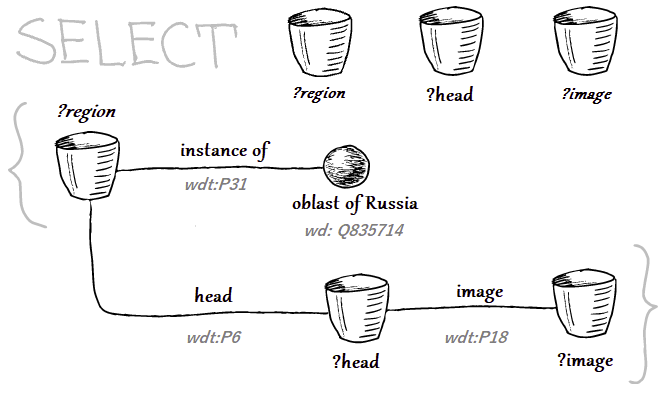
\includegraphics[width=0.99\linewidth]{./intro/bucketsAndBalls/Query_in_basket_and_balls_notation_with_ids.png}
\caption{Запрос в нотации <<Корзины и мячи>> с номерами свойств и объектов Викиданных}
\label{fig:Query_in_basket_and_balls_notation_with_ids}
\end{marginfigure}

Метка (\textit{Label})~--- это то, что есть у каждого мяча, то есть объекта Викиданных. 
Метка~--- это имя, позволяющее различать объекты между собой. 
В Викиданных есть сервис, упрощающий вывод меток, 
для этого достаточно добавить в запросе в конец имени переменной слово \textit{Label}.
Чтобы активировать этот сервис, на новой строке внутри фигурных скобок наберите Ctrl~+~пробел; 
когда вы начнёте писать слово \textit{Label}, тогда будет добавлена строка с этим сервисом\footnote[][12pt]{%
%
Пример вызова этого сервиса представлен в запросе~\ref{lst:regionsOfHeads}, в~строке~8. 
В~этой строке языком для меток указан русский язык (код ru).}. По умолчанию 
вы получаете подсказку с языком интерфейса 
и английским языком в качестве альтернативы, если метка недоступна на языке выбранного интерфейса Викиданных.


Викиданные полны таких замечательных сервисов, и для окончательного запроса мы воспользуемся ещё одним. 
Чтобы получить результат сразу в виде набора фотографий глав областей, 
без дополнительного нажатия на значок глаза, поместите где-нибудь в своём запросе следующую конструкцию для WDQS:
\begin{lstlisting}[ language=SPARQL ]
#defaultView:ImageGrid
\end{lstlisting}

На самом деле не всё нужно писать вручную. Когда вы начнёте набирать текст, сервис автозаполнения предложит варианты.


\newpage
Итоговый запрос~\ref{lst:regionsOfHeads} позволил нам получить требуемую сетку фотографий 
с подписью в виде названия файла иллюстрации, имени руководителя и названия области (рис.~\ref{fig:Result_of_the_request}).

\lstset{numbers=left, firstnumber=1, frame=single}
\begin{lstlisting}[ language=SPARQL, 
                    caption={\href{https://w.wiki/4ENR}{Список руководителей областей России с фотографиями}\protect\footnotemark}, 
                    label=lst:regionsOfHeads, ]
# List of regions of the Russia and images of heads of government
#defaultView:ImageGrid
SELECT DISTINCT ?region ?regionLabel ?head ?headLabel ?image
{
  ?region wdt:P31 wd:Q835714; # ?region is Oblast of Russia
          wdt:P6  ?head.      #         has head of government
  ?head  wdt:P18 ?image.      # head has image
  SERVICE wikibase:label {bd:serviceParam wikibase:language "ru"} 
}
\end{lstlisting}
\footnotetext{Получено: 44 области России и список их руководителей. Ссылка на SPARQL-запрос: \href{https://w.wiki/4ENR}{https://w.wiki/4ENR}.}

%\begin{fullwidth}
\begin{figure*}[h!]
\includegraphics[width=0.9\linewidth]{./intro/bucketsAndBalls/result_of_request_for_photos_of_heads_of_government.png}
    \caption[Сетка фотографий руководителей областей.]{Руководители областей: их имена и фотографии, названия областей. Результат запроса~\protect\ref{lst:regionsOfHeads} в виде сетки изображений}
    \label{fig:Result_of_the_request}
\end{figure*}
%\end{fullwidth}

Такое представление о запросах SPARQL, как о связанных корзинах и мячах, может быть полезным, 
по крайней мере, в начале освоения Викиданных. 
И, конечно, у каждой метафоры есть свои ограничения. 
Например, нельзя поместить один и тот же мяч в две разные настоящие корзины, 
но в~эти виртуальные~--- можно. 
<<Корзины и мячи>> могут быть полезны, чтобы вскарабкаться на~высоту абстракции Викиданных.




\pagelayout{wide} % No margins
\addpart{Examples with Wikidata objects}
\pagelayout{margin} % Restore margins

\chapter{Воздушные суда и их производители}%
\label{ch:aircraft-chapter}

Эта глава посвящена исследованию различных свойств воздушных судов на основе базы Викиданные. 
В ходе исследования с помощью SPARQL-запросов, вычисляемых на объектах типа <<Воздушные суда>>, 
получен список воздушных судов и их производителей, 
а также число выпущенных самолётов для разных моделей. Для этого числа самолётов по моделям проверено выполнение \href{https://w.wiki/vDs}{закона Парето}. 
Также получена диаграмма, отражающая соотношение общего количества производителей воздушных судов по странам. 
В заключение получена оценка полноты данных, представленных в Википедии и Викиданных. 
Согласно ей, в Викиданных представлено всего 595 записей о~производителях воздушных судов из \num{1700} на 2020 год.
Если считать, что ежегодно будет появляться фиксированное количество новых авиапроизводителей 
и количество ежегодно заносимых записей в Викиданные останется неизменным, 
то можно предположить, что примерно через 75~лет (то есть в 2095 году) Викиданные будут содержать записи обо всех авиапроизводителях.

\section{Список самолётов}

Воздушное судно~--- летательный аппарат, поддерживаемый в атмосфере 
за счёт взаимодействия с воздухом, отличного от взаимодействия с воздухом, отражённым от поверхности земли или воды.
К воздушным судам относятся следующие виды летательной техники: 
автожир, аэростат, вертолёт, винтокрыл, дирижабль, махолёт, планёр и самолёт.
К воздушным судам не относятся космические корабли, ракеты, экранопланы (но~не~экранолёты) и суда на~воздушной подушке. 

Построим список воздушных судов с помощью запроса~\ref{lst:aircraftList}. 
Здесь мы работаем с объектом <<Воздушные суда>> \href{https://www.wikidata.org/wiki/Q11436}{Q11436}.

\newpage 

%\begin{itemize}
%\itemОбъект: Воздушное судно (Q11436).
%\itemСвойство: Экземпляр (P31).
%\end{itemize}

\begin{lstlisting}[ 
            language=SPARQL, 
            caption={\href{https://w.wiki/t3j}{Список воздушных судов}\protect\footnotemark}, 
            label=lst:aircraftList, 
            numbers=none,
         ]
#List of `instances of` "aircraft"
SELECT ?plane ?planeLabel
WHERE
{
    ?plane wdt:P31 wd:Q11436. # instances of aircraft
    SERVICE wikibase:label { bd:serviceParam wikibase:language "ru" }
}
\end{lstlisting}
\footnotetext{Получено: 153 воздушных судна в 2017 году, 299 воздушных судов в 2020 году. Ссылка на SPARQL-запрос: \href{https://w.wiki/t3j}{https://w.wiki/t3j}.}

%Результатом запроса~\ref{lst:aircraftList} (на английском языке) является список всех воздушных судов. На 2017 год список содержал \num{1564} записи, а к 2020 году число записей увеличилось до \num{3325}.
%На руском языке на 2017 год результат запроса~\ref{lst:aircraftList} содержал 153 записи, а к 2020 году их число увиличилось до 299 записей.

Наиболее полными и проработанными воздушными судами на Викиданных по числу свойств 
на~2017 год являются: \href{https://www.wikidata.org/wiki/Q271446}{МиГ-3}, 
\href{https://www.wikidata.org/wiki/Q1349098}{Як-36}, 
\href{https://www.wikidata.org/wiki/Q429839}{Mitsubishi A5M}. 
На 2020 год~--- \href{https://www.wikidata.org/wiki/Q770863}{Sopwith Triplane} (18 свойств), 
\href{https://www.wikidata.org/wiki/Q1658673}{Ил-103} (14 свойств) и 
\href{https://www.wikidata.org/wiki/Q665071}{Martin 2-0-2} (14 свойств).
Количество свойств было получено с помощью сервиса~\href{https://prowd.id/dashboards/972cd00ce110/profile}{ProWD}\autocite{aircraft_prowd}, 
анализирующем заданный объект Викиданных.
%Почти пустыми и малоинформативными воздушными судами на 2017 год оказались: \href{https://www.wikidata.org/wiki/Q464247}{МиГ-1}, \href{https://www.wikidata.org/wiki/Q2296502}{Су-6}, \href{https://www.wikidata.org/wiki/Q1658673}{Ил-103}.
На 2020 год малоинформативными воздушными судами оказались: 
\href{https://www.wikidata.org/wiki/Q820603}{Бе-1} (3 свойства), 
\href{https://www.wikidata.org/wiki/Q117984}{Литуаника} (4 свойства) и 
\href{https://www.wikidata.org/wiki/Q572762}{Ла-168} (3 свойства).



\section{Производители воздушных судов}%
\marginnote{\MarginQuestion У каких из представленных ниже российских производителей самолётов есть веб-сайты?%}
\begin{itemize}
%\item \href{https://w.wiki/vDw}{Миг}
\item \ruwiki{vDw}{МиГ}
\item \ruwiki{vDx}{Саратовский авиационный завод}
\item \ruwiki{vDy}{Туполев}
\item \ruwiki{vDz}{Сухой}
\end{itemize}
См. ответ~\ref{answer:aircraft_manufacturers} на с.~\pageref{answer:aircraft_manufacturers}.
}

Построим список производителей воздушных судов, выполнив запрос~\ref{lst:lang2}.

\index{SPARQL!COUNT!Производители воздушных судов}
\begin{lstlisting}[ 
            language=SPARQL, 
            caption={\href{https://w.wiki/t3n}{Производители воздушных судов}\protect\footnotemark}, 
            label=lst:lang2, 
            numbers=none,
            ]
# Count aircraft having property manufacture, group by manufacture
SELECT ?manufacture ?manufactureLabel (COUNT(?plane) AS ?count) 
WHERE {
  ?plane wdt:P31 wd:Q11436.     # instance of aircraft
  ?plane wdt:P176 ?manufacture. # manufacture
  SERVICE wikibase:label { bd:serviceParam wikibase:language "ru" }
}
GROUP BY ?manufacture ?manufactureLabel
\end{lstlisting}
\footnotetext{Получено: 300 производителей воздушных судов в 2017 году, 590 производителей воздушных судов в 2020 году. Ссылка на SPARQL-запрос: \href{https://w.wiki/t3n}{https://w.wiki/t3n}.}

Результатом запроса~\ref{lst:lang2} является список всех производителей воздушных судов с указанием количества различных моделей, производимых данным заводом.



\section{Количество выпущенных воздушных судов}%
\marginnote{%
\label{aircraft_question_2} 
\MarginQuestion Найдите соответствие между датой основания и компанией в следующей таблице:
\\
\begin{tabular}{ l | l }
Компания & Дата основания \\ \hline
\ruwiki{vDw}{Миг} & 1939 \\
\ruwiki{vE4}{Вымпел} & 18 ноября 1949 \\
\ruwiki{vDy}{Туполев} & 8 декабря 1939 \\
\ruwiki{vDz}{Сухой} & 22 октября 1922 \\
\end{tabular}
\\
См. ответ~\ref{answer:aircraft_company_foundation_date} на с.~\pageref{answer:aircraft_company_foundation_date}.
}

Авиационная промышленность~--- это одна из самых крупных отраслей машиностроения в мире. 
В её задачи входит как разработка, так и производство различной воздушной техники. 
Для~того чтобы оценить, какие модели воздушных судов являются самыми массовыми, 
мы построим диаграмму произведённых судов различных моделей 
с помощью запроса~\ref{lst:lang3}.

\begin{lstlisting}[ 
            language=SPARQL, 
            caption={\href{https://w.wiki/v4J}{Список моделей, упорядоченный по количеству выпущенных самолётов}\protect\footnotemark}, 
            label=lst:lang3, 
            numbers=none,
            ]
# List of aircraft models, sorted by number of aircraft built
SELECT ?plane ?planeLabel ?planes_produced WHERE {
  ?plane wdt:P31 wd:Q11436. # instance of aircraft
  ?plane wdt:P1092 ?planes_produced.  # total aircraft manufactured
  SERVICE wikibase:label {bd:serviceParam wikibase:language "ru,en"}
}
ORDER BY DESC(?planes_produced)
\end{lstlisting}
\footnotetext{Получено: 288 моделей, для которых известно число выпущенных самолётов, 2020 год. Ссылка на SPARQL-запрос: \href{https://w.wiki/v4J}{https://w.wiki/v4J}.}

%В результатом запроса~\ref{lst:lang3} мы получили список состоящий из 177 записей (на 2020 год) моделей воздушных судов и их суммарного произведенного количества за всё время.


На~рис.~\ref{fig:Number_of_aircraft_produced_ru_2020} видно, 
что на 2020 год больше всего было выпущено воздушных судов следующих моделей: 
\href{https://www.wikidata.org/wiki/Q2096452}{Piper PA-32} (\num{7842} штук), 
\href{https://www.wikidata.org/wiki/Q1860367}{Piper PA-24 Comanche} (\num{4857}), 
\href{https://www.wikidata.org/wiki/Q694521}{Junkers W 34} (\num{3000}), 
\href{https://www.wikidata.org/wiki/Q4046989}{Piper J-4}~(\num{1251}).

%По диаграмме видно, что больше всего было выпущено воздушных судов следующих моделей: Piper PA-32 (\num{7842} штук), Piper PA-24 Comanche (\num{4857}), Junkers W 34 (\num{3000}), Piper J-4 (\num{1251})

\begin{marginfigure}
    \setlength{\fboxsep}{0pt}%
    \setlength{\fboxrule}{1pt}%
    \fcolorbox{gray}{gray}{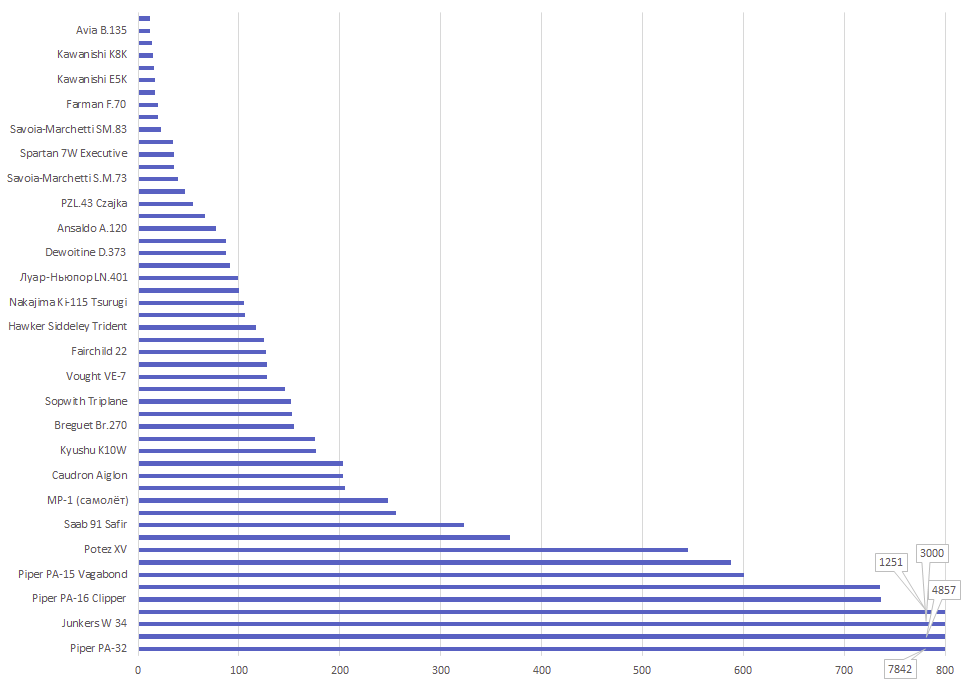
\includegraphics[width=0.99\linewidth]{./chapter/aircraft/Number_of_aircraft_produced_ru_2020.png}}%
%	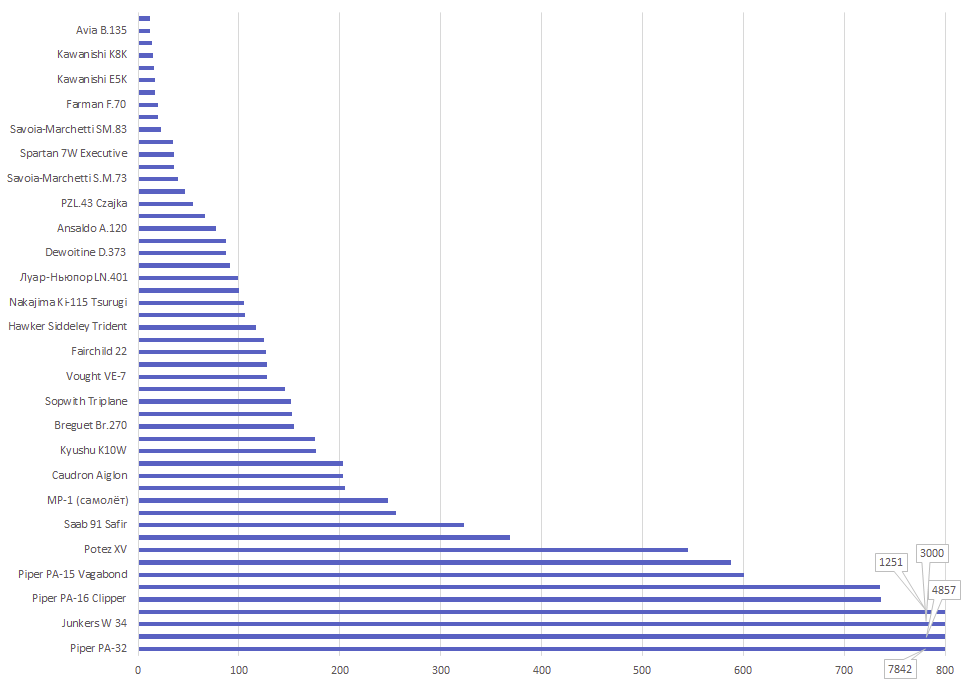
\includegraphics{./chapter/aircraft/Number_of_aircraft_produced_ru_2020.png}%
	\caption[Количество выпущенных воздушных судов по моделям, 2020 год.]{Количество выпущенных воздушных судов по моделям, 2020. Диаграмма построена в Microsoft Excel на основе данных, полученных с помощью запроса~\protect\ref{lst:lang3_1}}%
    \label{fig:Number_of_aircraft_produced_ru_2020}%
\end{marginfigure}

Некоторые модели воздушных судов были выпущены в единичных экземплярах, 
поэтому для~повышения читабельности диаграммы 
(рис.~\ref{fig:Number_of_aircraft_produced_ru_2020}) их можно исключить. 
Для получения нового списка добавим в запрос~\ref{lst:lang3_1} фильтр по количеству выпущенных самолётов.


\index{SPARQL!FILTER!Список выпущенных самолётов, в количестве более 10 штук}
\begin{lstlisting}[ 
            language=SPARQL, 
            caption={\href{https://w.wiki/v4N}{Список, включающий только те самолёты, которые были выпущены в количестве более 10 штук}\protect\footnotemark}, 
            label=lst:lang3_1, 
            numbers=none,
            ]
# List of aircraft models, sorted by number of aircraft built
#defaultView:BarChart
SELECT ?plane ?planeLabel ?planes_produced WHERE {
  ?plane wdt:P31 wd:Q11436. # instance of aircraft
  ?plane wdt:P1092 ?planes_produced.  # total aircraft manufactured
  FILTER (?planes_produced > 10)
  SERVICE wikibase:label {bd:serviceParam wikibase:language "ru,en"}
}
ORDER BY (?planes_produced)
\end{lstlisting}
\footnotetext{Получен отфильтрованный по количеству выпущенных самолётов список, 
состоящий из 124 моделей. Ссылка на SPARQL-запрос: \href{https://w.wiki/v4N}{https://w.wiki/v4N}.}

%Итого, результатом запроса~\ref{lst:lang3_1} уже будет 86 записей, а не 177.



\newpage 
Теперь 
\marginnote[0cm]{%
\label{aircraft_question_3}%
\MarginQuestion Найдите соответствие между расположением штаб-квартиры компании и названием компании производителя самолётов в следующей таблице:
\\
\begin{tabular}{ l | l }
Компания & Штаб-квартира \\ \hline
\ruwiki{vEP}{Камов} & Улан-Удэ \\
\ruwiki{vER}{Авиадвигатель} & Пермь \\
\ruwiki{vEL}{Улан-Удэнский завод} & Москва \\
\ruwiki{vDz}{Сухой} & Люберцы \\
\end{tabular}
\\
См. ответ~\ref{answer:aircraft_company_headquarters} на с.~\pageref{answer:aircraft_company_headquarters}.
}
 попытаемся ответить на вопрос: выполняется ли \ruwiki{vDs}{Закон Парето} относительно числа моделей самолётов?
Чтобы построить график процентного соотношения количества выпущенных моделей самолётов 
к общему числу произведённых самолётов, необходимо выполнить следующие шаги:

%\footnotetext{Диаграмма~\ref{fig:Number_of_aircraft_produced_ru_2020} была построена в excel на основании данных, полученных из запроса~\ref{lst:lang3_1}}.

\begin{enumerate} 
  \item Подсчитать общее число самолётов по всем моделям с помощью запроса~\ref{lst:lang3_2}.
  
  \index{SPARQL!SUM!Общее число произведённых самолётов}
\begin{lstlisting}[ language=SPARQL, 
        caption={\ruwiki{vE9}{Общее число произведённых самолётов}\protect\footnotemark}, 
        label=lst:lang3_2, 
        numbers=none, 
        ]
SELECT (SUM(?count) as ?sum) WHERE {
  SELECT ?count WHERE {
    ?plane wdt:P31 wd:Q11436; # instance of aircraft
		   wdt:P1092 ?count. # total aircraft production
  }
}
\end{lstlisting}
\footnotetext{Общее число выпущенных самолётов на 2020 год составляет \num{44151}. 
        Ссылка на SPARQL-запрос: \ruwiki{vE9}{https://w.wiki/vE9}.}
  
  %В результате выполнения запроса~\ref{lst:lang3_2} мы получили общее число выпущенных самолётов на 2020 год = \num{33177}.
  
  \item По оси $X$ отложить число рассматриваемых моделей самолётов 
      (то есть при $x = 1$ мы рассматриваем число выпущенных самолётов первой модели, 
        при $x = 2$~--- число выпущенных самолётов первой и второй модели и так далее). 
        По оси $Y$ взять значение $F(n) = \sum\limits_{i=1}^n f(i)$, 
        где $f(i)$~--- число выпущенных самолётов модели $i$. 
        При этом выполняется условие $f(i) > f(j)$, при $i < j$, 
        где $i$, $j$~--- номер модели самолёта 
        (то есть модели самолётов заранее упорядочены так, что 
        первых моделей произведено больше, чем последующих, это хорошо видно на рис.~\ref{fig:Pareto_principle_diargam}). 
        Также по оси $X$ следует отложить вторую шкалу от 0 до 1, 
        чтобы легче было определить параметры для проверки выполнения \ruwiki{vDs}{закона Парето}.
\end{enumerate}

По графику, представленному на рис.~\ref{fig:Pareto_principle_diargam}, видно, 
что 80\,\% всех выпущенных самолётов приходится на 16 различных моделей самолётов, 
что составляет 9,2\,\% от общего числа моделей. 
Закон Парето утверждает, что 
\ruwiki{vDs}{«20\,\% усилий дают 80\,\% результата, 
а остальные 80\,\% усилий~--- лишь 20\,\% результата»}. 
Можно сделать вывод, что выполняется более сильный закон, чем принцип Парето, относительно числа моделей самолётов.
\footnotetext{Закон Парето: \href{https://w.wiki/vDs}{https://w.wiki/vDs}.}

\newpage 
\begin{figure*}[h!]

    \setlength{\fboxsep}{0pt}%
    \setlength{\fboxrule}{1pt}%
    \fcolorbox{gray}{gray}{\includegraphics[width=0.99\linewidth]{./chapter/aircraft/Pareto_principle_diargam.png}}%
%	\includegraphics{./chapter/aircraft/Number_of_aircraft_produced_ru.png}%
	\caption{Процентное соотношение количества выпущенных моделей самолётов по $n$ моделям к общему числу выпущенных самолётов за всё время, 2020 год}%
    \label{fig:Pareto_principle_diargam}%
\end{figure*}






\newpage 
\label{aircraft_question_4}
\marginnote[8pt]{
    \MarginQuestion
    Как называется воздушное судно, удерживаемое в воздухе огромным баллоном с горючим смертельно опасным газом, расположенным прямо над головами пассажиров?
\\
См. ответ~\ref{answer:aircraft_question_airship} на с.~\pageref{answer:aircraft_question_airship}.
}
\section{В каких странах производят самолёты}

Построим список количества производителей воздушных судов по странам. 
Для~выполнения запроса~\ref{lst:lang5} 
используем группировку по странам (\lstinline|GROUP BY|) 
и при помощи функции \lstinline|Count()| 
для~каждой страны подсчитаем общее количество авиастроительных заводов.

%\index{SPARQL!COUNT!Список соотношения количества производителей воздушных судов по странам}
%\begin{lstlisting}[ language=SPARQL, caption={\href{https://w.wiki/t3t}{Список стран с указанием количества производителей воздушных судов}\protect\footnotemark}, label=lst:lang4, ]
%# Count manufacture having property country group by country
%SELECT ?country ?countryLabel (count(?manufacturer) as ?count)
%WHERE
%{
%    ?manufacturer wdt:P31 wd:Q936518.   # instance of aerospace manufacture
%    ?manufacturer wdt:P17 ?country.     # belong to country
%    SERVICE wikibase:label {bd:serviceParam wikibase:language "ru"}
%}
%GROUP BY ?country ?countryLabel
%\end{lstlisting}
%\footnotetext{Получено 39 стран, выпускающих самолёты в 2017 году, 46 стран, выпускающих самолёты в 2020 году. Ссылка на SPARQL-запрос: \href{https://w.wiki/t3t}{https://w.wiki/t3t}}

%В результатом запроса~\ref{lst:lang4} мы получили список состоящий из 39 записей (на 2017 год): страна и количество производств воздушных судов. К 2020 году число записей в русском сегменте Викиданных возросло до 46 записей.

Получив список стран по количеству заводов-производителей авиационной техники, 
построим пузырьковую диаграмму 
соотношения количества производителей воздушных судов по странам 
с~помощью запроса~\ref{lst:lang5}.

\begin{marginfigure}[0\baselineskip]
\centering
	\includegraphics[width=0.82\textwidth]{./chapter/aircraft/Manufacture-with-country_2017.png}
	\caption{Соотношение количества производителей воздушных судов по странам, 2017 год}
	\label{fig:Manufacture_with_country_2017}
\end{marginfigure}


\index{SPARQL!COUNT!Соотношение количества производителей воздушных судов по странам}
\index{График!BubbleChart!Соотношение количества производителей воздушных судов по странам}
\begin{lstlisting}[ language=SPARQL, 
                caption={\href{https://w.wiki/t3v}{Список стран с указанием количества производителей воздушных судов}\protect\footnotemark}, 
                label=lst:lang5, ]
#defaultView:BubbleChart
SELECT ?country ?countryLabel (count(?manufacturer) as ?count)
WHERE
{
    ?manufacturer wdt:P31 wd:Q936518. # instance of aerospace manufacture
  	?manufacturer wdt:P17 ?country. # belong to country
    SERVICE wikibase:label {bd:serviceParam wikibase:language "ru"}
}
GROUP BY ?country ?countryLabel
\end{lstlisting}
\footnotetext{Получено: 39 стран, выпускающих самолёты в 2017 году, 46 стран, выпускающих самолёты в 2020 году. Ссылка на SPARQL-запрос: \href{https://w.wiki/t3v}{https://w.wiki/t3v}.}

\begin{marginfigure}
\centering
	\includegraphics[width=0.62\textwidth]{./chapter/aircraft/Manufacture-with-country_2020.png}
	\caption{Соотношение количества производителей воздушных судов по странам, 2020 год}
	\label{fig:Manufacture_with_country_2020}
\end{marginfigure}

В результате выполнения запроса~\ref{lst:lang5} будут построены пузырьковые диаграммы 
(рис.~\ref{fig:Manufacture_with_country_2017} и~\ref{fig:Manufacture_with_country_2020}), 
в которых круги означают страны, 
а их размеры соответствуют количеству авиапроизводителей в указанной стране. 
Такие диаграммы помогают более наглядно увидеть разницу в количестве авиационных заводов в разных странах.


%Больше всего производителей указано у США (115), Великобритании (30), Германии (17), России (17) на 2017 год.

%\begin{figure}[h!]
%\centering
%	\includegraphics[width=0.75\textwidth]{./chapter/aircraft/Manufacture-with-country_2020.png}
%	\caption{Соотношение количества производителей воздушных судов по странам, 2020 год.}
%	\label{fig:Manufacture_with_country_2020}
%\end{figure}

Сравнивая две пузырьковые диаграммы за 2017 (рис.~\ref{fig:Manufacture_with_country_2017}) и 2020 (рис.~\ref{fig:Manufacture_with_country_2020}) годы, можно сделать вывод, что основными производителями воздушных судов в мире 
в 2017 и 2020 годах были: США (115 заводов в 2017-м и 135 заводов в 2020 году), Великобритания (30 и 43 завода), Германия (17 и 26 заводов) и Россия (17 и 21 завод). Лидером по-прежнему является США, 
а вот Франция за 3 года сумела опередить Германию, 
увеличив количество производств до 29 (Германия~--- 26), 
тем самым заняв третье место. 
%Но в целом соотношение по производству воздушных судов между различными странами остаётся на прежнем уровне.
В целом соотношение по странам остаётся прежнем.

Ответ на запрос~\ref{lst:lang2} показывает, 
что Викиданные содержат неполный список производителей воздушных судов 
по сравнению с данными сайта \href{https://www.aviationfanatic.com/}{aviationfanatic.com}. 
Исследуем вопрос полноты Викиданных ниже. 

%\begin{figure}[!h]
%   \begin{floatrow}
%\ffigbox{\includegraphics[width=\linewidth]{./chapter/aircraft/Manufacture-with-country_2017.png}}%
%        {\caption{Соотношение количества производителей воздушных судов по странам, 2017 год.}\label{fig:Manufacture_with_country_2017}}
%\hfill
%\ffigbox{\includegraphics[width=\linewidth]{./chapter/aircraft/Manufacture-with-country_2020.png}}%
%        {\caption{Соотношение количества производителей воздушных судов по странам, 2020 год.}\label{fig:Manufacture_with_country_2020}}
%  \end{floatrow}
%\end{figure}

%\begin{fullwidth}
%\noindent\begin{minipage}[]{.46\linewidth}
%    \centering
%	    \includegraphics[width=0.99\linewidth]{./chapter/aircraft/Manufacture-with-country_2017.png}
%     \captionof{figure}{Соотношение количества производителей воздушных судов по странам, 2017 год.}
%   	    \caption{Соотношение количества производителей воздушных судов по странам, 2017 год.}
%	    \label{fig:Manufacture_with_country_2017}
%\end{minipage}%
%just a break for lines between two columns of listings
%\hfill
%\begin{minipage}[]{.46\linewidth}
%    \centering
%	\includegraphics[width=0.9\linewidth]{./chapter/aircraft/Manufacture-with-country_2020.png}
%   	\caption{Соотношение количества производителей воздушных судов по странам, 2020 год.}
%	\label{fig:Manufacture_with_country_2020}
%\end{minipage}
%\end{fullwidth}%




%\begin{fullwidth}
%\begin{figure*}[h!]
%%\begin{marginfigure}
%%\centering
%%	\includegraphics[width=0.55\textwidth]{./chapter/aircraft/Manufacture-with-country_2017.png}
%%	\caption{Соотношение количества производителей воздушных судов по странам, 2017 год}
%%	\label{fig:Manufacture_with_country_2017}
%\end{figure*}
%%\end{marginfigure}
%%\begin{marginfigure}
%\begin{figure*}[h!]
%%\centering
%%	\includegraphics[width=0.55\textwidth]{./chapter/aircraft/Manufacture-with-country_2020.png}
%%	\caption{Соотношение количества производителей воздушных судов по странам, 2020 год}
%%	\label{fig:Manufacture_with_country_2020}
%\end{figure*}
%%\end{marginfigure}
%\end{fullwidth}%





\section{Полнота Викиданных по числу производителей воздушных судов}

Согласно сайту \href{https://www.aviationfanatic.com/}{aviationfanatic.com}, 
существовало около \num{1700} производителей воздушных судов 
на 2017 год и 1939 судов на 2020 год\autocite{count_of_aircraft_manufactures}, 
но SPARQL-запрос~\ref{lst:lang2} вернул всего 300 авиазаводов в~Викиданных в 2017 году 
и 595 авиазаводов в 2020 году. Из этого можно сделать вывод о~неполноте Викиданных.  

Попробуем спрогнозировать, когда Викиданные будут описывать не меньше самолётов, 
чем сайт aviationfanatic.com. 
За три года количество производителей воздушных судов увеличилось на 239, 
что составляет ежегодный прирост примерно на 80 авиапроизводителей. 
Также за это время в Викиданные была занесена информация о 295 авиапроизводителях, 
то есть ежегодно добавляется около сотни авиазаводов. 
На 2020 год в Викиданных не было информации о \num{1344} авиапроизводителях, 
представленных на сайте \href{https://www.aviationfanatic.com/}{aviationfanatic.com}. 
Если считать, что ежегодно будет добавляться фиксированное количество новых авиапроизводителей 
и количество ежегодно заносимых записей в Викиданные останется неизменным, 
то можно предположить, что примерно через 75 лет (то есть в 2095 году) 
Викиданные будут содержать записи обо всех авиапроизводителях, представленных на сайте aviationfanatic.com.

В категории Википедии \ruwiki{vF4}{<<Авиастроительные компании России>>}\sidenote{%
%
См. \href{https://w.wiki/vF4}{https://w.wiki/vF4}.%
%
} указано наличие в России 58 авиастроительных компаний в 2017 году 
и 62 заводов, институтов и корпораций, связанных с~самолётостроением, в 2020 году, 
но в то же время на сайте \href{https://www.aviationfanatic.com/}{aviationfanatic.com} 
указано наличие 61 завода\autocite{count_plants_of_aircrafts} в 2017 году 
и 71 предприятия в 2020 году. 
Среди авиастроительных компаний России 
представлены такие компании как: \ruwiki{vNY}{Иркут}, \ruwiki{vDw}{МиГ}, \ruwiki{vDy}{Туполев}.

%\section{Степень заполненности Викиданных}

%Для заполнения были выбраны поля label и description у объектов, перечисленных в категории <<Авиастроительные компании России>>. Так как объектов там много, было решено автоматизировать заполнение, для чего была написана соответствующая программа. Для начала был создан JSON-файл с объектами из категории и пустыми полями для заполнения:

%\begin{lstlisting}[ language=SPARQL, label=lst:lang6, ]
%{
%  "121 авиационный ремонтный завод": {
%    "description": "",
%    "descriptionen": "",
%    "nameen": "",
%    "qid": "Q4028573"
%    },
%  ...
%}
%\end{lstlisting}

%В первой части программы записывались уже существующие значения полей из Викиданных в JSON-файл. После чего было необходимо заполнить оставшиеся пустыми поля, то есть поля, не заполненые в Викиданных. В итоге JSON-файл выглядел примерно так:

%\begin{lstlisting}[ language=SPARQL, label=lst:lang7, ]
%{
%  "121 авиационный ремонтный завод": {
%    "description": "авиаремонтное предприятие, расположенное посёлке Старый Городок",
%    "descriptionen": "aircraft repair facility, located in the village Stary Gorodok",
%    "nameen": "121 aircraft repair plant",
%    "qid": "Q4028573"
%  },
%  ...
%}
%\end{lstlisting}

%Во второй части программы записывались данные из JSON-файла в Викиданные.

%С помощью этой программы удалось упростить работу с Викиданными, так как не приходилось самостоятельно заходить на страницы объектов и вносить изменения, если существующие данные не удовлетворяют ожиданиям, то есть поле в Викиданных отличается от локального.

\section{Упражнения}%
%\noindent\begin{marginfigure}[4\baselineskip]%
\marginnote{%
\MarginQuestion Какое воздушное судно здесь изображено?\\
{%
\setlength{\fboxsep}{0pt}%
\setlength{\fboxrule}{1pt}%
\fcolorbox{gray}{gray}{\includegraphics[width=0.7\linewidth]{./chapter/aircraft/airship-SSSR-V6.jpg}}%
}%
%    \caption[Неизвестное воздушное судно.]{

См. ответ~\ref{answer:aircraft_question_airship_2} на с.~\pageref{answer:aircraft_question_airship_2}.
%} eo caption
\label{fig:airship_question_aircraft}%
} % eo sidenote
%\end{marginfigure}%


\begin{enumerate}
\item Найти самолет с максимальным радиусом полета.
\item Отметить на политической карте мира местоположение главных офисов компаний авиапроизводителей.
\item Найти производителя с максимальным числом изготовленных самолетов, используя свойство \href{https://w.wiki/vF7}{\textit{manufacturer (P176)}} у воздушных судов.
\item Когда был построен первый самолёт?
\item Какие фирмы первыми выпустили 10, 100 и 1000 самолётов?
\item Нарисуйте диаграмму количества выпускаемых самолётов в мире и в России по годам.
\end{enumerate}

\hyphenation{аудио-драмах}
\hyphenation{аудио-записях}

% Newline in table of contents, see https://tex.stackexchange.com/q/170724/99685
\addtocontents{toc}{\protect\pagebreak[4]}
\chapter{Аниме: загадочный и поразительный мир японской анимации}
\label{ch:anime}

В рамках этой главы исследуется объект Викиданных \wdqName{<<аниме>>}{1107}. 
С помощью SPARQL-запросов, вычисляемых на объектах типа <<аниме>> в Викиданных, 
получен список сэйю\sidenote[][-1\baselineskip]{%
%
Сэйю~--- это японские актёры озвучивания. 
Сэйю обычно озвучивают роли персонажей в аниме, видеоиграх, фильмах, 
а также на радио и телевидении или выступают в роли рассказчика в радиопостановках. 
Кроме того, голоса сэйю используются в~рекламе, голосовых объявлениях, 
аудиозаписях книг и учебных материалов, а~также для переозвучивания. 
Сэйю могут быть как мужчины, так~и~женщины, как~взрослые, так и дети.% eo sidenote

\vspace{5pt}
\includegraphics[width=0.5\linewidth]{chapter/anime/seyu.jpg}

\noindent Сэйю Кэндзи Акабанэ озвучивал роль персонажа Sasuke Sarutobi в видеоигре Ikemen Sengoku, 2018 год. 
Wikimedia Commons / numan (CC BY-SA)
\vspace{5pt}
%
}, упорядоченный по числу озвученных ими аниме, 
построен график числа аниме, озвученных одним сэйю, 
построен граф, связывающий сэйю
и озвученные ими аниме, получена оценка трудоспособного возраста сэйю. 

%%%\begin{marginfigure}[0.0cm]{
%	\setlength{\fboxsep}{0pt}%
%	\setlength{\fboxrule}{1pt}%
%	\fcolorbox{gray}{gray}{
%%%    \includegraphics[width=0.5\linewidth]{chapter/anime/seyu.jpg}%}
%%}
%%%\caption[Сэйю Кэндзи Акабанэ.]%
%%%        {Сэйю Кэндзи Акабанэ озвучивал роль персонажа Sasuke Sarutobi в видеоигре Ikemen Sengoku, 2018 год. 
%%%Wikimedia Commons / numan (CC BY-SA)}
%%%\label{fig:seiyu}
%%\end{marginfigure}

\section{Экземпляры объекта <<Аниме>>}

Аниме~--- это японская мультипликация. 
Она стоит особняком и выделяется своим визуальным стилем, 
однако есть и менее очевидные отличия: 
так, по сравнению с американской и японской анимацией у аниме значительно шире список жанров~--- 
от детских и семейных комедий до драматических историй, 
которые на Западе обычно представляются только в фильмах 
с~живыми актёрами\sidenote{%   \autocite{sister_city}
%
    Slowpoke T. Аниме vs мультипликация. 2020. 
    URL: \href{https://cadelta.ru/anime/id6119}
              {https://cadelta.ru/anime/id6119}.%
}. % eo sidenote


У каждого аниме есть свои актёры озвучивания. 
В дальнейшем под <<сэйю>> будем понимать японского актёра озвучивания. 
В японской анимации слова <<актёры озвучивания>> и <<сэйю>> являются синонимами\sidenote{%
%
    Шикимори~--- энциклопедия аниме и манги. 
    URL:~\href{https://shikimori.one/}
              {https://shikimori.one/}.%
}.\, % eo sidenote
%
Под словом <<тайтл>> (от англ. \emph{title}, \emph{название}) обычно понимают конкретное аниме\autocite{anime_social}. 
В~общем же смысле слово <<тайтл>> означает понятие, объединяющее различные виды продукции 
(от~кино\-фильма до~романа), созданные на основе конкретного произведения, за которым закреплено строго определённое название\autocite{anime_title_def}.

Чтобы работать со списком аниме в Викиданных, 
нам понадобятся объект \wdqName{<<аниме>>}{1107} и свойство \wdProperty{31}{<<экземпляр>>}. 
Получим список всех аниме без учёта подклассов (запрос~\ref{lst:anime}).

\newpage

\begin{lstlisting}[ language=SPARQL, 
                    caption={\href{https://w.wiki/4ABw}{Список аниме без учёта подклассов}\protect\footnotemark},
                    label=lst:anime,
                    texcl,
                    numbers=none,
                    ]
# List of instances of anime
SELECT ?anime ?animeLabel
WHERE
{
    ?anime wdt:P31 wd:Q1107. # instance of anime
    SERVICE wikibase:label{bd:serviceParam wikibase:language "ru,en,ja"}
}
\end{lstlisting}%
\footnotetext{Получено: \num{683} результата в 2017 году и \num{216} результатов в 2021 году. Ссылка на~SPARQL-запрос: \href{https://w.wiki/4ABw}{https://w.wiki/4ABw}.}

\index{График!Sunburst diagram}
\begin{marginfigure}[1\baselineskip]
{\includegraphics[width=0.5\linewidth]{chapter/anime/anime-subclasses-sunburst-diagram-2021.png}}
\vspace{-7pt}
\caption{Жанры аниме на круговой диаграмме, 2021 год}%
\label{fig:anime_piechart}
\end{marginfigure}

В действительности в Викиданных объектов аниме гораздо больше, 
но они являются экземплярами не объекта <<аниме>>, а его подклассов, 
таких как, например, \wdqName{<<аниме-сериал>>}{63952888}. 
Чтобы получить список жанров аниме и количество аниме, 
относящихся к этим жанрам, выполним запрос~\ref{lst:anime_w_subclass}.

\begin{lstlisting}[ language=SPARQL, 
                    caption={\href{https://w.wiki/4ABj}{Список жанров аниме и количество аниме, относящихся к этим жанрам}\protect\footnotemark},
                    label=lst:anime_w_subclass,
                    numbers=none,
                    texcl 
                    ]
# Select anime and its subclasses with number of titles
# corresponding to these subclasses
SELECT ?subAnime ?subAnimeLabel (COUNT(?subAnimeInst) AS ?count)
WHERE {
  ?subAnime wdt:P279* wd:Q1107.   # select anime subclass list
  ?subAnimeInst wdt:P31 ?subAnime # link titles and subclasses
    SERVICE wikibase:label{bd:serviceParam wikibase:language "ru,en,ja"}
}
GROUP BY ?subAnime ?subAnimeLabel
ORDER BY DESC(?count)
\end{lstlisting}%
\footnotetext{Получено: \num{11} результатов в 2021 году. Ссылка на~SPARQL-запрос: \href{https://w.wiki/4ABj}{https://w.wiki/4ABj}.}


\index{Визуализация данных!Rawgraphs}
Визуализировать распределение аниме по~жанрам можно в~виде 
круговой диаграммы (рис.~\ref{fig:anime_piechart}). 
построенной с~помощью сервиса 
Rawgraphs (\href{https://app.rawgraphs.io}{https://app.rawgraphs.io}). 
По-английски такой вид диаграм, имеющих радиально расходящиеся лучи, 
называется \emph{sunburst diagram}. 
%
Полученная классификация аниме по жанрам не идеальна, 
так как есть большое смещение в сторону аниме-сериалов: 
из \num{4875} тайтлов \num{2984} отнесены к жанру <<аниме-сериал>> (\num{62,7}\,\%); 
вероятно, классификация жанров аниме в Викиданных требует дальнейшего уточнения. 
Также в подклассы попали понятия, относящиеся не к общей классификации, 
а~к~отдельным аниме, например \href{https://w.wiki/4L5p}{<<Евангелион>>}.



\newpage
Получим список всех аниме, включая тайтлы, относящиеся к жанрам аниме (запрос~\ref{lst:all_anime_list}).

%\begin{minipage}{\linewidth}
\begin{lstlisting}[ language=SPARQL, 
                    caption={\href{https://w.wiki/49zY}{Список всех аниме в Викиданных}\protect\footnotemark},
                    label=lst:all_anime_list,
                    numbers=none,
                    texcl 
                    ]
# List of instances of anime and subclasses of anime
SELECT ?anime ?animeLabel
WHERE
{
    ?anime wdt:P31/wdt:P279* wd:Q1107. # instance of anime/subclass
    SERVICE wikibase:label{bd:serviceParam wikibase:language "ru,en,ja"}
}
\end{lstlisting}%
\footnotetext{Получено: 683 результата в 2017 году и 4875 результатов в 2021 году. Ссылка на~SPARQL-запрос: \href{https://w.wiki/49zY}{https://w.wiki/49zY}.}
%\end{minipage}

Аниме, о которых есть наиболее полная информация на Викиданных~--- 
это \wdqName{Гуррен-Лаганн}{4277}, \wdqName{Space Battleship Yamato}{4292}, 
\wdqName{Project A-ko}{4316}. 
Аниме с~малоинформативными записями на~Викиданных оказались 
\wdqName{Doraemon}{711311}, 
\wdqName{The Animal Conference on the Environment}{97195557}, 
\wdqName{Assassins Pride}{96737300}.

Среди всех аниме-тайтлов в Викиданных больше всего свойств, 
по данным сервиса ProWD, %deadlink \autocite{anime_prowd}, 
у~фильма \wdqName{Fullmetal Alchemist: The Sacred Star of Milos}{1004318}\footnote{%
%
    <<Стальной алхимик: Священная звезда Милоса>>~--- полнометражный аниме-фильм, 
    являющийся продолжением аниме-сериала <<Стальной алхимик>>. 
    Его главные герои~--- братья-алхимики, 
    использующие свои магические способности 
    для~борьбы с силами зла и противостояния преступникам.%
} (\num{24} свойства).



\subsection{Список сэйю, упорядоченный по числу озвученных ими аниме}

Разумеется, в большинстве аниме участвует не один, а множество персонажей. 
Соответственно, разных персонажей озвучивают разные сэйю. 
Большинство сэйю озвучили за свою карьеру несколько тайтлов, 
а многие~--- десятки тайтлов. 
Талантливых сэйю приглашают озвучивать сразу нескольких персонажей в одном аниме. Одним из самых популярных сэйю является \href{https://w.wiki/4L5q}{Хироси Камия}, имеющий множество наград и озвучивший более 180 аниме. Самым известным аниме с его участием является \href{https://w.wiki/4L5r}{<<Атака титанов>>}, где он озвучил одного из главных персонажей~--- капитана Леви.

Построим упорядоченный список сэйю по числу озвученных ими аниме (запрос~\ref{lst:seiyu_titles_sorted}).

\newpage
\index{SPARQL!Поиск подклассов!wdt:P31/wdt:P279*}
\begin{lstlisting}[ language=SPARQL, 
                    caption={\href{https://w.wiki/4Xph}{Упорядоченный список сэйю по числу озвученных ими аниме}\protect\footnotemark},
                    label=lst:seiyu_titles_sorted,
                    numbers=none,
                    texcl 
                    ]
# Ordered list of actors-seiyu according to the number of anime where they took part in
SELECT ?seiyu ?seiyuLabel (COUNT(?anime) AS ?count) WHERE
{
  ?anime wdt:P31/wdt:P279* wd:Q1107;  # instance of anime/subclass
         wdt:P725 ?seiyu.  # instance of seiyu (voice actor)
  SERVICE wikibase:label { bd:serviceParam wikibase:language "ru,en,ja" }
}
GROUP BY ?seiyu ?seiyuLabel  # group by seiyu 
ORDER BY DESC(?count)  # order by count of voiced anime
\end{lstlisting}%
\footnotetext{Получено: 148 результатов в 2017 году и 2910 результатов в 2021 году. Ссылка на~SPARQL-запрос: \href{https://w.wiki/4Xph}{https://w.wiki/4Xph}.}



\subsection{График по числу сэйю, озвучивших одно и более аниме}

Построим линейную диаграмму сэйю, озвучивших аниме, с~помощью запроса~\ref{lst:seiyu_titles_graph}. 
При этом чем~больше аниме озвучил сэйю, тем правее на диаграмме он будет находиться (рис.~\ref{fig:Seiyu_num_chart_2021_ru}). 

%\begin{fullwidth}
%\begin{minipage}
%\lstset{numbers=left, firstnumber=1, frame=single}
\index{SPARQL!FILTER!<}
\index{SPARQL!SELECT!вложенный}
\begin{lstlisting}[ 
    language=SPARQL, 
    caption={\href{https://w.wiki/4JvT}{Построение графика по числу сэйю, озвучивших одно и более аниме}\protect\footnotemark},
    label=lst:seiyu_titles_graph,
%    texcl,
    xleftmargin=18pt, 
    numbers=left,
    ]
# Graph of the number of voice actings of different seiyu
#defaultView:LineChart
SELECT ?seiyuRoles (COUNT(?seiyuRoles) AS ?quantity) WHERE {
  FILTER(?seiyuRoles < 71) # limit a numbef of seiyu in graph
  {       # count quantity of voice acting by one seiyu
    SELECT (COUNT(?seiyu) AS ?seiyuRoles) WHERE { 
      ?anime wdt:P31/wdt:P279* wd:Q1107; # instance of anime and its subclasses
                 wdt:P725 ?seiyu.        # instance of seiyu
      SERVICE wikibase:label { bd:serviceParam wikibase:language "ru,en,ja"}
    }
    GROUP BY ?anime            # group list by number of voiced anime
    ORDER BY DESC(?seiyuRoles) # order by voice acting quantity (descending)
  }
}
GROUP BY ?seiyuRoles       # grouping and
ORDER BY DESC(?seiyuRoles) # sorting seiyu by number of voice actings
\end{lstlisting}%
\footnotetext{Получено: 13 результатов в 2017 году и 58 результатов в 2021 году. Ссылка на~SPARQL-запрос: \href{https://w.wiki/4JvT}{https://w.wiki/4JvT}.}
%\lstset{numbers=none}
%\end{minipage}
%\end{fullwidth}


\newpage
На рис.~\ref{fig:Seiyu_num_chart_2021_ru} хорошо видно, 
что чем выше планка количества озвученных аниме, 
тем меньше сэйю достигают этой планки. 
В~строке~4 запроса~\ref{lst:seiyu_titles_graph} установлено ограничение в~71~аниме, 
поскольку сэйю, которые отметились в большем количестве аниме,~--- единицы и расширение графика вправо было бы не слишком информативным.

Многие сэйю, как показано на рис.~\ref{fig:Seiyu_num_chart_2021_ru}, 
озвучили только одно аниме~--- на графике их оказалось~254. 
Однако сэйю~--- это профессия, которой люди зачастую посвящают всю свою жизнь. 
То,~что, согласно Викиданным, человек за многие годы принял участие в озвучке только одного аниме, 
может быть связано с отсутствием информации о других его ролях в Викиданных. 

\index{График!LineChart}
\begin{figure*}[h]
%    \setlength{\fboxsep}{0pt}%
%    \setlength{\fboxrule}{1pt}%
%    \fcolorbox{gray}{gray}{
    \includegraphics[width=\linewidth]{./chapter/anime/Seiyu_chart_2021_ru.png}%}
	\caption[График числа ролей, озвученных различными сэйю, 2021 год.]{График числа ролей, озвученных различными сэйю, 2021 год.\\График построен на~основе данных, полученных с~помощью запроса~\protect\ref{lst:seiyu_titles_graph}}%
    \label{fig:Seiyu_num_chart_2021_ru}%
\end{figure*} 




\newpage
\subsection{Граф, связывающий сэйю и озвученные ими аниме}

Итак, многие сэйю за свою карьеру успевают озвучить несколько аниме. 
Чтобы нагляднее показать эту взаимосвязь, 
построим граф, связывающий сэйю и озвученные ими аниме с~помощью запроса~\ref{lst:seiyu_graph}. 
Фрагмент итогового графа представлен на рис.~\ref{fig:Seiyu_graph_2021_ru}. 


\lstset{numbers=left, firstnumber=1, frame=single, texcl}
\index{SPARQL!DISTINCT}
\index{SPARQL!BIND}
\index{SPARQL!IF}
\begin{lstlisting}[ 
    language=SPARQL, 
    caption={\href{https://w.wiki/4HFt}{Построение графа, связывающего сэйю и озвученные ими аниме}\protect\footnotemark},
    label=lst:seiyu_graph,
    texcl,
    xleftmargin=18pt, 
    numbers=left,
                    ]
# Graph of seiyu with more than one anime
#defaultView:Graph
SELECT DISTINCT ?item ?itemLabel ?rgb ?link
WHERE
{ # voice actors (seiyu) with more than one anime
  VALUES ?toggle { true false }
  VALUES ?seiyu { wd:Q6381410 wd:Q1347031 wd:Q1207010 
                  wd:Q233902  wd:Q1323728 wd:Q2440809 
                  wd:Q355173  wd:Q957795  wd:Q50033}
  ?anime  wdt:P31/wdt:P279* wd:Q1107; # instance of anime/subclass
          wdt:P725 ?seiyu;            # seiyu who voiced this anime 
  SERVICE wikibase:label{bd:serviceParam wikibase:language "ru,en,ja"}
  BIND(IF(?toggle,?anime,?seiyu) AS ?item).
  BIND(IF(?toggle,?animeLabel,?seiyuLabel) AS ?itemLabel).
  BIND(IF(?toggle,"FFFFFF","7FFF00") AS ?rgb).
  BIND(IF(?toggle,"",?anime) AS ?link).
}
\end{lstlisting}%
\footnotetext{Получено: \num{826} результатов в 2017 году и \num{494} результата в 2021 году. Ссылка на~SPARQL-запрос: \href{https://w.wiki/4HFt}{https://w.wiki/4HFt}.}
\lstset{numbers=none}

В переменную \lstinline|?seiyu| (строки 7--9 запроса~\ref{lst:seiyu_graph}) 
с~помощью оператора \lstinline|VALUES| 
записан массив объектов Викиданных, 
соответствующих некоторым известным сэйю~--- \wdqName{Кадзуэ Комия}{6381410} и другим. 
Мы выбрали только девять сэйю в иллюстративных целях, 
поскольку для~большего числа сэйю граф стал~бы неудобным для~восприятия.

\index{SPARQL!BIND!IF}
\index{SPARQL!IF}
Конструкция \lstinline|BIND(IF(?toggle, ?anime, ?seiyu)...)| в строке \num{13} 
позволяет определить тип вершины графа: 
если \lstinline|?toggle| принимает значение \lstinline|true|, 
то вершина графа соответствует аниме, иначе~--- сэйю. 
В строках 14 и 15 определяются тип подписи для вершины и цвет вершины. 
Строка 16 позволяет отобразить связи между сэйю и аниме.

\newpage
\begin{figure*}[h!]
    \index{График!Graph}
%\begin{flushright}
	\includegraphics[width=0.7\linewidth]{./chapter/anime/Seiyu_graph_2021_ru.jpg}\centering
%\end{flushright}
	\caption[Граф сэйю и аниме, 2021 год.]{Фрагмент графа, связывающего сэйю и озвученные ими аниме, 2021.\\Граф построен на основе данных, полученных с помощью запроса~\protect\ref{lst:seiyu_graph}}%
      \label{fig:Seiyu_graph_2021_ru}%
\end{figure*} 




\section{Полнота Викиданных по числу аниме и актёров}

Список тайтлов в Русской Википедии\footnote{%
%
    Проект:Аниме и манга/Списки/Список аниме. 
    URL:~\href{https://w.wiki/4JVE}{https://w.wiki/4JVE}.%
%
} содержит 1638 аниме. 
Также можно посмотреть телевизионные показы аниме в России по годам\footnote{%
%
    Проект:Аниме и манга/Телевизионные показы аниме в России по годам.\\ 
    URL:~\href{https://w.wiki/4JVH}{https://w.wiki/4JVH}.%
%
}. На сайте любительской энциклопедии аниме Shikimori\footnote{% %\autocite{shikimori} 
%
    Шикимори~--- энциклопедия аниме и манги. 
    URL:~\href{https://shikimori.one/}
              {https://shikimori.one/}.%
%
} список аниме включает 801~страницу по~20~наименований. 
\marginnote{%
%
    \MarginQuestion 
    С помощью SPARQL подсчитайте, сколько аниме вышло за минувший год.%
%
} 
Нетрудно подсчитать, что на сайте есть информация о 16\,020 тайтлах, 
в~то~время как в~Викиданных объектов, описывающих аниме, всего 4875 
(см.~запрос~\ref{lst:all_anime_list}). 
К тому же стоит учитывать, что скорость выхода новых аниме довольно велика. 
Из этого можно сделать вывод, что Викиданные крайне неполно отражают данные 
(есть информация только о 29.6\,\% аниме). 
%То~же~самое касается и жанров: 
%в~разделе <<Лучшие аниме>> сайта Шикимори доступны 42 жанра аниме, 
%в~то~время как Викиданные содержат информацию только о~17\footnote{%
%
%    Список жанров (категорий) аниме, указанных в Викиданных, 
%    можно посмотреть на странице 
%\href{https://en.wikipedia.org/wiki/Category:Lists\_of_anime\_by\_genre}{Category:Lists of anime by genre}.%
%}.

Возможно, приведённые ниже статьи и сайты не будут являться~АИ\footnote{%
%
    Авторитетный источник (АИ)~--- это ресурс, который владеет информацией, 
    в~компетентности и актуальности которой не может быть никаких сомнений. 
    См.~\href{https://w.wiki/3u9v}{https://w.wiki/3u9v}.%
%
}, но~с~их~помощью можно проанализировать информацию об~имеющихся аниме 
и сделать дополнительные выводы о~неполноте Викиданных.


\begin{itemize}
	\item На сайте любительской озвучки \href{http://online.anidub.best/}{AniDub}\footnote{%
            АниДаб. URL: \href{http://online.anidub.best/}
                              {http://online.anidub.best/}.} 
            приведён список из 5756 аниме.
	\item На сайте онлайн-кинотеатра \href{http://animespirit.tv/}{AnimeSpirit}\footnote{%
            AnimeSpirit. URL: \href{http://animespirit.tv/}
                                   {http://animespirit.tv/}.} 
            приведён список из 1968 аниме.
	\item На новостном форуме по тематике аниме \href{http://animeland.su/}{AnimeLand}\footnote{%
            AnimeLand. URL: \href{http://animeland.su/}
                                 {http://animeland.su/}.} 
            приведён список из \num{4795} аниме.
	\item На сайте онлайн-кинотеатра \href{https://anivost.org/}{Anivost}\footnote{%
            Anivost. URL: \href{https://amedia.cc/}
                               {https://amedia.cc/}.} 
            приведён список из 420 аниме.
\end{itemize}

Какие-то сайты появились позже, какие-то раньше, поэтому количество аниме на них может разниться, причём довольно серьёзно. Если упорядочить все приведённые сайты, данные Русской Википедии, Английской Википедии и Викиданные по количеству аниме, то Викиданные окажутся не~на~последнем месте, но, например, вышеупомянутой энциклопедии \href{https://shikimori.one/}{Shikimori} они уступают почти в~4~раза.



\newpage
\noindent\begin{marginfigure}%
{%
\index{График!Sunburst diagram}%
%\setlength{\fboxsep}{0pt}%
%\setlength{\fboxrule}{1pt}%
%\fcolorbox{gray}{gray}{
    \includegraphics[width=1\linewidth]{./chapter/anime/actors-role-counts-sunburst-diagram-2021.png}%}%
}%
    \caption[Круговая диаграмма числа ролей, озвученных различными сэйю, 2021 год.]
            {Круговая диаграмма числа ролей, озвученных различными актёрами,\\по~данным на~2021 год}%
\label{fig:roles_piechart}%
\end{marginfigure}%
%
%\begin{figure*}[h!]
%    \index{График!Sunburst diagram!Количество ролей, озвученных разными актёрами}
%	\includegraphics[width=0.7\linewidth]{./chapter/anime/actors-role-counts-sunburst-diagram-2021.png}
%	\caption[Круговая диаграмма числа ролей, озвученных различными сэйю, 2021 год.]{Диаграмма <<солнечные лучи>> числа ролей, озвученных различными актёрами, построенная в 2021 году с помощью сервиса Rawgraphs (\href{https://app.rawgraphs.io}{https://app.rawgraphs.io}).}%
%      \label{fig:roles_piechart}%
%\end{figure*}
Вспомним запрос~\ref{lst:seiyu_titles_sorted}, в котором говорилось о \num{2910} сэйю на Викиданных. 
Дело в том, что поиск производился только по актёрам озвучивания, 
связанным с аниме, поэтому результат оказался таким скромным. 
Если запросить информацию о всех актёрах озвучивания 
(то есть убрать ограничение на~категорию аниме), 
то количество результатов может увеличиться в~5~раз (запрос~\ref{lst:voice_actors_list}). 
Значительный прирост числа результатов относительно запроса~\ref{lst:seiyu_titles_sorted} 
напоминает нам о~том, что в~индустрии озвучивания гораздо больше направлений, 
чем только аниме, например озвучивание фильмов и видеоигр. 
Сэйю могут участвовать в работе и над такими проектами, что нужно учитывать при формировании запросов. 

\begin{lstlisting}[ language=SPARQL, 
                    caption={\href{https://w.wiki/4aQt}{Получение списка актёров озвучки и числа озвученных ими проектов}\protect\footnotemark},
                    label=lst:voice_actors_list,
                    texcl 
                    ]
# Ordered list of actors according to the quantity of projects
# voiced by them
SELECT ?actor ?actorLabel (COUNT(?project) AS ?count)
WHERE
{
  ?project wdt:P725 ?actor.	# instance of voice actor
  SERVICE wikibase:label {bd:serviceParam wikibase:language "ru,en,ja"}
}
GROUP BY ?actor ?actorLabel
ORDER BY DESC(?count)       # order by number of voiced projects
\end{lstlisting}%
\footnotetext{Получено: \num{3965} результатов в 2017 году и \num{14744} результата в 2021 году. Ссылка на~SPARQL-запрос: \href{https://w.wiki/4aQt}{https://w.wiki/4aQt}.}


\index{Визуализация данных!Rawgraphs}
Круговая диаграмма 
на~рис.~\ref{fig:roles_piechart}~--- один из вариантов визуализации данных, 
полученных с~помощью скрипта~\ref{lst:voice_actors_list} 
и~затем обработанных сервисом \href{https://app.rawgraphs.io}{Rawgraphs}. 
С помощью подобных диаграмм можно, например, оценить, 
какой актёр внёс наибольший вклад в развитие индустрии озвучивания.



\section{Указана ли дата публикации у аниме?}

Каждый ценитель японской анимации желает знать, 
в каком году вышло его любимое аниме. 
Викиданные располагают этой информацией не в полной мере. 
В~следующем запросе~\ref{lst:anime_no_pub_date} подсчитывается количество аниме с незаполненным полем publication date (дата публикации). 
То,~что~поле должно быть пустым, указано в строке~6 запроса~\ref{lst:anime_no_pub_date} с помощью пустых квадратных скобок.



\newpage
%
\marginnote{\MarginQuestion Напишите скрипт для вычисления доли аниме, 
у которых не указана дата публикации, относительно всех аниме на Викиданных. 
Сравните эту долю с долей за 2021 год (62\,\%) и сделайте вывод об изменении качества Викиданных.}
%
\index{SPARQL!FILTER!NOT EXISTS}
\lstset{numbers=left, firstnumber=1, frame=single, texcl}
\begin{lstlisting}[ 
    language=SPARQL, 
    caption={\href{https://w.wiki/4Hcz}{Получение списка аниме, у которых на Викиданных не указана дата выхода}\protect\footnotemark},
    label=lst:anime_no_pub_date,
    texcl,
    xleftmargin=18pt, 
    numbers=left,
                    ]
# List of anime the release date of which is empty
SELECT ?anime ?animeLabel
WHERE
{
    ?anime wdt:P31/wdt:P279* wd:Q1107;  # instance of anime
    FILTER NOT EXISTS { ?anime wdt:P577 [] }
    SERVICE wikibase:label{bd:serviceParam wikibase:language "ru,en,ja"}
}
\end{lstlisting}%
\footnotetext{Получено: 237 результатов в 2017 году и 2940 результатов в 2021 году. Ссылка на~SPARQL-запрос: \href{https://w.wiki/4Hcz}{https://w.wiki/4Hcz}.}
\lstset{numbers=none}

На 2021 год из \num{4875} аниме на Викиданных (см. запрос~\ref{lst:all_anime_list}) 
у \num{2940}, а это 62\,\%, не указана дата выхода. 
В 2017 году из 683 аниме на Викиданных только 237 (то есть 35\,\%) не имели указанной даты выхода. 
Похоже, что, к сожалению, увеличение количества информации 
не~всегда сопровождается сохранением её качества.%





\section{Анализ возраста, в котором сэйю озвучивают аниме}

Как и в любой другой профессии, у актёра озвучки есть возраст, 
когда он находится в~<<расцвете сил>> и может озвучить множество аниме. 
Использование SPARQL и внешних инструментов для~анализа данных, 
подобных языку программирования Python\index{Программирование!Язык!Python}\footnote[][-1cm]{%
    Язык Python~--- интерпретируемый язык программирования, 
    благодаря своей гибкости используемый для решения разнообразных задач. 
    Его можно применять в том числе и для работы с Викиданными: 
    например, в разделе~\ref{ch:bots} (с.~\pageref{ch:bots}) 
    описан процесс создания программных ботов для Викиданных.%
%
}, может позволить оценить такой активный возраст на основе информации из Викиданных.


Чтобы получить исходные данные для исследования, необходимо выполнить три SPARQL-скрипта 
и экспортировать результаты их выполнения в формате .csv\footnote[][-0.3cm]{%
%
    CSV (comma-separated values)~--- формат представления табличных данных, 
    в~котором таблица хранится в виде последовательности строк текста. 
    Эти строки содержат значения полей таблицы, разделённые запятыми.%
%
}.\, CSV-файлы затем используются в~скрипте на~языке Python, 
который генерирует выходной график. 
Запускать программы на Python можно, например, 
на платформе Google Colaboratory\footnote[][0.2cm]{%
%
    \index{Программирование!Среда разработки!Colab}
    Google Colaboratory (Colab)~--- облачная среда разработки от компании Google, 
    в~которой можно создавать и запускать скрипты на языке программирования Python, 
    а~также делиться результатами своей работы с другими людьми. 
    \mbox{Также} этот сервис удобен тем, что предоставляет вычислительные мощности~--- 
    как~обычные процессоры, так и видеокарты для, например, работы с нейронными сетями. 
    Сервис доступен по ссылке: \href{https://colab.research.google.com}{https://colab.research.google.com}.%
}.



\newpage
\index{SPARQL!SERVICE}
\index{SPARQL!rdfs:label}
Получить список всех зарегистрированных в Викиданных сэйю и их дат рождения 
можно двумя способами (запросы~\ref{lst:seiyu_bd_w_service} и~\ref{lst:seiyu_bd_w_rdfs}): 
с~помощью команды \lstinline|SERVICE| 
и с~помощью конструкции \mbox{\lstinline|rdfs:label|}. 
Различия между запросами~\ref{lst:seiyu_bd_w_service} и~\ref{lst:seiyu_bd_w_rdfs} заключаются в~том, что:
%
\begin{itemize}%[noitemsep,topsep=0pt]
    \item метка (имя) сэйю в первом случае получается с помощью переменной \lstinline|?seiyuLabel| 
        (в~таком случае нужно указать команду \lstinline|SERVICE| для установки языков, на котором будут возвращены имена), 
        а во втором~--- с помощью конструкции \lstinline|rdfs:label|;
    \item в первом варианте скрипта необходимо указывать \lstinline|?seiyuLabel| 
        как параметр \lstinline|GROUP BY|\index{SPARQL!GROUP BY}, чтобы связать объекты сэйю и их метки.
\end{itemize}

% # Get list of all seiyu objects, their names and birth dates
%\begin{fullwidth}
%
%\noindent\begin{minipage}[]{.49\linewidth}
\begin{lstlisting}[ language=SPARQL, breaklines=false, numbers=none,
                    caption={Получение списка дат рождения сэйю с помощью \lstinline|SERVICE|\protect\footnotemark},
                    label=lst:seiyu_bd_w_service,
                    texcl,
                    escapechar=!
                    ]
SELECT ?seiyu ?seiyuLabel ?bDate
WHERE {
  ?anime (wdt:P31/(wdt:P279*)) wd:Q1107;
    wdt:P725 ?seiyu.       
  ?seiyu wdt:P569 ?bDate. 
  SERVICE wikibase:label {bd:serviceParam wikibase:language "ru,en,ja"}
}
GROUP BY ?seiyu ?seiyuLabel ?bDate
\end{lstlisting}%
    \footnotetext[30]{Получено: \num{2515} результатов в 2021 году. SPARQL-запрос: \href{https://w.wiki/4FPq}{https://w.wiki/4FPq}.}
%\end{minipage}%
%just a break for lines between two columns of listings
%\hfill
%\begin{minipage}[]{.5\linewidth}
\begin{lstlisting}[ language=SPARQL, breaklines=true, numbers=none,
                    caption={Получение списка дат рождения сэйю с помощью \lstinline|rdfs:label|\protect\footnotemark},
                    label=lst:seiyu_bd_w_rdfs,
                    texcl,
                    escapechar=!
                    ]
SELECT ?seiyu (SAMPLE(?seiyu) AS ?seiyuLabel) ?bDate
WHERE {
  ?anime (wdt:P31/(wdt:P279*)) wd:Q1107;
    wdt:P725 ?seiyu.      # seiyu is anime voice actor
  ?seiyu wdt:P569 ?bDate. # has a birthday 
  ?seiyu rdfs:label ?label.
}
GROUP BY ?seiyu ?bDate
\end{lstlisting}%
    \footnotetext[31]{Получено: \num{2515} результатов в 2021 году. SPARQL-запрос: \href{https://w.wiki/4FPn}{https://w.wiki/4FPn}.}
%\end{minipage}
%\end{fullwidth}%








\newpage
Получим список всех зарегистрированных в Викиданных 
аниме и дат их выхода (запрос~\ref{lst:all_anime_releases})\marginnote[1cm]{%
%
    \MarginQuestion
    Визуализируйте результаты работы скрипта~\ref{lst:all_anime_releases}.\\
    Усложните задачу~--- добавьте на график даты окончания показа сериалов.}.

\begin{lstlisting}[ language=SPARQL, 
                    caption={\href{https://w.wiki/4ENc}{Получение дат выхода аниме}\protect\footnotemark},
                    label=lst:all_anime_releases,
                    texcl 
                    ]
# Get all anime objects, their names and release dates
SELECT ?anime ?animeLabel ?animePubDate ?animeSeriesStartDate
WHERE {
  ?anime (wdt:P31/(wdt:P279*)) wd:Q1107.          # object of anime/subclass
  OPTIONAL { ?anime wdt:P577 ?animePubDate. }       # release date of a movie
  OPTIONAL { ?anime wdt:P580 ?animeSeriesStartDate. } # start date of a series
  SERVICE wikibase:label{bd:serviceParam wikibase:language "ru,en,ja"}
}
\end{lstlisting}%
\footnotetext{Получено: \num{5264} результата в 2021 году. Ссылка на~SPARQL-запрос:\\\href{https://w.wiki/4ENc}{https://w.wiki/4ENc}.}

Обратите внимание, что запрос~\ref{lst:all_anime_releases} 
получает не только \wdProperty{577}{даты выхода полнометражных~аниме}, но~и~\wdProperty{580}{даты начала показа сериалов}. 

Получим ссылки между объектами сэйю и аниме, которые они озвучивали (запрос~\ref{lst:link_anime_seiyu}).

\begin{lstlisting}[ language=SPARQL, 
                    caption={\href{https://w.wiki/4ELh}{Получение ссылок между сэйю и аниме}\protect\footnotemark},
                    label=lst:link_anime_seiyu,
                    texcl 
                    ]
# List of links between seiyu and anime where they are involved in
SELECT DISTINCT ?item ?itemLabel ?link ?itemType
WHERE
{
  VALUES ?toggle { true false }
  ?anime  wdt:P31/wdt:P279* wd:Q1107;   # instance of anime/subclass
          wdt:P725 ?seiyu.              # list seiyu who acted in this anime
  
  BIND(IF(?toggle,?anime,?seiyu) AS ?item).                 # anime/seiyu object
  BIND(IF(?toggle,?animeLabel,?seiyuLabel) AS ?itemLabel).  # anime/seiyu labels link
  BIND(IF(?toggle,?seiyu,?anime) AS ?link).                 # seiyu/anime link
  BIND(IF(?toggle,?seiyu,"seiyu") AS ?itemType).
  SERVICE wikibase:label{bd:serviceParam wikibase:language "ru,en,ja"}
}
\end{lstlisting}%
\footnotetext{Получено: \num{27092} результата в 2021 году. Ссылка на~SPARQL-запрос:\\\href{https://w.wiki/4ELh}{https://w.wiki/4ELh}.}
% [40][-2cm]


% new page because sidenotes numbers should be > then footnote numbers
\newpage
Результат анализа удобно представить в виде гистограммы. 
Для её построения воспользуемся средствами таких библиотек для Python, 
как \href{https://ru.wikipedia.org/wiki/Pandas}{pandas}\footnote[][-\baselineskip]{%
%
    Библиотека pandas предоставляет различные функции для обработки табличных данных 
    для тех, кто пишет программы на языке Python.%
%
}\index{Программирование!Библиотека!pandas} 
и \href{https://ru.wikipedia.org/wiki/Matplotlib}{Matplotlib}\footnote{%[][-0.1cm]{%
%   
    \index{Программирование!Библиотека!Matplotlib}
    Библиотека Matplotlib, также написанная на языка Python, 
    позволяет программистам рисовать графики и диаграммы.%
%
}. Код скрипта, создающего гистограмму, 
опубликован на сервисе \href{https://git.io/J1UGA}{GitHub}\footnote{%
    Ссылка на скрипт в проекте wd\_book на GitHub: \href{https://git.io/J1UGA}{https://git.io/J1UGA}.%
}.


В результате получим гистограмму, по оси абсцисс которой отложен возраст в годах, 
а~по~оси ординат~--- суммарное количество ролей, озвученных всеми сэйю такого возраста. Получившаяся гистограмма представлена на рис.~\ref{fig:Seiyu_age_hist_RU}. 

\index{График!Histogram}
\begin{figure*}[h!]
%    \setlength{\fboxsep}{0pt}%
%    \setlength{\fboxrule}{1pt}%
%    \fcolorbox{gray}{gray}{
    \includegraphics[width=\linewidth]{./chapter/anime/Seiyu_age_hist_RU.png}%}
	\caption[Гистограмма числа аниме, озвученных сэйю разных возрастов, 2021 года.]{Гистограмма с числом аниме, озвученных сэйю разных возрастов, 2021 год. Гистограмма построена на~основе данных, полученных с помощью запросов~\protect\ref{lst:seiyu_bd_w_service} (или~\protect\ref{lst:seiyu_bd_w_rdfs}), \protect\ref{lst:all_anime_releases} и \protect\ref{lst:link_anime_seiyu}.}%
    \label{fig:Seiyu_age_hist_RU}%
\end{figure*} 


\newpage
Отметим следующий забавный факт: в Викиданных нашлись случаи, когда сэйю родился позже, чем вышло аниме с его участием. Вероятно, это связано с отсутствием информации в Викиданных о~втором сезоне/перезапуске аниме. 
Например, в~2021 году такая ситуация была 
с~аниме \wdqName{Sazae-san}{11304591} и~сэйю \wdqName{Нобунага Симадзаки}{5968283}: 
сэйю родился в 1988 году, а дата выхода аниме с его участием~--- 1969 год.

\section{Упражнения}

\begin{enumerate}
    \item Вывести 10 самых популярных аниме, вышедших на экраны в текущем году. 
        Популярность оценить по числу статей в разных языковых разделах. 
        Для подсчёта числа статей об объекте Викиданных используйте SPARQL-конструкцию \lstinline|wikibase:sitelinks|. 
        Например, если статья про аниме есть в~трёх Википедиях на~русском, английском и~испанском языках, то его популярность равна трём. 
    \item Вывести пять аниме, в которых задействовано самое большое число сэйю-женщин.
    \item Построить пузырьковую диаграмму (BubbleChart) распределения аниме по жанрам (сколько аниме в каждом жанре), воспользовавшись свойством \wdProperty{279}{<<подкласс>>}.
    \item Отметить на карте места рождения сэйю.
    \item Построить гистограмму или пузырьковую диаграмму национальностей сэйю.
    \item Построить гистограмму количества вышедших аниме по годам или количества сэйю по~годам рождения.
    \item Построить гистограммы, аналогичные рис.~\ref{fig:Seiyu_age_hist_RU}, 
        но с~учётом пола сэйю (одну для~мужчин, другую для~женщин).
\end{enumerate}

\chapter{От малых городов до городов-миллионеров}
\label{ch:city}

Глава посвящена исследованию различных типов городов, 
соответствующих четырём объектам Викиданных,~--- 
<<малый город>>, <<город>>, <<большой город>> и <<города-миллионеры>>. 
В ходе исследования с использованием SPARQL-запросов получены данные 
о количестве экземпляров исследуемых объектов, а~также рассмотрены вопросы, 
связанные со свойствами population (численность населения) и sister city (город-побратим) этих объектов Викиданных. 
Подсчитана и проанализирована численность населения разных типов городов; 
найдено число городов без побратимов; построен список городов, упорядоченных по числу побратимов; 
найдено число городов с определённым числом побратимов; 
определены страны с наибольшим числом побратимов; 
найдены ближайшие соседи России по числу городов-побратимов. 
В~заключение дана оценка полноты данных, представленных в Википедии и Викиданных, 
и перечислены проблемы и сложности, возникшие при~изучении разных типов городов в~этих проектах.
%%%%%%%%%%%%%%%%%%%%%%%%%%%%%%%%%%%%%%%%%%%%%%%%%%%%%%%
\section{Списки разных типов городов}

Ниже представлены исследуемые объекты и SPARQL-запросы для получения списков экземпляров исследуемых объектов: 
\begin{itemize}[leftmargin=24pt]
	\item <<малый город>> или \wdqName{town}{3957}, запрос~\ref{lst:town};
	\item <<город>> или \wdqName{city}{515}, запрос~\ref{lst:city};
	\item <<большой город>> или \wdqName{big city}{1549591}, запрос~\ref{lst:big_city};
	\item <<города-миллионеры>> или \wdqName{city with millions of inhabitants}{1637706}, запрос~\ref{lst:city_million}.
\end{itemize}

Дополнительно составлен запрос для нахождения списка экземпляров объектов разных типов городов (запрос~\ref{lst:different_city_types}).

\begin{lstlisting}[ language=SPARQL, 
                    caption={\href{https://w.wiki/t4o}{Экземпляры объекта <<малый город>>}\protect\footnotemark},
                    label=lst:town, 
                    numbers=none
                    ]
SELECT ?city ?cityLabel WHERE {
	?city wdt:P31 wd:Q3957. # instances of "town"
	SERVICE wikibase:label { bd:serviceParam wikibase:language "ru" }
}
\end{lstlisting}
\footnotetext{Получено: \num{13800} <<малых городов>> в 2020 году. Ссылка на SPARQL-запрос: \href{https://w.wiki/t4o}{https://w.wiki/t4o}.}

Среди отечественных <<городов>> в Викиданных больше всего свойств 
у \wdqName{Новороссийска}{15760}~--- 31. %deadlink \autocite{city_prowd}. 
Лидером по <<городам>> всего мира является \wdqName{Сингапур}{334}~--- 104 свойства.

\begin{lstlisting}[ language=SPARQL, 
                    caption={\href{https://w.wiki/t4q}{Экземпляры объекта <<город>>}\protect\footnotemark},
                    label=lst:city,
                    numbers=none
                    ]
SELECT ?city ?cityLabel WHERE {
	?city wdt:P31 wd:Q515. # instances of "city"
	SERVICE wikibase:label { bd:serviceParam wikibase:language "ru" }
}
\end{lstlisting}
\footnotetext{Получено: \num{20800} <<городов>> в 2017 году, \num{9260} <<городов>> в 2020 году. Ссылка на SPARQL-запрос: \href{https://w.wiki/t4q}{https://w.wiki/t4q}.}

Среди отечественных <<больших городов>> в Викиданных больше всего свойств 
у \wdqName{Москвы}{649}~--- 76. %deadlink \autocite{big_city_prowd}. 
Лидером по <<большим городам>> всего мира снова является \wdqName{Сингапур}{334}~--- 104~свойства.

\begin{lstlisting}[ language=SPARQL, 
                    caption={\href{https://w.wiki/t4r}{Экземпляры объекта <<большой город>>}\protect\footnotemark},
                    label=lst:big_city,
                    numbers=none
                    ]
SELECT ?city ?cityLabel WHERE {
	?city wdt:P31 wd:Q1549591. # instances of "big city"    
	SERVICE wikibase:label { bd:serviceParam wikibase:language "ru" }
}
\end{lstlisting}
\footnotetext{Получено: 198 <<больших городов>> в 2017 году, \num{3075} <<больших городов>> в 2020 году. Ссылка на SPARQL-запрос: \href{https://w.wiki/t4r}{https://w.wiki/t4r}.}




\newpage
\begin{lstlisting}[ language=SPARQL, 
                    caption={\href{https://w.wiki/t4t}{Экземпляры объекта <<города-миллионеры>>}\protect\footnotemark},
                    label=lst:city_million,
                    numbers=none
                    ]
SELECT ?city ?cityLabel WHERE {
	?city wdt:P31 wd:Q1637706. # instances of "city 1000000+" 
	SERVICE wikibase:label { bd:serviceParam wikibase:language "ru" }
}
\end{lstlisting}
\footnotetext{Получено: 616 <<городов-миллионеров>> в 2020 году. Ссылка на SPARQL-запрос: \href{https://w.wiki/t4t}{https://w.wiki/t4t}.}

\begin{lstlisting}[ language=SPARQL, 
                    caption={\href{https://w.wiki/t4v}{Экземпляры объектов разных типов городов}\protect\footnotemark},
                    label=lst:different_city_types,
                    numbers=none
                    ]
SELECT ?city ?cityLabel WHERE { # Selecting items which are ...
	{ ?city wdt:P31 wd:Q3957 } UNION # instances of "town"
	{ ?city wdt:P31 wd:Q515 } UNION # OR instances of "city"
	{ ?city wdt:P31 wd:Q1549591 } UNION # OR instances of "big city"
	{ ?city wdt:P31 wd:Q1637706 } # OR instances of "city 1000000+"                                
	SERVICE wikibase:label { bd:serviceParam wikibase:language "ru". }
}
\end{lstlisting}
\footnotetext{Получено: \num{26751} экземпляр объектов разных типов городов в 2020 году. Ссылка на SPARQL-запрос: \href{https://w.wiki/t4v}{https://w.wiki/t4v}.}




%%%%%%%%%%%%%%%%%%%%%%%%%%%%%%%%%%%%%%%%%%%%%%%%%%%%%%%
\section{Численность населения}

%%%%%%%%%%%%%%%% Упражнение 1 %%%%%%%%%%%%%%%% 
\marginnote{ %[-4\baselineskip]{
    \MarginQuestion
    Какие из городов названы в честь географических объектов?%
\begin{itemize}
\item \href{https://w.wiki/oL6}{Тольятти}
\item \href{https://w.wiki/oL5}{Тула}
\item \href{https://w.wiki/oL4}{Черняховск}
\item \href{https://w.wiki/oL3}{Курильск}
\item \href{https://w.wiki/oL2}{Вологда}
\item \href{https://w.wiki/oK$}{Обнинск}
\end{itemize}
См. ответ %~\ref{answer:cities_geographic_objects} 
на с.~\pageref{answer:cities_geographic_objects}.
}

Ниже представлены SPARQL-запросы для нахождения суммарной численности населения по всем типам городов: 
\begin{itemize}[leftmargin=24pt]
	\item <<малый город>> или \wdqName{town}{3957}, запрос~\ref{lst:population_town};
	\item <<город>> или \wdqName{city}{515}, запрос~\ref{lst:population_city};
	\item <<большой город>> или \wdqName{big city}{1549591}, запрос~\ref{lst:population_big_city};
	\item <<города-миллионеры>> или \wdqName{city with millions of inhabitants}{1637706}, запрос~\ref{lst:population_city_millions}.
\end{itemize}
%




\newpage
\index{SPARQL!STR!REPLACE}
\index{SPARQL!MAX}
\index{SPARQL!xsd:integer}
\index{SPARQL!STR}
\begin{lstlisting}[ language=SPARQL, 
                    caption={\href{https://w.wiki/jgX}{Численность населения <<малых городов>>}\protect\footnotemark},
                    label=lst:population_town,
                    numbers=none
                    ]
# Selecting total population of items which are ...
SELECT (SUM(?population_city) as ?sum) WHERE {                    
	SELECT (MAX(xsd:integer(REPLACE(STR(?population),"\\.",""))) 
						as ?population_city) ?city WHERE {
		?city wdt:P31 wd:Q3957.	# instances of "town"
		?city wdt:P1082 ?population # with filled property "population"                                  
	}
	GROUP BY ?city
}
\end{lstlisting}
\footnotetext{Получено: sum = \num{53,3} млн чел. в 2020 году. Ссылка на SPARQL-запрос: \href{https://w.wiki/jgX}{https://w.wiki/jgX}.}

\marginnote[1cm]{%
Для приведения значений свойства \href{https://www.wikidata.org/wiki/Property:P1082}{population} 
к единообразному виду можно использовать различные функции обработки строк, 
например \href{https://en.wikibooks.org/wiki/SPARQL/Expressions\_and\_Functions\#REPLACE}{REPLACE}. 
Функция REPLACE здесь в~строке~3 удаляет в тексте точки, 
например строка <<1.000.000>> преобразуется в <<1000000>>.
}

\vspace{-2pt}
\index{SPARQL!STR!REPLACE}
\index{SPARQL!MAX}
\index{SPARQL!xsd:integer}
\index{SPARQL!STR}
\begin{lstlisting}[ 
    language=SPARQL, 
    caption={\href{https://w.wiki/jgY}{Численность населения <<городов>>}\protect\footnotemark},
    label=lst:population_city,
    xleftmargin=18pt, 
    numbers=left,
                    ]
# Selecting total population of items which are ...
SELECT (SUM(?population_city) as ?sum) WHERE {                    
	SELECT (MAX(xsd:integer(REPLACE(STR(?population),"\\.",""))) 
						as ?population_city) ?city WHERE {
		?city wdt:P31 wd:Q515. # instances of "city"
		?city wdt:P1082 ?population # with filled property "population"
	}
	GROUP BY ?city
}\end{lstlisting}
\footnotetext{Получено: sum = \num{1133,56} млн чел. в 2020 году. Ссылка на SPARQL-запрос: \href{https://w.wiki/jgY}{https://w.wiki/jgY}}


\vspace{-2pt}
\index{SPARQL!SUM}
\index{SPARQL!STR!REPLACE}
\index{SPARQL!MAX}
\index{SPARQL!xsd:integer}
\index{SPARQL!STR}
\begin{lstlisting}[ language=SPARQL, 
                    caption={\href{https://w.wiki/jga}{Численность населения <<больших городов>>}\protect\footnotemark},
                    label=lst:population_big_city,
                    numbers=none
                    ]
# Selecting total population of items which are ...
SELECT (SUM(?population_city) as ?sum) WHERE {                    
	SELECT (MAX(xsd:integer(REPLACE(STR(?population),"\\.",""))) 
						as ?population_city) ?city WHERE {
		?city wdt:P31 wd:Q1549591. # instances of "big city"
		?city wdt:P1082 ?population # with filled property "population"
	}
	GROUP BY ?city
}
\end{lstlisting}
\footnotetext{Получено: sum = \num{2538,49} млн чел. в 2020 году. Ссылка на SPARQL-запрос: \href{https://w.wiki/jga}{https://w.wiki/jga}.}



\newpage
Поясним в последних трёх скриптах 
(запросы~\ref{lst:population_town}--\ref{lst:population_big_city}) 
использование функции MAX. 
Численность населения постоянно изменяется, 
поэтому город может иметь несколько значений 
свойства \href{https://www.wikidata.org/wiki/Property:P1082}{population}, 
соответствующих различным годам. Для выбора одного из значений свойства можно использовать агрегирующие функции, 
например \href{https://en.wikibooks.org/wiki/SPARQL/Expressions\_and\_Functions\#COUNT,\_MIN,\_MAX,\_AVG\_and\_SUM}{MIN, MAX, AVG}. 

\index{SPARQL!Preferred value}
Отметим, что последнее по времени значение свойства, например <<численность населения>>, 
обычно имеет пометку \emph{preferred value}. 
Это означает, что при обращении к свойству будет возвращено именно такое <<предпочтительное>> значение, 
например число жителей по данным последней переписи. 
В этом случае агрегирующие функции не~нужны. 

\begin{lstlisting}[ language=SPARQL, 
                    caption={\href{https://w.wiki/jgb}{Численность населения <<городов-миллионеров>>}\protect\footnotemark},
                    label=lst:population_city_millions,
                    numbers=none
                    ]
# Selecting total population of items which are ...
SELECT (SUM(?population_city) as ?sum) WHERE {
	SELECT (MAX(xsd:integer(REPLACE(STR(?population),"\\.",""))) 
						as ?population_city) ?city WHERE {
		?city wdt:P31 wd:Q1637706. # instances of "city 1000000+"
		?city wdt:P1082 ?population # with filled property "population"
	}
	GROUP BY ?city
}
\end{lstlisting}
\footnotetext{Получено: sum = \num{2118,39} млн чел. в 2020 году. Ссылка на SPARQL-запрос: \href{https://w.wiki/jgb}{https://w.wiki/jgb}.}


\begin{margintable}
  \caption{Численность населения разных типов городов, 2020 год}
  \centering
  \fontfamily{ppl}\selectfont
  \begin{tabular}{| l | c | c |}
    \toprule
   \multicolumn{1}{| c |}{Тип города} & \multicolumn{1}{p{0.32\textwidth} |}{\centering Численность населения (млн~чел.)} & \multicolumn{1}{p{0.25\textwidth} |}{\centering \% от общего населения Земли} \\
    \midrule
    Малый город & \num{53,30} & \num{0,7} \\
    Город & \num{1133,56} & \num{14,5} \\
    Большой город & \num{2538,49} & \num{32,5} \\
    Города-миллионеры & \num{2118,39} & \num{27,1} \\
    \midrule
    \multicolumn{1}{| r |}{Всего} & \num{5843,74} & \num{74,8} \\
    \bottomrule
  \end{tabular}
  \label{tab:population}
  %\zsavepos{pos:normaltab}
\end{margintable}

В разных странах используются различные символы в качестве разделителей разрядов, 
например: точка, запятая или пробел. Как результат, варианты представления значения свойства 
\href{https://www.wikidata.org/wiki/Property:P1082}{population} также могут быть различны. 
Проблемы возникают при использовании точки, поскольку в Викиданных этот символ является разделителем целой и десятичной частей числа. 
Для устранения неоднозначности необходимо использовать функцию 
\href{https://en.wikibooks.org/wiki/SPARQL/Expressions\_and\_Functions\#REPLACE}{REPLACE}, 
позволяющую удалить указанный символ 
(запросы~\ref{lst:population_town}, \ref{lst:population_city}, \ref{lst:population_big_city}, \ref{lst:population_city_millions}). 
Данное преобразование не влияет на само значение, 
так как численность населения априори является целым числом, 
а разделители разрядов используются исключительно для упрощения чтения.

В табл.~\ref{tab:population} приведена сводная информация о численности населения разных типов городов, 
а~также рассчитана доля населения, приходящегося на каждый тип города, 
от~общего \href{https://w.wiki/oL7}{населения Земли}, 
достигшего примерно \href{https://bit.ly/3mPOhDi}{\num{7,8} млрд человек на 2020 год}\autocite{Salkova2020}. 
Согласно Викиданным, почти три четверти населения планеты проживает в городах.


%%%%%%%%%%%%%%%%%%%%%%%%%%%%%%%%%%%%%%%%%%%%%%%%%%%%%%%
\section{Города-побратимы}

%\index{Город!Города-побратимы / Определение}
\href{https://w.wiki/pRe}{Города-побратимы (породнённые города)}~--- это города различных государств, установившие между собой постоянные дружественные связи с целью укрепления международных отношений в областях культуры, экономики, создания и управления городской инфраструктурой, 
функционирования гражданского общества и~т.~д.\sidenote{%   \autocite{sister_city}
%
    Международная ассоциация <<Породнённые города>>. 
    URL: \href{https://bit.ly/3qs2JUt}
              {https://bit.ly/3qs2JUt}.%
}% eo sidenote



\subsection{Сколько городов обходятся без городов-побратимов?}

Запрос~\ref{lst:without_sister_cities} подсчитывает число городов, не имеющих побратимов.

\index{SPARQL!COUNT}
\index{SPARQL!UNION}
\index{SPARQL!FILTER!NOT EXISTS}
\index{SPARQL![]}
\begin{lstlisting}[ language=SPARQL, 
    caption={\href{https://w.wiki/jgv}{Количество городов, не имеющих побратимов}\protect\footnotemark},
    label=lst:without_sister_cities,
    xleftmargin=18pt, 
    numbers=left,
    ]
# Counting items which are ... 
SELECT (COUNT(?city) as ?count) WHERE {                             
	{ ?city wdt:P31 wd:Q3957 } UNION # instances of "town"          
	{ ?city wdt:P31 wd:Q515 } UNION # OR instances of "city"                 
	{ ?city wdt:P31 wd:Q1549591 } UNION # OR instances of "big city"                       
	{ ?city wdt:P31 wd:Q1637706 } 	# OR instances of "city 1000000+"              
	FILTER NOT EXISTS { ?city wdt:P190 [] } # with unfilled "sister city"
}
\end{lstlisting}
\footnotetext{Получено: \num{21479} городов в 2020 году. Ссылка на SPARQL-запрос: \href{https://w.wiki/jgv}{https://w.wiki/jgv}.}

Всего городов четырёх типов на 2020 год Викиданным известно \num{26751} (запрос~\ref{lst:different_city_types}). 
Таким образом, только для 20\,\% городов известны города-побратимы.

Обратите внимание на то, что в строках 3--6 запроса~\ref{lst:without_sister_cities} 
части конструкции \href{https://en.wikibooks.org/wiki/SPARQL/UNION}{UNION} заключены в~фигурные скобки. 
В противном случае SPARQL-запрос не~будет скомпилирован.



\newpage
\subsection{Упорядоченный список городов по числу побратимов}

Далее представлен запрос~\ref{lst:ordered_by_sister_cities} 
для получения списков всех городов 
и~запрос~\ref{lst:ordered_by_sister_cities_Russia} для получения городов России, 
при этом все они упорядочены по числу побратимов.

\index{SPARQL!COUNT}
\index{SPARQL!UNION}
\index{SPARQL!AS}
\begin{lstlisting}[ language=SPARQL, 
                    caption={\href{https://w.wiki/sY4}{Упорядоченный список городов по числу побратимов}\protect\footnotemark},
                    label=lst:ordered_by_sister_cities,
                    numbers=none
                    ]
# Counting sister cities of cities which are ...
SELECT ?city ?cityLabel (COUNT(?sister) AS ?sisterCount) WHERE {           
	{ ?city wdt:P31 wd:Q3957 } UNION # instances of "town"
	{ ?city wdt:P31 wd:Q515 } UNION # OR instances of "city"
	{ ?city wdt:P31 wd:Q1549591 } UNION # OR instances of "big city"
	{ ?city wdt:P31 wd:Q1637706 }	# OR instances of "city 1000000+"
	?city wdt:P190 ?sister. # with filled property "sister city"
	SERVICE wikibase:label { bd:serviceParam wikibase:language "ru". }
}
GROUP BY ?city ?cityLabel # Grouping by city                                   
ORDER BY DESC(?sisterCount) # Sorting by number of sister cities
\end{lstlisting}
\footnotetext{Получено: \num{4046} городов мира с побратимами в 2020 году. Ссылка на~SPARQL-запрос: \href{https://w.wiki/sY4}{https://w.wiki/sY4}.}

\index{SPARQL!COUNT}
\index{SPARQL!VALUES}
\index{SPARQL!AS}
\begin{lstlisting}[ language=SPARQL, 
                    caption={\href{https://w.wiki/t4A}{Упорядоченный список городов России по числу побратимов}\protect\footnotemark},
                    label=lst:ordered_by_sister_cities_Russia,
                    numbers=none
                    ]
# Counting sister cities of cities which are ...
SELECT ?city ?cityLabel (COUNT(?sister) AS ?sisterCount) WHERE {           
	VALUES ?cityTypes {wd:Q3957 wd:Q515 wd:Q1549591 wd:Q1637706}
	?city wdt:P31 ?cityTypes. # instances of different types of cities
	?city wdt:P17 wd:Q159. # belonging to Russia
	?city wdt:P190 ?sister. # with filled property "sister city"
	SERVICE wikibase:label { bd:serviceParam wikibase:language "ru". }
}
GROUP BY ?city ?cityLabel # Grouping by city
ORDER BY DESC(?sisterCount) # Sorting by number of sister cities
\end{lstlisting}
\footnotetext{Получено: 82 города России с побратимами в 2020 году. Ссылка на SPARQL-запрос: \href{https://w.wiki/t4A}{https://w.wiki/t4A}.}  

С культурной столицей России желающих дружить нашлось больше (230 побратимов), 
чем с~официальной столицей (134 побратима) на 2020 год. 
Почти одинаковое число побратимов делят Омск~(58), Волгоград (56) и Калининград (54). 
У Петрозаводска, Перми, Владимира и Белгорода по 14 побратимов.




\subsection{Число городов с определённым числом побратимов}

Ниже представлены SPARQL-запросы для получения числа городов (N) 
с определённым числом побратимов (S) для всех городов, известных Викиданным 
(запрос~\ref{lst:city_relation_S_N}), 
и~для~городов России (запрос~\ref{lst:city_relation_Russia_S_N}).

Строка \lstinline|#defaultView:LineChart| 
в начале скрипта~\ref{lst:city_relation_S_N} не является комментарием. 
Это специальная команда для построения диаграммы (рис.~\ref{fig:city_relation_S_N}) 
на~платформе \href{https://query.wikidata.org}{Wikidata Query Service}, 
в~которой мы пишем скрипты для~обработки Викиданных.

\begin{marginfigure}[22pt]
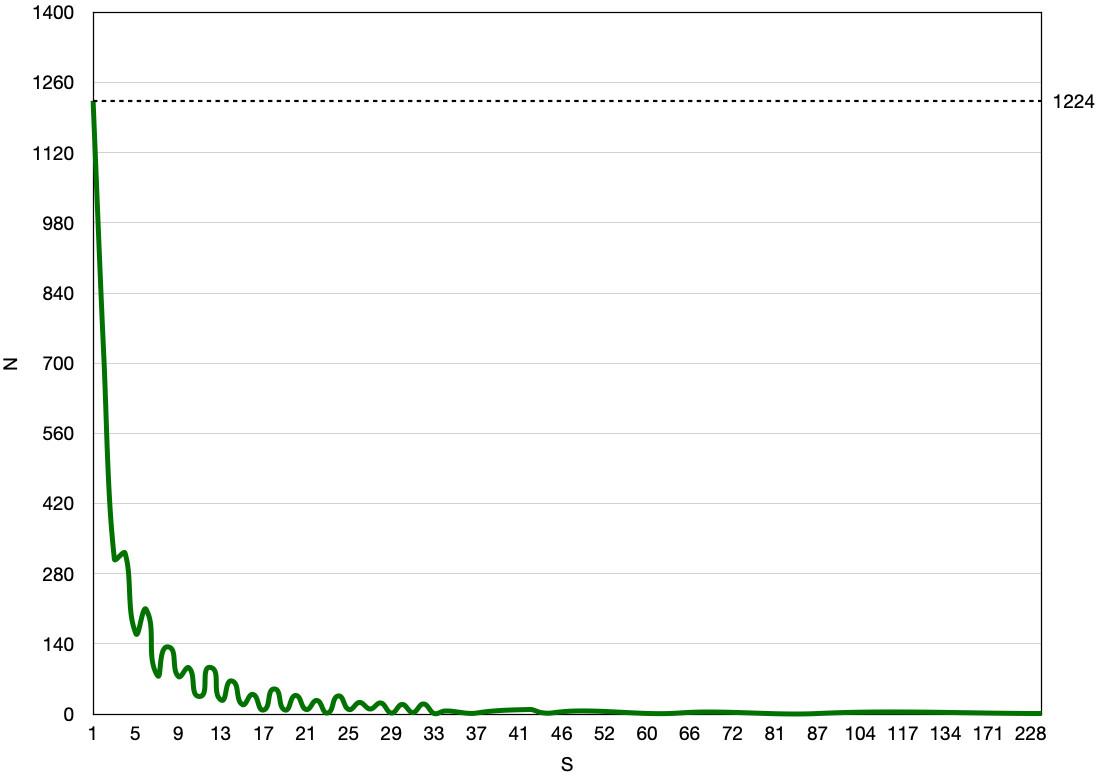
\includegraphics[width=1\linewidth]{./chapter/city/Number_of_cities_having_given_number_of_sister_cities_according_to_Wikidata,_2020.png}%
\caption[Зависимость числа городов от числа имеющихся побратимов, 2020 год.]{Зависимость числа городов всего мира (N) от числа имеющихся у этих городов побратимов (S), 2020 год}%
\label{fig:city_relation_S_N}
\end{marginfigure}

\index{SPARQL!COUNT}
\index{График!LineChart}
\index{SPARQL!SELECT!вложенный}
\begin{lstlisting}[ 
    language=SPARQL, 
    caption={\href{https://w.wiki/pM9}{Число городов с определённым числом побратимов}\protect\footnotemark},
    label=lst:city_relation_S_N,
    xleftmargin=18pt, 
    numbers=left,
    ]
# Count number of cities having sister cities and number of sister cities themselves
#defaultView:LineChart
SELECT ?sisterCount (COUNT(?sisterCount) AS ?FreqNSister) WHERE {                                                                         
	{ # Count sister cities of cities which are ...
		SELECT (COUNT(?sister) AS ?sisterCount) WHERE {        
			VALUES ?cityTypes {wd:Q3957 wd:Q515 wd:Q1549591 wd:Q1637706}
			?city wdt:P31 ?cityTypes. # instances of different types of cities
			?city wdt:P190 ?sister. # with filled property "sister city"
		}
		GROUP BY ?city
	}
}
GROUP BY ?sisterCount # Group by number of sister cities                                     
ORDER BY DESC(?sisterCount) # Order by number of sister cities   
\end{lstlisting}
\footnotetext[17][-52pt]{%
%\footnotetext{
Получено: 90 вариантов числа братских городов в мире в 2020 году. Ссылка на~SPARQL-запрос: \href{https://w.wiki/pM9}{https://w.wiki/pM9}.}

\begin{marginfigure}[8pt]
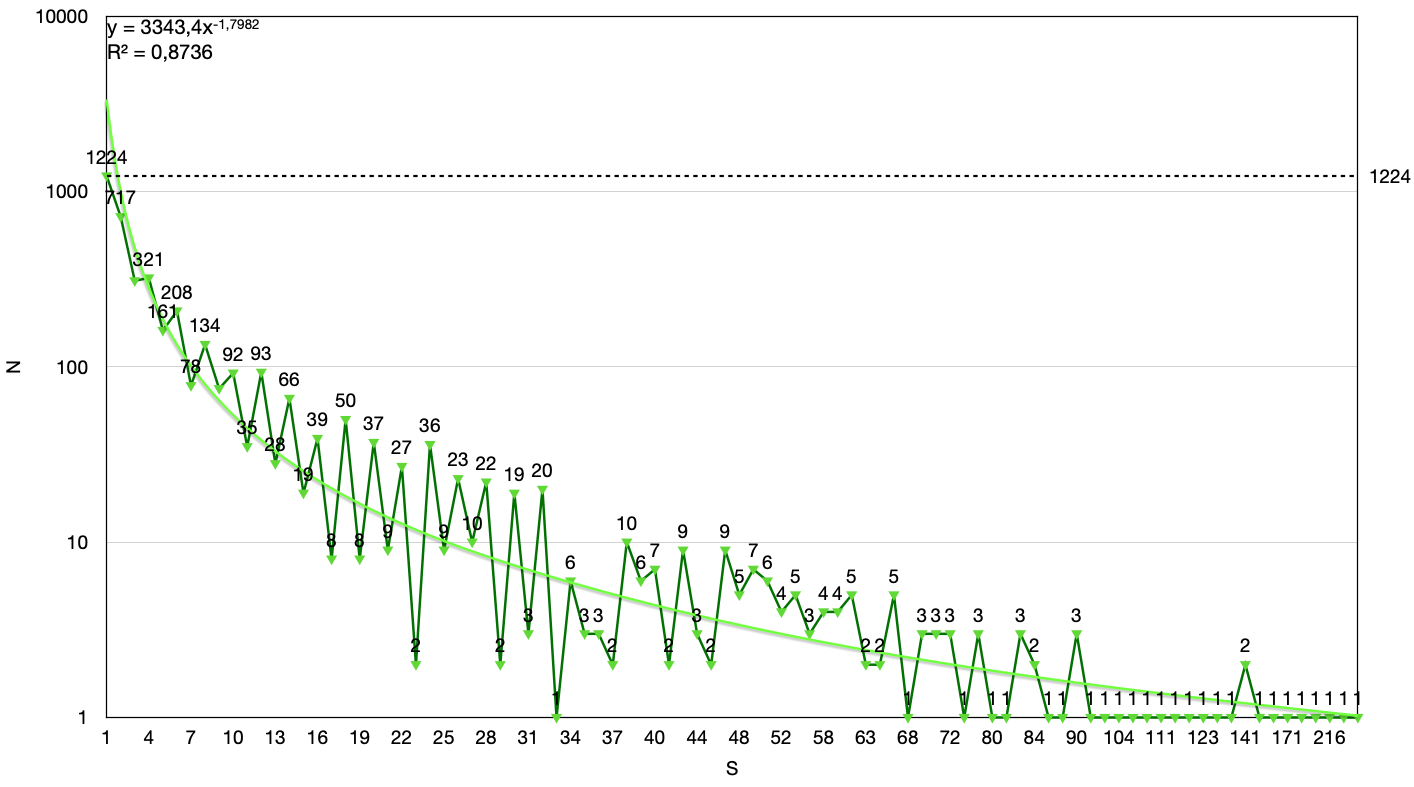
\includegraphics[width=1\linewidth]{./chapter/city/Logarithm_of_the_number_of_cities_having_given_number_of_sister_cities_according_to_Wikidata,_2020.png}%
    \caption[Зависимость числа городов от числа имеющихся побратимов на логарифмической шкале, 2020 год.]
    {Зависимость числа городов мира (N) от числа имеющихся побратимов~(S) на~логарифмической шкале, 2020 год}%
\label{fig:city_ln_relation_S_N}%
\end{marginfigure}

Результаты SPARQL-запроса для всех городов отображены на рис.~\ref{fig:city_relation_S_N}. 
Максимальное значение N (\num{1224} города) наблюдается при S, равном единице, 
затем следует резкое уменьшение числа городов с~увеличением числа имеющихся у них побратимов. 
На рис.~\ref{fig:city_ln_relation_S_N} представлены те же данные, но в~логарифмической шкале. 
Так, чуть более 4 тыс. городов (\num{4046}) побратались хотя~бы с~одним~городом, из~них:
%
\begin{itemize}
\item 32\,\% (\num{1314} городов) связаны братскими отношениями более чем с пятью городами;
\item 18\,\% (728 городов) имеют как минимум 11 городов-побратимов;
\item 9\,\% (345 городов) подружились более чем с 20 городами;
\item 2\,\% (94 города) имеют от 50 побратимов.
\end{itemize}

На основании построенного тренда можно сделать предположение, 
что зависимость числа городов от числа имеющихся у этих городов побратимов 
имеет распределение, близкое к~степенному.

%
%%%%%%%%%%%%%%%% Упражнение 3 %%%%%%%%%%%%%%%%
\marginnote[-12pt]{%
    \MarginQuestion
    Какие из городов были основаны более 400 лет назад: 
    \href{https://w.wiki/oL8}{Москва}, 
    \href{https://w.wiki/oL9}{Саров}, 
    \href{https://w.wiki/oLA}{Казань}, 
    \href{https://w.wiki/oLB}{Астрахань}, 
    \href{https://w.wiki/oLC}{Самара}, 
    \href{https://w.wiki/oLD}{Воронеж}?

См. ответ %~\ref{answer:cities_over_400_age} 
на с.~\pageref{answer:cities_over_400_age}.
}

\index{График!LineChart}
\index{SPARQL!COUNT}
\index{SPARQL!GROUP BY}
\index{SPARQL!AS}
\begin{lstlisting}[ language=SPARQL, 
                    caption={\href{https://w.wiki/pMA}{Число городов России с определённым числом побратимов}\protect\footnotemark},
                    label=lst:city_relation_Russia_S_N,
                    numbers=none
                    ]
#defaultView:LineChart                                                   
# Count No. of cities having sisterCount sister cities  
# and number of sister cities themselves
SELECT ?sisterCount (COUNT(?sisterCount) AS ?FreqNSister) WHERE {                                                                                  
	{ # Count sister cities of cities which are ...
		SELECT (COUNT(?sister) AS ?sisterCount) WHERE {    
			VALUES ?cityTypes {wd:Q3957 wd:Q515 wd:Q1549591 wd:Q1637706}
			?city wdt:P31 ?cityTypes. # instances of different types of cities
			?city wdt:P17 wd:Q159. # belonging to Russia
			?city wdt:P190 ?sister. # with filled property "sister city"
		}
		GROUP BY ?city # Group list by city                             
	}
}
GROUP BY ?sisterCount # Group by number of sister cities
ORDER BY DESC(?sisterCount) # Order by number of sister cities                                  
\end{lstlisting}
\footnotetext[18][-42pt]{Получено: 24 варианта числа братских городов в России в 2020 году. Ссылка на SPARQL-запрос: \href{https://w.wiki/pMA}{https://w.wiki/pMA}.}

Ситуация с отечественными городами представлена на рис.~\ref{fig:city_relation_Russia_S_N}. 
Чуть менее ста городов России (82 города) побратались хотя бы с одним городом, 
из них только 48\,\% (39 городов) связаны братскими отношениями более чем с пятью городами.


\begin{marginfigure}[18pt]
    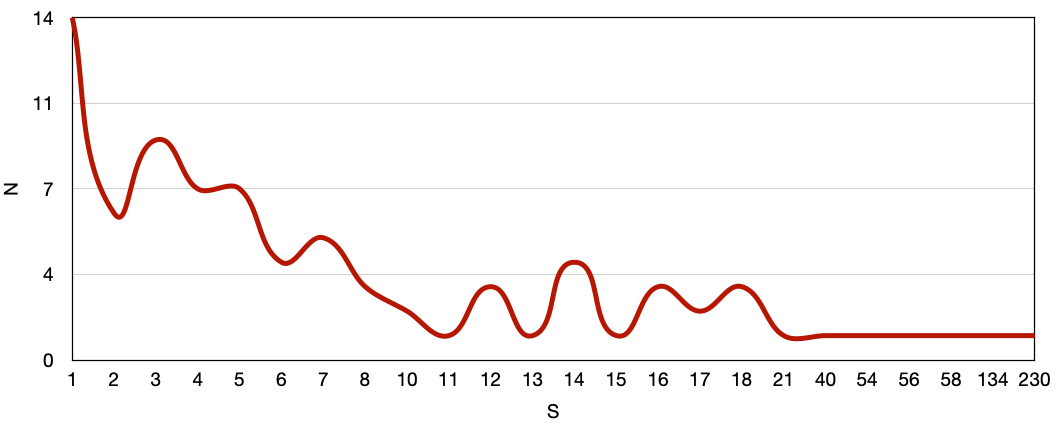
\includegraphics[width=1.0\linewidth]{./chapter/city/Number_of_Russian_cities_having_given_number_of_sister_cities_according_to_Wikidata,_2020.png}
  \caption[Зависимость числа городов России от числа побратимов, 2020 год.]
    {Зависимость числа городов России (N) от числа побратимов (S), 2020 год}
  \label{fig:city_relation_Russia_S_N}
\end{marginfigure}




\newpage
\subsection{У какой страны больше всего побратимов?}

Запрос~\ref{lst:countries_sister_cities} позволяет построить 
пузырьковую диаграмму (рис.~\ref{fig:Bubble_countries_sister_cities}), 
показывающую соотношение количества городов-побратимов между странами.

\index{График!BubbleChart}
\index{SPARQL!GROUP BY}
\index{SPARQL!ORDER BY!DESC}

\begin{lstlisting}[ language=SPARQL, 
                    caption={\href{https://w.wiki/5At7}{Пузырьковая диаграмма стран мира, упорядоченных по количеству городов-побратимов}\protect\footnotemark},
                    label=lst:countries_sister_cities,
                    numbers=none,
                    ]
#defaultView:BubbleChart
# Ordered list of countries by number of sister cities
SELECT DISTINCT ?country ?countryLabel (COUNT(?sister) as ?sisterCount) WHERE
{ VALUES ?cityTypes {wd:Q3957 wd:Q515 wd:Q1549591 wd:Q1637706}
  ?city wdt:P31 ?cityTypes;    # instance of some type of city
        wdt:P17 ?country;      # belongs to country
        wdt:P190 ?sister.      # has a sister city
  SERVICE wikibase:label {bd:serviceParam wikibase:language "ru"}
}
GROUP BY ?country ?countryLabel
ORDER BY DESC(?sisterCount)
\end{lstlisting}
\footnotetext[19][-6.1cm]{Получено: 208 стран в 2020 году. Ссылка на SPARQL-запрос: \href{https://w.wiki/5At7}{https://w.wiki/5At7}.}


\begin{marginfigure}[-1.5cm]
%{
%\setlength{\fboxsep}{0pt}%
%\setlength{\fboxrule}{1pt}%
%\fcolorbox{gray}{gray}{
    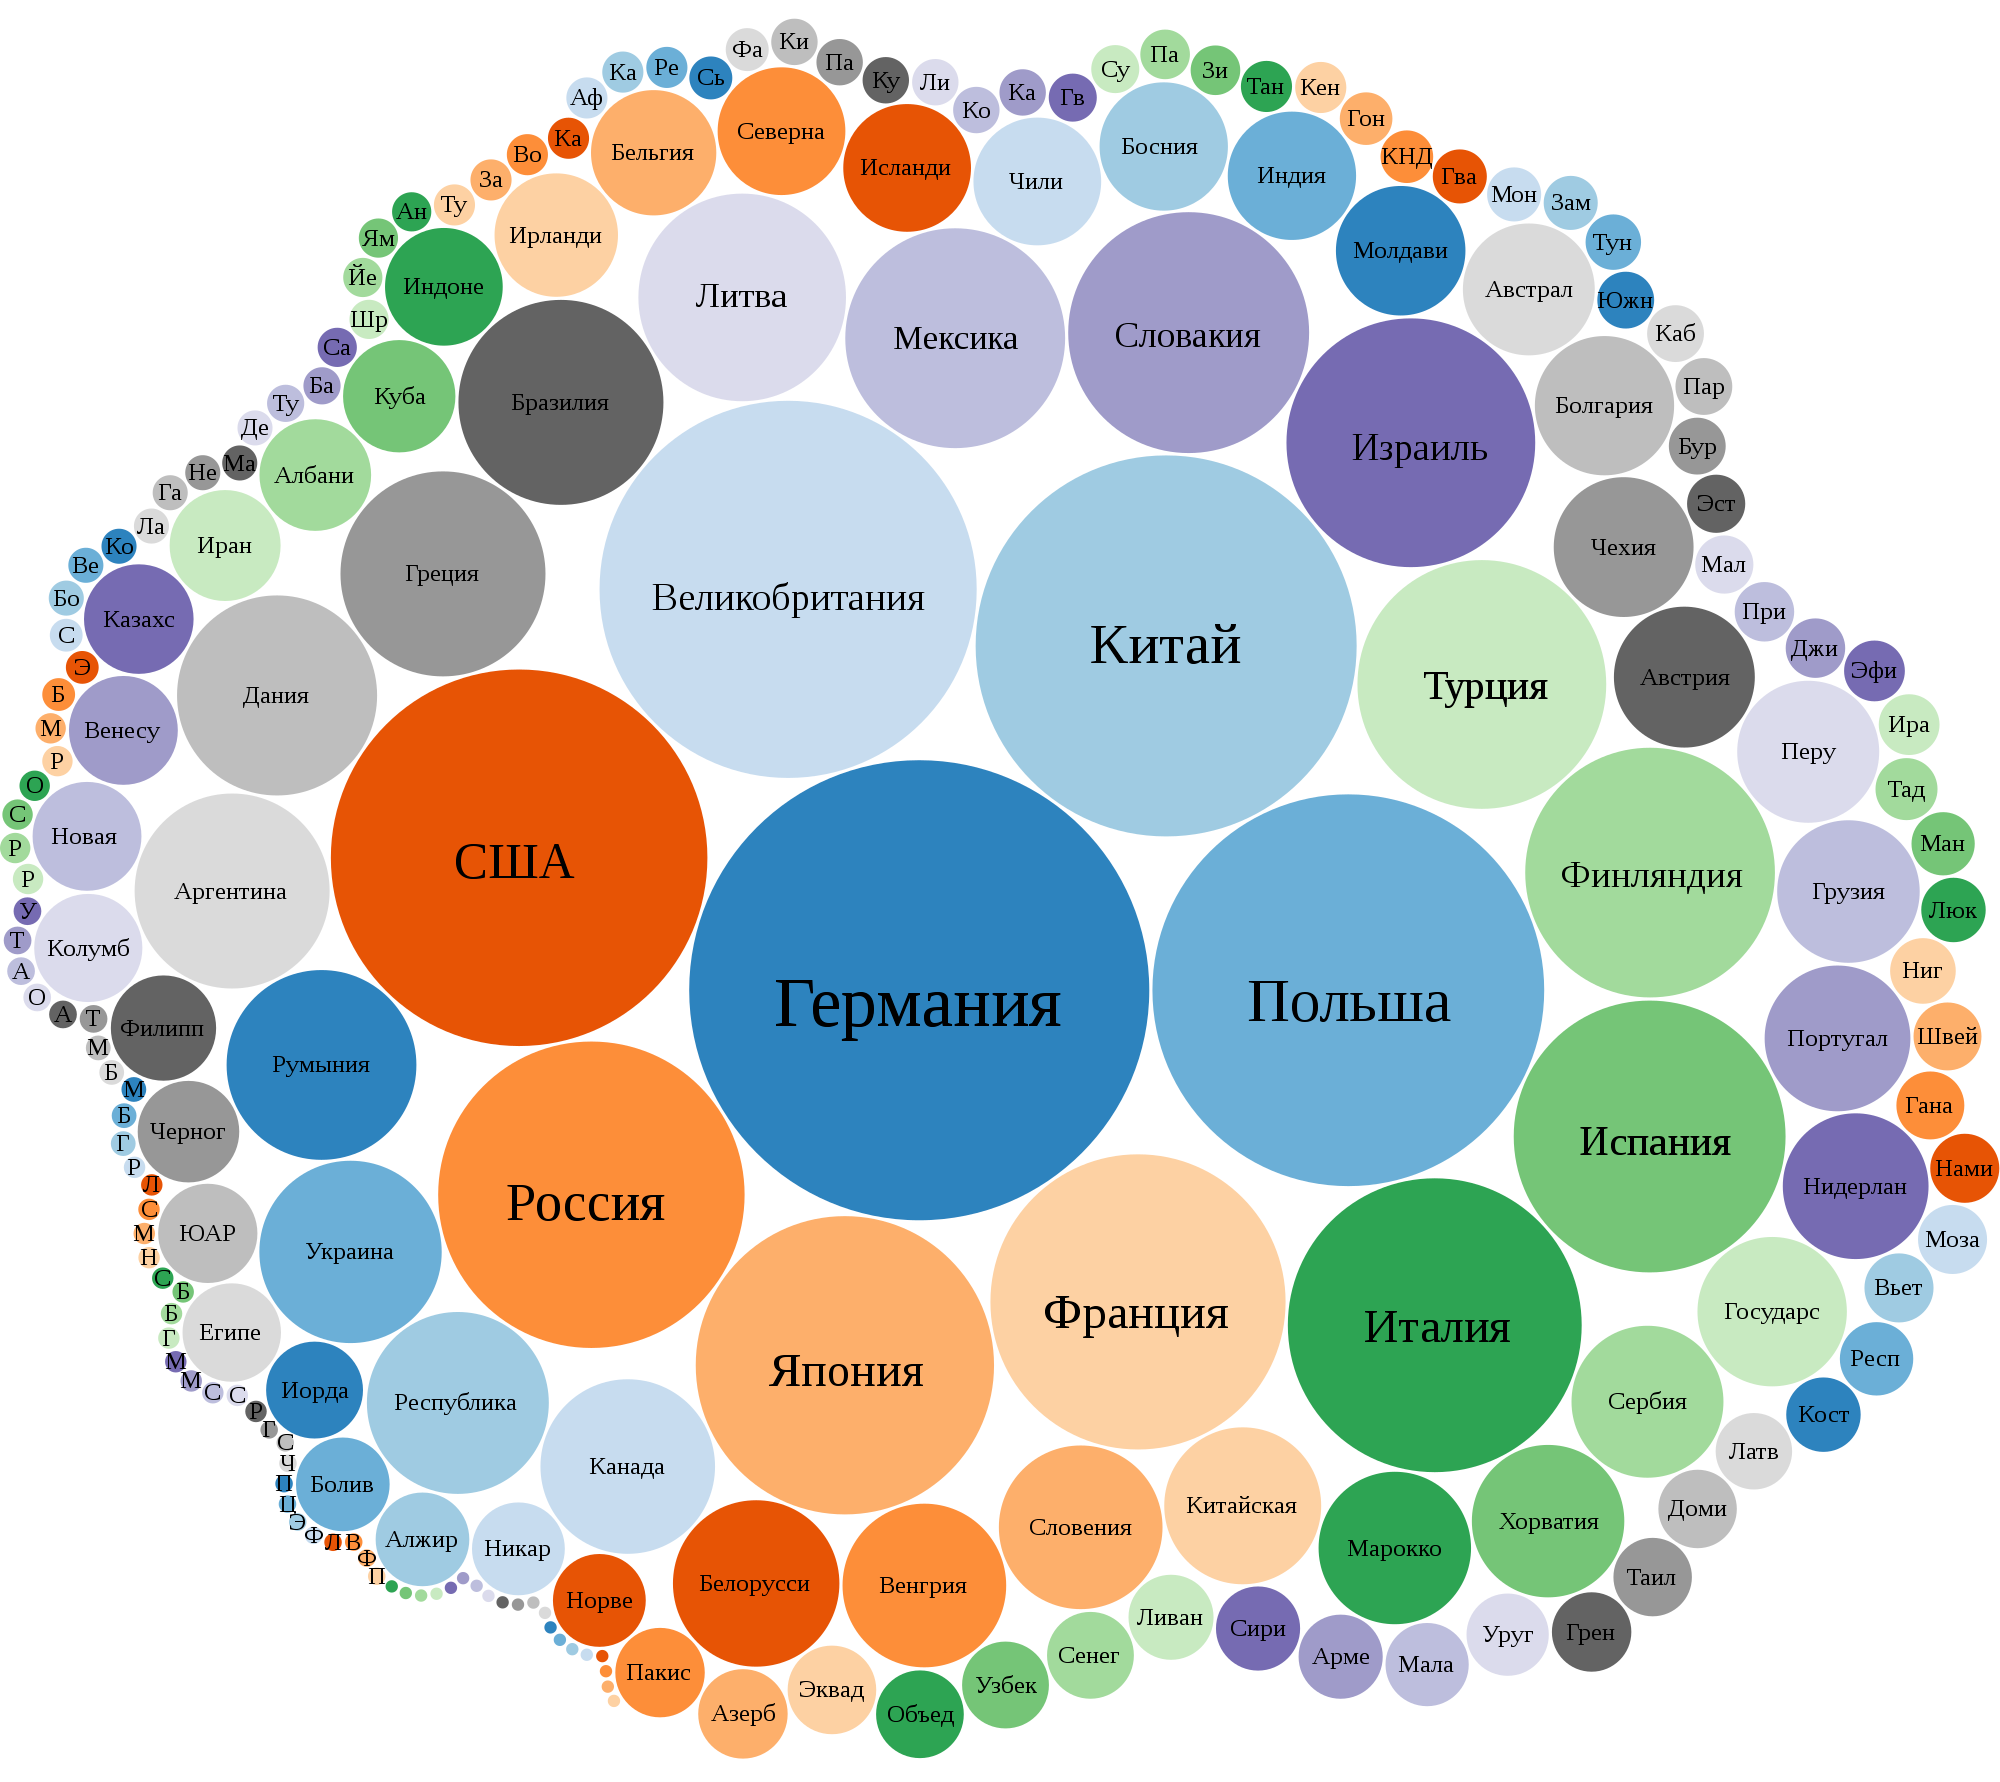
\includegraphics[width=\linewidth]{./chapter/city/Bubble_chart_number_of_sister_cities_of_countries_according_to_Wikidata,_2020_(RU).png}
%}%
%}
\caption[Пузырьковая диаграмма стран мира по числу побратимов у городов, 2020 год.]
    {Пузырьковая диаграмма стран мира по числу побратимов у городов страны, 2020 год}%
  \label{fig:Bubble_countries_sister_cities}%
\end{marginfigure}



% # List of countries that have sister cities with cities in Germany
\index{SPARQL!COUNT}
\index{SPARQL!DISTINCT}
\index{SPARQL!GROUP BY}
\index{SPARQL!ORDER BY!DESC}
\index{SPARQL!VALUES}
\begin{lstlisting}[ language=SPARQL, 
                    caption={\href{https://w.wiki/5As4}{Список стран, имеющих города-побратимы с городами Германии}\protect\footnotemark},
                    label=lst:sister_cities_with_Germany,
                    numbers=none,
                    ]
SELECT ?country ?countryLabel (COUNT(DISTINCT ?sister) as ?sisterCount) WHERE
{ VALUES ?cityTypes {wd:Q3957 wd:Q515 wd:Q1549591 wd:Q1637706}
  ?city wdt:P31 ?cityTypes; # instance of one of the city types
        wdt:P17 wd:Q183;    # belongs to Germany
        wdt:P190 ?sister.   # has a sister city
  ?sister wdt:P17 ?country. # sister city belongs to some country
  SERVICE wikibase:label { bd:serviceParam wikibase:language "ru" }
}
GROUP BY ?country ?countryLabel
ORDER BY DESC(?sisterCount)\end{lstlisting}%
\footnotetext{Получено: 93 страны в 2020 году и~100~стран в~2022~году. 
              На первом месте находится Франция, у неё 268 городов, имеющих побратимов в Германии в 2022 году. 
              SPARQL-запрос: \href{https://w.wiki/5As4}{https://w.wiki/5As4}.}


На пузырьковой диаграмме (рис.~\ref{fig:Bubble_countries_sister_cities}) 
размер шарика соответствует числу побратимов у городов страны. 
На 2020 год больше всего побратимов имела Германия (\num{1375} городов). 
В~2022 году у~Германии было уже 1703 побратима, 
а~на~первое место вышел Китай с 2542 побратимами. 
Полный список стран, с которыми Германия имеет города-побратимы, 
можно получить с помощью запроса~\ref{lst:sister_cities_with_Germany}.

В~табл.~\ref{tab:germany_sister_cities} приведен список из первых 10 стран, 
имеющих наибольшее количество побратимов с~городами Германии на 2020 и 2022 годы. 




\subsection{Ближайшие соседи России по числу городов-побратимов}

%% Но эта таблица из предыдущего раздела, для оформления перенесена сюда
\begin{margintable} 
    \vspace{14pt}
    \caption[Страны с наибольшим числом побратимов с городами Германии, 2020 год.]
    {Страны с наибольшим числом побратимов из Германии,\\2020 и 2022 годы}
%   {Количество городов-побратимов в различных странах\\с городами Германии на 2020 и 2022 годы\vspace{3pt}}
    \label{tab:germany_sister_cities}
%  \centering
%\raggedright
%  \fontfamily{ppl}\selectfont
  \begin{tabular}{| c | l | c | c |}
\hline%\toprule
%\textnumero & \multicolumn{1}{ c |}{Название страны} & \multicolumn{1}{p{0.3\textwidth} |}{\centering Количество городов-побратимов} & \multicolumn{1}{p{0.2\textwidth} |}{\centering \% от общего числа} \\
\textnumero & Страна            & 2020 & 2022 \\ \hline% \midrule
1 & \wdqName{Франция}{142}      & 247  & 268 \\
2 & \wdqName{Германия}{183}     & 195 & 204 \\
3 & \wdqName{Великобритания}{145} & 120 & 125 \\
4 & \wdqName{Италия}{38}        & 86 & 91  \\
5 & \wdqName{Польша}{36}        & 81 & 83  \\
6 & \wdqName{США}{30}           & 60 & 63  \\
7 & \wdqName{Австрия}{40}       & 41 & 42  \\
8 & \wdqName{Россия}{159}       & 39 & 42  \\
9 & \wdqName{Венгрия}{28}       & 39 & 41  \\
10 & \wdqName{Бельгия}{31}      & 33 & 32  \\ \hline
\end{tabular}
%    \bottomrule  \end{tabular}%
\end{margintable}
%
%
%
%
Запрос~\ref{lst:countries_sister_cities_with_Russia} позволяет получить список стран, 
с которыми у России есть города-побратимы. 
Результаты запроса представлены на рис.~\ref{fig:Map_closest_neighbours_Russia}.
%
%%%%%%%%%%%%%%%% Упражнение 2 %%%%%%%%%%%%%%%%
\marginnote[5\baselineskip]{%
    \MarginQuestion
    Какому городу России принадлежит этот флаг?
    \vspace{5pt}

%\begin{marginfigure}[0.0cm]
\includegraphics[width=5cm]{./chapter/city/Flag_of_Karabulak_(Ingushetia).png}%

\vspace{2pt}
См. ответ %~\ref{answer:cities_flags} 
на~с.~\pageref{answer:cities_flags}.
%  \caption{Какому городу России принадлежит этот флаг?\\См. ответ~\ref{answer:cities_flags} на~с.~\pageref{answer:cities_flags}.}
%  \label{fig:flag_question_city}%
%\end{marginfigure}
}

У России нашлось больше двадцати городов-побратимов с такими странами, 
как США~(46), Китай~(46), Германия (44), Украина (28), Болгария (25), 
Польша (24), Франция (23) и~Италия~(22).


\index{SPARQL!COUNT}
\index{SPARQL!NOT IN}
\index{SPARQL!FILTER}
\index{SPARQL!OPTIONAL}
\index{SPARQL!BIND}
\index{SPARQL!IF}
\index{График!Map}
\begin{lstlisting}[ language=SPARQL, 
                    caption={\href{https://w.wiki/q5Z}{Ближайшие соседи России по числу побратимов}\protect\footnotemark},
                    label=lst:countries_sister_cities_with_Russia,
                    numbers=none,
                    ]
#defaultView:Map
SELECT ?country ?countryLabel ?sisterCount ?shape ?layer WHERE {
  { 
    SELECT ?country ?countryLabel (COUNT(DISTINCT ?sister) as ?sisterCount) 
    WHERE {  
        VALUES ?cityTypes {wd:Q3957 wd:Q515 wd:Q1549591 wd:Q1637706}
        ?city wdt:P31 ?cityTypes.   # instances of different types of cities
        ?city wdt:P17 wd:Q159.      # city belongs to Russia
        ?city wdt:P190 ?sister.     # city has "sister city"
        ?sister wdt:P17 ?country.   # which belongs to "country"
        FILTER(?country NOT IN(wd:Q159)) # except the Russia
        SERVICE wikibase:label { bd:serviceParam wikibase:language "ru" }
    }
    GROUP BY ?country ?countryLabel
    ORDER BY DESC(?sisterCount)
  }
  OPTIONAL {?country wdt:P3896 ?shape.} # country has "geoshape"
  BIND(
	    IF(?sisterCount < 5, "<5",
		IF(?sisterCount <= 10, "5-10",
		IF(?sisterCount <= 20, "11-20",
		IF(?sisterCount <= 30, "21-30",
		IF(?sisterCount <= 40, "31-40",
		">40"))))) AS ?layer).
}
\end{lstlisting}
\footnotetext{Получено: 102 страны в 2020 году. Ссылка на SPARQL-запрос: \href{https://w.wiki/q5Z}{https://w.wiki/q5Z}.}

\begin{figure*}
{
\setlength{\fboxsep}{0pt}%
\setlength{\fboxrule}{1pt}%
\fcolorbox{gray}{gray}{\includegraphics[width=0.96\linewidth]{./chapter/city/Map_of_closest_neighbours_of_Russia_by_number_of_sister_cities,_2020.png}}
}
	\caption{Карта ближайших соседей России по числу городов-побратимов,\\2020 год}
	\label{fig:Map_closest_neighbours_Russia}
\end{figure*}







%%%%%%%%%%%%%%%%%%%%%%%%%%%%%%%%%%%%%%%%%%%%%%%%%%%%%%%
\section{Полнота и недостатки Викиданных: дублирование объектов}
\label{sect:city-completness}

Городом принято называть крупный населённый пункт, 
жители которого, как правило, не заняты сельским хозяйством. 
При этом разные страны используют различные критерии 
при наделении поселений статусом города, 
основным из которых является численность населения\marginnote{%
%
    \MarginInternalLink
    Вопрос отнесения населённого пункта к сельскому или городскому типу также решается 
    в~подразделе <<\nameref{sec:list-village-city-types-in-Russia}>> на с.~\pageref{sec:list-village-city-types-in-Russia}.
%
}. 
Некоторые страны и вовсе не применяют понятие города. 
Так, во Франции используется только одна географическая единица подобного рода~--- коммуна, 
вне зависимости от количества проживающих в ней людей и рода их деятельности. 
Поэтому чётко определить, какой населённый пункт относить к~городам, а~какой~нет, 
может быть затруднительно.

На практике некоторые объекты Викиданных могут одновременно являться экземплярами городов разных типов. 
Например, \wdqName{Шанхай}{8686} отнесен к трём исследуемым объектам: 
\wdqName{city}{515}, \wdqName{big city}{1549591}, \wdqName{city with millions of inhabitants}{1637706}. 
Такое множественное присваивание влияет на результаты SPARQL-запросов. 
Например, 
при~использовании конструкции \href{https://en.wikibooks.org/wiki/SPARQL/UNION}{UNION}\footnote[][-15pt]{%
%
    \index{SPARQL!UNION}
    Более подробно о~команде~\texttt{UNION} 
    см.~в~Английском Викиучебнике SPARQL по~ссылке: \href{https://en.wikibooks.org/wiki/SPARQL/UNION}{https://en.wikibooks.org/wiki/SPARQL/UNION}.%
} %
в~результатах запроса~\ref{lst:different_city_types} 
объект \lstinline|Шанхай| встречается три раза вместо одного. 

\index{SPARQL!Свойство!subclass of}
Викиданные имеют механизм наследования, 
выражающийся в свойстве \href{https://www.wikidata.org/wiki/Property:P279}{subclass of}. 
Заключается этот механизм в том, что если объект является экземпляром\, \lstinline{big city}, 
то он является и экземпляром объекта \lstinline{city}, 
так как\, \lstinline|big city|~--- это~подкласс~\lstinline|city|. 
Таким образом, описанную выше ситуацию с~\lstinline|Шанхаем| можно разрешить, 
оставив только один класс, например\, \mbox{\lstinline{city with millions of inhabitants}}. 
Стоит отметить, что замена конструкции 
с~использованием \lstinline|UNION| (запрос~\ref{lst:example_union_city}) 
на конструкцию с учётом подклассов (запрос~\ref{lst:example_subclasses_city})
неэквивалентна. 
Рассмотренный ранее \lstinline|Шанхай| встречается в новой выборке даже четыре раза. 
Дело в том, что, помимо части исследуемых классов, есть и другие классы, наследуемые от~\lstinline|city|. 
Например, \wdqName{lost city}{2974842}, 
\wdqName{free imperial city}{57318}, 
\wdqName{autonomous city}{1094397} и даже \wdqName{ideal city}{1656724}.

\begin{lstlisting}[ language=SPARQL, 
                    caption={\href{https://w.wiki/k5T}{Пример использования конструкции UNION}\protect\footnotemark},
                    label=lst:example_union_city,
                    numbers=none,
                    ]
SELECT ?city ?cityLabel WHERE {
    { ?city wdt:P31 wd:Q515 } UNION     # instances of "city"            
    { ?city wdt:P31 wd:Q1549591 } UNION # OR instances of "big city"               
    { ?city wdt:P31 wd:Q1637706 }       # OR instances of "city 1000000+"
    SERVICE wikibase:label { bd:serviceParam wikibase:language "ru" }
}
\end{lstlisting}
\footnotetext{Ссылка на SPARQL-запрос: \href{https://w.wiki/k5T}{https://w.wiki/k5T}.}




\newpage
\begin{lstlisting}[ language=SPARQL, 
                    caption={\href{https://w.wiki/jyB}{Пример использования конструкции с подклассами}\protect\footnotemark},
                    label=lst:example_subclasses_city,
                    numbers=none,
                    ]
SELECT ?city ?cityLabel WHERE {
    ?city wdt:P31/wdt:P279* wd:Q515 # instances of city subclasses
    SERVICE wikibase:label { bd:serviceParam wikibase:language "ru" }
}
\end{lstlisting}
\footnotetext{Ссылка на SPARQL-запрос: \href{https://w.wiki/jyB}{https://w.wiki/jyB}.}

Вероятно, в связи с неоднозначностью критериев присвоения статуса города 
были созданы подклассы для конкретных стран~--- это \wdqName{city in Chile}{25412763}, 
\wdqName{city in Cyprus}{29556224}, \wdqName{city of Japan}{494721} и т.~д. 
Не обошла стороной эта тенденция и города России: 
существует объект Викиданных <<Городское поселение в России>>\sidenote{%
    %
    По~табл.~\ref{tab:human-settlement-Russia} на~с.~\pageref{tab:human-settlement-Russia} видно, 
    что 
    \wdqName{urban settlement in Russia}{2661988} и \wdqName{city or town}{7930989} 
    являются наиболее многочисленными объектами-городами в~России.%
}.


По данным переписи населения России 2010 года\sidenote{% \autocite{city_perepis_2010}
%
    Число районов, городских и сельских населенных пунктов по субъектам Российской Федерации. 
    Всероссийская перепись населения 2010 года. 
    URL: \href{https://bit.ly/2JPL34b}
              {https://bit.ly/2JPL34b}. 
%
} % eo sidenote
и переписи населения Крыма 2014 года\sidenote{%   \autocite{city_perepis_2014}
%
    Итоги переписи населения в Крымском федеральном округе. 
    Федеральная служба государственной статистики. 2015. 
    URL: \href{https://bit.ly/2Lflc6F}
              {https://bit.ly/2Lflc6F}. 
%             
}, число городов составило соответственно 1100 и 17. 
Все города России перечислены на~страницах 
как Русской 
    (см.~<<\href{https://ru.wikipedia.org/?curid=951219}{Список городов России}>>), 
так и Английской Википедии 
    (см.~``\href{https://en.wikipedia.org/?curid=171916}{List of cities and towns in Russia}'').
С~другой стороны, Викиданные содержат 1108 российских городов на~2024 год\sidenote{%
%   
    Ссылка на SPARQL-запрос для подсчёта числа российских городов:
    \href{https://w.wiki/jyP}
         {https://w.wiki/jyP}.
%
}. То есть Викиданные почти полностью покрывают российские города. 

%%%%%%%%%%%%%%%%%%%%%%%%%%%%%%%%%%%%%%%%%%%%%%%%%%%%%%%
\section{Упражнения}

\begin{enumerate}
\item Постройте граф братских городов России.
\item Получите список городов России, находящихся за полярным кругом.
\item На какой реке в России стоит наибольшее число городов?
\item У какой страны самая большая доля городов-побратимов внутри страны относительно числа побратимов, которые связывают эту страну с другими странами?
\end{enumerate}

\chapter{Анализ стран: возраст, формы правления и этнохоронимы}
\label{ch:country}

Глава посвящена исследованию стран на основе Викиданных. 
С помощью SPARQL-запросов, вычисляемых на объектах <<страна>>, получены: 
список современных стран, перечень всех стран, упорядоченных по дате создания, 
список этнохоронимов стран. 
Построены пузырьковая диаграмма с формами правления стран, 
граф соседних стран и карта соседних стран России. 
Выполнена оценка Викиданных по количеству исторических и~современных стран, 
по количеству заполненных этнохоронимов у~стран. 
%%%%%%%%%%%%%%%%%%%%%%%%%%%%%%%%%%%%%%%%%%%%%%%%%%%%%%%


\begin{marginfigure}[7\baselineskip]
%\setlength{\fboxsep}{0pt}%
%\setlength{\fboxrule}{1pt}%
%\fcolorbox{gray}{gray}{
    \includegraphics[width=0.8\linewidth]{chapter/country/ProWD_country.png}
    \caption{Индекс Джини~--- равномерность заполнения свойств <<стран>>, 2020 год}
% deadlink \href{https://prowd.id/dashboards/86b6f91a8131/profile}{ProWD.id}, 2020 год.\\
	\label{fig:ProWD_country}%
\end{marginfigure}


\section{Список стран и степень полноты информации ряда стран}

\index{Коэффициент Джини}
Анализ экземпляров объекта \wdqName{страна}{6256} 
с~помощью сервиса ProWD в~2020 году показал, 
что индекс Джини равен 0.091 (рис.~\ref{fig:ProWD_country}). 
Это значит, что страны хорошо проработаны в~Викиданных 
и~имеют примерно одинаковое количество заполненных свойств (рис.~\ref{fig:ProWD_country}). 
Легко убедиться, что это достаточно большое количество свойств. 

Построим список всех стран на английском и русском языках (запрос~\ref{lst:country}).

\begin{lstlisting}[ language=SPARQL, 
    caption={\href{https://w.wiki/k6L}{Экземпляры объекта <<страна>>}\protect\footnotemark},
    label=lst:country, 
    numbers=none,
]
#List of countries in English and Russian
SELECT ?country ?label_en ?label_ru WHERE
{
		?country wdt:P31 wd:Q6256. # instance of country
		?country rdfs:label ?label_en filter (lang(?label_en) = "en").
		?country rdfs:label ?label_ru filter (lang(?label_ru) = "ru").
}
\end{lstlisting}
\footnotetext[1][0cm]{Получено: 205 стран на 2017 год и 175 стран на 2020 год. Ссылка на SPARQL-запрос: \href{https://w.wiki/k6L}{https://w.wiki/k6L}.}

%По степени заполненности свойств на Викиданнных можно различать <<полные>> и  <<пустые>> страны. 
%
%Примерами наиболее полных и проработанных стран на Викиданных по данным ProWD\autocite{prowd_balakireva} являются: \wdqName{Израиль}{801} (127 свойств), \wdqName{Франция}{142} (126 свойств), \wdqName{Соединённые Штаты Америки}{30} (124 свойства).
%
%Наименьшее количество свойств у \wdqName{Соединённых провинций Центральной Америки}{8842993} (3 свойства) и \wdqName{Джалаириды}{8842993} (9 свойств).



%%%%%%%%%%%%%%%%%%%%%%%%%%%%%%%%%%%%%%%%%%%%%%%%%%%%%%%
\section{Возраст стран и почему Россия бывает не страной? О конструкции p:/ps:}
\label{ch:RussiaNotCountryPPS}


%%%%%%%%%%%%%%%% Упражнение 2 %%%%%%%%%%%%%%%%
\marginnote{%
    \MarginQuestion
%	Какое количество административных единиц имеют следующие страны:
	У \href{https://w.wiki/mzN}{Латвии} их 119, у \href{https://w.wiki/mzP}{Таиланда} 77, 
    у \href{https://w.wiki/mzR}{Дании} 5, а у \href{https://w.wiki/myt}{России} 81.\\ 
    О~количестве чего идет речь?
	\begin{itemize}
		\item Количество городов с населением более миллиона человек
		\item Количество высших учебных заведений
		\item Количество административных единиц
		\item Количество официальных языков
	\end{itemize}
	См. ответ %~\ref{answer:administrative_territorial} 
    на с.~\pageref{answer:administrative_territorial}.
}

Построим список стран, отсортированных по дате основания, 
то есть по первому упоминанию о~ней (запрос~\ref{lst:age_of_country}).

\begin{lstlisting}[ language=SPARQL, 
    caption={\href{https://w.wiki/suP}{Даты основания стран}\protect\footnotemark},
    label=lst:age_of_country, 
    numbers=none,
]
# List of countries sorted by inception 
SELECT ?country ?countryLabel ?inception
WHERE
{
	?country wdt:P31 wd:Q6256.    # instance of country
	?country wdt:P571 ?inception. # the first mention
	SERVICE wikibase:label { bd:serviceParam wikibase:language "ru" }
}
ORDER BY (?inception)
\end{lstlisting}
\footnotetext{Получено: 112 стран на 2017 год и 199 стран на 2020. Ссылка на SPARQL-запрос: \href{https://w.wiki/suP}{https://w.wiki/suP}.}

В результате выполнения запроса~\ref{lst:age_of_country} 
получен скромный список, включающий на 2020 год всего 199 стран. 
На примере России разберёмся, в чём здесь дело. 
Объект \wdqName{Россия}{159} в~поле \mbox{\lstinline|instance of|} содержит не одно, а восемь значений, в том числе \wdqName{country}{6256}.

Решение и ответ на этот вопрос были найдены на странице Wikidata:Request a query%
\sidenote{%
    На странице Викиданных ``\href{https://w.wiki/LX}{Request a query}'' 
    одни редакторы задают вопросы, как написать тот или иной скрипт, 
    а~другие редакторы им отвечают. Пользуйтесь этим форумом. 
    Вот ссылка с~ответом на~наш вопрос на~этом форуме: 
    \href{https://w.wiki/tLm}{https://w.wiki/tLm}, 
    см.~раздел ``List of countries''.%
%
}. Дело~в~том, что конструкция wdt позволяет находить только истинные значения. 
Для~России предпочтительным ответом (англ. preferred value) 
\index{SPARQL!Preferred value}
в~поле\, \lstinline|instance of| указано <<суверенное государство>>, а не <<страна>>. 
Чтобы проверить все варианты, представленные в поле \lstinline|instance of| России, 
нужно использовать конструкцию \lstinline|p:/ps:|.

Таким образом, запрос~\ref{lst:list_of_country_instance_of} 
позволяет получить больше стран, отсортированных по дате создания. 
В~2020 году было получено 235~стран, в 2022~--- 246~стран.


\newpage
\begin{lstlisting}[ language=SPARQL, 
    caption={\href{https://w.wiki/5BCN}{Список стран, отсортированных по дате основания}\protect\footnotemark},
    label=lst:list_of_country_instance_of, 
    numbers=none,
]
# List of countries sorted by inception date
SELECT ?country ?countryLabel (MIN(?year) AS ?min_year) WHERE
{
    ?country p:P31  [ps:P31 wd:Q6256];      # instance of a country 
             p:P571 [ps:P571 ?inception].   # all inception dates
    BIND(YEAR(?inception) AS ?year)
    SERVICE wikibase:label { bd:serviceParam wikibase:language "ru" }
}
GROUP BY ?country ?countryLabel
ORDER BY ?min_year
\end{lstlisting}
\footnotetext{Получено: 235 стран в~2020 году и 246~стран в~2022~году. Ссылка на SPARQL-запрос: \href{https://w.wiki/5BCN}{https://w.wiki/5BCN}.}

Чтобы убрать из этого списка уже не существующие страны, 
то есть экземпляры объекта \wdqName{historical country}{3024240}, 
используем оператор \lstinline|MINUS|. 
С помощью запроса~\ref{lst:list_of_country_instance_of_} получим список действующих, 
то есть неисторических, стран с известной датой основания.

\begin{lstlisting}[ language=SPARQL, 
    caption={\href{https://w.wiki/5BCP}{Список стран, отсортированных по дате основания, не включающий исторические страны}\protect\footnotemark},
    label=lst:list_of_country_instance_of_, 
    numbers=none,
]
# List of countries sorted by inception date without historical countries
SELECT ?country ?countryLabel (MIN(?year) AS ?min_year) WHERE
{
	?country p:P31 [ps:P31 wd:Q6256].               # instance of a country 
	MINUS {?country p:P31 [ps:P31 wd:Q3024240]}.    # except historical countries
	?country p:P571 [ps:P571 ?inception].           # all inception dates
	BIND(YEAR(?inception) AS ?year)
	SERVICE wikibase:label { bd:serviceParam wikibase:language "ru" }
}
GROUP BY ?country ?countryLabel
ORDER BY ?min_year
\end{lstlisting}

\footnotetext{Получено: 211 стран в 2020 году и 212 стран в 2022 году. Ссылка на~SPARQL-запрос: \href{https://w.wiki/5BCP}{https://w.wiki/5BCP}.}

Например, первое упоминание о~\wdqName{Франции}{142} было в~463~году, 
о~\wdqName{России}{159}~--- в~862-м, 
о~\wdqName{Республике~Косово}{1246}~--- в~2008-м, 
о~\wdqName{Южном~Судане}{958}~--- в~2011~году. 
Наибольшее количество стран появилось в 1960 году (16 стран), 
в 1991-м (15 стран), в~1962-м (6~стран) и в~1821~году (6~стран).


\newpage
Выведем список стран с пустым свойством <<дата основания>> (листинг~\ref{lst:without_inception}). 
Такие некомплектные объекты Викиданных могли быть созданы по ошибке или могут содержать какие-то дефекты. 
Можно посмотреть историю правок объекта и обратиться с~вопросом к~редакторам этой статьи. 
Подробнее о~том, что такое <<история правок>> в~вики-проектах 
и как~с~ней работать см. в~учебнике\sidenote{\fullcite{Krizhanovsky2015}.}.

\begin{lstlisting}[ language=SPARQL, 
    caption={\href{https://w.wiki/k6q}{Страны с незаполненной датой основания}\protect\footnotemark},
    label=lst:without_inception,
    numbers=none,
]
#List of `instances of` "countries without a inception" 
SELECT ?country ?countryLabel WHERE
{
    ?country wdt:P31 wd:Q6256.      # instance of country
    MINUS { ?country wdt:P571 [] }. # inception of country is empty
    SERVICE wikibase:label { bd:serviceParam wikibase:language "ru" }
}
\end{lstlisting}
\footnotetext{Получено: 100 стран на 2017 год и 7 стран на 2020 год. Ссылка на~SPARQL-запрос: \href{https://w.wiki/k6q}{https://w.wiki/k6q}.}




\subsection{Объём Викиданных по современным и историческим странам}

Проанализируем полноту Викиданных на примере исторических и~современных стран. 
По данным <<Общероссийского классификатора стран мира>> 
на Земле существует 253~страны\sidenote{%
%
    URL: \href{https://classifikators.ru/oksm}
                  {https://classifikators.ru/oksm}.%
%
}.\, % eo sidenote
Авторы статьи Википедии 
<<\href{https://ru.wikipedia.org/?curid=52627}{Список государств}>> 
не~смогли указать какое-то одно число. 
Статья Английской Вики\-педии 
``\href{https://en.wikipedia.org/?curid=68253}{List of sovereign states}'' 
содержит список из~205 стран. 

Отдельного анализа заслуживают древние, уже не существующие государства, 
например \wdqName{Ассирия}{41137}. 
Объекты таких стран на Викиданных являются экземплярами не~объекта country, 
а~объекта historical country (историческая страна). 
%
С помощью запроса~\ref{lst:List_of_historical_countries} построим список исторических государств. 
Таких бывших государств на 2020 год оказалось 3~тыс., что на порядок больше числа современных государств.
%
%%%%%%%%%%%%%%%% Упражнение 2 %%%%%%%%%%%%%%%%
\marginnote{%
    \MarginQuestion
    %	Какое количество административных единиц имеют следующие страны:
    Напишите запрос, чтобы найти государства, существовавшие дольше всех.\\
    См. ответ %~\ref{answer:old_countries} 
    на с.~\pageref{answer:old_countries}.
}


\index{SPARQL!p:[ps:]!instance of}
\begin{lstlisting}[ language=SPARQL, 
    caption={\href{https://w.wiki/tQN}{Список исторических стран}\protect\footnotemark},
    label=lst:List_of_historical_countries, 
    numbers=none,
]
# List of historical countries
SELECT ?country ?countryLabel WHERE
{   ?country p:P31 [ps:P31 wd:Q3024240].    # instance of a historical country
    SERVICE wikibase:label { bd:serviceParam wikibase:language "ru,en"} 
}
\end{lstlisting}
\footnotetext{Получено: 3026 стран на 2020 год. Ссылка на SPARQL-запрос: \href{https://w.wiki/tQN}{https://w.wiki/tQN}.}

%Отметим, что количество бывших стран (165 на 2020 год) меньше существующих ныне стран.



\newpage
%%%%%%%%%%%%%%%% Упражнение 3 %%%%%%%%%%%%%%%%
\marginnote[\baselineskip]
{%
    \MarginQuestion
    Определите по флагам страны Азии и перечислите их\\в~порядке возрастания плотности населения. 

\vspace{3pt}
%    \centering

  \begin{tabular}{ c  c }
%\hline%\toprule
%\textnumero & Страна            & 2020 & 2022 \\ \hline% \midrule
\includegraphics[width=3cm]{./chapter/country/256px-Flag_of_South_Korea.png} 
& 
\setlength{\fboxsep}{0pt}%
\setlength{\fboxrule}{1pt}%
\fcolorbox{gray}{gray}{%
    \includegraphics[width=3cm]{./chapter/country/256px-Flag_of_Singapore.png}} \\
 1 & 2 \\
\includegraphics[width=3cm]{./chapter/country/256px-Flag_of_Israel.png} 
& \includegraphics[width=3cm]{./chapter/country/256px-Flag_of_Mongolia.png} \\
 3 & 4  \\
\end{tabular}


    \vspace{3pt}
    См. ответ %~\ref{answer:population_density} 
    на с.~\pageref{answer:population_density}.
}

%        \includegraphics[width=3cm]{./chapter/country/256px-Flag_of_South_Korea.png}
%        1
%	\caption{Флаг первой страны.}%
%	\label{fig:flag_kor}%
%\end{marginfigure}
%\begin{marginfigure}[0.0cm]
%    \centering
%        \includegraphics[width=3cm]{./chapter/country/256px-Flag_of_Singapore.png}
%	\caption{Флаг второй страны.}%
%	\label{fig:flag_singapore}%
%        2
%\begin{marginfigure}[0.0cm]
%    \centering
%		\setlength{\fboxsep}{0pt}%
%		\setlength{\fboxrule}{1pt}%
%		\fcolorbox{gray}{gray}{
%    \includegraphics[width=3cm]{./chapter/country/256px-Flag_of_Israel.png}
%	\caption{Флаг третьей страны.}%
%	\label{fig:flag_israel}%
%\end{marginfigure}
%\begin{marginfigure}[0.0cm]
%    \centering
%		\includegraphics[width=3cm]{./chapter/country/256px-Flag_of_Mongolia.png}
%	\caption{Флаг четвертой страны.}%
%	\label{fig:flag_mongolia}%
%\end{marginfigure}
%\marginnote{
%	См. ответ~\ref{answer:population_density} на с.~\pageref{answer:population_density}.
%}


    У экземпляров объекта <<\href{https://www.wikidata.org/wiki/Q6256}{страна}>> обычно заполнено свойство \href{https://www.wikidata.org/wiki/Property:P571}{inception (P571)}, то есть дата основания. Однако не всегда точно можно  указать дату основания страны по разным причинам: отсутствие, недостаток или противоречие письменных источников. Например, основание Древнерусского государства связывают с призванием варяжского князя Рюрика в 862 году, но точной даты нет (объект \wdqName{Россия}{159}). 
Некоторым современным странам предшествовал ряд исторических событий, 
и дату какого из них считать за дату создания современной страны~--- это вопрос открытый. 
Например, датой основания \wdqName{Монголии}{711} принято считать 29 декабря 1911 года, 
когда произошло провозглашение независимости от~Китая. 
Хотя в истории Монголия появляется во времена деятельности Чингисхана, 
который кратковременно в начале XIII 
%\MakeUppercase{\romannumeral13} 
века объединил под~своей властью большую часть Евразии.



%%%%%%%%%%%%%%%%%%%%%%%%%%%%%%%%%%%%%%%%%%%%%%%%%%%%%%%
\section{Этнохоронимы стран на русском языке}

Этнохороним~--- это название жителей определённой местности, соотнесённое с топонимом. 
Например, этнохоронимами для России будут россияне, россиянин, россиянка, 
для~Чехии~--- чехи, чех, чешка.

Помимо географического фактора, новые лексемы, 
    используемые для определения происхождения либо принадлежности, 
    происходят также от этнических, политических, религиозных характеристик людей\autocite{Zhuravleva2012}. 

Этнохоронимы могут определяться названиями разных объектов земной поверхности: 
    гор, островов, континентов. 
    Также обозначение места происхождения людей может зависеть от политико-административного деления. 
    Например, для обозначения гражданства: Таиланд~--- таиландцы, Канада~--- канадцы. 
    Внутригосударственное деление также может породить новые наименования: Крым~--- крымчане.



\newpage
Построим список стран, у которых есть этнохоронимы на русском языке (запрос~\ref{lst:demonym}).


\begin{lstlisting}[ language=SPARQL, 
    caption={\href{https://w.wiki/tec}{Список стран с этнохоронимами на русском языке}\protect\footnotemark},
    label=lst:demonym, 
    numbers=none,
]
# List of countries with demonyms in Russian
SELECT ?country ?countryLabel WHERE
{
	?country p:P31 [ps:P31 wd:Q6256]. # instance of a country
	?country wdt:P1549 ?demonym .     # has demonym
	FILTER((LANG(?demonym)) = "ru")
	SERVICE wikibase:label { bd:serviceParam wikibase:language "ru" }
}
GROUP BY ?country ?countryLabel
\end{lstlisting}
\footnotetext{Получено: 28 стран на 2017 год и 131~страна на 2021 год. Ссылка на~SPARQL-запрос: \href{https://w.wiki/tec}{https://w.wiki/tec}.}





\subsection{Cписок этнохоронимов стран}

%%%%%%%%%%%%%%%% Упражнение 4 %%%%%%%%%%%%%%%%
\marginnote{%
    \MarginQuestion
    Какие из языков~--- \href{https://w.wiki/myv}{абазинский}, \href{https://w.wiki/myx}{мокшанский}, 
    \href{https://w.wiki/myy}{эрзянский}, \href{https://w.wiki/myz}{белорусский}~--- 
    являются официальными в \href{https://w.wiki/myt}{России}? 

    \noindent См. ответ %~\ref{answer:official_language} 
    на с.~\pageref{answer:official_language}.
}

Построим список этнохоронимов стран на русском языке (запрос~\ref{lst:list_demonym}).

\index{SPARQL!FILTER}
\begin{lstlisting}[ language=SPARQL, 
    caption={\href{https://w.wiki/teg}{Cписок этнохоронимов}\protect\footnotemark},
    label=lst:list_demonym, 
    numbers=none,
]
# List of demonyms of countries in Russian
SELECT ?country ?countryLabel ?demonym
WHERE
{
	?country p:P31 [ps:P31 wd:Q6256]. # instance of a country
	?country wdt:P1549 ?demonym .     # has demonym
	FILTER((LANG(?demonym)) = "ru")
	SERVICE wikibase:label { bd:serviceParam wikibase:language "ru" }
}
\end{lstlisting}

\footnotetext{Получено: 83 этнохоронима на 2017 год и 296 этнохоронимов на 2021 год. Ссылка на SPARQL-запрос: \href{https://w.wiki/teg}{https://w.wiki/teg}.}




\subsection{Страны с незаполненными этнохоронимами}

Построим список стран, у которых нет этнохоронимов на русском языке (запрос~\ref{lst:without_demonym}). 
Этот список может быть полезен редактору для добавления этнохоронимов в~Викиданные. 

\index{SPARQL!MINUS}
Благодаря конструкции MINUS в~строках 5--7 запроса~\ref{lst:without_demonym} 
в итоговый список не попали страны, имеющие этнохоронимы на русском языке.

\newpage
\index{SPARQL!FILTER}
\index{SPARQL!MINUS}
\index{SPARQL!LANG}
\begin{lstlisting}[ language=SPARQL, 
caption={\href{https://w.wiki/teo}{Страны с незаполненными этнохоронимами на русском языке}\protect\footnotemark},
label=lst:without_demonym, 
]
# List of countries without demonyms in Russian
SELECT ?country ?countryLabel WHERE
{
  ?country p:P31 [ps:P31 wd:Q6256].       # instance of a country
  MINUS { ?country wdt:P1549 ?demonym.    # without demonyms
          FILTER((LANG(?demonym)) = "ru") # in Russian
        }
  SERVICE wikibase:label { bd:serviceParam wikibase:language "ru" }
}
GROUP BY ?country ?countryLabel
\end{lstlisting}
\footnotetext{Получено: 170 стран на 2017 год и 105 стран на 2021 год. Ссылка на~SPARQL-запрос: \href{https://w.wiki/teo}{https://w.wiki/teo}.}






\subsection{Количество заполненных этнохоронимов у стран}

У одной страны может быть от нуля (если данные не заполнены) до трёх-четырёх этнохоронимов. 
Например, у Турции есть три названия жителей: турок, турчанка, турки, 
у~Эфиопии~--- четыре: эфиоп, эфиопка, эфиопы, эфиопки.
Получим список стран, упорядоченный по количеству заполненных в~Викиданных этнохоронимов 
на разных языках (запрос~\ref{lst:count_demonym}). 

%\begin{marginfigure}[-5\baselineskip]
% # List of countries ordered by number of demonyms
\begin{lstlisting}[ 
    language=SPARQL, 
    caption={\href{https://w.wiki/5BX5}{Список стран, упорядоченный по количеству заполненных этнохоронимов}},%\protect\footnotemark},
    label=lst:count_demonym, 
    numbers=none,
]
SELECT ?country ?countryLabel (COUNT(*) AS ?demonyms) WHERE
{
  ?country p:P31 [ps:P31 wd:Q6256]; # instance of a country
           p:P1549 [ps:P1549 []].   # has demonym
  SERVICE wikibase:label {bd:serviceParam wikibase:language "ru"}
}
GROUP BY ?country ?countryLabel 
ORDER BY DESC(?demonyms)
\end{lstlisting}
\footnotetext{Получено: 199 стран на 2017 год и 215 стран на 2021 год. Ссылка на SPARQL-запрос: \href{https://w.wiki/5BX5}{https://w.wiki/5BX5}.}
%Получено 199 стран на 2017 год и 215 стран на 2021 год. Ссылка на SPARQL-запрос: \href{https://w.wiki/5BX5}{https://w.wiki/5BX5}
%\end{marginfigure}%


По данным на 2017 год, больше всего этнохоронимов у~Соединённых Штатов Америки (41~этнохороним), 
затем идут Великобритания (40), 
Германия (40) и Канада (36). 
В~2021~году лидером стала Германия с 64 этнохоронимами, 
затем идут Россия~(61 этнохороним), Канада~(60) и~США~(60). 
Таким образом, с 2017 по 2021 год добавилось примерно по~20~этнохоронимов на одну страну.



%%%%%%%%%%%%%%%%%%%%%%%%%%%%%%%%%%%%%%%%%%%%%%%%%%%%%%%
\vbox{%
\section{Формы правления стран}
%\vspace{-\baselineskip}

Построим пузырьковую диаграмму форм правления стран (запрос~\ref{lst:form_of_government}), 
где размер пузырка будет соответствовать числу стран с той или иной формой правления.
}

%%%%%%%%%%%%%%%% Упражнение 4 (TODO: добавить ответ) %%%%%%%%%%%%%%%%
\marginnote[2cm]{%
    \MarginQuestion
    Какая строка в запросе~\ref{lst:form_of_government} является лишней? То есть её можно удалить и~результат не~изменится. 
    Речь идёт не~о~первой строке с~комментарием.%
}
\index{График!BubbleChart}
\index{SPARQL!OPTIONAL!FILTER}
\begin{lstlisting}[ language=SPARQL, 
caption={\href{https://w.wiki/5BVh}{Число стран с разными формами правления}\protect\footnotemark},
label=lst:form_of_government, 
]
# Forms of government ordered by number of countries
#defaultView:BubbleChart
SELECT ?bfog ?form (COUNT(*) AS ?countries) WHERE 
{ ?country p:P31 [ps:P31 wd:Q6256]; # instance of a country
           p:P122 [ps:P122 ?bfog].  # basic form of government
  OPTIONAL 
  { ?bfog rdfs:label ?form
    FILTER (LANG(?form) = "ru")
  }
  SERVICE wikibase:label { bd:serviceParam wikibase:language "ru"}
}
GROUP BY ?bfog ?form
ORDER BY DESC(?countries) ASC(?form)
\end{lstlisting}
\footnotetext{Получено: 30 форм правления на 2017 год и 41 форма правления на 2021 год. Ссылка на SPARQL-запрос: \href{https://w.wiki/5BVh}{https://w.wiki/5BVh}.}


\index{SPARQL!ORDER BY!ASC}
\index{SPARQL!ORDER BY!DESC}
Переменная \lstinline|bfog| (сокращение от basic form of government) 
содержит форму правления, например <<республику>>. 
Последняя строка в~запросе~\ref{lst:form_of_government} содержит команды упорядочения 
сначала по~убыванию (DESC), затем по возрастанию (ASC). 
Таким образом, формы правления сначала сортируются по~числу стран \lstinline|?countries|. 
Затем, если стран оказалось поровну, то формы правления сортируются лексикографически\footnote{%
%
Лексикографический (словарный) порядок~--- это способ упорядочивания и сортировки слов, 
который обычно используется в словарях, энциклопедиях и алфавитных указателях, 
например: А < АА < ААА < ААБ < ААВ < АБ < Б < … < ЯЯЯ.%
}.


Результаты запроса~\ref{lst:form_of_government} 
показали, что если на~2017 год основными формами правления были 
республика (20~стран), конституционная монархия (18 стран), федеративная республика (18), парламентская республика (17), президентская республика (12~стран), 
то на~2020 год показатели таковы: республика (41~страна), конституционная монархия (32), федеративная республика (19), парламентская республика (22), президентская республика (14 стран). 
%
Отметим, что с~2017 по~2020 год 
форма правления \emph{республика} стала более популярной (20 и 41 страна). 

Результатом выполнения запроса~\ref{lst:form_of_government} является 
пузырьковая диаграмма с наиболее распространенными формами правления 
(рис.~\ref{fig:bubble_chart_forms_of_government_countries_2020}).


\begin{figure*}
    \centering
    \includegraphics[width=0.66\linewidth]{./chapter/country/Bubble_chart_forms_of_government_countries_according_to_Wikidata_2020.png}
    \caption[Формы правления стран, 2020 год.]
    {Соотношение числа разных форм правления по~странам мира на~2020 год}
%    {Пропорции распространённости форм правления по~всем странам\\на~2020 год}
%Основные формы правления стран: республика (41~страна), конституционная монархия (32), федеративная республика (19), парламентская республика (22), президентская республика (14 стран).
	\label{fig:bubble_chart_forms_of_government_countries_2020}%
\end{figure*} 

%%\begin{fullwidth}
%%\noindent\begin{minipage}[]{.484\linewidth}
%%    \centering
%	    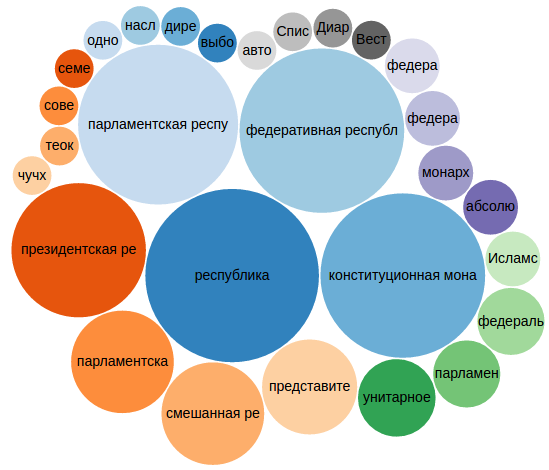
\includegraphics[width=0.94\linewidth]{./chapter/country/Bubble_chart_forms_of_government_countries_according_to_Wikidata.png}
%        \caption{Пузырьковая диаграмма форм правления стран, 2017 год. Основные формы правления стран: республика (20~стран), конституционная монархия (18 стран), федеративная республика (18), парламентская республика (17) и президентская республика (12~стран).} 
%	    \label{fig:bubble_chart_forms_of_government_countries_2017}%
%\end{minipage}%
%%just a break for lines between two columns of listings
%\hfill
%\begin{minipage}[]{.46\linewidth}
%    \centering
%	\includegraphics[width=0.95\linewidth]{./chapter/country/Bubble_chart_forms_of_government_countries_according_to_Wikidata_2020.png}
%    \caption{Пузырьковая диаграмма форм правления стран, 2020 год.
%	\\
%	По данным на 2020 год  основные формы правления стран: республика (в~41~стране), конституционная монархия (32), федеративная республика (19), парламентская республика (22) и президентская республика (14).} 
%	\label{fig:bubble_chart_forms_of_government_countries_2020}%
%\end{minipage}
%\end{fullwidth}%


%\begin{figure}
%		\setlength{\fboxsep}{0pt}%
%		\setlength{\fboxrule}{1pt}%
%		\fcolorbox{gray}{gray}{\includegraphics[width=\linewidth]{./chapter/country/Bubble_chart_forms_of_government_countries_according_to_Wikidata.png}}%
%	\caption
%	[Пузырьковая диаграмма форм правления стран, 2017 год.]
%	{Пузырьковая диаграмма форм правления стран, 2017 год.
%		\\			
%		По данным на 2017 год основные формы правления стран: республика (в 20 странах), конституционная монархия (в 18 странах), федеративная республика (18), парламентская республика (17) и президентская республика (12).}%
%	\label{fig:bubble_chart_forms_of_government_countries_2017}%
%\end{figure}

%\begin{figure}
%		\setlength{\fboxsep}{0pt}%
%		\setlength{\fboxrule}{1pt}%
%		\fcolorbox{gray}{gray}{\includegraphics[width=\linewidth]{./chapter/country/Bubble_chart_forms_of_government_countries_according_to_Wikidata_2020.png}}%
%	\caption
%	[Пузырьковая диаграмма форм правления стран, 2020 год.]
%	{Пузырьковая диаграмма форм правления стран, 2020 год.
%	\\
%	По данным на 2020 год  основные формы правления стран: республика (в 41 стране), конституционная монархия (32), федеративная республика (19), парламентская республика (22) и президентская республика (14).
%}%
%	\label{fig:bubble_chart_forms_of_government_countries_2020}%
%\end{figure}




\newpage
%%%%%%%%%%%%%%%%%%%%%%%%%%%%%%%%%%%%%%%%%%%%%%%%%%%%%%%
\section{Граф соседних стран}
%
\begin{marginfigure}%[7\baselineskip]
	{
		\setlength{\fboxsep}{0pt}%
		\setlength{\fboxrule}{1pt}%
		\fcolorbox{gray}{gray}{\includegraphics[width=\linewidth]{./chapter/country/Neighboring_countries_graph_in_russian_according_to_Wikidata_2017.png}}%
	}
    \caption[Фрагмент графа соседних стран, 2017 год.]{Фрагмент графа соседних стран, в центре Россия, 2017 год}
	\label{fig:neighboring_countries_2017}%
\end{marginfigure}


У стран существует такое свойство, как общая граница. 
В Викиданных это свойство называется 
\href{https://www.wikidata.org/wiki/Property:P47}{shares border with (P47)}. 
Используя его, построим граф соседних стран (запрос~\ref{lst:neighboring_countries}).

\index{График!Graph}
\begin{lstlisting}[ language=SPARQL, 
    caption={\href{https://w.wiki/5Bsy}{Соседние страны}\protect\footnotemark},
    label=lst:neighboring_countries, 
    numbers=none,
]
# Graph of countries which share border
#defaultView:Graph
SELECT DISTINCT ?country ?countryLabel ?border ?sharesBorderWith WHERE
{
    ?country p:P31 [ps:P31 wd:Q6256]. # instance of a country
    OPTIONAL {?country wdt:P47 ?sharesBorderWith}
    SERVICE wikibase:label {bd:serviceParam wikibase:language "ru,en"}
}
\end{lstlisting}
\footnotetext{Получено: 787 соседств на 2017 год и 912 соседств на 2021 год. Ссылка на~SPARQL-запрос: \href{https://w.wiki/5Bsy}{https://w.wiki/5Bsy}.} 

В результате выполнения запроса мы получаем граф с 787 ребрами на 2017 год 
(рис.~\ref{fig:neighboring_countries_2017}) 
и 912 ребрами на 2021 год (рис.~\ref{fig:neighboring_countries_2020}), 
где ребро указывает на общую границу двух стран. 
Граф представляет из~себя несколько связных компонент, 
так как есть островные страны, у которых нет соседей 
(например, \href{https://w.wiki/vC7}{Маврикий} и \href{https://w.wiki/vC8}{Мальдивы}). 
Также стоит упомянуть, что теперь свойство {\textit{shares border with}} 
включает общую не только сухопутную, но и морскую границу. 
Поэтому теперь этот граф будет представлять одну связную компоненту. 

Обратите внимание, что полученный граф (рис.~\ref{fig:neighboring_countries_2017}) 
включает также исторические страны, например СССР. 
Постройте аналогичный граф, но только с современными странами. 
Для этого посмотрите на~запрос~\ref{lst:list_of_country_instance_of_}, где показано, 
как <<выключить>> исторические страны и оставить только действующие. 

\begin{marginfigure}
	{
		\setlength{\fboxsep}{0pt}%
		\setlength{\fboxrule}{1pt}%
		\fcolorbox{gray}{gray}{\includegraphics[width=\linewidth]{./chapter/country/Neighboring_countries_graph_in_russian_according_to_Wikidata_2020.png}}%
	}
    \caption[Фрагмент графа соседних стран, 2020 год.]{Фрагмент графа соседних стран, в центре Россия, 2020 год}
	\label{fig:neighboring_countries_2020}%
\end{marginfigure}



\newpage
\subsection{Карта соседних стран России}
%
\begin{marginfigure}[2\baselineskip]
	{
		\setlength{\fboxsep}{0pt}%
		\setlength{\fboxrule}{1pt}%
		\fcolorbox{gray}{gray}{\includegraphics[width=\linewidth]{./chapter/country/Map_of_neighboring_countries_of_Russia_ru.png}}%
	}
    \caption[Карта соседних стран России, 2021 год.]{Карта соседних стран России, включающая 17~стран, 2021 год}
	\label{fig:neighboring_countries_ru_2020}%
\end{marginfigure}


Построим карту соседних стран России с помощью запроса~\ref{lst:neighboring_countries_ru}.
Строка~6 запроса~\ref{lst:neighboring_countries_ru} 
фильтрует и оставляет в переменной \lstinline|?border_country| только страны.
Это позволило исключить, например, район Грузии (Рача-Лечхуми и Квемо-Сванети) 
и остров Японии (Хоккайдо), указанные в списке пограничных объектов России.

В результате выполнения запроса~\ref{lst:neighboring_countries_ru} мы получили 
карту соседних стран России 
(рис.~\ref{fig:neighboring_countries_ru_2020}), включающую 17 стран, а именно: 
\wdqName{Япония}{17}, \wdqName{Норвегия}{20}, \wdqName{США}{30}, \wdqName{Финляндия}{33}, \wdqName{Швеция}{34}, \wdqName{Польша}{36}, \wdqName{Литва}{37}, \wdqName{Китайская Народная Республика}{148}, \wdqName{Белоруссия}{184}, \wdqName{Эстония}{191}, \wdqName{Латвия}{211}, \wdqName{Украина}{212}, \wdqName{Азербайджан}{227}, \wdqName{Грузия}{230}, \wdqName{Казахстан}{232}, \wdqName{КНДР}{423} и \wdqName{Монголия}{711}.


\index{График!Map}
\index{SPARQL!Свойство!geoshape}
\begin{lstlisting}[ language=SPARQL, 
    caption={\href{https://w.wiki/tg3}{Соседние страны России}\protect\footnotemark},
    label=lst:neighboring_countries_ru, 
]
# Map of neighboring countries of Russia
#defaultView:Map
SELECT ?border_country ?border_countryLabel ?coords ?layer WHERE 
{                                         # border\_country
	?border_country p:P47 [ps:P47 wd:Q159]. #   has border with Russia
	?border_country p:P31 [ps:P31 wd:Q6256].#   is a country
	OPTIONAL {?border_country wdt:P3896 ?coords.} # geoshape
	BIND (?coords AS ?layer)
	SERVICE wikibase:label { bd:serviceParam wikibase:language "ru". }
}
\end{lstlisting}
\footnotetext{Получено: 17 стран на 2021 год. Ссылка на SPARQL-запрос: \href{https://w.wiki/tg3}{https://w.wiki/tg3}.}


%%%%%%%%%%%%%%%%%%%%%%%%%%%%%%%%%%%%%%%%%%%%%%%%%%%%%%%
\section{Упражнения}

\begin{enumerate}[noitemsep,topsep=0pt]
	\item Постройте список флагов и девизов стран. Девизы есть не у всех стран.
	\item Отметьте на карте столицы современных стран.
	\item В каждой части света вычислите первые пять стран с наибольшей плотностью населения.
	\item Постройте столбчатую диаграмму, демонстрирующую распределение количества стран по формам правления.
	\item Выведите список стран, упорядоченных по числу соседей. 
        У каких стран больше всего и~меньше всего соседей? Какое среднее число соседей? 
        Есть ли корреляция между этим показателем и каким-либо другим параметром стран?
\end{enumerate}

\chapter[В каких населённых пунктах России больше рождаётся учёных, в сельских или городских?]{В каких населённых пунктах России больше рождаётся учёных,\\в сельских или городских?}
\label{ch:human-settlement}

В главе исследуется объект Викиданных <<\wdqName{населённый пункт}{486972}>> и его свойства. 
В~каждом из разделов представлены задачи, решённые с помощью SPARQL-запросов. 
%
%%%%%%%%%%%%%%%% Упражнение 1 %%%%%%%%%%%%%%%% 
\marginnote{%
    \MarginQuestion
    Подсчитайте, сколько человек на~1~км\textsuperscript{2} живёт в~\ruwiki{4dNv}{Барабинске} 
и в~\ruwiki{4dNt}{Алейске}? В~каком из этих \emph{населённых пунктов} плотность населения выше?

См. ответ~\ref{answer:human_settlements_density} на с.~\pageref{answer:human_settlements_density}.%
}

Был получен список населённых пунктов, 
построены пузырьковые диаграммы с количеством населения в <<населённых пунктах>> по странам. 
Построена диаграмма, показывающая долю населения, 
проживающего в населённых пунктах относительно всего населения страны. 
Диаграмма показала, что высокий процент населения, проживающего в~населённых пунктах, 
приходится на сельскохозяйственные страны, в то время как в более индустриальных странах 
меньшая доля населения проживает в населённых пунктах. 
%
%%%%%%%%%%%%%%%% Упражнение 2 %%%%%%%%%%%%%%%%
\marginnote{%
\MarginQuestion Герб какого отечественного или зарубежного населённого пункта изображён на рисунке?

    \includegraphics[width=2cm]{./chapter/human_settlement/Aznakeevskii_rayon_gerb.png}

    См. ответ~\protect\ref{answer:flag_human_settlements} на с.~\protect\pageref{answer:flag_human_settlements}.
%  \label{fig:flag_question_human_settlements1}%
}

На 2017 год Википедия описывала примерно половину населённых пунктов (75 тыс.), 
Викиданные содержали менее 3\,\% таких поселений (4 тыс.) относительно данных переписи за 2010 год (155,5 тыс.). 
На 2021 год Викиданные содержат менее 12\,\% таких поселений (17 тыс.) 
относительно данных той же переписи за 2010 год. 

Для сравнения сельских и городских поселений 
построены диаграммы количества учёных, сгруппированных по родам деятельности 
и разделённых по месту рождения~--- сельское или городское.

Для поиска более полных ответов на поставленные выше задачи  
были найдены более общие классы для объекта <<\wdqName{населённый пункт}{486972}>> 
с помощью свойства <<\wdProperty{31}{частный случай понятия}>>. 
Трудность исследования вызвана отсутствием чёткой типологии населённых пунктов 
(например, от численности населения) в законодательстве России и в~Викиданных.



%%%%%%%
\section{Список <<населённых пунктов>>}
%%%%%%%%%%%%%%%% Упражнение 2 %%%%%%%%%%%%%%%%
\begin{marginfigure}[0.0cm]
{\includegraphics[width=5cm]{./chapter/human_settlement/Coat_of_Arms_of_Asbest_(Sverdlovsk_oblast).png}}
  \caption[Герб второго неизвестного населённого пункта.]{Это герб населённого пункта России или другой страны?\newline%
См. ответ~\protect\ref{answer:flag_human_settlements} на с.~\protect\pageref{answer:flag_human_settlements}.}
  \label{fig:flag_question_human_settlements2}%
\end{marginfigure}

Построим список всех населённых пунктов с помощью запроса~\ref{lst:human-settlement1}.

\begin{lstlisting}[ language=SPARQL, 
                    caption={\href{https://w.wiki/4d7x}{Список всех населённых пунктов}\protect\footnotemark},
                    label=lst:human-settlement1,
                    texcl 
                    ]
# List of all human settlements
SELECT ?hum ?humLabel WHERE{
  ?hum wdt:P31 wd:Q486972. # instance of human settlement
  SERVICE wikibase:label{bd:serviceParam wikibase:language "ru,en"}
}
\end{lstlisting}%
\footnotetext{Получено \num{411393} пунктов в 2017 году. SPARQL-запрос: \href{https://w.wiki/4d7x}{https://w.wiki/4d7x}}

В 2021 году оказалось невозможным получить список населённых пунктов 
из-за большого числа объектов и поэтому слишком долгой работы запроса~\ref{lst:human-settlement1}. 
Для подсчёта числа всех населённых пунктов обратимся к функции \lstinline|COUNT()| 
в запросе~\ref{lst:human-settlement-count-classes}.

\index{SPARQL!COUNT!Количество всех населённых пунктов}
\begin{lstlisting}[ language=SPARQL, 
                    caption={\href{https://w.wiki/4d7s}{Количество всех населённых пунктов}\protect\footnotemark},
                    label=lst:human-settlement-count-classes,
                    texcl 
                    ]
# Number of human settlements
SELECT (COUNT(?hum) AS ?count) WHERE {
  ?hum wdt:P31 wd:Q486972. # instance of human settlement  
}
\end{lstlisting}%
\footnotetext{Получено: \num{563126} населённых пунктов в 2021 году. SPARQL-запрос: \href{https://w.wiki/4d7s}{https://w.wiki/4d7s}.}

Среди отечественных населённых пунктов на Викиданных, 
которым соответствуют статьи Русской Википедии, 
почти пустыми являются, например, 
бывшая деревня \wdqName{Борисово}{4093951} (3 свойства) 
и \wdqName{Бригадирское лесничество}{21668554} (4 свойства).

По данным сервиса ProWD, 
среди отечественных населённых пунктов 
больше всего свойств (36) у \wdqName{Ялты}{128499}. 
Лидером по всему миру является \wdqName{Токио}{1490} (73 свойства)\autocite{humansettlements_ProWD}.



%%%%%%%
\section{Список стран по суммарному количеству населения}

%\marginnote{%
%См. ответ~\ref{answer:flag_human_settlements} на с.~\pageref{answer:flag_human_settlements}.
%}
С помощью запроса~\ref{lst:human-settlement3} 
построим упорядоченный список стран по суммарному количеству населения, проживающего в <<населённых пунктах>>.


%\begin{minipage}{\linewidth}
%\marginnote[0cm]{Получена \num{161} страна в 2017 году и \num{213} стран в 2021 году. SPARQL-запрос: \href{https://w.wiki/4d9M}{https://w.wiki/4d9M}}
\index{SPARQL!SUM!Список стран по суммарному количеству населения, проживающего в <<населённых пунктах>>}
\index{SPARQL!GROUP BY!Список стран по суммарному количеству населения, проживающего в <<населённых пунктах>>}
\lstset{numbers=left, firstnumber=1, frame=single}
\begin{lstlisting}[ language=SPARQL, 
    caption={\href{https://w.wiki/4d9M}{Список стран по суммарному количеству населения, проживающего в <<населённых пунктах>>}\protect\footnotemark},
    label=lst:human-settlement3,
    texcl 
                  ]
# List of countries by population in settlements
SELECT ?country ?countryLabel (SUM(?population) as ?sumPopulation)
WHERE {
  ?hum wdt:P31 wd:Q486972;      # instance of human settlement
       wdt:P17 ?country;        # in the ?country
       wdt:P1082 ?population.   # has ?population
  SERVICE wikibase:label{bd:serviceParam wikibase:language "ru,en"}
}
GROUP BY ?country ?countryLabel 
ORDER BY DESC (?sumPopulation)
\end{lstlisting}%
\footnotetext{Получено: \num{161} страна в 2017 году и \num{213} стран в 2021 году. Ссылка на SPARQL-запрос: \href{https://w.wiki/4d9M}{https://w.wiki/4d9M}.}
%\end{minipage}


Для подсчёта количества населения по странам 
используем команду \lstinline|SUM()| во второй строке запроса~\ref{lst:human-settlement3}. 
Для группировки населённых пунктов по странам 
используем команду \lstinline|GROUP BY| на девятой строке того же запроса.

Пузырьковая диаграмма на рис.~\ref{fig:human-settlement-1} и~\ref{fig:human-settlement-2} 
показывает соотношение стран по количеству населения в <<населённых пунктах>> 
в~2017 и~2021~годах соответственно. 
Размер пузырька соответствует количеству населения, проживающего в <<населённых пунктах>> одной страны. 
Ссылка на SPARQL-запрос: \href{https://w.wiki/4dAv}{https://w.wiki/4dAv}.

%\begin{fullwidth}
%\noindent\begin{minipage}[]{.46\linewidth}
%    \centering
\begin{marginfigure}[0.0cm]
	    \includegraphics[width=0.94\linewidth]{./chapter/human_settlement/AnnaBubbleHumanSettlement.jpg}
        \caption[Сколько населения проживает в населённых пунктах, 2017.]{Пузырьковая диаграмма с суммарным количеством населения, проживающего в <<населённых пунктах>> на 2017 год} 
        %Размер пузырька соответствует количеству населения, проживающего в <<населённых пунктах>> одной страны. Ссылка на SPARQL-запрос: \href{https://w.wiki/4dAv}{https://w.wiki/4dAv}}
	    \label{fig:human-settlement-1}
\end{marginfigure}
%\end{minipage}%
%just a break for lines between two columns of listings
%\hfill
%\begin{minipage}[]{.46\linewidth}
%    \centering
\begin{marginfigure}[0.0cm]
	\includegraphics[width=0.95\linewidth]{./chapter/human_settlement/LeonidBubbleHumanSettlement.jpg}
    \caption[Сколько населения проживает в населённых пунктах, 2021.]{Пузырьковая диаграмма с суммарным количеством населения, проживающего в <<населённых пунктах>> на 2021 год} 
    %Размер пузырька соответствует количеству населения, проживающего в <<населённых пунктах>> одной страны. Ссылка на SPARQL-запрос: \href{https://w.wiki/4dAv}{https://w.wiki/4dAv}}
	\label{fig:human-settlement-2}
\end{marginfigure}
%\end{minipage}
%\end{fullwidth}%



%\begin{figure}
%\centering
%	\includegraphics[width=0.9\linewidth]{./chapter/human_settlement/AnnaBubbleHumanSettlement.jpg}
%	\label{fig:human-settlement-1}
%    \caption[Пузырьковая диаграмма с суммарным количеством населения в населённых пунктах, 2017 год.]{Пузырьковая диаграмма с суммарным количеством населения, проживающего в <<населённых пунктах>> на 2017 год. Размер пузырька соответствует количеству населения, проживающего в <<населённых пунктах>> одной страны. Ссылка на SPARQL-запрос: \href{https://w.wiki/4dAv}{https://w.wiki/4dAv}}
%\end{figure}

%\begin{figure}
%\centering
%	\includegraphics[width=0.9\linewidth]{./chapter/human_settlement/LeonidBubbleHumanSettlement.jpg}
%	\label{fig:human-settlement-2}
%	\caption[Пузырьковая диаграмма с суммарным количеством населения в населённых пунктах, 2021 год.]{Пузырьковая диаграмма с суммарным количеством населения, проживающего в <<населённых пунктах>> на 2021 год. Размер пузырька соответствует количеству населения, проживающего в <<населённых пунктах>> одной страны. Ссылка на SPARQL-запрос: \href{https://w.wiki/4dAv}{https://w.wiki/4dAv}}
%\end{figure}

В 2017 году больше всего населения проживало в <<населённых пунктах>> 
\wdqName{Бразилии}{155} (\num{12} млн), 
\wdqName{Пакистана}{843} (\num{10} млн), 
\wdqName{Мексики}{96} (\num{8} млн), 
\wdqName{Йемена}{805} (\num{8} млн), 
\wdqName{Индии}{668} и 
\wdqName{Бангладеша}{902} (по \num{7} млн). 

На рис.~\ref{fig:human-settlement-2} можно увидеть список стран на 2021 год: 
\wdqName{Индия}{668} (\num{30} млн), 
\wdqName{Китай}{148} (\num{28} млн), 
\wdqName{Мексика}{96} (\num{17} млн), 
\wdqName{Индонезия}{252} (\num{13} млн), 
\wdqName{Канада}{16} (\num{9} млн) и 
\wdqName{Саудовская Аравия}{851} (\num{9} млн). 

Итак, результаты запроса~\ref{lst:human-settlement3} в 2017 и 2021 существенно разнятся. 
По этим результатам получается, что за четыре года 
в населённых пунктах Индии стало больше на 23 млн человек. 


%%%%%
\subsection{Полнота Викиданных}

Населённый пункт~--- это общее название мест с постоянными жителями\autocite{Humansettlements_Dictionary}. 
По версии редакторов Викиданных в понятие насёленный пункт входят города, сёла, деревни 
и другие\marginnote[4pt]{Полный список можно увидеть в разделе <<Cписок классов, сопутствующих ``населённому пункту'' в свойстве ``экземпляр''>> на с.~\pageref{human-settlement:tag1}.}.
Точной информации о количестве населённых пунктов в мире мы не нашли. 
Поэтому проверим полноту тех населённых пунктов, которые есть в Викиданных 
и которые использовались для решения задачи. 
В задачах выше мы использовали свойста \wdProperty{1082}{численность населения} и 
\wdProperty{17}{государство} (привязка к стране). 
Исходя из этого проверку полноты разделим на подзадачи: 
\begin{enumerate} 
  \item Проверка заполненности свойства <<численность населения>>.
  \item Проверка принадлежности к государству.
\end{enumerate}


%%%%%
\subsection{Проверка заполненности свойства <<численность населения>> }

Для такой проверки напишем \href{https://w.wiki/4FUz}{SPARQL-запрос}\sidenote{
%
В 2017 году запрос выдал \num{372997} населённых пунктов 
с незаполненным свойством <<численность населения>>. 
Тот же запрос в 2021 году выдал \num{507078} таких населённых пунктов. 
Ссылка на SPARQL-запрос: \href{https://w.wiki/4FUz}{https://w.wiki/4FUz}% 
}, 
который выведет населённые пункты 
с незаполненным свойством \href{http://www.wikidata.org/entity/P1082}{численность населения}. 
Произведя расчёты получаем, что только у 9,3\% населенных пунктов мира 
указано свойство <<численность населения>> на 2017 год. 
В 2021 получаем 11,2\% населенных пунктов мира с заполненным свойство <<численность населения>>. 
Итак, одновременно с ростом числа населённых пунктов в Викиданных 
растёт доля пунктов с заполненным свойством <<численность населения>>.


%%%%%
\subsection{Проверка принадлежности к государству}

А теперь посмотрим населённые пункты, 
у которых не указана принадлежность к какой-либо стране 
с помощью \href{https://w.wiki/4FV8}{SPARQL-запроса}\footnote{%
%
В 2017 году нашлось \num{8427} объектов, у которых не указана принадлежность к какой-либо стране. 
В 2021 году таких объектов уже больше~--- \num{27824}. 

SPARQL-запрос: \href{https://w.wiki/4FV8}{https://w.wiki/4FV8}.%
}. 

Результаты запроса показывают, что число пунктов без привязки к стране растёт с годами. 
Поэтому вычисления, связанные с населёнными пунктами и странами, 
по определению будут не полными даже относительно тех пунктов, которые уже есть в Викиданных. 


%%%%%
\section{Доля населения страны, проживающего в <<населённых пунктах>>}

Построим список стран, 
упорядоченный по доли населения (в~процентах), проживающей в \href{http://www.wikidata.org/entity/Q486972}{населённых пунктах}, относительно числа всех жителей страны (листинг~\ref{lst:human-settlement6}).

\index{SPARQL!SUM!Соотношение количества людей, проживающих в населённых пунктах, к количеству всех людей в стране}
\begin{lstlisting}[ language=SPARQL, 
                    caption={\href{https://w.wiki/4dE3}{Соотношение количества людей, проживающих в населённых пунктах, к количеству всех людей в стране}\protect\footnotemark},
                    label=lst:human-settlement6,
                    texcl 
                    ]
# An ordered list of the ratio of the number of people living in 
# "human\_settlement" to the number of inhabitants in the country.
SELECT ?country ?countryLabel ?proportionPopulation WHERE {
 SELECT ?country ?countryLabel (SUM(?population / ?pop) 
        as ?proportionPopulation) WHERE {
  ?hum wdt:P31 wd:Q486972;    # instances of human settlement  
       wdt:P17 ?country;         # has ?country 
       wdt:P1082 ?population.    # has ?population
  ?country wdt:P1082 ?pop.    # population in the country
  SERVICE wikibase:label{bd:serviceParam wikibase:language "ru,en"}
 }
 GROUP BY ?country ?countryLabel
}
ORDER BY ?proportionPopulation
\end{lstlisting}%
%
%%%%%%%%%%%%%%%% Упражнение 2 %%%%%%%%%%%%%%%%
\begin{marginfigure}[-23\baselineskip]
{\includegraphics[width=5cm]{./chapter/human_settlement/Loučovice_CoA.jpg}}
  \caption[Герб третьего неизвестного населённого пункта.]{Герб населённого пункта какой страны изображён?\newline 
            См. ответ~\ref{answer:flag_human_settlements} на с.~\pageref{answer:flag_human_settlements}.}%
  \label{fig:flag_question_human_settlements3}%
\end{marginfigure}
%\marginnote{%
%См. ответ~\ref{answer:flag_human_settlements} на с.~\pageref{answer:flag_human_settlements}.%
%}
\footnotetext{Получено: \num{158} результатов в 2017 году и \num{206} результатов в 2021 году. Ссылка на SPARQL-запрос: \href{https://w.wiki/4dE3}{https://w.wiki/4dE3}}

Столбчатая диаграмма на рис.~\ref{fig:human-settlement-3} позволяет увидеть для каждой страны 
отношение количества людей, 
проживающих в~\href{http://www.wikidata.org/entity/Q486972}{населённых пунктах}, 
к~числу жителей в~стране на 2017 год.


По рис.~\ref{fig:human-settlement-3} видно, 
что наиболее высокий процент в 2017 году приходился на следующие страны: 
Кирибати (78\%), Ниуэ (70\%), Греция (53\%), Тувалу (48\%), Коморы (43\%), Маврикий (42\%). 
В 2022 году картина изменилась: Нигерия (93\%), Папуа~--- Новая Гвинея (71\%), 
Израиль (50\%), Греция (47\%), Азербайджан (47\%), Казахстан (37\%). 



На 2017 год в странах большой восьмёрки доля жителей 
в \href{http://www.wikidata.org/entity/Q486972}{населённых пунктах} составила: 
\href{http://www.wikidata.org/entity/Q159}{Россия} (\num{2.98}\%), 
\href{http://www.wikidata.org/entity/Q30}{США} (\num{1.76}\%), 
\href{http://www.wikidata.org/entity/Q17}{Япония} (\num{0.80}\%), 
\href{http://www.wikidata.org/entity/Q16}{Канада} (\num{0.26}\%), 
\href{http://www.wikidata.org/entity/Q142}{Франция} (\num{0.20}\%), 
\href{http://www.wikidata.org/entity/Q183}{Германия} (\num{0.24}\%), 
\href{http://www.wikidata.org/entity/Q145}{Великобритания} (\num{0.18}\%), 
\href{http://www.wikidata.org/entity/Q38}{Италия} (\num{0.07}\%). 
В 2022 году значения доли населения снизились (рис.~\ref{fig:human-settlement-4}): 
\href{http://www.wikidata.org/entity/Q159}{Россия} (0.045\%), 
\href{http://www.wikidata.org/entity/Q30}{США} (\num{0.014}\%), 
\href{http://www.wikidata.org/entity/Q17}{Япония} (\num{0.008}\%), 
\href{http://www.wikidata.org/entity/Q16}{Канада} (\num{0.23}\%), 
\href{http://www.wikidata.org/entity/Q142}{Франция} (\num{0.005}\%), 
\href{http://www.wikidata.org/entity/Q183}{Германия} (\num{0.005}\%), 
\href{http://www.wikidata.org/entity/Q145}{Великобритания} (\num{0.014}\%), 
\href{http://www.wikidata.org/entity/Q38}{Италия} (\num{0.0005}\%). 
Отметим, что это страны промышленно развитые.

\begin{figure*}
    \includegraphics[width=1\linewidth]{./chapter/human_settlement/AnnaShareHumanSettlement.png}
	\label{fig:human-settlement-3}
	\caption[Диаграмма доли населения страны, проживающего в населённых пунктах, 2017 год.]{Диаграмма доли населения страны, проживающего в <<населённых пунктах>> на 2017 год. Ссылка на SPARQL-запрос: \href{https://w.wiki/4dE3}{https://w.wiki/4dE3}}%
\end{figure*} 


\begin{figure*}
% see https://commons.wikimedia.org/wiki/File:Proportion_of_the_country%27s_population_living_in_human_settlements_for_2022.png    
    \includegraphics[width=1\linewidth]{./chapter/human_settlement/ShareHumanSettlement_2022.png}
	\label{fig:human-settlement-4}
	\caption[Диаграмма доли населения страны, проживающего в населённых пунктах, 2021 год.]{Диаграмма доли населения страны, проживающего в <<населённых пунктах>> на 2022 год. Были выбраны страны с населением более 5 млн чел. SPARQL-запрос: \href{https://w.wiki/5Ajn}{https://w.wiki/5Ajn}}%
\end{figure*}%

Поставим вопрос читателю относительно запроса \href{https://w.wiki/5Ajn}{https://w.wiki/5Ajn}, 
с помощью которого построен рис.~\ref{fig:human-settlement-4}. 
А именно к 13 строчке: \lstinline|HAVING (?proportionPopulation > 0.1 && ?proportionPopulation < 1)|. 
Как вы думаете, в каких случаях доля населения, живущего в~населённых пунктах может превышать 100 \%?


%%%%%%%%%%%%%%%% Упражнение 2 %%%%%%%%%%%%%%%%
\begin{marginfigure}[0.0cm]
{\includegraphics[width=4cm]{./chapter/human_settlement/POL_Otynia_COA.png}}
  \caption[Герб четвёртого неизвестного населённого пункта.]{Герб населённого пункта какой страны изображён?\newline
См. ответ~\ref{answer:flag_human_settlements} на с.~\pageref{answer:flag_human_settlements}.}%
  \label{fig:flag_question_human_settlements4}%
\end{marginfigure}
%\marginnote{%
%См. ответ~\ref{answer:flag_human_settlements} на с.~\pageref{answer:flag_human_settlements}.%
%}

Полученные диаграммы подтверждают следующую гипотезу: 
высокий процент населения страны, проживающего в~<<населённых пунктах>>, 
указывает на более аграрную страну. 
Из диаграмм~\ref{fig:human-settlement-3} и~\ref{fig:human-settlement-4} видно, 
что наиболее высокий процент населения, проживающего в населённых пунктах, 
приходится на страны, в которых, по-видимому, менее развита промышленность. 
А индустриальные страны (например, страны большой восьмёрки) имеют очень низкий процент населения страны, 
проживающего в~населённых пунктах.




%%%%%
\section[Cписок классов, сопутствующих <<населённому пункту>> в~свойстве <<экземпляр>>]{Cписок классов, сопутствующих <<населённому пункту>>\\в~свойстве <<экземпляр>>}
\label{human-settlement:tag1}

Будем называть <<классом>> такие объекты Викиданных, 
которые связаны с каким-либо объектом Викиданных посредством свойства \wdProperty{31}{экземпляр}. 
Цель этого раздела~--- найти объекты $X$, 
для которых объект \wdqName{населённый пункт}{486972} является \emph{классом}, 
и получить другие классы объекта $X$, кроме <<населённого пункта>>. 
Эти <<другие>> классы будет называть сопутствующими <<населённому пункту>>. 
С помощью запроса~\ref{lst:human-settlement7} 
найдём объекты, сопутствующие <<населённому пункту>>. 


%%%%%%%%%%%%%%%% Упражнение 2 %%%%%%%%%%%%%%%%
\begin{marginfigure}[0cm]
{\includegraphics[width=4cm]{./chapter/human_settlement/Coat_of_Arms_of_Azov.png}}
  \caption[Герб пятого неизвестного населённого пункта.]{Герб населённого пункта какой страны изображён?\\
См. ответ~\ref{answer:flag_human_settlements} на с.~\pageref{answer:flag_human_settlements}.}%
  \label{fig:flag_question_human_settlements5}%
\end{marginfigure}
%\marginnote{%
%См. ответ~\ref{answer:flag_human_settlements} на с.~\pageref{answer:flag_human_settlements}.%
%}

%\marginnote[1cm]{Получено 610 результатов в 2017 году и \num{1245} результатов в 2021 году. SPARQL-запрос: \href{https://w.wiki/4dEW}{https://w.wiki/4dEW}}
\begin{lstlisting}[ language=SPARQL, 
    caption={\href{https://w.wiki/4dEW}{Cписок объектов, сопутствующих <<населённому пункту>>}\protect\footnotemark},
    label=lst:human-settlement7,
    texcl 
                  ]
# List of classes accompanying the human\_settlement (instance of)
SELECT ?inst (COUNT(?hum) as ?sumHum) 
WHERE{          
  ?hum wdt:P31 wd:Q486972; # instance of human settlement
       wdt:P31 ?inst.      # other objects in instance
  SERVICE wikibase:label{bd:serviceParam wikibase:language "ru,en"}
}  
GROUP BY ?inst
\end{lstlisting}%
\footnotetext{Получено: 610 результатов в 2017 году и \num{1245} результатов в 2021 году. SPARQL-запрос: \href{https://w.wiki/4dEW}{https://w.wiki/4dEW}}

Для ускорения выполнения запроса~\ref{lst:human-settlement7} выполним два шага.
 
Во-первых, выключим из рассмотрения поселения, 
имеющие в~списке экземпляров только <<населённый пункт>>, 
поскольку других сопутствующих классов нет. 
Для этого добавим в скрипт~\ref{lst:human-settlement8} строку~\num{9} с фильтром, 
требующим, чтобы у объекта \lstinline|?hum| 
кроме \wdProperty{31}{экземпляра} \wdqName{населённый пункт}{486972} был ещё какой-либо класс.

Во-вторых, в строке \num{8} запроса~\ref{lst:human-settlement8} 
уберём такие объекты переменной \lstinline|?inst|, 
которые имеют свойство \wdqName{государство}{17}. 
Это позволит отсечь сотни типов населённых пунктов специфичных для отдельных стран, 
например, <<административно-территориальная единица России>>.

Эти преобразования позволили выполнить запрос~\ref{lst:human-settlement8} 
по всем странам мира за приемлемое время в 13 мс.

\lstset{numbers=left, firstnumber=1, frame=single}
\begin{lstlisting}[ language=SPARQL, 
    caption={\href{https://w.wiki/4ePf}{Cписок классов, сопутствующих <<населённому пункту>> в свойстве <<экземпляр>> без специализированных классов разных стран}\protect\footnotemark},
    label=lst:human-settlement8,
    texcl 
                  ]
# List of objects with the class of human settlement, without 
# country and single human settlement
SELECT ?inst ?instLabel (COUNT(?hum) as ?sumHum) 
WHERE{ 
  ?hum wdt:P31 wd:Q486972;  # instance of human settlement
       wdt:P31 ?inst.       # other objects in instance
  
  MINUS {?inst wdt:P17 []}. # without country
  FILTER(?inst != wd:Q486972 ). # without human settlement
  SERVICE wikibase:label{bd:serviceParam wikibase:language "ru,en"}
}  
GROUP BY ?inst ?instLabel
ORDER BY DESC (?sumHum)
\end{lstlisting}%
\footnotetext{Получено 355 записей в 2017 году и 707 записей в 2021 году. Ссылка на SPARQL-запрос: \href{https://w.wiki/4ePf}{https://w.wiki/4ePf}}

В таблице~\ref{tab:human-settlement-classes} представлены классы, 
сопутствующие <<населённому пункту>> в свойстве <<экземпляр>>, 
и сравнение количества этих классов за 2017 и 2021 годы.

\begin{table}[h]
\centering
\begin{tabular}{|l|l|l|l|l|}
\hline
\textnumero & Название класса населённого пункта & 2017 & 2021 & $\Delta$ \\ \hline
1 & \wdqName{Cело}{532}                  & \num{2844}       & \num{4853} & +\num{2009}	\\
2 & \wdqName{Муниципалитеты}{15284}      & \num{1181}       & \num{3376} & +\num{2195}	\\
3 & \wdqName{Деревни}{5084}              & \num{662}        & \num{1761} & +\num{1099}	\\ 
4 & \wdqName{Археологические памятники}{839954}	& \num{425} & \num{887}	& +\num{462}	\\ 
5 & \wdqName{Местные поселения}{3257686} & \num{425}        & \num{158}	& -\num{257}	\\ 
6 & \wdqName{Разрушенные города}{14616455} & \num{423}      & \num{388}	& -\num{40}	\\
7 & \wdqName{Города}{515}                 & \num{322}       & \num{545}	& +\num{223}	\\
8 & \wdqName{Малые города}{3957}		  & \num{277}       & \num{446}	& +\num{169}	\\ 
9 & \wdqName{Заброшенные деревни}{350895} & \num{254}       & \num{474}	& +\num{220}	\\ 
10 & \wdqName{Внутренние районы}{2983893} & \num{207}       & \num{503}	& +\num{296}	\\ \hline
\end{tabular}
    \caption[Сопутствующие населённому пункту классы, 2017 и 2021 годы.]{Количество классов, сопутствующих <<населённому пункту>>, в~2017 и 2021 годы, их разница ($\Delta$). 
    Получены данные по всему миру. В таблице представлены первые строки ответа на запрос~\protect\ref{lst:human-settlement9}.}
\label{tab:human-settlement-classes}
\end{table}   



Запрос~\ref{lst:human-settlement8} показал, что на 2021 год на первых местах 
среди сопутствующих <<населённому пункту>> классов 
были доисторические поселения трёх типов: поселения 
\wdqName{<<латенского периода>>}{106505016}, 
\wdqName{<<бронзового века>>}{106491277} 
и поселения \wdqName{<<доисторического времени, где есть письменность>>}{106505070}. 

Попробуем сформулировать запрос так, чтобы отсечь всё множество доисторических поселений.  
Что есть общего у этих трёх объектов на Викиданных? 
Они являются экземплярами объектов, которые, в свою очередь, 
являются экземплярами объектов \wdqName{<<археологической культуры>>}{465299}, 
\wdqName{<<исторического периода>>}{11514315}, 
\wdqName{<<археологического века>>}{15401699}, 
\wdqName{<<всемирной истории>>}{200325} 
и \wdqName{<<геологического периода>>}{392928}. 
Применим такой фильтр в запросе~\ref{lst:human-settlement9} в строках 10--12, 
чтобы отсечь именно эти типы объектов.

\begin{fullwidth}
\index{SPARQL!COUNT!Cписок классов, сопутствующих <<населённому пункту>> в свойстве <<экземпляр>>, без исторических объектов}
\index{SPARQL!FILTER!Cписок классов, сопутствующих <<населённому пункту>> в свойстве <<экземпляр>>, без исторических объектов}
\index{SPARQL!MINUS!Cписок классов, сопутствующих <<населённому пункту>> в свойстве <<экземпляр>>, без исторических объектов}
\lstset{numbers=left, firstnumber=1, frame=single}
\begin{lstlisting}[ language=SPARQL, 
                    caption={\href{https://w.wiki/5AdW}{Cписок классов, сопутствующих <<населённому пункту>> в свойстве <<экземпляр>>, без исторических объектов}\protect\footnotemark},
                    label=lst:human-settlement9,
                    texcl 
                    ]
# List of classes accompanying the human\_settlement in the property 'instance of' without historical objects 
SELECT ?inst ?instLabel (COUNT(?hum) as ?sumHum)
WHERE{
  ?hum wdt:P31 wd:Q486972;    # instance of human settlement
       wdt:P31 ?inst.         # other objects in instance of human settlement
  ?inst wdt:P31 [wdt:P31 ?typ]. # instance of instance
  MINUS {?inst wdt:P17 []}.   # without country
  FILTER(?inst != wd:Q486972 && ?typ != wd:Q465299 && ?typ != wd:Q11514315 && ?typ != wd:Q15401699 
         && ?typ != wd:Q200325 && ?typ != wd:Q392928 ). # without human settlement and prehistoric settlements
  SERVICE wikibase:label{bd:serviceParam wikibase:language "ru,en"}
}
GROUP BY ?inst ?instLabel
ORDER BY DESC (?sumHum)
\end{lstlisting}%
\footnotetext{Получено 89 результатов. Ссылка на SPARQL-запрос: \href{https://w.wiki/5AdW}{https://w.wiki/5AdW}}
\end{fullwidth}

В итоге, 707 классов запроса~\ref{lst:human-settlement8} 
мы сократили в~запросе~\ref{lst:human-settlement9} 
до 89 различных классов, сопутствующих <<населённому пункту>> в свойстве <<экземпляр>>. 
В таблице~\ref{tab:human-settlement-classes} представлены первые 10 наиболее частотных классов из 89. 


\newpage

%%%%%
\section{Отечественные учёные на селе и в городе}

Подсчитаем и сравним число отечественных учёных, родившихся в сельских и городских типах населённых пунктов. 
Решим эту задачу в пять шагов:
\begin{enumerate}
  \item Выявим список сельских и список городских типов поселений именно в России.
  \item Определим основные научные направления, представленные в~Викиданных.
  \item Выявим способ определения отечественных учёных.
  \item Сделаем такую диаграмму, на которой разным цветом будут указаны разные научные направления (математики, физики, химики и так далее) для учёных, родившихся в \emph{сельских поселениях}.
  \item Сделаем аналогичную диаграмму, но уже по \emph{городским поселениям} и сравним результаты.
\end{enumerate}


%%%%%
\subsection{Список сельских и список городских типов поселений в~России}%
\label{sec:list-village-city-types-in-Russia}

С помощью запроса~\ref{lst:human-settlement-noname-count} 
Выведем список типов поселений и их количество для объектов, 
имеющих свойство \wdProperty{1082}{<<численность населения>>} 
и принадлежащих \wdqName{России}{159}. 

\marginnote[64pt]{%
%
Задача. Используя команду \lstinline|FILTER~NOT~EXISTS|, 
измените запрос~\ref{lst:human-settlement-noname-count} так, чтобы получить число классов 
с пустым полем <<численность населения>>. 

{\noindent}См. пример использования этой команды в запросе~\ref{lst:anime_no_pub_date} 
на с.~\pageref{lst:anime_no_pub_date}.%
%
}
\index{SPARQL!COUNT!Список классов поселений и их количество для объектов в России, имеющих свойство <<численность населения>>}
\begin{lstlisting}[ language=SPARQL, 
                    caption={\href{https://w.wiki/4zPi}{Список классов поселений и их количество для объектов, имеющих свойство <<численность населения>> в России}\protect\footnotemark},
                    label=lst:human-settlement-noname-count,
                    texcl 
                    ]
# List of instances of settlement with population in Russia
SELECT ?class ?classLabel (COUNT(?class) AS ?count) WHERE {
  SELECT ?class ?classLabel WHERE {
    [] wdt:P31 ?class; # noname instance of class
         wdt:P17 wd:Q159;  # in Russia
         wdt:P1082 [].     # has population
    FILTER(?class != wd:Q486972).# skip settlement itself
    SERVICE wikibase:label{bd:serviceParam wikibase:language "ru"}
  }
}
GROUP BY ?class ?classLabel
ORDER BY DESC (?count)
\end{lstlisting}%
\footnotetext{Получили 229 разных классов поселений в 2022 году. Ссылка на SPARQL-запрос: \href{https://w.wiki/4zPi}{https://w.wiki/4zPi}}

Основные классы поселений, полученные с помощью запроса~\ref{lst:human-settlement-noname-count}, 
представлены в таблице~\ref{tab:human-settlement1}. 

Обратите внимание на безымянные переменные (\lstinline|[]|) 
в строках 4~и~6 запроса~\ref{lst:human-settlement-noname-count}. 
Эта безымянность связана с тем, что 
важен факт указания численности населения, но~не~количество людей в них (строка~6),  
нам не нужны названия сёл и деревень (строка~4).  

Наличие строки шесть в~запросе~\ref{lst:human-settlement-noname-count} 
(\lstinline|wdt:P1082 []|) 
существенно уменьшает числа в таблице~\ref{tab:human-settlement1} 
в~столбце <<Количество>>. 
Это связано с тем, что у многих населённых пунктов 
не~заполнено поле <<численность населения>>. 



\begin{table}[h]
\centering
\begin{tabular}{|r|l|c|c|}
\hline
\textnumero & Название класса & \specialcell{Количество} & Население \\ \hline
1 &\specialcell{сельское поселение\\в России (\wdq{634099})}& \num{18103} & \num{34} млн \\
2 & \wdqName{деревня}{5084}   & \num{15517}   & \num{1,8} млн\\
3 & \wdqName{село}{532}	      & \num{10204}   & \num{10,9} млн\\ 
4 & \wdqName{посёлок}{2514025} & \num{4536}   & \num{3,4} млн\\ 
7 & \wdqName{хутор}{2023000}  & \num{1782}    & \num{0,52} млн\\ 
\rowcolor{LightCyan} 
8 &\specialcell{городское поселение\\в России (\wdq{2661988})}& \num{1502} & \num{20.0} млн \\
\rowcolor{LightCyan} 
9 & \wdqName{город}{7930989}  & \num{1170}    & \num{103.6} млн\\ 
11 & \wdqName{рабочий посёлок}{20019082} & \num{583} & \num{3,7} млн\\ 
13 & \wdqName{станица}{748331} & \num{255}    & \num{1,5} млн \\
\rowcolor{LightCyan} 
20 &\specialcell{город с населением более\\\num{100000} человек (\wdq{1549591})}& \num{107} & \num{58} млн \\
\rowcolor{LightCyan} 
55 & \wdqName{город-миллионер}{1637706} & \num{14}    & \num{32.1} млн \\ \hline
\end{tabular}
    \caption[Сельские и городские населённые пункты, 2022 год.]{Таблица классов и количество их упоминаний среди объектов, 
    имеющих свойство <<численность населения>> в России. 
    В таблице представлены такие первые 11~строк ответа на запрос~\protect\ref{lst:human-settlement-noname-count}, 
    которые можно отнести к сельским или городским населённым пунктам. 
    Число в столбце <<\textnumero>> указывает номер строки с классом поселения 
    в списке из 229 ответов на запрос~\protect\ref{lst:human-settlement-noname-count}, 
    упорядоченных по их количству.}
\label{tab:human-settlement1}
\end{table}

Объект Викиданных \wdqName{населённый пункт}{486972} 
может быть указан в качестве класса (свойство \wdProperty{31}{экземпляр}) 
как у сельских, так и у городских поселений. 
Поэтому он нам не поможет в различении этих типов поселений 
и мы его пропускаем с помощью строки~7 запроса~\ref{lst:human-settlement-noname-count}.

Выберем из таблицы~\ref{tab:human-settlement1} строки без подсветки, 
то есть классы под номерами 1, 2, 3, 4, 7, 11 и 13. 
В~дальнейшем комбинацию этих классов будем называть \emph{сельские поселения}. 
Подсчитаем, сколько всего людей живёт в таких поселениях в России\footnote{Получили \num{55,6} млн человек. 
Ссылка на SPARQL-запрос: \url{https://w.wiki/4$D6}%
}. 

\newpage
Суммарное число жителей по каждому из классов \emph{сельских поселений} 
вычислим с помощью запроса~\ref{lst:human-settlement-village-count}. 
Полученные числа представлены в таблице~\ref{tab:human-settlement1} в столбце <<Население>>. 
Если запрос~\ref{lst:human-settlement-village-count} выполняется слишком долго, 
вы можете закомментировать или удалить часть классов в строках 3--4 
и тем самым упростить и ускорить обработку запроса. 

\index{SPARQL!VALUES!Классы сельских поселений}
\begin{lstlisting}[ language=SPARQL, 
                    caption={\href{https://w.wiki/4$8w}{Список классов сельских поселений в России и суммарное число жителей по каждому классу}\protect\footnotemark},
                    label=lst:human-settlement-village-count,
                    texcl 
                    ]
# Number of population living in villages
SELECT ?village ?villageLabel (SUM(?population) AS ?count) WHERE {  
  VALUES ?village {wd:Q634099 wd:Q5084 wd:Q532 wd:Q2514025 
                   wd:Q2023000 wd:Q20019082 wd:Q748331}
  [] wdt:P17 wd:Q159;  # settlement in the Russia
     wdt:P1082 ?population; # has ?population
     wdt:P31 ?village. # instance of ?village (see the list)
 SERVICE wikibase:label{bd:serviceParam wikibase:language "ru"}
}
GROUP BY ?village ?villageLabel
\end{lstlisting}%
\footnotetext{Число жителей в сельских поселениях России в 2022 году представлено 
в таблице~\ref{tab:human-settlement1} в столбце <<Население>>. Ссылка на SPARQL-запрос: \url{https://w.wiki/4$8w}}



А набор классов под номерами 8, 9, 20 и 55 в таблице~\ref{tab:human-settlement1} 
назовём \emph{городскими поселениями}. 
Подсчитаем суммарное число жителей в~городских поселениях России 
с помощью запроса~\ref{lst:human-settlement-count-total-city}. 


\begin{lstlisting}[ language=SPARQL, 
                    caption={\href{https://w.wiki/4$D9}{Суммарное число жителей в~городских поселениях России}\protect\footnotemark},
                    label=lst:human-settlement-count-total-city,
                    texcl 
                    ]
# Number of population living in cities
SELECT (SUM(?population) AS ?count) WHERE {  
  SELECT DISTINCT ?city ?population WHERE {  
    VALUES ?city_list {wd:Q7930989 wd:Q2661988 wd:Q1549591 wd:Q1637706}
    ?city wdt:P17 wd:Q159;       # settlement in Russia
          wdt:P1082 ?population; # has ?population
          wdt:P31 ?city_list.    # instance of ?city
  }
}
\end{lstlisting}%
\footnotetext{Число жителей в городских поселениях России в 2022 году составило \num{116,1}~млн человек. 
Ссылка на SPARQL-запрос: \url{https://w.wiki/4$D9}}

Суммарное число жителей по каждому из классов \emph{городских поселений} 
вычисляется аналогично запросу~\ref{lst:human-settlement-village-count}. 
Полученные числа представлены в таблице~\ref{tab:human-settlement1} в столбце <<Население>>. 

Таким образом, получили, что \num{55.6} млн человек живёт в сельских поселениях и \num{116.1}~млн человек~--- в городских. 
Общее число составило \num{171.7} млн человек. 
при этом по оценке Росстата в России было 145 млн человек на 2022 год. 
Получили на 27 млн человек больше, и это с учётом того, что Викиданные достаточно неполные. 

На наш взгляд, проблема подсчётов заключается в том, 
что большие города включают в~себя множество небольших городков и жители этих городков считаются дважды. 
Команда \lstinline|DISTINCT|%
%
%
\TFfootnote{Команда \lstinline|DISTINCT| в~строке~3 запроса~\ref{lst:human-settlement-count-total-city} 
нужна для учёта случаев, когда одному населённому пункту \lstinline|?city| 
соответствует несколько значений списка \lstinline|?city_list| в~строке~7. 
То есть населённый пункт может одновременно быть \wdProperty{31}{экземпляром} 
\wdqName{города}{7930989} и \wdqName{города-миллионера}{1637706}. 

Команда \lstinline|DISTINCT| во внутреннем цикле \lstinline|SELECT| (строки~3--8) 
позволяет получить эти города (\lstinline|?city|) без дублирования. 
Если убрать слово \lstinline|DISTINCT| из запроса, 
то численность населения вырастет со \num{116.1} млн до \num{187.2} млн человек. 

Отметим, что если сложить численность разных типов городов в таблице~\ref{tab:human-settlement1}, 
то получим $20 + 103.6 + 58 + 32.1 = 213.7$. 
Очевидно, что списки разных типов городских поселений пересекаются, поэтому получилось такое большое число.%
} 
%
%
в запросе~\ref{lst:human-settlement-count-total-city} 
эту проблему не решает, поскольку большой город и входящий в~него маленький город~--- это разные объекты. 
Один из вариантов решения заключается в том, 
чтобы дополнительно проверять населённые пункты~---  
не входят ли они в более крупные населённые пункты, 
и если входят, то не считать их население повторно. 



%%%%%
\subsection{Профессии, представленные в Викиданных}

Получим список профессий и количество работников, 
имеющих российское гражданство. 
Этим запросом (листинг~\ref{lst:human-settlement13}) 
мы ищем такие объекты Викиданных, 
у которых есть свойство \wdProperty{27}{гражданство} 
и значением этого свойства является объект \wdqName{Россия}{159}. 
Очевидно, что объект, имеющий свойство <<гражданство>>, будет человеком 
или в терминологии вики-проектов~--- персоной. 


\index{SPARQL!COUNT!Список профессий или должностей граждан России}
\lstset{numbers=left, firstnumber=1, frame=single}
\begin{lstlisting}[ language=SPARQL, 
                    caption={\href{https://w.wiki/4daC}{Список профессий или должностей граждан России}\protect\footnotemark},
                    label=lst:human-settlement13,
                    texcl 
                    ]
# List of occupation or job citizens of Russia 
SELECT DISTINCT ?job ?jobLabel (COUNT(?hum) AS ?count) WHERE {
  ?hum wdt:P27 wd:Q159; # citizen of Russia 
       wdt:P106 ?job. # has occupation or job
  SERVICE wikibase:label{bd:serviceParam wikibase:language "ru,en"}
}
GROUP BY ?job ?jobLabel
ORDER BY ?count
\end{lstlisting}%
\footnotetext{Получено 2023 профессии на 2022 год. Ссылка на SPARQL-запрос: \href{https://w.wiki/4daC}{https://w.wiki/4daC}}

В таблице~\ref{tab:human-settlement3} представлены такие профессии  
из~результата запроса~\ref{lst:human-settlement13}, 
которые могут соответствовать каким-либо научными направлениям.


\begin{table}[h]
\centering
\begin{tabular}{|r|l|c|}
\hline
\textnumero & Профессия (объект) & Число людей \\ \hline
1 & \wdqName{физик}{169470}     & \num{991} \\
2 & \wdqName{историк}{201788}   & \num{913} \\
3 & \wdqName{экономист}{188094}	& \num{880} \\ 
4 & \wdqName{математик}{170790}	& \num{857} \\ 
5 & \wdqName{инженер}{81096}	& \num{558} \\ 
7 & \wdqName{химик}{593644}		& \num{439} \\ 
8 & \wdqName{врач}{39631}		& \num{342} \\ 
9 & \wdqName{юрист}{185351}		& \num{330} \\ 
10 & \wdqName{биолог}{864503}	& \num{222} \\ \hline
\end{tabular}
\caption{Научные направления и число отечественных специалистов, 2022 год.}
\label{tab:human-settlement3}
\end{table}




%%%%%
\subsection{Найти учёных среди людей}

Есть два способа получения списка учёных. 
Первый~--- у большинства учёных в Викиданных заполнено свойство \wdProperty{512}{научная степень}. 
Запросим в Викиданных россиян, имеющих такое свойство (листинг~\ref{lst:human-settlement14}), 
и получим список отечественных учёных. 


Отметим, что если учёный жил и в СССР, и в современной России, 
то у персоны в поле \wdProperty{27}{гражданство} будут указаны обе страны.  
Благодаря команде \lstinline|DISTINCT| (строка~2 запроса~\ref{lst:human-settlement14}) 
такой учёный посчитается ровно один раз. 
Поэтому удаление команды \lstinline|DISTINCT| почти удваивает число отечественных учёных. 

\index{SPARQL!COUNT!Количество людей из России с учёной степенью}
\begin{lstlisting}[ language=SPARQL, 
                    caption={\href{https://w.wiki/537r}{Количество людей из России с учёной степенью}\protect\footnotemark},
                    label=lst:human-settlement14,
                    texcl 
                    ]
# Count of peoples in Russia with academic degree
SELECT (COUNT(DISTINCT ?hum) AS ?human_count) WHERE {
         # Russian Empire, Soviet Union and Russia
  VALUES ?ruCountries {wd:Q34266 wd:Q15180 wd:Q159}
  ?hum wdt:P512 ?academic_degree;  # holds academic degree 
       wdt:P27 ?ruCountries. # lives (lived) in Russia
}
\end{lstlisting}%
\footnotetext{Получено \num{24797} учёных на~2022 год. Ссылка на SPARQL-запрос: \url{https://w.wiki/537r}}

Второй способ получения списка учёных~--- это проверка свойства \wdProperty{463}{участник организации}. 
У человека в~этом свойстве может быть указана одна из~научных или образовательных организаций\footnote{% 
%
%(\wdqName{academy of sciences}{414147}, \wdqName{learned society}{955824}, \wdqName{scientific society}{748019}, \wdqName{academy}{162633}, \wdqName{research institute}{31855}, \wdqName{educational institution}{2385804}). 
%
Мы проверяли наличие следующих научных и образовательных организаций
в~запросе~\ref{lst:human-settlement15}: 
\wdqName{академия наук}{414147}, \wdqName{научная ассоциация}{955824}, 
\wdqName{научное общество}{748019}, \wdqName{академия}{162633}, 
\wdqName{научно-исследовательский институт}{31855}, \wdqName{образовательное учреждение}{2385804}.%
}.  % eo footnote
С~помощью запроса~\ref{lst:human-settlement15} 
получим список людей, имеющих отношение к этим организациям, 
их мы и назовём учёными. 

\index{SPARQL!COUNT!Количество людей из академий в России}
\begin{lstlisting}[ language=SPARQL, 
                    caption={\href{https://w.wiki/539x}{Количество людей из академий в России}\protect\footnotemark},
                    label=lst:human-settlement15,
                    texcl 
                    ]
# Number of Russian in some academy
SELECT (COUNT(DISTINCT ?hum) AS ?human_count) WHERE {
  VALUES ?ruCountries {wd:Q34266 wd:Q15180 wd:Q159}
  VALUES ?class_academy {wd:Q414147 wd:Q955824 wd:Q162633 wd:Q31855 wd:Q2385804 wd:Q83172}
  ?hum wdt:P27 ?ruCountries;  # citizenship of one of countries
       wdt:P463 [ wdt:P31 ?class_academy]. # member of ?academy
}
\end{lstlisting}%
\footnotetext{Получили \num{4215} учёных на 2022 год. Ссылка на SPARQL-запрос: \url{https://w.wiki/539x}}

Первым способом мы нашли почти в шесть раз больше учёных. 
Этим способом и воспользуемся далее. 




%%%%%
\subsection{Построение диаграммы с научными направлениями 
и годами рождения учёных, родившихся в сельских поселениях}

Сначала с помощью запроса~\ref{lst:scholar-degree} 
построим список российских учёных, имеющих научную степень.

\begin{lstlisting}[ language=SPARQL, 
                    caption={\href{https://w.wiki/53wx}{Список российских учёных с научной степенью}\protect\footnotemark},
                    label=lst:scholar-degree,
                    texcl 
                    ]
# List of peoples from Russia with academic degree
SELECT DISTINCT ?hum ?humLabel WHERE {
      # Russian Empire, Soviet Union and Russia
    VALUES ?state { wd:Q34266 wd:Q15180 wd:Q159}
    ?hum wdt:P27 ?state; # citizenship
         wdt:P512 []; # has academic degree 
    SERVICE wikibase:label{bd:serviceParam wikibase:language "ru"}
}
\end{lstlisting}%
\footnotetext{Получено \num{24797} учёных на 2022 год. Ссылка на SPARQL-запрос: \href{https://w.wiki/53wx}{https://w.wiki/53wx}}



Теперь с помощью запроса~\ref{lst:scholar-village-profession} 
построим диаграмму числа рождений учёных в сёлах с разбивкой по десятилетиям %(?time_lapse) 
и научным направлениям (рис.~\ref{fig:scholars-village-color}). 
Этот запрос интересен тем, что результаты одного запроса \lstinline|SELECT| 
мы передаём на вход следующему запросу с~помощью конструкции \lstinline|WITH { } AS ... INCLUDE|. 

Запрос~\ref{lst:scholar-degree} как раз и является 
первой частью запроса запроса~\ref{lst:scholar-village-profession} (строки 2--12). 
Полученные в этой части учёные далее в строке~21 
отфильтровываются по месту рождения и те, кто родился в сельских поселениях (строка 17), 
участвуют в построении диаграммы~\ref{fig:scholars-village-color}.

\begin{fullwidth}
    \index{График!BarChart!Диаграмма рождений отечественных учёных, родившихся в сёлах для нескольких профессий}
\begin{lstlisting}[ language=SPARQL, 
                    caption={\href{https://w.wiki/55VK}{Построение диаграммы отечественных учёных, родившихся в сёлах,\\с разбивкой по десятилетиям и занятиям}\protect\footnotemark},
                    label=lst:scholar-village-profession,
                    texcl 
                    ]
#defaultView:BarChart
SELECT DISTINCT (SAMPLE(?year_lapse) AS ?year) (COUNT(?hum) AS ?count) 
       (GROUP_CONCAT(DISTINCT ?jobsLabel; SEPARATOR=", ") AS ?job) 
WITH {
  SELECT DISTINCT ?hum 
  WHERE {
          # Russian Empire, Soviet Union and Russia
          VALUES ?state { wd:Q34266 wd:Q15180 wd:Q159}
          ?hum wdt:P27 ?state; # citizenship
               wdt:P512 []; # has academic degree 
  }
} AS %result
WHERE {
  INCLUDE %result

  # rural settlement of Russia, hamlet, village...
  VALUES ?placeb {wd:Q634099 wd:Q5084 wd:Q532 wd:Q2514025 wd:Q2023000 wd:20019082 wd:748331}
  VALUES ?jobs {wd:Q169470 wd:Q201788 wd:Q188094 wd:Q170790 wd:Q81096 wd:Q1650915 wd:Q593644 
                wd:Q39631 wd:Q185351 wd:Q864503}
  ?hum wdt:P106 ?jobs; # occupation
       wdt:P19 [wdt:P31 ?placeb]; # place of birth
       wdt:P569 ?birthday.
  
  BIND(str(FLOOR(YEAR(?birthday)/10)*10) AS ?year_lapse). # count for each 10 years
  FILTER(YEAR(?birthday) > 1850 && YEAR(?birthday) < 2000).
  SERVICE wikibase:label{bd:serviceParam wikibase:language"ru".
                         ?jobs rdfs:label ?jobsLabel.}
}
GROUP BY ?year_lapse ?jobsLabel
ORDER BY ?year_lapse
\end{lstlisting}%
\footnotetext{Построена диаграмма~\protect\ref{fig:scholars-village-color} по данным на 2022 год. Ссылка на SPARQL-запрос: \href{https://w.wiki/55VK}{https://w.wiki/55VK}}
\end{fullwidth}

Итак, диаграмма~\ref{fig:scholars-village-color} показывает количество учёных по родам деятельности, 
родившихся в сельских поселениях. 
В строках~18--19 запроса~\ref{lst:scholar-village-profession} 
в списке \lstinline|?jobs| перечислены 10 профессий этих учёных. 
%
\marginnote{Попробуйте изменить запрос~\ref{lst:scholar-village-profession} так, 
чтобы не задавать список профессий явно, 
а получить список \emph{всех} профессий учёных автоматически. 
Вероятно, это возможно с помощью дополнительного предварительного запроса \lstinline|SELECT|.} % 
%
Каждой из этих профессий на рис.~\ref{fig:scholars-village-color} 
соответствует полоска определённого цвета, см. легенду внизу диаграммы. 

При наведении курсора на цветную полоску на рис.~\ref{fig:scholars-village-color} 
всплывает окошко с~информацией о названии профессии, десятилетии и числе родившихся в сёлах будущих учёных. 
На этом рисунке мы видим, что в 1940-е годы в советских сёлах родилось 24 известных Викиданным экономиста.%

\begin{figure*}
    \setlength{\fboxsep}{0pt}%
    \setlength{\fboxrule}{1pt}%
    \fcolorbox{gray}{gray}{\includegraphics[width=0.9\linewidth]{./chapter/human_settlement/Russian_scholars_born_in_villages_filtered_by_profession.png}}
	\label{fig:scholars-village-color}
    \caption[Диаграмма количества учёных по родам деятельности, родившихся в сёлах, 2022 год.]{Диаграмма количества учёных, родившихся в~сельских поселениях, с разбивкой дат рождения по десятилетиям. Фильтрация по нескольким профессиям (научным направлениям). Диаграмма построена в 2022 году по~запросу~\protect\ref{lst:scholar-village-profession}.}%
\end{figure*} 

Изменим запрос~\ref{lst:scholar-village-profession} так, 
чтобы были представлены не 10 профессий, а учёные всех направлений. 
Получили запрос~\ref{lst:scholar-village}, 
который строит диаграмму количества российских и советских учёных, 
родившихся в сельских поселениях в 1850--1980 годы (рис.~\ref{fig:scholars-village-blue}). 

Обратим внимание на разницу в пиках на этих диаграммах. 
При фильтрации по 10 направлениям максимум рождений учёных в сёлах (132 человека) 
пришёлся на 1940-е годы (рис.~\ref{fig:scholars-village-color}). 
Без фильтра максимум сместился на 1930-е годы, а именно: 
в сёлах родилось 685 малышей~--- будущих известных учёных (рис.~\ref{fig:scholars-village-blue}). 



\begin{fullwidth}
    \index{График!BarChart!Диаграмма рождений отечественных учёных, родившихся в сёлах}
\begin{lstlisting}[ language=SPARQL, 
                    caption={\href{https://w.wiki/55WY}{Построение диаграммы отечественных учёных \emph{всех направлений}, родившихся в~сёлах с~разбивкой по~десятилетиям}\protect\footnotemark},
                    label=lst:scholar-village,
                    texcl 
                    ]
#defaultView:BarChart
SELECT DISTINCT (SAMPLE(?year_lapse) AS ?year) (COUNT(?hum) AS ?count) 
WITH {
  SELECT DISTINCT ?hum 
  WHERE {
          # Russian Empire, Soviet Union and Russia
          VALUES ?state { wd:Q34266 wd:Q15180 wd:Q159}
          ?hum wdt:P27 ?state; # citizenship
               wdt:P512 []; # has academic degree 
  }
} AS %result
WHERE {
  INCLUDE %result

  # rural settlement of Russia, hamlet, village...
  VALUES ?placeb {wd:Q634099 wd:Q5084 wd:Q532 wd:Q2514025 wd:Q2023000 wd:20019082 wd:748331}
      ?hum wdt:P106 ?job; # occupation
           wdt:P19 [wdt:P31 ?placeb]; # place of birth
           wdt:P569 ?birthday.
  
  BIND(str(FLOOR(YEAR(?birthday)/10)*10) AS ?year_lapse). # count for each 10 years
  FILTER(YEAR(?birthday) > 1850 && YEAR(?birthday) < 2000).
  SERVICE wikibase:label{bd:serviceParam wikibase:language "ru"}
}
GROUP BY ?year_lapse ?jobsLabel
ORDER BY ?year_lapse
\end{lstlisting}%
\footnotetext{Построена диаграмма~\protect\ref{fig:scholars-village-blue} по данным на 2022 год. Ссылка на SPARQL-запрос: \href{https://w.wiki/55WY}{https://w.wiki/55WY}}
\end{fullwidth}


\begin{figure*}
%    \setlength{\fboxsep}{0pt}%
%    \setlength{\fboxrule}{1pt}%
%    \fcolorbox{gray}{gray}{
    \includegraphics[width=1\linewidth]{./chapter/human_settlement/Russian_scholars_born_in_villages_1850-1980.png}%}
	\label{fig:scholars-village-blue}
    \caption[Диаграмма количества отечественных учёных, родившихся в сёлах, 2022 год.]{Диаграмма количества российских и советских учёных \emph{всех направлений}, родившихся в сельских поселениях в 1850-1980 годы. Максимальное число учёных (685 человек) родилось в 1930-е годы. Диаграмма построена по~запросу~\protect\ref{lst:scholar-village} в 2022 году.}%
\end{figure*} 

\begin{figure*}
%    \setlength{\fboxsep}{0pt}%
%    \setlength{\fboxrule}{1pt}%
%    \fcolorbox{gray}{gray}{
    \includegraphics[width=1\linewidth]{./chapter/human_settlement/Russian_scholars_born_in_city-town_1850-1990.png}%}
	\label{fig:scholars-city-blue}
    \caption[Диаграмма количества отечественных учёных, родившихся в городах, 2022 год.]{Диаграмма количества российских и советских учёных \emph{всех направлений}, родившихся в городских поселениях в 1850-1990 годы. Максимальное число учёных (7900 человек) родилось в 1930-е годы. Диаграмма построена по~запросу~\protect\ref{lst:scholar-city} в 2022 году.}%
\end{figure*} 

%%%%%
\subsection{Построение диаграммы числа учёных, родившихся в городских поселениях, и сравнение диаграмм}

Возьмём из таблицы~\ref{tab:human-settlement1} объекты, соответствующие городским поселениям, 
и заменим в строке~16 запроса~\ref{lst:scholar-village} сельские поселения на городские. 
% (укажем объекты \lstinline|wd:Q7930989, wd:Q2661988, wd:Q1549591, wd:Q1637706|) 
Получим запрос~\ref{lst:scholar-city} для построения диаграммы 
с числом отечественных учёных всех направлений, родившихся в~городских поселениях, 
с разбивкой по~десятилетиям (рис.~\ref{fig:scholars-city-blue}). 


\begin{lstlisting}[ language=SPARQL, 
                    caption={\href{https://w.wiki/58tL}{Фрагмент запроса построения диаграммы числа отечественных учёных \emph{всех направлений}, родившихся в~городских поселениях, с~разбивкой по~десятилетиям}\protect\footnotemark},
                    label=lst:scholar-city,
                    texcl, 
                    firstnumber=14
                    ]
  ...
  # city/town, urban settlement in Russia, big and million city
  VALUES ?placeb {wd:Q7930989 wd:Q2661988 wd:Q1549591 wd:Q1637706}
  ...
\end{lstlisting}%
\footnotetext{
Построена диаграмма~\protect\ref{fig:scholars-village-blue} по данным на 2022 год.
    Ссылка на SPARQL-запрос: \href{https://w.wiki/58tL}{https://w.wiki/58tL}}

Диаграмма~\ref{fig:scholars-city-blue} показывает количество учёных по родам деятельности, родившихся в~городских поселениях.
На этой диаграмме чётко виден провал рождаемости в десятилетие Второй мировой войны, 
а именно: 5700 человек в 1940-е годы~--- это на 28\% меньше, чем в~1930-е годы (7900 человек), 
и на 16\% меньше, чем в 1950-е годы (родилось 6800 будущих учёных). 

Сравним пик рождаемости по сёлам (рис.~\ref{fig:scholars-village-blue}) 
                       и городам (рис.~\ref{fig:scholars-city-blue}), 
который на обоих диаграммах приходится на 1930-е годы. 
В городах СССР в это десятилетие родилось 7900 человек, а в сёлах и деревнях~--- 700 человек. 

Если последовательно по десятилетиям с 1930-х по 1980-е годы 
сравнить, во сколько раз в городах рождалось больше учёных, чем в сёлах, 
то получим, что в городах по сравнению с сёлами учёных рождалось больше\sidenote{Эти численные результаты получены по Викиданным на 2022 год.%
}:
%в 11 (1930-е), в 9 (1940-е), в 14 (1950-е), в 22 (1960-е), в 35 раз (1970-е и 1980-е годы). 
\begin{itemize}[noitemsep,topsep=0pt]
  \item в 11 раз (1930-е), 
  \item в 9 раз (1940-е), 
  \item в 14 раз (1950-е), 
  \item в 22 раза (1960-е), 
  \item в 35 раз (1970-е и 1980-е годы).
\end{itemize}

Таким образом, в городах рождалось в десятки раз больше учёных, чем в сёлах. 
И этот разрыв во второй половине XX века в нашей стране только увеличивается. 

\chapter{На каких языках программирования пишутся операционные системы}
\label{ch:operating-sysmets}

В главе исследуется объект Викиданных "операционная система" (operating system) и его свойства. В каждом из разделов представлены задачи, решённые с помощью SPARQL-запросов. В их числе: нахождение экземпляров объекта "операционная система", построение списка операционных систем (ОС) по предку, по времени создания, по языку, на котором написана ОС. Также построена гистограмма, показывающая количество программ, написанных на том или ином языке программирования, и долю того, сколько из них работает под той или иной ОС. У многого программного обеспечения не указан язык программирования, на котором оно разрабатывалось. Для улучшения результатов решения вышеописанных задач отдельные объекты Викиданных были дополнены свойством "язык программирования".
\chapter{Где учатся и кем работают изобретатели языков программирования}
\label{ch:programming languages}

В главе исследуются свойства языков программирования на основе Викиданных. 
С помощью SPARQL-запросов, вычисляемых на объектах типа <<язык программирования>>, решён ряд задач. 
Получены перечени всех языков программирования под пермиссивными лицензиями 
и~языков с~закрытыми лицензиями и рассчитано их процентное соотношение. 
Построена пузырьковая диаграмма по количеству разных расширений файлов для одного языка программирования. 
Получены карты, отображающие месторасположение учебных заведений и компаний, 
в которых учились или работали люди, связанные с созданием языков программирования. 
Построена пузырьковая диаграмма, отображающая популярные профессии среди людей, 
причастных к созданию и разработке языков программирования. 
Получен список всех объектно-ориентированных языков программирования 
и~сделан вывод об исчерпывающей полноте Викиданных относительно них. 
Проведено сравнение и анализ результатов SPARQL-запросов за разные годы, отмечены основные изменения. 

%\footnotetext{
%\marginnote{
    Перечислим используемые в этой главе объекты Викиданных:
\begin{itemize}
	\item\href{https://www.wikidata.org/wiki/Q9143}{programming language}~--- язык программирования;
	\item\href{https://www.wikidata.org/wiki/Q899523}{object-based language}~--- объектно-ориентированный язык программирования.
\end{itemize}
И используемые в SPARQL-запросах свойства объектов Викиданных:
\begin{itemize}
	\item\href{https://www.wikidata.org/wiki/Property:P737}{influenced by}~--- какие языки программирования оказали влияние;
	\item\href{https://www.wikidata.org/wiki/Property:P178}{developer}~--- кто разработал язык программирования;
	\item\href{https://www.wikidata.org/wiki/Property:P275}{copyright license}~--- какая лицензия;
	\item\href{https://www.wikidata.org/wiki/Property:P31}{instance of}~--- к какому более общему типу (типам) относится этот язык;
	\item\href{https://www.wikidata.org/wiki/Property:P1195}{file extension}~--- расширение файлов;
	\item\href{https://www.wikidata.org/wiki/Property:P159}{headquarters location}~--- место расположения штаб-квартиры разработчиков языка;
	\item\href{https://www.wikidata.org/wiki/Property:P625}{coordinate location}~--- географические координаты объекта;
	\item\href{https://www.wikidata.org/wiki/Property:P69}{educated at}~--- где учился объект;
	\item\href{https://www.wikidata.org/wiki/Property:P19}{place of birth}~--- где родился объект;
	\item\href{https://www.wikidata.org/wiki/Property:P106}{occupation}~--- род занятий объекта (профессия).
\end{itemize}
%}



%%
% Список языков программирования
%%
\section{Список языков программирования}
%
\marginnote{
    \label{question:prog_lang_1}
    \MarginQuestion
    Соотнесите язык программирования и его разработчика.

    \vspace{3pt}
	\begin{tabular}{ll}
        Язык & Разработчик\\
		\hline
        \href{https://www.wikidata.org/wiki/Q154755}{Ада} & \href{https://ru.wikipedia.org/wiki/Ишбиа,_Жан}{Жан Ишбиа}\\
        \href{https://www.wikidata.org/wiki/Q275472}{Форт} & \href{https://ru.wikipedia.org/wiki/Мур,_Чарльз_(программист)}{Чарльз Мур}\\
        \href{https://www.wikidata.org/wiki/Q334879}{Erlang} & \href{https://ru.wikipedia.org/wiki/Армстронг,_Джо_(программист)}{Джо Армстронг}\\
	\end{tabular}

    \vspace{3pt}
    См. ответ~\ref{answer:prog_lang_1} на с.~\pageref{answer:prog_lang_1}.
}
%
Выведем (запрос~\ref{lst:prog_langs}) список всех языков программирования, 
с которыми будем работать дальше. 
Для этого используем объект \wdqName{programming language}{9143} 
и свойство \href{https://www.wikidata.org/wiki/Property:P31}{instance of (P31)}.

\begin{lstlisting}[
	language=SPARQL,
	label=lst:prog_langs,
	caption={\href{https://w.wiki/uGs}{Список языков программирования}\protect\footnotemark},
    numbers=none,
	texcl 
]
#List of programming languages
SELECT ?lang ?langLabel WHERE
{
    ?lang wdt:P31 wd:Q9143. # instances of programming language
    SERVICE wikibase:label { bd:serviceParam wikibase:language "ru"}
}
\end{lstlisting}
\footnotetext{Получено: 732 языка программирования в~2017 году, 1422 в~2020 году. Ссылка на SPARQL-запрос: \href{https://w.wiki/uGs}{https://w.wiki/uGs}.}

На 2020 год наиболее проработанными на Викиданных языками программирования были: \href{https://www.wikidata.org/wiki/Q2407}{C++} (26 свойств), \href{https://www.wikidata.org/wiki/Q251}{Java} (26 свойств), \href{https://www.wikidata.org/wiki/Q2005}{JavaScript} (25 свойств), \href{https://www.wikidata.org/wiki/Q206904}{R} (25 свойств).
Почти пустыми и малоинформативными языками на 2020 год оказались\autocite{prowd_langs_link}: 
\href{https://www.wikidata.org/wiki/Q3991643}{Tiny}, 
\href{https://www.wikidata.org/wiki/Q3924253}{Proteus}, 
\href{https://www.wikidata.org/wiki/Q21524853}{Comfy}~--- всего по одному свойству.
Недостаток полученного списка в том, 
что ряд объектов получился безымянным на Викиданных (No label defined). 
Попробуем получить список языков, у которых поле \lstinline|label| на~русском языке будет непустым (запрос~\ref{lst:labeled_languages}).




\newpage
\begin{lstlisting}[
	language=SPARQL,
	label=lst:labeled_languages,
	caption={\href{https://w.wiki/v2a}{Список языков программирования с заполненным свойством label на~русском языке}\protect\footnotemark},
    numbers=none,
	texcl
]
SELECT ?lang ?lang_label WHERE {
    ?lang wdt:P31 wd:Q9143
    ; rdfs:label ?lang_label FILTER (LANG(?lang_label) = "ru") . 
}
\end{lstlisting}
\footnotetext{Получено: 630 языков программирования с заполненным свойством label на~русском языке в~2020 году. 
              Ссылка на SPARQL-запрос: \href{https://w.wiki/v2a}{https://w.wiki/v2a}.}




%%
\subsection{Операции над множествами в SPARQL}
%%
Получим список всех языков программирования, 
являющихся открытым программным обеспечением (free software) 
и испытавших на себе влияние хотя бы одного из следующих языков программирования: 
\href{https://en.wikipedia.org/wiki/C_(programming_language)}{Си}, 
\href{https://ru.wikipedia.org/wiki/Python}{Python}, 
\href{https://ru.wikipedia.org/wiki/Java}{Java}. 
При этом пусть в разработке этих языков не участвуют следующие две фирмы: 
\href{https://ru.wikipedia.org/wiki/Sun_Microsystems}{Sun Microsystems}, 
\href{https://en.wikipedia.org/wiki/Johnson_Space_Center}{Космический центр имени Линдона Джонсона}. 
Таким образом, из множества <<открытых>> языков 
нужно выбрать множество языков, окружающих Си, Python, Java, 
и вычесть языки двух фирм. 
То есть, действительно, в итоговом запросе~\ref{lst:free_license_languages} 
нужно выполнить операции над множествами с~помощью команд \texttt{UNION} и \texttt{MINUS}. 


\index{SPARQL!MINUS!Список свободных языков программирования на русском языке}
\begin{lstlisting}[
	language=SPARQL,
	label=lst:free_license_languages,
	caption={\href{https://w.wiki/v2n}{Список свободных языков программирования}\protect\footnotemark},
    numbers=none,
	texcl
]
SELECT DISTINCT ?prog ?progLabel WHERE
{
  ?prog wdt:P31 wd:Q9143 # instance of programming language
  SERVICE wikibase:label { bd:serviceParam wikibase:language "ru" } 
  {
    { ?prog wdt:P737 wd:Q15777 } UNION # influenced by C
    { ?prog wdt:P737 wd:Q28865 } UNION # influenced by Python
    { ?prog wdt:P737 wd:Q251 } UNION # influenced by Java
    { ?prog wdt:P31 wd:Q341 } # is free software
  } MINUS
  { #developer
    { ?prog wdt:P178 wd:Q14647 } UNION # developer Sun Microsystems
    { ?prog wdt:P178 wd:Q208371 } # developer Lyndon Johnson Space Center
  }
}
\end{lstlisting}
\footnotetext{%
        Получено: в~2017 году 115 таких языков, в~2020 году~--- 125 языков. 
        Ссылка на~SPARQL-запрос: \href{https://w.wiki/v2n}{https://w.wiki/v2n}.}



%%
\subsection{Пермиссивные лицензии}
\index{Языки программирования!Определения!Пермиссивные лицензии}%
%%
С помощью запроса~\ref{lst:permessive_license} 
построим список языков программирования, 
находящихся под \href{https://en.wikipedia.org/wiki/Permissive_software_license}{пермиссивными лицензиями}, 
то есть такими лицензиями на свободное программное обеспечение, 
которые почти не ограничивают свободу действий пользователей и разработчиков. 
%
\marginnote{
    \MarginQuestion
    Подсчитайте, больше ли пишут программ под пермиссивными лицензиями те, 
    кто выбирает для работы язык с пермиссивной лицензией?
}

%\begin{marginfigure}[-22\baselineskip]
\begin{lstlisting}[
	language=SPARQL,
	label=lst:permessive_license,
    caption={\href{https://w.wiki/5CLF}{Языки программирования с пермиссивными лицензиями\protect\footnotemark}},
    numbers=none,
	texcl
]
SELECT DISTINCT ?lang ?langLabel WHERE
{
  ?lang wdt:P31 wd:Q9143. # is programming language
  {?lang wdt:P275 wd:Q308915 } UNION # Mozilla Public
  {?lang wdt:P275 wd:Q334661 } UNION # MIT license
  {?lang wdt:P275 wd:Q191307 } UNION # BSD licenses
  {?lang wdt:P275 wd:Q6905323}       # Creative Commons

  SERVICE wikibase:label {bd:serviceParam wikibase:language "ru,en"}.
}
\end{lstlisting}
\footnotetext{%
    Получено: в~2017 году 37 языков программирования, находящихся под пермиссивными лицензиями,  
              в~2020 году~--- 83 языка. 
              В этот список из 83 <<свободных>>  языков попали, например, 
              \href{https://ru.wikipedia.org/wiki/CoffeeScript}{CoffeeScript}, 
              \href{https://ru.wikipedia.org/wiki/Go}{Go}, 
              \href{https://ru.wikipedia.org/wiki/Haml}{Haml}. 
              Ссылка на SPARQL-запрос: \href{https://w.wiki/5CLF}{https://w.wiki/5CLF}.
}
%\end{marginfigure}



Рассмотрим соотношение числа языков с~пермиссивной лицензией 
и языков с~проприетарными (закрытыми) лицензиями.
Запрос~\ref{lst:license_compare} состоит из нескольких частей: 
\begin{enumerate}[%labelindent=\parindent, 
                  font=\sffamily\bfseries, 
                  leftmargin=8em,
                 ]
    \item[строки 5--12:] в первом подзапросе подсчитываем число \texttt{?free} свободных языков программирования;
    \item[строки 14--22:] во втором~--- число \texttt{?not\_free} <<закрытых>> языков;
    \item[строка 3:] вычисляем отношение числа свободных и несвободных языков.
\end{enumerate}


\newpage
\marginnote[26pt]{%
\label{question:prog_lang_2}
    \MarginQuestion
    Приведённые ниже изображения~--- логотипы разных языков программирования. 
    Какое из изображений является логотипом языка \href{https://www.wikidata.org/wiki/Q513238}{LOLCODE}?

    \vspace{5pt}
	\begin{tabular}{c c c c}
        \includegraphics[width=2cm]{./chapter/programming_language/task_2_logo_1.PNG} & 
        \includegraphics[width=2cm]{./chapter/programming_language/task_2_logo_2.PNG} & 
        \includegraphics[width=2cm]{./chapter/programming_language/task_2_logo_3.PNG} & 
		\includegraphics[width=2cm]{./chapter/programming_language/task_2_logo_4.PNG}
	\end{tabular}

    \vspace{5pt}
    См. ответ~\ref{answer:prog_lang_2} на с.~\pageref{answer:prog_lang_2}.
}
%\footnotetext[1???][-3cm]{Todo test
%}
\begin{lstlisting}[
	language=SPARQL,
	label=lst:license_compare,
	caption={\href{https://w.wiki/v3B}{Расчёт отношения числа свободных языков к~числу закрытых}\protect\footnotemark},
	texcl
]
#The script calculates the percentage of programming languages 
#with a free license in relation to languages with a closed license
SELECT (COUNT(?not_free)* 100 / (COUNT(?free)) as ?total) WHERE
{{
    SELECT ?free WHERE {
      ?free wdt:P31 wd:Q9143 # instances of programming language
       SERVICE wikibase:label { bd:serviceParam wikibase:language "ru" }
       { ?free wdt:P275 wd:Q308915  }  UNION  # license Mozilla Public
       { ?free wdt:P275 wd:Q334661  }  UNION  # license MIT
       { ?free wdt:P275 wd:Q191307  }  UNION  # license BSD
       { ?free wdt:P275 wd:Q6905323 }         # license CC
    }
} UNION {
    SELECT ?not_free WHERE {
      ?not_free wdt:P31 wd:Q9143 # instances of programming language
      SERVICE wikibase:label { bd:serviceParam wikibase:language "ru" }
      { ?not_free wdt:P275 wd:Q6165015 } UNION # Java Research License
      { ?not_free wdt:P275 wd:Q218616 } UNION # proprietary software
      { ?not_free wdt:P275 wd:Q3238057 } UNION # proprietary license 
      { ?not_free wdt:P275 wd:Q31202214 } UNION # proprietary software 
      { ?not_free wdt:P275 wd:Q979794 } # Aladdin Free Public License
    }}
}
\end{lstlisting}%
\footnotetext{Запрос подсчитывает отношения числа языков программирования со свободной лицензией к числу языков с закрытой лицензией. 
              На 2020 год это значение равно 26\,\%. 
              Ссылка на SPARQL-запрос: \href{https://w.wiki/v3B}{https://w.wiki/v3B}.}






%%
\section{Количество форматов файлов исходного кода}
%%
В зависимости от языка программирования 
файлы с исходным кодом программ могут иметь разные расширения. 
\index{Языки программирования!Определения!Расширение имени файла}%
Расширение имени файла~--- это последовательность символов, 
добавляемых к имени файла и предназначенных для идентификации типа (формата) файла. 
Это один из распространённых способов, 
с помощью которых пользователь или программное обеспечение компьютера может определить тип данных, 
хранящихся в файле, например: \texttt{file.jpg}~--- это фотография, \texttt{file.avi}~--- видеофайл.


\newpage
\begin{marginfigure}
\centering
	\includegraphics[width=0.74\linewidth]{./chapter/programming_language/File_extensions_quantity_of_source_code_2017.png}
    \caption[Число форматов файлов для языков программирования, 2017 год.]{Пузырьковая диаграмма с числом форматов файлов исходного кода для разных языков программирования, 2017 год. Размер пузырька соответствует числу форматов для одного языка. Ссылка на SPARQL-запрос: \href{https://w.wiki/uGQ}{https://w.wiki/uGQ}}
	\label{fig:source-format-2017}
\end{marginfigure}
%
С помощью запроса~\ref{lst:source_formats} построим пузырьковую диаграмму, 
показывающую долю различных форматов файлов исходного кода. 
Сравним диаграммы, построенные в~2017 году (рис.~\ref{fig:source-format-2017}) 
и в~2020 году (рис.~\ref{fig:source-format-2020}) по этому запросу. 

На рис.~\ref{fig:source-format-2017} видно, что на 2017 год самыми исторически богатыми на форматы и расширения файлов оказались такие языки программирования, как: \href{https://en.wikipedia.org/wiki/C++}{C++} (10 форматов), \href{https://en.wikipedia.org/wiki/Geometric_Description_Language}{Geometric Description Language} (8 форматов), \href{https://en.wikipedia.org/wiki/Racket_(programming_language)}{Racket} (7 форматов). Таким образом, одному языку программирования может соответствовать больше одного расширения имени файла. Например, файлы с программой на языке \href{https://en.wikipedia.org/wiki/Racket_(programming_language)}{Racket} могут иметь расширения rkt, rktl, rktd, scrbl, plt, ss или scm.

\index{График!BubbleChart!Количество форматов файлов исходного кода}
\begin{lstlisting}[
	language=SPARQL,
	label=lst:source_formats,
	caption={\href{https://w.wiki/uGQ}{Количество форматов файлов исходного кода}},
    numbers=none,
	texcl
]
#defaultView:BubbleChart
SELECT ?lang_name (count(*) as ?count) WHERE
{
    ?lang wdt:P31 wd:Q9143. # instance of programming language
 	?lang wdt:P1195 ?count. # file extension
 	?lang rdfs:label ?lang_name FILTER (lang(?lang_name) = "ru,en").
}
GROUP BY ?lang_name 
ORDER BY DESC(?count)
\end{lstlisting}
%\footnotetext{Рис.~\ref{fig:source-format-2017} и~\ref{fig:source-format-2020} построены при при помощи запроса~\ref{lst:source_formats}.}


К 2020 году (рис.~\ref{fig:source-format-2020}) \href{https://en.wikipedia.org/wiki/C++}{C++} и \href{https://en.wikipedia.org/wiki/Geometric_Description_Language}{Geometric Description Language (GDL)} остались на лидирующем месте (10 и 8 форматов-расширений). За три года подтянулись и вошли в первую восьмёрку также такие языки, как \href{https://ru.wikipedia.org/wiki/Racket_(язык_программирования)}{Racket}, \href{https://en.wikipedia.org/wiki/Raku_(programming_language)}{Raku} (9 форматов), \href{https://en.wikipedia.org/wiki/Rexx}{REXX} и \href{https://en.wikipedia.org/wiki/Scratch_(programming_language)}{Scratch} (по 6 форматов), \href{https://ru.wikipedia.org/wiki/Java}{Java} и \href{https://en.wikipedia.org/wiki/Wolfram_Language}{Wolfram Language} (по 5 форматов).

\begin{marginfigure}[2\baselineskip]
\centering
	\includegraphics[width=0.8\linewidth]{./chapter/programming_language/File_extensions_quantity_of_source_code_2020.png}
	\caption[Число форматов файлов для языков программирования, 2020 год.]{Пузырьковая диаграмма с числом форматов файлов исходного кода для 108 языков программирования, 2020 год. Размер пузырька соответствует числу форматов для одного языка. Ссылка на SPARQL-запрос: \href{https://w.wiki/uGQ}{https://w.wiki/uGQ}}
	\label{fig:source-format-2020}
\end{marginfigure}

Из этого можно сделать вывод, что развитие языков программирования продолжается непрерывно, 
постоянно возникают новые форматы файлов исходного кода, 
но лидеры по числу расширений файлов с трудом уступают лидирующие позиции. 
Это может быть связано с тем, что, раз возникнув, язык уже с трудом может избавиться от расширения 
ввиду опасности потери совместимости с более ранними версиями языка. 
Таким образом, наличие множества расширений, скорее, 
указывает на~отсутствие единого стандарта и строгих правил на первых порах.








%%
% Страны, в которых живут люди и располагаются организации, связанные с созданием языков программирования
%%
\section{Страны, в которых располагаются организации и проживают люди, связанные с разработкой языков программирования}

\begin{marginfigure}%[2\baselineskip]
\centering
	\includegraphics[width=1.0\linewidth]{./chapter/programming_language/residence_of_Einstein_2023.png}
	\caption[Место жительства Альберта Эйнштейна.]{
Альберт Эйнштейн жил в городке Капут в Германии с 1929 по 1932 год, данные о месте жительства учёного в~Викиданных, фрагмент страницы объекта \wdqName{Albert Einstein}{937}, 2023 год}
	\label{fig:Einstein-residence}
\end{marginfigure}
%
Отобразим на карте мира те страны, в которых живут люди и располагаются организации, 
связанные с созданием языков программирования. 
Заметим, что разработчиком языка 
(свойство: \href{https://www.wikidata.org/wiki/Property:P178}{developer (P178)}, 
см.~запрос~\ref{lst:countries_map}) может выступать как организация, 
так и отдельный человек 
(далее по тексту под <<разработчиком>> понимается одно из этих двух понятий). 
Для определения месторасположения 
(свойство: \href{https://www.wikidata.org/wiki/Property:P625}{coordinate location (P625)}) 
организации будем использовать координаты её штаб-квартиры 
(свойство: \href{https://www.wikidata.org/wiki/Property:P159}{headquarters location (P159)}), 
для человека~--- координаты места его рождения 
(свойство: \href{https://www.wikidata.org/wiki/Property:P19}{place of birth (P19)}). 

Более точным подходом было бы использование не только места рождения, но и тех мест, где человек живёт. 
На~Викиданных это описывается свойством~\wdProperty{551}{residence}. 
Трудность в том, что это свойство редакторы Викиданных достаточно редко заполняют, 
сейчас его можно увидеть только у самых известных людей с наиболее проработанными объектами, 
например эти данные заполнены на странице Альберта Эйнштейна (рис.~\ref{fig:Einstein-residence}). 
Поэтому в~запросе~\ref{lst:countries_map} мы ограничились учётом только места рождения. 

\index{График!Map!Карта с указанием места жительства или работы разработчиков языков программирования}
\begin{lstlisting}[
	language=SPARQL,
	label=lst:countries_map,
	caption={\href{https://w.wiki/v3b}{Карта с указанием места жительства или работы разработчиков языков программирования}\protect\footnotemark},
    numbers=none,
	texcl
]
#defaultView:Map
SELECT ?lang_label ?developerLabel ?locationLabel ?coord
WHERE
{
   ?lang wdt:P31 wd:Q9143. # instances of programming language
   ?lang wdt:P178 ?developer. # developer
   { ?developer wdt:P159 ?location. } UNION # headquarters location
   { ?developer wdt:P19 ?location. } # place of birth
   ?location wdt:P625 ?coord. # coordinate location
   SERVICE wikibase:label { bd:serviceParam wikibase:language "ru" } 	
}
\end{lstlisting}
\footnotetext{Результатом запроса является карта, где красными точками указаны места проживания людей или штабы фирм, причастных к разработке языков программирования. На рис.~\ref{fig:countries_2017} изображен результат запроса на 2017 год, а на рис.~\ref{fig:countries_2020} показаны аналогичные данные на 2020 год.}


По рис.~\ref{fig:countries_2017} и \ref{fig:countries_2020} можно сделать вывод, 
что наиболее благоприятными местами для~разработки языков программирования являются 
Восточное побережье \href{https://en.wikipedia.org/wiki/USA}{США}, 
\href{https://ru.wikipedia.org/wiki/Центральная_Европа}{Центральная Европа} и 
\href{https://ru.wikipedia.org/wiki/Великобритания}{Великобритания}.


\begin{figure}[h]
\centering
	\includegraphics[width=1\textwidth]{./chapter/programming_language/Map_showing_contries_2017.png}
	\caption[Страны, в которых живут люди или расположены организации, связанные с созданием языков программирования, 2017 год.]{Страны, в которых живут люди или расположены организации, связанные с созданием языков программирования, 2017 год. Ссылка на SPARQL-запрос: \href{https://w.wiki/v3b}{https://w.wiki/v3b}}
	\label{fig:countries_2017}
\end{figure}
\begin{figure}
\centering
	\includegraphics[width=1\textwidth]{./chapter/programming_language/Map_showing_contries_2020.png}
	\caption[Страны, в которых живут люди или расположены организации, связанные с созданием языков программирования, 2020 год.]{Страны, в которых живут люди или расположены организации, связанные с созданием языков программирования, 2020 год. Ссылка на SPARQL-запрос: \href{https://w.wiki/v3b}{https://w.wiki/v3b}}
	\label{fig:countries_2020}
\end{figure}

\begin{marginfigure}
\includegraphics[width=\linewidth]{./chapter/programming_language/The_most_favorable_countries_for_the_emergence_of_people_capable_of_developing_programming_languages_2020_RU.png}
  \caption[Наиболее благоприятные страны для разработчиков языков программирования, 2020 год.]{Наиболее благоприятные страны для появления людей, способных к разработке языков программирования, 2020 год. Размер пузырька соответствует числу людей в стране, причастных к разработке языков программирования. Ссылка на SPARQL-запрос: \href{https://w.wiki/6fxx}{https://w.wiki/6fxx}}%
  \label{fig:countries_2_2020}%
\end{marginfigure}



С помощью запроса~\ref{lst:countries_bubble} 
построим пузырьковую диаграмму стран  
наиболее благоприятных для~размещения штаб-квартир и/или 
рождения разработчиков языков программирования. 
Видим на~рис.~\ref{fig:countries_2_2020}, 
что такой страной оказались, в первую очередь, 
\href{https://en.wikipedia.org/wiki/USA}{Соединённые Штаты Америки} (241 штаб-квартира и/или человек). 
Далее (около двух дюжин штаб-квартир и/или человек) идут 
Швейцария, Великобритания и Франция.  
В России подобных штаб-квартир и/или родившихся разработчиков языков оказалось 4. 
С помощью модификации запроса~\ref{lst:countries_bubble} получим 
следующий список языков программирования, разработанных в России, 
вместе с разработчиками и штаб-квартирами 
(см. ссылку на SPARQL-запрос: \href{https://w.wiki/6g2c}{https://w.wiki/6g2c}):
\begin{compactitemize}
	\item язык программирования \wdqName{РЕФАЛ}{2626418};  
        первую версию языка придумал в 1968 году В.~Ф.~Турчин, 
        родившийся в Подольске в Московской области; 

    \item язык программирования \wdqName{Аналитик}{4064746} 
        был разработан также в 1968 году в Институте кибернетики АН УССР 
        под руководством В. М. Глушкова; Виктор Михайлович Глушков родился в Ростове-на-Дону;

	\item встроенный язык программирования \wdqName{1С:Предприятие}{65065977} начали разрабатывать в 1996 году, 
        штаб-квартира компании 1C находится в Москве; 

    \item языка программирования \wdqName{Factor}{1391724}
        придуман и разрабатывается С. Пестовым, родившемся в Томске.
\end{compactitemize}


\marginnote[4\baselineskip]{
    \MarginQuestion
    Сколько языков программирования появилось за последние три года? 
    В~каком году было изобретено максимальное число языков?%
}

\index{График!BubbleChart!Пузырьковая диаграмма благоприятных стран для появления разработчиков языков программирования}
\begin{lstlisting}[
	language=SPARQL,
	caption={\href{https://w.wiki/6fxx}{Пузырьковая диаграмма благоприятных стран для появления разработчиков языков программирования}},
	label=lst:countries_bubble,
    numbers=none,
	texcl
]
#defaultView:BubbleChart
SELECT ?stateLabel (count(*) as ?count)
WHERE {
  ?lang wdt:P31 wd:Q9143. # instances of programming language
  ?lang wdt:P178 ?developer. # developer
  	
  { ?developer wdt:P159 ?location. } UNION # headquarters location
  { ?developer wdt:P19 ?location. } # place of birth
  
  ?location wdt:P17 ?state.
  SERVICE wikibase:label { bd:serviceParam wikibase:language "ru" } 	
}
GROUP BY ?stateLabel
ORDER BY DESC(?count)
\end{lstlisting}







%%
\section{Университеты, в которых учились разработчики языков программирования}
%%


Отобразим (запрос~\ref{lst:developer_university}) на карте учебные заведения, в которых учились студенты, впоследствии разработавшие языки программирования.
По рис.~\ref{fig:universities_2017} и~\ref{fig:universities_2020} видно, что большая часть людей, причастных к созданию языков программирования, учились в Европе или в США и динамика не~сильно изменилась за три года.
%
\begin{marginfigure}[3\baselineskip]
\centering
	\includegraphics[width=1\textwidth]{./chapter/programming_language/Map_showing_educational_institutes_2017.png}
	\caption[Учебные заведения, в которых учились разработчики языков программирования, 2017 год.]{Учебные заведения, в которых учились разработчики языков программирования, 2017 год. Ссылка на SPARQL-запрос: \href{https://w.wiki/uGb}{https://w.wiki/uGb}}
	\label{fig:universities_2017}
\end{marginfigure}


\index{График!Map!Карта с указанием университетов, в которых учились разработчики языков программирования}
\begin{lstlisting}[
	language=SPARQL,
	label=lst:developer_university,
	caption={\href{https://w.wiki/v3v}{Карта с указанием университетов, в которых учились разработчики языков программирования}\protect\footnotemark},
    numbers=none,
	texcl
]
#defaultView:Map
SELECT ?langLabel ?developerLabel ?educational_institutionLabel ?coord 
WHERE {
  ?lang wdt:P31 wd:Q9143.    # instances of programming language
  ?lang wdt:P178 ?developer. # developer
  ?developer wdt:P69 ?educational_institution. # educated at
  ?educational_institution wdt:P625 ?coord. # coordinate location
  SERVICE wikibase:label { bd:serviceParam wikibase:language "ru,en" }
}
\end{lstlisting}
\footnotetext{Результатом запроса будет карта, на которой красными точками отмечены места расположения университетов, в которых учились люди, создавшие языки программирования. На 2017 год получено 142 университета, к 2020 число записей увеличилось до 282.}

\begin{marginfigure}[1\baselineskip]
\centering
	\includegraphics[width=1\textwidth]{./chapter/programming_language/Map_showing_educational_institutes_2020.png}
	\caption[Учебные заведения, в которых учились разработчики языков программирования, 2020 год.]{Учебные заведения, в которых учились разработчики языков программирования, 2020 год. Ссылка на SPARQL-запрос: \href{https://w.wiki/uGb}{https://w.wiki/uGb}}
	\label{fig:universities_2020}
\end{marginfigure}



Построим пузырьковую диаграмму (запрос~\ref{lst:developer_universities_bubble}) 
по самым популярным среди будущих создателей языков программирования учебным заведениям. 
На первых местах по числу обучающихся разработчиков оказались: 
\href{https://www.wikidata.org/wiki/Q21578}{Принстонский университет} и 
\href{https://www.wikidata.org/wiki/Q41506}{Стэнфордский университет} (по 8 студентов). 
В~\href{https://ru.wikipedia.org/wiki/Московский_государственный_университет}{Московском государственном университете} 
учились три таких студента 
(см. ссылку на~SPARQL-запрос: \href{https://w.wiki/6gC3}{https://w.wiki/6gC3}):
\begin{itemize}
    \item \wdqName{Энтони Ричард Хоар}{92602}, разработавший язык \wdqName{ALGOL W}{1538458} в 1958 году;

    \item снова В.~Ф.~Турчин, разработавший \wdqName{РЕФАЛ}{2626418};

    \item снова В. М. Глушков, под чьим руководством был разработан 
        язык программирования \wdqName{Аналитик}{4064746}.
\end{itemize}
Таким образом, в этот достойный список университетов попал МГУ, 
на 2023 год в список входит 191 вуз мира.



\newpage
%\begin{marginfigure}[-12\baselineskip]
\index{График!BubbleChart!Университеты, в которых учились разработчики языков программирования}
\begin{lstlisting}[
	language=SPARQL,
	label=lst:developer_universities_bubble,
    caption={\href{https://w.wiki/5CMt}{Университеты, в которых учились разработчики языков программирования}\protect\footnotemark},
    numbers=none,
	texcl
]
#defaultView:BubbleChart
SELECT ?eduInstitutionLabel (count(*) as ?count) 
WHERE {
  ?lang wdt:P31 wd:Q9143;     # is programming language
        wdt:P178 ?developer.  # developer
  ?developer wdt:P69 ?eduInstitution. # educated at
  ?eduInstitution wdt:P625 ?coord. # location
  SERVICE wikibase:label {bd:serviceParam wikibase:language "ru,en"}
}
GROUP BY ?eduInstitutionLabel
ORDER BY DESC(?count)
\end{lstlisting}
\footnotetext{Получено: 168 университетов в 2022 году. Ссылка на SPARQL-запрос: \href{https://w.wiki/5CMt}{https://w.wiki/5CMt}.}




%%
% Профессии создателей языков программирования
%%
\section{Профессии создателей языков программирования}

\begin{marginfigure}[0pt]
\includegraphics[width=0.8\textwidth]{./chapter/programming_language/Bubble_chart_showing_the_quantity_of_professions_people_,creating_programming_languages,_have_2017.png}
  \caption[Профессии разработчиков языков программирования, 2017 год.]{Профессии разработчиков языков программирования, 2017 год. Размер пузырька показывает число разработчиков с соответствующей профессией\\}
  \label{fig:2017_profession}
\end{marginfigure}

С помощью запроса~\ref{lst:developer_profession} 
построим пузырьковую диаграмму, отображающую информацию о~том, 
какие профессии преобладают среди людей, разрабатывающих языки программирования. 
Результаты этого запроса в 2017 и 2020 годах можно видеть 
на~рис.~\ref{fig:2017_profession} и~\ref{fig:2020_profession} соответственно.


\index{График!BubbleChart!Профессии создателей языков программирования}
\begin{lstlisting}[
	language=SPARQL,
	label=lst:developer_profession,
	caption={\href{https://w.wiki/v42}{Профессии создателей языков программирования}\protect\footnotemark},
    numbers=none,
	texcl
]
#defaultView:BubbleChart
SELECT ?occupationLabel (count(*) as ?occupation)
WHERE {
  ?lang wdt:P31 wd:Q9143. # instances of programming language 
  ?lang wdt:P178 ?developer. # developer
  ?developer wdt:P106 ?occupation. # occupation
  SERVICE wikibase:label { bd:serviceParam wikibase:language "ru" }
}
GROUP BY ?occupationLabel 
ORDER BY DESC(?count)
\end{lstlisting}
\footnotetext{Получено: 48 профессий в~2017 году и 74~профессии в 2020 году. 
              Ссылка на SPARQL-запрос: \href{https://w.wiki/v42}{https://w.wiki/v42}.}




\newpage
\begin{marginfigure}[0pt]
    \includegraphics[width=1.0\textwidth]{./chapter/programming_language/Bubble_chart_showing_the_quantity_of_professions_people,_creating_programming_languages_RU_2020.png}
    \caption[Профессии разработчиков языков программирования, 2020 год.]{Профессии разработчиков языков программирования, 2020 год. Размер пузырька показывает число разработчиков с соответствующей профессией\\ \\}
    \label{fig:2020_profession}
\end{marginfigure}


Наиболее распространенными профессиями оказались: 
\href{https://www.wikidata.org/wiki/Q21198}{специалист в области компьютерных наук}, 
\href{https://www.wikidata.org/wiki/Q81096}{инженер} 
и \href{https://www.wikidata.org/wiki/Q37226}{учитель}. 
Встречаются даже такие профессии, как джазовый музыкант и политик. 
Например, обеими этими профессиями владел 
\href{https://www.wikidata.org/wiki/Q181529}{Герберт Александер Саймон} (1916--2001), 
разработчик \href{https://en.wikipedia.org/wiki/Information_Processing_Language}{Языка обработки информации (IPL)}. 
На 2020 год среди разработчиков языков программирования оказалось больше всего специалистов 
в области компьютерных наук (172 человека), а также 96 инженеров, 57 учителей, 56 программистов и 43 математика.



%%
% Объектно-ориентированные языки программирования
%%
\section{Объектно-ориентированные языки программирования}

С помощью запроса~\ref{lst:oopl} 
получим список всех объектно-ориентированных языков программирования. 
Подсчитаем отношение числа объектно-ориентированных языков программирования 
(запрос~\ref{lst:oopl} вернул 118 языков) 
ко всем языкам программирования 
(запрос~\ref{lst:prog_langs} вернул 1422 языка).
Получили, что в~2020~году 8\,\% языков программирования были объектно-ориентированными. 

\begin{lstlisting}[
	language=SPARQL,
	label=lst:oopl,
	caption={\href{https://w.wiki/v47}{Список объектно-ориентированных языков программирования}\protect\footnotemark},
    numbers=none,
	texcl
]
SELECT DISTINCT ?lang ?langLabel
WHERE {
 ?lang wdt:P31 wd:Q899523 # is object-oriented programming language
 SERVICE wikibase:label { bd:serviceParam wikibase:language "ru" }
}
\end{lstlisting}
%\footnotetext[11][-3cm]
\footnotetext{Получено: 116 объектно-ориентированных языков программирования на~2017 год, 
                        118~--- на~2020 год. 
              Ссылка на SPARQL-запрос: \href{https://w.wiki/v47}{https://w.wiki/v47}.}





%%
% Полнота викиданных
%%
%\section{Полнота языков программирования в Викиданных}
%По данным Боровского исследовательского университета\autocite{oo_langs_bourabai}, 
%существует как минимум 26 языков программирования, 
%которые поддерживают объектно-ориентированную парадигму. 
%В статьях, посвящённых объектно-ориентированному программированию, 
%к этому списку добавляются ещё четыре\autocite{oo_langs_science_wikia} 
%и три\autocite{oo_langs_garshin} языка программирования. 
%При этом SPARQL-запрос~\ref{lst:oopl} вернул 118 результатов.

%Судить о полноте данных по трём приведённым выше источникам достаточно сложно, 
%так как в них обсуждается большое количество малоизвестных, устаревших и узконаправленных языков, 
%которые не освещаются в авторитетных источниках, 
%и при этом не рассматриваются недавно возникшие языки программирования. 
%Полагаем, что Викиданные предоставляют достаточно полный список объектно-ориентированных языков программирования.



\newpage
%%
% Степень заполненности объектов
%%
\section{Степень заполненности имён разработчиков языков программирования на~русском языке}

Сравним конструкции \texttt{serviceParam} и \texttt{rdfs:label}, 
с~помощью которых можно получить метки (имена) объектов. 
%
В~запросе~\ref{lst:serviceParam} используется конструкция serviceParam, 
которая позволила получить имена 261 разработчика языков. 
%
В~запросе~\ref{lst:rdfs} в~строках 4 и 7 используется конструкция \texttt{rdfs:label}, 
которая позволила получить имена 261 разработчика на английском языке (языковой код~--- en) 
и 150 разработчиков с~именами на~русском языке. 
%
Таким образом, если метка на русском языке не~заполнена, 
то конструкция \texttt{serviceParam} возвращает безымянный объект, с~номером объекта вместо имени. 
Запросы с~конструкциями \texttt{rdfs:label} являются более строгими и пропускают 
объекты без меток на заданном языке. 


\begin{lstlisting}[
	language=SPARQL,
	label=lst:serviceParam,
	caption={\href{https://w.wiki/6gDu}{Список названий языков программирования и их разработчиков, 
    найденных с~помощью сервиса serviceParam}\protect\footnotemark},
    numbers=none,
	texcl
]
SELECT ?lang ?langLabel ?developer ?developerLabel WHERE {
  ?lang wdt:P31 wd:Q9143;    # ?lang is programming language
        wdt:P178 ?developer. #       has developer 
  ?developer wdt:P31 wd:Q5.  # developer is human
  SERVICE wikibase:label { bd:serviceParam wikibase:language "ru" }
}
\end{lstlisting}
\footnotetext{Получено: 261 разработчик в~2023 году. 
              Ссылка на SPARQL-запрос: \href{https://w.wiki/6gDu}{https://w.wiki/6gDu}.}

\begin{lstlisting}[
	language=SPARQL,
	label=lst:rdfs,
	caption={\href{https://w.wiki/6gDx}{Список названий языков программирования и их разработчиков, 
    найденных с~помощью конструкции rdfs:label}\protect\footnotemark},
	texcl
]
SELECT ?lang ?langLabel ?developer ?developerLabel WHERE {
  ?lang wdt:P31 wd:Q9143.   # ?lang is programming language
  ?lang wdt:P178 ?developer #       has developer
  ; rdfs:label ?langLabel FILTER (LANG(?langLabel) = "ru").
  
  ?developer wdt:P31 wd:Q5 # instances of human
  ; rdfs:label ?developerLabel FILTER (LANG(?developerLabel) = "ru").
}
\end{lstlisting}
\footnotetext{Получено: 150 разработчиков с~именами на~русском языке в~2023 году. Ссылка на SPARQL-запрос: \href{https://w.wiki/6gDx}{https://w.wiki/6gDx}.}


%%
% Упражнения
%%
\section{Упражнения}
\label{prog_lang_test}
\begin{enumerate}
	\item Вывести все языки программирования со свойством <<\href{https://www.wikidata.org/wiki/Property:P822}{персонаж-талисман (P822)}>> (узнаваемый персонаж, олицетворяющий собой некий коллектив: школу, спортивную команду, сообщество, воинское подразделение, мероприятие или бренд).
Ответ на~с.~\pageref{answer:prog_langs_4}.

	\item Подчитать количество языков программирования, созданных ранее 1992 года (используйте свойство: <<\href{https://www.wikidata.org/wiki/Property:P571}{дата-основания/создания (P571)}>>).
Ответ на~с.~\pageref{answer:prog_langs_4}.

\marginnote[21pt]{%
        \index{Языки программирования!Определения!Хештег}Хештег (\#)~--- 
        ключевое слово, 
        используемое в микроблогах и социальных сетях, 
        облегчающее поиск сообщений по теме или содержанию 
        и начинающееся со знака решётки.}
%
	\item Построить столбчатую диаграмму, отражающую количество известных хештегов в Твиттере 
        для~каждого языка программирования (свойство: <<\href{https://www.wikidata.org/wiki/Property:P2572}{хештег Твиттера (P2572)}>>).
Ответ на~с.~\pageref{answer:prog_langs_4}.
\end{enumerate}

\chapter{Военные корабли и их операторы}
\label{ch:ships-chapter}

Глава посвящена отечественным и зарубежным кораблям. 
Они могут иметь как военное, так~и~гражданское назначение. 
Гражданские суда используются в грузоперевозках, рыболовстве, туризме, 
разведке полезных ископаемых, спасательных работах, 
а также в~спортивных, культурных и других целях. 
Для~хранения информации о судах и других объектах ведутся базы знаний. 
Одной из таких баз знаний являются Викиданные. 
В этой главе изучены хранимые в Викиданных объекты кораблей и проведена оценка качества и полноты их описания.


\begin{marginfigure}[0.0cm]
  \includegraphics[width=0.9\linewidth]{chapter/ship/Russian_ships_topic_imbalance.png}
  \caption{Индекс Джини~--- равномерность заполнения свойств <<кораблей>>, 2020 год}
  \label{fig:prowd_ships-unbalanced}%
\end{marginfigure}


\section{Список кораблей}

Анализ экземпляров объекта \wdqName{корабль}{11446} 
с~помощью сервиса ProWD в~2020 году показал, 
что индекс Джини равен 0.239 (рис.~\ref{fig:prowd_ships-unbalanced}). 
%
Сравнение <<кораблей>> со <<странами>> 
(у стран индекс Джини равен 0.091, см. рис.~\ref{fig:ProWD_country} 
                                  на~с.~\pageref{fig:ProWD_country}) 
говорит, что среди кораблей <<нет равенства>> в~отличие от~стран, 
а~есть низкая равномерность заполнения свойств~--- 
есть достаточно кораблей как с~большим количеством заполненных свойств, 
так и с малым.

%Итак, кроме объекта \wdqName{корабль}{11446} нам потребуются свойства:
%   \wdProperty{31}{экземпляр}, 
%   \wdProperty{137}{оператор}, 
%   \wdProperty{17}{государство} и  
%   \wdProperty{607}{конфликт}.
Построим список всех кораблей с помощью запроса~\ref{lst:ships_ru}.


\begin{lstlisting}[ language=SPARQL, 
            caption={{\href{https://w.wiki/wX6}{Список кораблей}}\protect\footnotemark}, 
            label=lst:ships_ru, 
            numbers=none
            ]
# List of ships
SELECT ?ship ?shipLabel WHERE {
  ?ship wdt:P31 wd:Q11446. # instance of ship
  SERVICE wikibase:label {bd:serviceParam wikibase:language "ru, en"}
}
\end{lstlisting}
\footnotetext{Получено: \num{19820} кораблей в~2017 году, 
                        \num{50681}~--- в~2020-м, 
                        \num{71203}~--- в~2021 году. 
        Ссылка на~SPARQL-запрос: \href{https://w.wiki/wX6}{https://w.wiki/wX6}.}


\newpage
По данным ProWD, больше всего свойств (34 свойства) имеет 
\href{https://www.wikidata.org/wiki/Q281147}{ледокол Красин (Q281147)}, 
а~меньше всего, по~пять свойств, у~кораблей 
\href{https://www.wikidata.org/wiki/Q99198666}{Ливень (Q99198666)} и 
\href{https://www.wikidata.org/wiki/Q28155282}{Dispatch (Q28155282)}.

В Викиданных, как правило, записывается не прямая принадлежность корабля стране, 
а~принадлежность некоторому оператору. 
Чаще всего это какая-либо организация, 
например 
\href{https://www.wikidata.org/wiki/Q465283}{Военно-морской Флот Российской Федерации (Q465283)}. 
Составим список кораблей, 
операторы которых находятся или находились в России, СССР или Российской империи 
(см. запрос~\ref{lst:ships_with_ru_op}). 

\marginnote{%
    \label{question:ship_Guinness}
    \MarginQuestion
    Найдите <<корабль Гиннесса>> по какому-либо параметру. 
    Например, напишите скрипт для поиска самого большого, самого длинного 
    или самого вместительного корабля.

    Ответ на с.~\pageref{answer:ship_Guinness}.
}


\begin{lstlisting}[ 
    language=SPARQL, 
    caption={\href{https://w.wiki/6gHD}{Cписок кораблей, операторы которых находятся или находились в России, 
            СССР или Российской империи}\protect\footnotemark}, 
    label=lst:ships_with_ru_op 
                  ]
# List of ships from Russia, Soviet Union and Russian Empire
SELECT ?ship ?shipLabel WHERE {
  VALUES ?country {wd:Q34266 # Russian Empire
                   wd:Q15180 # Soviet Union
                   wd:Q159}  # Russia
  ?ship wdt:P31 wd:Q11446;         # instance of ship
        wdt:P137/wdt:P17 ?country; # operator in country
  SERVICE wikibase:label {bd:serviceParam wikibase:language "ru, en"}
}
\end{lstlisting}
\footnotetext{Получено: 107 кораблей в 2017 году, 578 кораблей в 2021 году. Ссылка на~SPARQL-запрос: \href{https://w.wiki/6gHD}{https://w.wiki/6gHD}.}

Обратите внимание на~строку~7 в~запросе~\ref{lst:ships_with_ru_op}. 
В~этой строке записаны последовательно два свойста \texttt{wdt:P137/wdt:P17}:
\begin{itemize}
	\item \texttt{wdt:P137}~--- свойство \wdProperty{137}{operator} связывает корабль и оператора судов;
	\item \texttt{wdt:P17}~--- свойство \wdProperty{17}{country} связывает оператора судов и страну.
\end{itemize}
Таким образом, эта строка позволяет кратко и напрямую задать страну для корабля 
посредством свойства <<оператор>>. 
Такое последовательное указание свойств (\texttt{wdt:P137/wdt:P17}) 
является аналогом безымянных переменных (\lstinline|[]|),
\marginnote[-2\baselineskip]{
    \MarginInternalLink
    Пример использования безымянной переменной (\lstinline|[]|) 
    см.~в~запросе~\ref{lst:human-settlement-noname-count} на~с.~\pageref{lst:human-settlement-noname-count}.%
} %
поскольку в текущем запросе~\ref{lst:ships_with_ru_op} 
мы не~получаем в~явном виде никаких операторов судов. 




\newpage
\section{Полнота Викиданных}

Поиск точного количества кораблей в мире~--- трудная задача. 
Ведь данные о~некоторых из~них являются совершенно секретными, 
другие~--- частные судна, информации о~них тоже нет. 
Предположим, что общее число кораблей примерно равно \num{1600000}, 
как указано в базе данных судов\sidenote{%
%
    FleetMon Tracking the Seven Seas. URL: \href{https://www.fleetmon.com/vessels/}
                                                {https://www.fleetmon.com/vessels/}
}. % eo sidenote
На 2021 год Викиданные содержали только 71206 кораблей, 
что составило 4,5\,\% от~их~общего числа.


Что касается российских кораблей, 
то~в~состав российский военных и гражданских флотов входит \num{17657} кораблей~\autocite{RussianShips}. 
В это же время запрос~\ref{lst:ships_with_ru_op} возвращает лишь 578 кораблей, 
что составляет 3,27\,\% от общего числа российских кораблей. 

В обоих случаях разница между фактическим количеством кораблей и результатом запросов огромная, что говорит о неполноте Викиданных.

\marginnote{%
    \label{question:ship_stamp}
    \MarginQuestion
    На марке, выпущенной в 1982 году, изображён самый известный советский эсминец \ruwiki{vgC}{проекта~7}, 
    удостоенный звания <<Гвардейский>>. Назовите его.
    
    \vspace{4pt}
    \includegraphics[width=0.93\linewidth]{chapter/ship/Secret_Grem_ship.jpg}

    Ответ на с.~\pageref{answer:ship_stamp}.\\
}





\section{Полнота свойств объектов военных кораблей}

Составим список кораблей, участвовавших в каких-либо конфликтах, 
с~помощью запроса~\ref{lst:ships_in_conflict_ru}.

\begin{lstlisting}[ 
        language=SPARQL, 
        caption={{\href{https://w.wiki/vum}{Список кораблей, участвовавших в каких-либо конфликтах}}\protect\footnotemark}, 
        label=lst:ships_in_conflict_ru, 
        numbers=none,
        ]
# List of ships with countries and war conflicts
SELECT ?ship ?shipLabel ?countryLabel ?conflict ?conflictLabel
WHERE
{
  ?ship wdt:P31 wd:Q11446;        # instance of ship
        wdt:P137/wdt:P17 ?country;# belongs to country
        wdt:P607 ?conflict.       # engaged in some conflict
  SERVICE wikibase:label { bd:serviceParam wikibase:language "ru, en" }
}
\end{lstlisting}
\footnotetext{Получено: 1400 кораблей в 2017 году, 3567~--- в 2021 году. Ссылка на~SPARQL-запрос: \href{https://w.wiki/vum}{https://w.wiki/vum}.}



\newpage
У военных кораблей, участвовавших в сражениях, 
указывается свойство 
\href{https://www.wikidata.org/wiki/Property:P607}{conflict (P607)} (война/сражение). 
В~то~же время военные конфликты и военные операции, 
которые являются частью войн,~--- это разные понятия. 
Корабли на Викиданных можно условно поделить на два типа:

\begin{enumerate}
  \item Корабли, у которых военные операции объединены с военными конфликтами. 
      Например, у~\href{https://www.wikidata.org/wiki/Q4148613}{эсминца Гремящий (Q4148613)} 10 войн/сражений, 
        см. запрос~\ref{lst:grem_wars}. 
        Такое большое число связано с тем, 
        что корабль принял участие во многих 
        \href{https://ru.wikipedia.org/wiki/Арктические_конвои}{арктических конвоях}, 
        которые являются военными операциями.
\marginnote{
    \MarginQuestion
    \label{question:ship_book}
    Найдите изображения кораблей, которые были сняты в кинофильмах 
    или описаны в книгах. 

    Ответ на с.~\pageref{answer:ship_book}
}
  \item Корабли, у которых военные операции отделены от военных конфликтов. 
      Например, у~британского крейсера 
        \href{https://www.wikidata.org/wiki/Q1565575}{HMS Trinidad (Q1565575)} 
        участие в военной кампании и арктическом конвое указаны как часть Второй мировой войны 
        с помощью квалификатора 
        \href{https://www.wikidata.org/wiki/Property:P1012}{including (P1012)}. 
        Таким образом, в Викиданных у этого крейсера указана одна война/сра\-жение.
\end{enumerate}

У кораблей первого типа при поиске по свойству~\wdProperty{607}{conflict} будет отображаться больше войн/сражений, чем у кораблей второго типа. 
%Но в этом случае операция \href{https://ru.wikipedia.org/wiki/Одесская_оборона_(1941)}{Одесская оборона} будет стоять наряду с \href{https://ru.wikipedia.org/wiki/Великая_Отечественная_война}{Великой Отечественной войной}, хотя она является частью этой войны. В такой ситуации выводимые данные будут не точными.


\begin{lstlisting}[ 
        language=SPARQL, 
        caption={{\href{https://w.wiki/vuo}{Военные конфликты, в которых участвовали 
            \wdqName{эсминец Гремящий}{4148613} и \wdqName{HMS Trinidad}{1565575}}}\protect\footnotemark}, 
            label=lst:grem_wars, 
            numbers=none,
            ]
# List of military conflicts of the two ships 
SELECT ?ship ?shipLabel ?conflict ?conflictLabel
WHERE
{
  VALUES ?ship {wd:Q4148613   # Soviet destroyer Gremyashchiy
                wd:Q1565575}  # United Kingdom's HMS Trinidad
  ?ship wdt:P607 ?conflict.   # conflict
  SERVICE wikibase:label { bd:serviceParam wikibase:language "ru, en" }
}
\end{lstlisting}
\footnotetext{Получено: 10 конфликтов у \href{https://www.wikidata.org/wiki/Q4148613}{эсминца Гремящий (Q4148613)} и один конфликт у крейсера \href{https://www.wikidata.org/wiki/Q1565575}{HMS Trinidad (Q1565575)}, 2021 год. Ссылка на SPARQL-запрос: \href{https://w.wiki/vuo}{https://w.wiki/vuo}.}




\newpage
Составим список отечественных кораблей, 
участвовавших в каких-либо военных конфликтах, 
с~помощью скрипта~\ref{lst:ships_in_war_ru}.

\begin{lstlisting}[ language=SPARQL, 
        caption={{\href{https://w.wiki/wXA}{Список отечественных кораблей, участвовавших в каких-либо военных конфликтах}}\protect\footnotemark}, 
        label=lst:ships_in_war_ru ]
# List of ship with countries and war conflicts
SELECT ?ship ?shipLabel ?countryLabel ?conflict ?conflictLabel
WHERE
{
  VALUES ?country {wd:Q34266 # Russian Empire
                   wd:Q15180 # Soviet Union
                   wd:Q159}  # Russia
  ?ship wdt:P31 wd:Q11446;        # instance of ship
        wdt:P137/wdt:P17 ?country;# belongs to operator
        wdt:P607 ?conflict.       # engaged in some conflict

  SERVICE wikibase:label { bd:serviceParam wikibase:language "ru, en" }
}
\end{lstlisting}
\footnotetext{Получено: 105 кораблей в 2017 году, 82 корабля в 2021 году. 
            Ссылка на SPARQL-запрос: \href{https://w.wiki/wXA}{https://w.wiki/wXA}.}

Особенность результатов скрипта~\ref{lst:ships_in_war_ru} в том, 
что полученные корабли не обязательно связаны только с Российской империей, 
СССР или Россией. 
Например, корабль \href{https://www.wikidata.org/wiki/Q653477}{Kasato Maru (Q653477)}~--- японский. 
Дело в том, что этот корабль принадлежал России в 1900--1905 годах, а Японии~--- с 1906 года.



\section{Корабли-музеи в странах мира}

\wdqName{Корабль-музей}{575727}~--- это корабль, на котором размещена музейная экспозиция, посвященная истории корабля. Такие корабли используются в общеобразовательных и мемориальных целях. Участие корабля в \href{https://www.wikidata.org/wiki/Q180684}{военном конфликте (Q180684)} может послужить поводом для создания корабля-музея в память о прошедших событиях. 

Построим граф кораблей-музеев и стран, в которых эти корабли находятся. 
Вершинами графа будут \href{https://www.wikidata.org/wiki/Q6256}{страны (Q6256)} и 
\href{https://www.wikidata.org/wiki/Q575727}{корабли-музеи (Q575727)}. 
Ребро между кораблём и страной означает, что корабль находится в этой стране. 
А ребро между двумя странами означает, 
что эти страны участвовали в одних и тех же конфликтах, число которых равно весу ребра. 
Запрос~\ref{lst:museum_graph} строит граф по описанным выше правилам.

%\begin{minipage}{\linewidth}
\begin{lstlisting}[ language=SPARQL, 
        caption={{\href{https://w.wiki/wz8}{Граф кораблей-музеев и стран, в которых они находятся (фрагмент скрипта)}}\protect\footnotemark}, 
        label=lst:museum_graph ]
#defaultView:Graph    
SELECT ?v1 ?v1Label ?v2 ?v2Label ?edgeLabel ?img 
WHERE {
  {SELECT ?c ?cLabel ?v1 ?v1Label ?v2 ?v2Label (STR(COUNT(?c)) as ?edgeLabel) 
   WHERE
   {
     VALUES ?cTypes 
            {wd:Q180684 # conflict
             wd:Q831663 # military campaign
             wd:Q645883 # military operation
             wd:Q198    # war
            } 
     ?c wdt:P31 ?cTypes.
     ?v1 wdt:P31 wd:Q6256. ?v2 wdt:P31 wd:Q6256. # country
     ?c wdt:P710 ?v1, ?v2. # in war
     FILTER (?v1 != ?v2 && STR(?v1) < STR(?v2)) 
     SERVICE wikibase:label {bd:serviceParam wikibase:language "ru, en"}
  }
  GROUP BY ?c ?cLabel ?v1 ?v1Label ?v2 ?v2Label
  }
 UNION
  {SELECT DISTINCT ?v1 ?v1Label ?v2 ?v2Label ?img
   WHERE
   {
     ?v2 wdt:P31 wd:Q575727. # museum ship
     {?v2 p:P17 [ps:P17 ?v1]} UNION # ?v2 has country ?v1
     {
       ?v2 wdt:P131 ?loc.      # in ?loc
       ?loc p:P17 [ps:P17 ?v1].# ?loc in country ?v1
     } 
     OPTIONAL {?v2 wdt:P18 ?img}
     SERVICE wikibase:label { bd:serviceParam wikibase:language "ru, en"}
   }
 }
}
\end{lstlisting}
%\end{minipage}
\footnotetext{Получено: 117 вершин графа в 2021 году. Ссылка на SPARQL-запрос: \href{https://w.wiki/wz8}{https://w.wiki/wz8}.}


\newpage
%\marginnote[-7.3cm]{%
    При определении \wdqName{страны}{6256} для переменных $v1$ и $v2$ 
    в~строках 26 и 29 запроса~\ref{lst:museum_graph} 
    используется конструкция \texttt{p:/ps:} (точнее: \texttt{\{?v2 p:P17 [ps:P17 ?v1]\}}). 
    Это нужно потому, что у стран в поле 
    \href{https://www.wikidata.org/wiki/Property:P31}{экземпляр (P31)}, 
    кроме значения <<страна>>, могут быть и другие значения. 
    Эта конструкция позволяет перебрать все значения поля P31 и найти значение <<страна>>.
    См. подробности в главе~\ref{ch:RussiaNotCountryPPS} на с.~\pageref{ch:RussiaNotCountryPPS}.

%}\marginnote[-1.7cm]

Из фрагмента графа на рис.~\ref{fig:museum_graph} видно, 
что корабли-музеи по большей части принадлежат Германии, США и Японии. 
Такая <<корреляция>> вполне логична, так как данные страны имеют длительную историю, 
за которую они поучаствовали во многих военных конфликтах. 
Также эти страны имеют выход к морю, что исторически обуславливает наличие у них флота, 
в котором могут найтись корабли для создания музея.

%\begin{figure}[h]
\begin{figure*}[h!]
  \includegraphics[width=0.74\linewidth]{chapter/ship/museum-graph-Russia-USA.png}
  \caption[Граф стран и кораблей-музеев, 2021 год.]{Фрагмент графа стран, участвовавших в войнах, включает ряд кораблей-музеев России и США}%
  \label{fig:museum_graph}%
\end{figure*}
%\end{figure}

При просмотре полного графа (и даже на фрагменте, рис.~\ref{fig:museum_graph}) 
видна уникальность научно-исследовательского судна \wdqName{Витязь}{1516653}. 
По Викиданным (запрос~\ref{lst:museum_graph}), 
это единственный музей-корабль России, связывающий Россию с другими странами. 
Изначально этот теплоход был построен и находился на службе в~Германии, 
что отражено в свойстве Витязя 
\href{https://www.wikidata.org/wiki/Property:P137}{operator (P137)}=``Кригсма\-рине'' 
(это название военно-морских сил в Третьем рейхе).

Вершины графа на рис.~\ref{fig:museum_graph} кликабельны. 
Например, можно кликнуть на \href{https://www.wikidata.org/wiki/Q168713}{крейсер Аврора (Q168713)}, 
тогда появятся дополнительные вершины, соответствующие свойствам этого крейсера, см. рис.~\ref{fig:aurora_graph}.

\newpage
\begin{figure*}[h!]
%\begin{figure}[h]
  \includegraphics[width=0.83\linewidth]{chapter/ship/aurora_graph.jpg}
  \caption[Граф свойств Авроры, 2021 год.]{Граф свойств \href{https://www.wikidata.org/wiki/Q168713}{крейсера Аврора (Q168713)} на 2021 год}%
  \label{fig:aurora_graph}%
%\end{figure}
\end{figure*}






% last figure
%\begin{figure*}[ht]
%  \includegraphics[width=0.25\linewidth]{chapter/ship/red-green-cells_ships_by_country_and_conflict.png}
%  \caption[Список кораблей и конфликтов, в которых они участвовали]{Фрагмент cписка кораблей, связанных с Россией и участвовавших в военных конфликтах, 2017 год. Из списка видно, что больше большая часть кораблей связаны с Россией и СССР, а также со Второй мировой или Великой Отечественной войнами.}%
%  \label{fig:ships_by_country_and_conflict}%
%\end{figure*}

\input{chapters/spacecraft.tex}
\chapter{Регионы России}
\label{ch:oblast-of-Russia}
%
\label{question:q_subjects_of_Russia_3}
\marginnote[0.6\baselineskip]{
    \MarginQuestion
    О флаге какого региона идёт речь:
    <<Флаг этого субъекта представляет собой прямоугольное полотнище с отношением ширины к длине 2:3, 
    красного цвета с двусторонним изображением в верхнем 
    ближнем к~древку углу основного элемента герба этого субъекта~--- 
    развёрнутого к~древку Святого \href{https://ru.wikipedia.org/?curid=151255}{Георгия Победоносца}.

    См. ответ \ref{answer:subjects_of_Russia_3} на с.~\pageref{answer:subjects_of_Russia_3}.%
}


Исследуем в Викиданных регионы России, которые включают в себя множество земель разного 
типа: области, республики, края~и~др. Именно эти разнотипные регионы 
и были исследованы. 
Был построен граф субъектов России, граничащих с зарубежными странами (граф соседей), 
а также нарисована карта, 
на которой отмечена численность населения отдельных регионов. 
Оценка степени заполненности свойства Викиданных <<граничит с>> (shares border with) 
показала, что у~каждого субъекта России эти данные заполнены полностью. 
Были построены две карты, на которых цветом обозначены граничные регионы и пограничные страны.
Читатель познакомится с компьютерной обработкой Викиданных и визуализацией 
информации о~регионах России.


\section{Экземпляры объекта <<Области России>>}

Для построения списка всех областей России нам потребуются объект 
\wdqName{<<области России>>}{835714} и свойство \wdProperty{31}{<<экземпляры>>} 
(запрос~\ref{lst:oblast-of-Russia}).


\begin{lstlisting}[ language=SPARQL, numbers=none,
                    caption={\href{https://w.wiki/4D2V}{Список всех областей России}\protect\footnotemark},
                    label=lst:oblast-of-Russia,
                    numbers=none,
                    texcl 
                    ]
# List of regions of Russia
SELECT ?region ?regionLabel WHERE
{
  ?region wdt:P31 wd:Q835714. # is "oblast of Russia"
  SERVICE wikibase:label { bd:serviceParam wikibase:language "ru" }
}
\end{lstlisting}%
\footnotetext{Получено: 48 записей в 2017 году и 46 записей в 2021 году. Ссылка на~SPARQL-запрос: \href{https://w.wiki/4D2V}{https://w.wiki/4D2V}.}


\newpage
В Викиданных больше всего свойств в России и в мире у \wdqName{Ленинградской}{2191} 
и~\wdqName{Калининградской}{1749} областей, по 43 свойства\autocite{Russia_prowd}. 
Число свойств у этих областей для России и мира одинаковое, так как и для России, и для мира это одни и те же объекты.

Областями России с наименьшим числом свойств по данным сервиса ProWD оказались: 
\href{http://www.wikidata.org/entity/Q3129}{Орловская} и \href{http://www.wikidata.org/entity/Q3178}{Курская} области (по 31 свойству) и \href{http://www.wikidata.org/entity/Q5851}{Новосибирская область} (32 свойства).




\section{Субъекты Российской Федерации}

Построим список всех субъектов России. 
Для этого выберем следующие объекты в Викиданных: 
республики, края, области, города федерального значения, автономные области и~автономные округа (запрос~\ref{lst:subjects-of-Russia}). 
%\footnotetext{
%\marginnote{
Далее в запросах мы будем использовать использовать следующие объекты:
\begin{compactitemize}
	\item\wdqName{<<области России>>}{835714};
	\item\wdqName{<<республики России>>}{41162};
	\item\wdqName{<<города федерального значения России>>}{183342};
	\item\wdqName{<<края России>>}{831740};
	\item\wdqName{<<автономные области России>>}{309166};
	\item\wdqName{<<автономные округа России>>}{184122};
	\item\wdqName{<<бывшая административно-территориальная единица>>}{19953632}.
\end{compactitemize}
Используемое свойство~--- \wdProperty{31}{<<экземпляры>>}.
%}

\begin{lstlisting}[ language=SPARQL, numbers=none,
                    caption={\href{https://w.wiki/4D2R}{Список всех субъектов России}\protect\footnotemark},
                    label=lst:subjects-of-Russia,
                    texcl 
                    ]
# List of `instances of` "subjects of Russia" 
SELECT ?subject ?subjectLabel ?typeLabel WHERE
{  
  VALUES ?type {wd:Q835714   # oblast of Russia
                wd:Q41162    # republic of Russia
                wd:Q183342   # federal city of Russia
                wd:Q831740   # krai of Russia
                wd:Q309166   # autonomus oblast of Russia
                wd:Q184122}  # autonomus okrug of Russia
  ?subject wdt:P31 ?type.  # selecting the type of object
  SERVICE wikibase:label { bd:serviceParam wikibase:language "ru" }
}
\end{lstlisting}%
\footnotetext{Получено: 85 записей в 2017 году и 86 записей в 2021 году. 
    Ссылка на~SPARQL-запрос: \href{https://w.wiki/4D2R}{https://w.wiki/4D2R}. 
    В 2021 году в список субъектов добавился город федерального значения Байконур на правах аренды комплекса <<Байконур>>.}




\newpage
%%%%%%%%%%%%%%%% Упражнение %%%%%%%%%%%%%%%%
\marginnote[1\baselineskip]{%
    \MarginQuestion
    \label{question:q_subjects_of_Russia_1}
    Назовите регион России, 
    расположенный на~северо-западе страны и~образованный в 1920 году. 
    Он граничит с Вологодской и Архангельской областями. 
    Также граничит с Финляндией на~западе.
    Выберите среди следующих флагов флаг этого региона.

\vspace{5pt}
%\centering
\begin{tabular}{ c  c }
\setlength{\fboxsep}{0pt}%
\setlength{\fboxrule}{1pt}%
\fcolorbox{gray}{gray}{%
    \includegraphics[width=3cm]{./chapter/oblast_of_Russia/Flag_of_Leningrad_Oblast.png}}
& 
    \includegraphics[width=3cm]{./chapter/oblast_of_Russia/Flag_of_Moscow_oblast.png} \\
 Ленинградская область & Московская область \\
 \vspace{1pt} & \\ % empty line
\includegraphics[width=3cm]{./chapter/oblast_of_Russia/Flag_of_Karelia.png} 
& \includegraphics[width=3cm]{./chapter/oblast_of_Russia/Flag_of_Murmansk_Oblast.png} \\
 Карелия & Мурманская область  \\
\end{tabular}

\vspace{5pt}
    См. ответ \ref{answer:subjects_of_Russia_1} на с.~\pageref{answer:subjects_of_Russia_1}.%
}% eo of marginnote
% eo Упражнение %%%%%%%%%%%%%%%%%%%%%%%%%%%%%%%%



Для построения запроса~\ref{lst:subjects-of-Russia} и проверки результатов учтём следующую информацию:
\begin{itemize}
  \item По данным Конституции Российской Федерации, на 2021 год Россия состояла из 85 субъектов~--- республик, краёв, областей, городов федерального значения, автономной области, автономных округов.
  \item При построении списка объектов не нужно в него включать такие субъекты, 
      которые на~текущий момент не входят в состав РФ (например, \wdqName{Читинская область}{182902}). 
      Такие объекты легко отсеить, поскольку 
        они не являются экземплярами объектов \wdqName{<<области России>>}{835714}, 
        \wdqName{<<республики России>>}{41162}, 
        \wdqName{<<города федерального значения России>>}{183342}, 
        \wdqName{<<края России>>}{831740}, 
        \wdqName{<<автономные области России>>}{309166}, 
        \wdqName{<<автономные округа России>>}{184122}, 
      а~относятся к~объекту \wdqName{<<бывшая административно-территориальная единица>>}{19953632}. 
  \item На 2021 год в~статье Русской Википедии <<\href{https://ru.wikipedia.org/?curid=1042}{Субъекты Российской Федерации}>> 
        и в~статье Английской Википедии 
        \href{https://en.wikipedia.org/wiki/Federal_subjects_of_Russia}{Federal subjects of Russia} 
        перечислено по 85 субъектов РФ.
\end{itemize}





\section{Соседние субъекты}

Построим граф соседних субъектов России, используя свойство \wdProperty{47}{shares border with}, 
с помощью запроса~\ref{lst:sharesBorderWith-oblast-of-Russia}.


\lstset{numbers=left, firstnumber=1, frame=single}
\begin{lstlisting}[ language=SPARQL, 
                    caption=Граф соседних субъектов России\protect\footnotemark,
                    label=lst:sharesBorderWith-oblast-of-Russia,
                    texcl 
                    ]
# Graph of "subjects of Russia" which "shares border with"
#defaultView:Graph
SELECT * WHERE 
{
  SERVICE wikibase:label { bd:serviceParam wikibase:language "ru"}
  { # no borders with the objects of Russia
    SELECT ?subject ?subjectLabel ?rgb ?subjects ?subjectsLabel WHERE
    {
      # Oblast, Republic, Federal city, Krai, Autonomus oblast, Autonomus okrug of Russia
      VALUES ?type {wd:Q835714 wd:Q41162 wd:Q183342 wd:Q831740 wd:Q309166 wd:Q184122}
      ?subject wdt:P31 ?type.  # instance of
    }
  }
  UNION  # Autonomus okrug of Russia
  { 
    SELECT ?subject ?subjectLabel ?rgb ?s ?sLabel WHERE
    {
      VALUES ?type {wd:Q835714 wd:Q41162 wd:Q183342 wd:Q831740 wd:Q309166 wd:Q184122}
      ?okrug wdt:P31 wd:Q184122; # is instance of Autonomus okrug of Russia
             wdt:P47 ?s.         # share border with ?s
                     ?s wdt:P31 ?type.
      BIND(IF(?okrug != '',"9932CC", IF(?rgb != '',?rgb,"FFFFFF")) AS ?rgb).
      BIND(IF(?okrug != '',?okrug, ?s) AS ?subject).
    }
  }
  UNION  # Autonomus oblast of Russia
  {
    SELECT ?subject ?subjectLabel ?rgb ?s ?sLabel WHERE
    {
      VALUES ?type {wd:Q835714 wd:Q41162 wd:Q183342 wd:Q831740 wd:Q309166 wd:Q184122}
      ?auto_oblast wdt:P31 wd:Q309166; # instance of Autonomus oblast of Russia
              wdt:P47 ?s.
                      ?s wdt:P31 ?type.
  
      BIND(IF(?auto_oblast != '',"ced685",IF(?rgb != '',?rgb,"FFFFFF")) AS ?rgb).
      BIND(IF(?auto_oblast != '',?auto_oblast, ?s) AS ?subject).
    }
  }
  UNION  # Krai of Russia
  {
    SELECT ?subject ?subjectLabel ?rgb ?s ?sLabel WHERE
    {
      VALUES ?type {wd:Q835714 wd:Q41162 wd:Q183342 wd:Q831740 wd:Q309166 wd:Q184122}
      ?krai wdt:P31 wd:Q831740; # instance of Krai of Russia
            wdt:P47 ?s.
                    ?s wdt:P31 ?type.
      BIND(IF(?krai != '',"7495db",IF(?rgb != '',?rgb,"FFFFFF")) AS ?rgb).
      BIND(IF(?krai != '',?krai, ?s) AS ?subject).
    }
  }
  UNION  # Federal city of Russia
  {
    SELECT ?subject ?subjectLabel ?rgb ?s ?sLabel WHERE
    {
      VALUES ?type {wd:Q835714 wd:Q41162 wd:Q183342 wd:Q831740 wd:Q309166 wd:Q184122}
      ?fed_city wdt:P31 wd:Q183342; # instance of Federal city of Russia
            wdt:P47 ?s.
                    ?s wdt:P31 ?type.
      BIND(IF(?fed_city != '',"e8a2e8",IF(?rgb != '',?rgb,"FFFFFF")) AS ?rgb).
      BIND(IF(?fed_city != '',?fed_city, ?s) AS ?subject).
    }
  }
  UNION  # Republic of Russia
  {
    SELECT ?subject ?subjectLabel ?rgb ?s ?sLabel WHERE
    {
      VALUES ?type {wd:Q835714 wd:Q41162 wd:Q183342 wd:Q831740 wd:Q309166 wd:Q184122}
      ?republic wdt:P31 wd:Q41162; # instance of Republic of Russia
                wdt:P47 ?s.
                        ?s wdt:P31 ?type.
      BIND(IF(?republic != '',"7FFF00",IF(?rgb != '',?rgb,"FFFFFF")) AS ?rgb).
      BIND(IF(?republic != '',?republic, ?s) AS ?subject).
    }
  }
  UNION  # Oblast of Russia
  {
    SELECT ?subject ?subjectLabel ?rgb ?s ?sLabel WHERE
    {
      VALUES ?type {wd:Q835714 wd:Q41162 wd:Q183342 wd:Q831740 wd:Q309166 wd:Q184122}
      ?oblast wdt:P31 wd:Q835714; # instance of Oblasts of Russia
              wdt:P47 ?s.
                      ?s wdt:P31 ?type.
      BIND(IF(?oblast != '',"e87b7b",IF(?rgb != '',?rgb,"FFFFFF")) AS ?rgb).
      BIND(IF(?oblast != '',?oblast, ?s) AS ?subject).
    }
  }
}
\end{lstlisting}%
\footnotetext[3][-14\baselineskip]{Получено: 467 записей в 2017 году 
и 482 записи в 2021 году. Ссылку на~SPARQL-запрос не приводим из-за её чрезмерной длины. 
Вот ссылка на исходный запрос (\url{https://w.wiki/4DKD}), 
от которого мы отталкивались для построения этого мега запроса. 
Подумайте, как можно сократить или свернуть этот огромный запрос, сделать его компактным и элегантным?%
}
%
%
\begin{marginfigure}[1\baselineskip]
	\includegraphics[width=1\textwidth]{./chapter/oblast_of_Russia/Graph_Subjects_of_Russia_Siberia_and_the_Far_East_2021.png}
	\caption[Фрагмент графа субъектов России, 2021 год.]{Регионы России в Сибире и Дальнем востоке на~2021 год. 
    Фрагмент графа соседних субъектов России, построенный по скрипту~\protect\ref{lst:sharesBorderWith-oblast-of-Russia}.
	Республики~--- вершины зелёного цвета (Якутия).
	Автономные округа~--- вершины фиолетового цвета (Чукотский автономный округ).
	Края~--- вершины голубого цвета (Хабаровский край).
	Области~--- вершины розового цвета (Амурская область).
	Автономные области~--- вершины салатового цвета (Еврейская автономная область).}%
      \label{fig:sharesBorderWith-oblast-of-Russia-Kaliningrad-fig}%
\end{marginfigure}


%\marginnote[-15\baselineskip]{
С помощью команды \lstinline|BIND| (строки 83--84) 
записываем значения в~переменные \lstinline|?rgb| и~\mbox{\lstinline|?subject|}, 
при условии, что эти переменные были пустыми. 

Переменная \lstinline|?oblast| ищется в строках 80--82. 
Подбирается такой объект \lstinline|?oblast|, 
который одновременно является 
экземпляром объекта \wdqName{<<области России>>}{835714} 
и~\wdProperty{47}{<<граничит~с>>}~объектом~\lstinline|?s|. 
При этом переменная \lstinline|?s| является экземпляром какого-либо типа субъектов РФ 
(то есть \lstinline|?s|~--- это экземпляр переменной \lstinline|?type|, 
заданной в~виде списка в~строке~79).

Если найдена переменная \lstinline|?oblast|, 
соответствующая условиям строк 80--82, 
тогда, во-первых, присваиваем \lstinline|?subject := ?oblast| (строка~84). 
Во-вторых, если к~тому~же переменная \lstinline|?rgb| ещё пуста, 
то присваиваем розовый цвет переменной \lstinline|?rgb := "e87b7b"| (строка~83). 
Этот цвет на рис.~\protect~\ref{fig:sharesBorderWith-oblast-of-Russia-Kaliningrad-fig} 
соответствует трём областям: Амурской, Магаданской и Сахалинской. 

Если переменная \lstinline|?oblast| уже не~пустая, а~цвет ещё не~задан, 
то выбираем светло-серый цвет \lstinline|?rgb := "FFFFFF"| (строка~83).
Если переменная \lstinline|?oblast| найдена, а цвет \lstinline|?rgb| уже задан, 
то мы его оставляем, то есть перезаписываем \lstinline|?rgb := ?rgb|.
%}

Количество полученных записей формируется путём сложения количества соседних территорий для всех субъектов России. 
Результат работы скрипта~--- это граф, 
отображающий соседние субъекты. 
Причём разные типы субъектов имеют вершины разного цвета, например, 
республики~--- зелёные, а края~--- голубые. 
Часть графа представлена на рис.~\ref{fig:sharesBorderWith-oblast-of-Russia-Kaliningrad-fig}.%




\newpage
Построим карту, на которой цветом обозначены субъекты России, 
граничащие с зарубежными странами. 
Более тёмным цветом обозначены субъекты, у которых большее количество пограничных стран, 
более светлым~--- с меньшим количеством пограничных стран (запрос~\ref{lst:sharesBorderWith-subjects-of-Russia}).

Результат работы запроса~\ref{lst:sharesBorderWith-subjects-of-Russia} 
представлен на рис.~\ref{fig:MapsharesBorderWithsubjectsofRussia}.


%\begin{fullwidth}
\begin{marginfigure}
	\includegraphics[width=\textwidth]{./chapter/oblast_of_Russia/Maps_of_the_subjects_of_Russia.png}
	\caption[Карта пограничных субъектов России, 2021 год.]{Карта субъектов России, граничащих с зарубежными странами, 2021 год. Карта построена с помощью запроса~\protect\ref{lst:sharesBorderWith-subjects-of-Russia}.}%
      \label{fig:MapsharesBorderWithsubjectsofRussia}%
\end{marginfigure}
%\end{fullwidth}

\lstset{numbers=left, firstnumber=1, frame=single}
\begin{lstlisting}[ language=SPARQL, 
                    caption={\href{https://w.wiki/4e82}{Карта субъектов России, граничащих с зарубежными странами}\protect\footnotemark},
                    label=lst:sharesBorderWith-subjects-of-Russia,
                    texcl 
                    ]
# Map of countries around Russia with the number of neighboring regions of Russia
#defaultView:Map\{"hide":["?shape", "?rgb"], "layer": "?regionLabel" \}
SELECT ?region ?regionLabel ?count ?shape ?rgb
{
  {
    SELECT ?region (COUNT(DISTINCT ?country) AS ?count) WHERE {
      VALUES ?type {
        wd:Q835714  # oblasts of Russia - 9 neighbours
        wd:Q41162   # republic of Russia - 4
        wd:Q183342  # federal city of Russia - 0 neighbours
        wd:Q831740  # krai of Russia - 4
        wd:Q309166  # autonomous oblast of Russia - 1
        wd:Q184122   # autonomous okrug of Russia - 1
      }
      ?region wdt:P31 ?type.
  
      # Russian region share border with some territory 
      # of foreign country
      ?region wdt:P47 [ wdt:P17 ?country].
      FILTER (?country != wd:Q159) # foreign country is not Russia
    }
    GROUP BY ?region HAVING ((COUNT(?country)) > 0)
  }
  ?region wdt:P3896 ?shape.
  BIND(IF(?count = 3 , "6c2eab", 
            IF(?count = 2 , "9b77bf", 
                IF(?count = 1 , "c6b2db", "f5cbce"))) AS ?rgb)
  SERVICE wikibase:label { bd:serviceParam wikibase:language "ru" }  
}
\end{lstlisting}%
\footnotetext{Получено: 37 записей в 2021 году. SPARQL-запрос: \href{https://w.wiki/4e82}{https://w.wiki/4e82}.}




Построим карту (рис.~\ref{fig:MapsoftheneighbouringstatesofRussia}), 
на которой цветом обозначены зарубежные страны, 
граничащие с субъектами России. 
Более тёмным цветом обозначены страны, у которых большее количество пограничных субъектов России, 
более светлым~--- с меньшим количеством пограничных субъектов России 
(запрос~\ref{lst:Maps_of_the_neighbouring_states_of_Russia}).
%
%\begin{fullwidth}
%\begin{figure}[h]
\begin{marginfigure}[0\baselineskip]
	\includegraphics[width=\textwidth]{./chapter/oblast_of_Russia/Maps_of_the_neighbouring_states_of_Russia.png}
	\caption[Карта стран, граничащих с Россией, 2021 год.]{Карта стран, граничащих с субъектами России, 2021. Карта построена с помощью запроса~\protect\ref{lst:Maps_of_the_neighbouring_states_of_Russia}.}%
      \label{fig:MapsoftheneighbouringstatesofRussia}%
\end{marginfigure} 
%\end{fullwidth}

\lstset{numbers=left, firstnumber=1, frame=single}
\begin{lstlisting}[ language=SPARQL, 
                    caption={\href{https://w.wiki/4e8T}{Карта стран, граничащих с субъектами России}\protect\footnotemark},
                    label=lst:Maps_of_the_neighbouring_states_of_Russia,
                    texcl 
                    ]
# Map of countries around Russia with the number of neighboring regions of Russia
#defaultView:Map\{"hide":["?shape", "?rgb"], "layer": "?countryLabel"\}
SELECT ?country ?countryLabel ?count ?shape ?rgb WHERE {
{
    SELECT ?country (COUNT(DISTINCT ?region) AS ?count) WHERE {
      VALUES ?type {wd:Q835714 wd:Q41162 wd:Q183342 wd:Q831740 wd:Q309166 wd:Q184122}
      ?region wdt:P31 ?type;
              wdt:P47 [wdt:P17 ?country].
      FILTER (?country != wd:Q159) # foreign country is not Russia
    }
    GROUP BY ?country HAVING ((COUNT(?region)) > 0)
  }
  ?country wdt:P3896 ?shape.
  BIND(IF(?count > 9 , "4B0082", 
        IF(?count > 5 , "800080", 
         IF(?count > 2 , "8B008B", 
          IF(?count > 1 , "9400D3", 
           IF(?count > 0 , "DA70D6", "f5cbce"))))) AS ?rgb)
  SERVICE wikibase:label {bd:serviceParam wikibase:language "ru".}
}
\end{lstlisting}%
\footnotetext{Получено: 15 записей в 2021 году. 
SPARQL-запрос: \href{https://w.wiki/4e8T}{https://w.wiki/4e8T}.}




\newpage
\subsection{Полнота Викиданных}

С помощью запроса~\ref{lst:sharesBorderWith-empty-oblast-of-Russia} 
построим список субъектов России 
с~пустым свойством \wdProperty{47}{``shares border with''} (граничит с), 
то есть попробуем найти такие субъекты, которые ни с кем не граничат.

\label{question:q_subjects_of_Russia_2}
\marginnote{Какие из перечисленных далее субъектов входят в состав Российской Федерации, а какие~--- нет:
\begin{itemize}
  \item Республика Адыгея;
  \item Камчатский край;
  \item Читинская область;
  \item Чукотский автономный округ.
\end{itemize}
См. ответ \ref{answer:subjects_of_Russia_2} на с.~\pageref{answer:subjects_of_Russia_2}.
}


С помощью команды \lstinline|FILTER| (строка 15 запроса~\ref{lst:sharesBorderWith-empty-oblast-of-Russia}) 
исключаем объекты, которые не~находятся на территории России. 
Затем с помощью команды \lstinline|MINUS| (строка 18) удаляем из рассмотрения объекты, 
у которых свойство \wdProperty{47}{<<граничит с>>} заполнено.

Таким образом, на Викиданных для всех субъектов России свойство \wdProperty{47}{<<граничит с>>} заполнено.

%\marginnote[4.0cm]{Получено 0 записей в 2017 и 2021 годах. SPARQL-запрос: \href{https://w.wiki/5CHV}{https://w.wiki/5CHV}}
\lstset{numbers=left, firstnumber=1, frame=single}
\begin{lstlisting}[ language=SPARQL, 
                    caption={\href{https://w.wiki/5CHV}{Список субъектов РФ с пустым свойством \wdProperty{47}{``shares border with''}}\protect\footnotemark},
                    label=lst:sharesBorderWith-empty-oblast-of-Russia,
                    texcl 
                    ]
# List of `subjects of Russia` without `shares border with`. 
SELECT 
    ?subject ?subjectLabel 
    ?sharesBorderWith ?sharesBorderWithLabel
WHERE
{
  VALUES ?type {wd:Q835714   # Oblast of Russia
                wd:Q41162    # Republic of Russia
                wd:Q183342   # Federal city of Russia
                wd:Q831740   # Krai of Russia
                wd:Q309166   # Autonomus oblast of Russia
                wd:Q184122}  # Autonomus okrug of Russia
  ?subject wdt:P31 ?type.
  
  FILTER EXISTS {?subject wdt:P17 wd:Q159; 
                          wdt:P31 ?type}
  
  MINUS { ?subject  wdt:P47 [] }. # shares border with 
  SERVICE wikibase:label { bd:serviceParam wikibase:language "ru"}
}
\end{lstlisting}%
\footnotetext{Получено: 0 записей в 2017 и 2021 годах. SPARQL-запрос: \href{https://w.wiki/5CHV}{https://w.wiki/5CHV}.}




\section{Численность населения по субъектам Российской Федерации}

Обозначим на карте субъекты Российской Федерации, 
разделив их на шесть групп по количеству населения. 
Субъектам, принадлежащим одной группе, будет соответствовать на карте один цвет.

Для запроса~\ref{lst:population-map-of-Russia} нам потребуются свойства \wdProperty{625}{<<координаты>>} 
и \wdProperty{1082}{<<численность населения>>}.

\index{График!Map!Карта населения России}
\begin{lstlisting}[ language=SPARQL, numbers=none,
                    caption={\href{https://w.wiki/4bHe}{Карта населения России}\protect\footnotemark},
                    label=lst:population-map-of-Russia,
                    texcl 
                    ]
# Map of population of subjects of Russia
#defaultView:Map
SELECT DISTINCT ?subject ?subjectLabel ?population ?coord ?layer
{
  {
    { ?subject wdt:P31 wd:Q835714 } UNION  # Oblast of Russia
    { ?subject wdt:P31 wd:Q41162 } UNION  # Republic of Russia
    { ?subject wdt:P31 wd:Q183342 } UNION  # Federal city of Russia
    { ?subject wdt:P31 wd:Q831740 } UNION  # Krai of Russia
    { ?subject wdt:P31 wd:Q309166 } UNION # Autonomus oblast 
                                                        of Russia
    { ?subject wdt:P31 wd:Q184122 } # Autonomus okrug of Russia
  }   
  ?subject wdt:P625 ?coord; wdt:P1082 ?population.
  
  BIND(
    IF(?population < 500000, "< 500000",
    IF(?population < 1000000, "500000 - 1000000",
    IF(?population < 3000000, "1000000 - 3000000",
    IF(?population < 8000000, "3000000 - 8000000",
    IF(?population < 10000000, "8000000 - 10000000",
    "> 10000000")))))
    AS ?layer).
  
  SERVICE wikibase:label { bd:serviceParam wikibase:language "ru"}
}
ORDER BY ?population
\end{lstlisting}%
\footnotetext{Получено: 85 записей в 2017 году и 86 записей в 2021 году. Ссылка на SPARQL-запрос: \href{https://w.wiki/4bHe}{https://w.wiki/4bHe}.}

Результат работы запроса~\ref{lst:population-map-of-Russia} представлен на рис.~\ref{fig:SubjectsRussiaMap}.

\begin{fullwidth}
\begin{figure*}[h]
	\includegraphics[width=\textwidth]{./chapter/oblast_of_Russia/SubjectsRussia_Map_with_legend_RU.png}
	\caption[Карта численности населения по субъектам России, 2021 год.]{Карта численности населения по субъектам России, 2021 год. Субъекты разделёны на шесть групп по количеству населения и отмечены разными цветами в зависимости от группы, в которую субъект входит. Карта построена с~помощью запроса~\protect\ref{lst:population-map-of-Russia}.}%
      \label{fig:SubjectsRussiaMap}%
\end{figure*} 
\end{fullwidth}


\input{chapters/national_park.tex}


\pagelayout{wide} % No margins
\addpart{Wikidata for experts: \\ Bots and Protection}
\pagelayout{margin} % Restore margins

\chapter{Защита страниц}
\label{protection}
%
\begin{marginfigure}[-2\baselineskip]
\includegraphics[width=2cm]{"chapter/oblast_of_Russia/Semi_protect.png"}
\caption [Иконка. Частичная защита или полузащита.]{Частичная защита или полузащита}%
\end{marginfigure}

\begin{marginfigure}[0\baselineskip]
\includegraphics[width=2cm]{"chapter/oblast_of_Russia/Full_protect.png"}
\includegraphics[width=2cm]{"chapter/oblast_of_Russia/Permanent_protect.png"}
\caption [Иконка. Полная защита.]{Полная защита}%
\end{marginfigure}

% green
\begin{marginfigure}[0\baselineskip]
\includegraphics[width=2cm]{"chapter/oblast_of_Russia/Move_protect.png"}
\caption [Иконка. Защита от переименования.]{Защита от переименования}%
\end{marginfigure}

\begin{marginfigure}[0\baselineskip]
\includegraphics[width=2cm]{"chapter/oblast_of_Russia/Create_protect.png"}
\caption [Иконка. Защита от создания.]{Защита от создания}%
\end{marginfigure}


% How to change the nested itemize bullet characters?
% https://tex.stackexchange.com/a/36448/99685
% \renewcommand{\labelitemii}{$\star$}
\renewcommand{\labelitemii}{$\twemoji{locked}$}


На страницы Викиданных устанавливается защита 
для предотвращения повторяющегося вандализма или спама. 
Существует несколько видов защиты:
\begin{itemize}
  \item частичная защита или полузащита (обозначается серым замком) разрешает редактировать страницу только автоподтверждённым/подтверждённым участникам;
  \item полная защита (обозначается оранжевым или красным замком) ограничивает круг редакторов администраторами;
  \item защита от переименования (обозначается зелёным замком) не ограничивает возможность редактировать страницу, однако переименовать её могут только администраторы. Большинство популярных страниц защищено от переименования. Защита от переименования не может быть применена к страницам элементов или свойств;
  \item защита от создания (как полная, так и частичная защита обозначается синим замком) может применяться к удалённым или несуществующим страницам. Однако, как~и~защита от переименования, она не может применяться к удалённым элементам или свойствам.
  \begin{itemize}
	\item При полной защите от создания страницу не может создать никто, кроме администраторов.
	\item При частичной защите от создания страницу могут создать также автоподтверждённые и подтверждённые участники.
  \end{itemize}
\end{itemize}



\newpage
\begin{marginfigure}
\includegraphics[width=2cm]{"chapter/oblast_of_Russia/Office_action.png"}
\caption [Иконка. Официальное действие.]{Официальное действие}%
\end{marginfigure}
%
В крайне редких случаях Фонд Викимедиа может защитить страницу в качестве официального действия (\textit{office action}, обозначается чёрным замком). Официальные действия совершаются только в результате формальной вневикипедийной жалобы, всегда публично объявляются и выполняются только сотрудниками Фонда Викимедиа или членами Совета попечителей.


Дополнительные материалы о защите страниц см. 
на~странице \href{https://www.wikidata.org/wiki/Wikidata:Protection_policy}{Wikidata:Protection policy} 
на~сайте Викиданных.

\input{expert/bot.tex}



\pagelayout{wide} % No margins
\addpart{Answers on questions}
\pagelayout{margin} % Restore margins
 
% Answers to the questions in the book
% Remove number from chapter
\makeatletter
\titleformat{\chapter}%
  [display]% shape
  {\relax\ifthenelse{\NOT\boolean{@tufte@symmetric}}{\begin{fullwidth}}{}}% format applied to label+text
%  {\itshape\huge\thechapter}% label
  {}% label
  {0pt}% horizontal separation between label and title body
  {\huge\rmfamily\itshape}%\thechapter. }% before the title body
  [\ifthenelse{\NOT\boolean{@tufte@symmetric}}{\end{fullwidth}}{}]% after the title body
\makeatother


\chapter*{Ответы}
\markboth{Ответы}{} % remove "Chapter" numbering in headline (top right)
\label{ch:answers}
\addcontentsline{toc}{chapter}{Ответы}

%\TODO uncomment
%\epigraph{%
%Ставлю три звездочки. 
%Я видал в детских книжках: 
%когда человек делает прыжок к новой мысли, 
%он~ставит три звездочки\ldots%
%}{%
%Саша Чёрный. Дневник Фокса Микки}


В каждой из глав на полях даются задания, а ответы на них собраны здесь.
\marginnote[-3\baselineskip]{
    \MarginQuestion
    Таким значком-лампочкой отмечены на полях вопросы. 
    Не~на~все из~них, но~на~большинство ответы представлены ниже.
}

\begin{task}
    \label{answer:instance-in-OOP-vs-Wikidata}
    \AnswerBackref Вопрос на с.~\pageref{question:instance-in-OOP-vs-Wikidata}.

    Экземпляр объекта\footnote[][0cm]{%
        См. статью 
        \href{https://en.wikipedia.org/wiki/Instance\_(computer\_science)}{Instance (computer science)} в Английской Википедии.
%
    } в Викиданных 
    и в объектно-ориентированном программировании (ООП) сходны в сути, а именно:
    есть модель базового объекта $D$, создаётся новая единица $I$, обладающая 
    свойствами той же модели $D$. 
    В программировании о создании $I$ говорят, 
    что класс $D$ проинициализирован 
    и получен объект $I$\footnote[][0cm]{%
        $I$~является экземпляром $D$, или 
        \mbox{$I$~is instance of $D$}~--- по-английски.}. 
%        $I$~is instance of $D$ по-английски, 
%        $I$~является экземпляром $D$ \mbox{по-русски}}.

    В чём разница? 
    В ООП в исходном коде программы мы видим, как во времени последовательно 
    (в~разных строках программы) происходит 
    объявление переменной, инициализация класса, 
    присвоение значений экземплярам класса.
    В Викиданных в тот момент, когда выполняется скрипт и происходит обращение 
    к данным, объекты, являющиеся экземплярами других объектов, 
    уже представлены и обычно не происходит их изменение, 
    связанное с~работой SPARQL-скриптов.
\end{task}



%%%%%%%%%%%%%% Aircraft chapter %%%%%%%%%%%%%%
\marginnote[1\baselineskip]{%
    \pgfornament[width=1.2cm]{80}%

    \noindent Таким орнаментом мы разделим ответы на~вопросы из разных глав.%
}
\hfil\pgfornament[width=4cm]{80}\hfil%



\newpage
\begin{task}
    \label{answer:aircraft_manufacturers}
    \AnswerBackref Вопрос на с.~\pageref{lst:lang2}.

    Веб-сайты есть у следующих российских производителей: 
    МиГ, Туполев и Сухой. 
    Эти сайты можно получить с~помощью запроса~\ref{lst:aircraft_manufactures_lst}. 

\begin{lstlisting}[ 
            language=SPARQL, 
            caption={\href{https://w.wiki/t4H}{Веб-сайты российских авиазаводов}\protect\footnotemark}, 
            label=lst:aircraft_manufactures_lst, 
            numbers=none,
            ]
SELECT ?manufacturer ?manufacturerLabel ?site WHERE
{
  ?manufacturer wdt:P31 wd:Q936518. # instance of aerospace manufacturer
  ?manufacturer wdt:P17 wd:Q159. # country Russia
  ?manufacturer wdt:P856 ?site # official website
  SERVICE wikibase:label {bd:serviceParam wikibase:language "ru"}
}
\end{lstlisting}
\footnotetext{Получено: 14 авиазаводов в России с веб-сайтами на 2020 год. Ссылка на SPARQL-запрос: \href{https://w.wiki/t4H}{https://w.wiki/t4H}.}
\end{task}


\begin{task}
    \label{answer:aircraft_company_foundation_date}
    \AnswerBackref Вопрос на с.~\pageref{aircraft_question_2}.
    
    Компания 
<<Туполев>> была основана в 1922 году, 
<<МиГ>> и <<Сухой>>~--- в 1939-м, 
<<Вымпел>>~--- в 1949 году.
    Ответ на~вопрос можно получить, выполнив запрос~\ref{lst:aircraft_company_foundation_date_lst}. 
    
	\begin{lstlisting}[ 
            language=SPARQL, 
            caption={\href{https://w.wiki/vaH}{Даты основания отечественных авиазаводов}\protect\footnotemark}, 
            label=lst:aircraft_company_foundation_date_lst, 
            numbers=none,
            ]
# Russian aircraft factories sorted by inception years
SELECT ?manufacturer ?manufacturerLabel (YEAR(?inception) AS ?year) WHERE 
{
  ?manufacturer wdt:P31 wd:Q936518;  # is aerospace manufacturer
                wdt:P17 wd:Q159;     # country Russia
                wdt:P571 ?inception. # foundation date
  SERVICE wikibase:label {bd:serviceParam wikibase:language "ru"}
}
ORDER BY ?year
\end{lstlisting}
\footnotetext{Получено: 15 отечественных авиазаводов с датой основания на 2021 год. Ссылка на SPARQL-запрос: \href{https://w.wiki/vaH}{https://w.wiki/vaH}.}
\end{task}


\begin{task}
    \label{answer:aircraft_company_headquarters}
    \AnswerBackref Вопрос на с.~\pageref{aircraft_question_3}.

Штаб-квартира компании <<Камов>> находится в городе Люберцы, 
    <<Авиадвигатель>>~--- в~Перми, 
    <<Улан-Удэнский авиационный завод>>~--- в городе Улан-Удэ, 
    <<Сухой>>~--- в Москве. 
    Ответ на~вопрос можно получить, выполнив запрос~\ref{lst:aircraft_company_headquarters_lst}. 
   

\newpage
\begin{lstlisting}[ 
            language=SPARQL, 
            caption={\href{https://w.wiki/t4X}{Штаб-квартиры компаний}\protect\footnotemark}, 
            label=lst:aircraft_company_headquarters_lst, 
            numbers=none,
                    ]
SELECT ?manufacturer ?manufacturerLabel ?inceptionLabel WHERE
{
    ?manufacturer wdt:P31 wd:Q936518. # instance of aerospace manufacturer
  	?manufacturer wdt:P17 wd:Q159. # country Russia
  	?manufacturer wdt:P159 ?inception # headquarters location
    SERVICE wikibase:label {bd:serviceParam wikibase:language "ru"}
}
\end{lstlisting}
\footnotetext{Получено: 16 российских авиазаводов, имеющих штаб-квартиры в~2021~году.\, Ссылка на SPARQL-запрос: \href{https://w.wiki/t4X}{https://w.wiki/t4X}.}
\end{task}


\begin{task}
    \label{answer:aircraft_question_airship}
    \AnswerBackref Вопрос на с.~\pageref{aircraft_question_4}.

Воздушным судном, удерживаемым в воздухе огромным баллоном 
    с горючим и смертельно опасным газом, 
    расположенным прямо над головами пассажиров, является дирижабль. 
\end{task}



% Unknown old Soviet airship on black and white photo
%
\begin{task}
    \label{answer:aircraft_question_airship_2}
    \AnswerBackref Вопрос на с.~\pageref{fig:airship_question_aircraft}.

Воздушное судно, 
    изображенное на~с.~\pageref{fig:airship_question_aircraft},~--- 
    это дирижабль \ruwiki{wKY}{СССР--В6 <<Осоавиахим>>} (1934--1938), 
    который установил мировой рекорд в~1937 году, 
    пролетев 130 с~половиной часов без посадки.
    Для~построения <<плиточки>> (ImageGrid) из иллюстраций дирижаблей 
    выполните запрос~\ref{lst:aircraft_airship_photo_lst}.
    
	\begin{lstlisting}[ 
            language=SPARQL, 
            caption={\href{https://w.wiki/t4c}{Изображения дирижаблей}\protect\footnotemark}, 
            label=lst:aircraft_airship_photo_lst, 
            numbers=none,
                    ]
#defaultView:ImageGrid
SELECT ?airship ?airshipLabel ?image WHERE
{
    ?airship wdt:P31 wd:Q133585. # instance of airship
  	?airship wdt:P18 ?image # image airship
    SERVICE wikibase:label {bd:serviceParam wikibase:language "ru"}
}
\end{lstlisting}
\footnotetext{Получено: 18 дирижаблей с иллюстрациями в~2021~году. Ссылка на~SPARQL-запрос: \href{https://w.wiki/t4c}{https://w.wiki/t4c}.}
\end{task}
%eo Aircraft chapter %%%%%%%%%%%%%%%%%%%%%%%%%%%%%%%%
%%%%%%%%%%%%%%%%%%%%%%%%%%%%%%%%%%%%%%%%%%%%%%%%%%%%%



%%%%%%%%%%%%%% Anime charpter %%%%%%%%%%%%%%
%eo Anime chapter %%%%%%%%%%%%%%%%%%%%%%%%%%%%%%%%




\hfil\pgfornament[width=4cm]{80}\hfil%
\newpage
%%%%%%%%%%%%%%% Human_settlements charpter %%%%%%%%%%

\begin{task}
\label{answer:human_settlements_density}
    \AnswerBackref Вопрос на с.~\pageref{ch:human-settlement}.

    Плотность населения в Алейске составляет 648 чел./км\textsuperscript{2}, 
        в~Барабинске~--- 413 чел./км\textsuperscript{2}, 
        то есть в~Алейске плотность выше. 

        Плотность населения по населённым пунктам России можно получить 
        с~помощью запроса~\ref{lst:human_settlements_density}. 

        Обратите внимание, что площадь может быть задана в разных единицах. 
        Например, у~\wdqName{Алейска}{11304591} площадь в Викиданных указана в гектарах, 
        у~\wdqName{Барабинска}{104609}~--- в квадратных километрах. 
        Для нормализации данных и перевода площади в~метры в~строке~8 запроса~\ref{lst:human_settlements_density}
        указан префикс \lstinline|psn:|. 

        В~строке~2 делим \lstinline|?area| на миллион, чтобы перевести квадратные метры в километры. 
        Результат деления записываем в~переменную \lstinline|?popArea|, которая показывает плотность населения. 


\index{SPARQL!psn:!Нормализация площади населённого пункта}
\begin{lstlisting}[ language=SPARQL, 
                    caption={\href{https://w.wiki/6ibN}{Плотность населения <<населенных пунктов>> России}\protect\footnotemark},
                    label=lst:human_settlements_density,
                    xleftmargin=18pt, 
                  ]
# population density of human settlements in Russia
SELECT ?hum ?humLabel ?population ?area (?population / (?area / 1000000) as ?popArea) 
WHERE {
    ?hum wdt:P31 wd:Q486972; # is human settlement
         wdt:P17 wd:Q159;    # in Russia
       
    # The psn: prefix normalizes the values to a common unit of area
    p:P2046/psn:P2046/wikibase:quantityAmount ?area;  # get the area
       
    wdt:P1082 ?population. # has ?population
    FILTER(?population>0 && ?area).
    SERVICE wikibase:label{bd:serviceParam wikibase:language "ru,en"}
}
ORDER BY DESC (?popArea)
\end{lstlisting}
\footnotetext{Получено: 131 населённый пункт в~России с~известной плотностью населения на~2021 год, 
                        152 пункта на~2023 год. 
              SPARQL-запрос: \href{https://w.wiki/6ibN}{https://w.wiki/6ibN}.}
\end{task}



\begin{task}
\label{answer:flag_human_settlements}
    \AnswerBackref
    Вопросы на с.~\pageref{fig:flag_question_human_settlements1}, \pageref{fig:flag_question_human_settlements2}, \pageref{fig:flag_question_human_settlements3}, \pageref{fig:flag_question_human_settlements4}, \pageref{fig:flag_question_human_settlements5}.

Гербы, изображенные на с.~\pageref{fig:flag_question_human_settlements1}, 
    с.~\pageref{fig:flag_question_human_settlements2} и 
    с.~\pageref{fig:flag_question_human_settlements5}, 
    являются гербами отечественных населённых пунктов. 
    Герб~на~с.~\pageref{fig:flag_question_human_settlements3} 
    принадлежит \ruwiki{4dUc}{чешскому} населённому пункту, 
    герб~на~рис.~\pageref{fig:flag_question_human_settlements4}~--- 
    \ruwiki{4dUf}{украинскому}. 

Ответ можно получить с~помощью запроса~\ref{lst:flag_question_human_settlements}. 
    Значение свойства \wdProperty{94}{coat of arms image} 
    содержит изображение герба населённого пункта.

\newpage
\index{График!ImageGrid!Гербы населённых пунктов России}
\begin{lstlisting}[ language=SPARQL, 
                    caption={\href{https://w.wiki/4e8A}{Гербы населённых пунктов Российской Федерации}\protect\footnotemark},
                    label=lst:flag_question_human_settlements,
                    numbers=none,
                  ]
# Emblems of human settlements in Russia
#defaultView:ImageGrid
SELECT ?hum ?humLabel ?image WHERE {
  ?hum wdt:P31 wd:Q486972; # instance of human settlement
       wdt:P17 wd:Q159;    # in Russia
       wdt:P94 ?image.     # coat of arms
  SERVICE wikibase:label{bd:serviceParam wikibase:language "ru, en"}
}
\end{lstlisting}
\footnotetext{Получено: 148 гербов на 2022 год. SPARQL-запрос: \href{https://w.wiki/4e8A}{https://w.wiki/4e8A}.}
\end{task}
% eo Human_settlements charpter %%%%%%%%%%%%%%%%%%%%%%




\hfil\pgfornament[width=4cm]{80}\hfil%
%%%%%%%%%%%%%% City chapter %%%%%%%%%%%%%%
\begin{task}
    \label{answer:cities_geographic_objects}
    \AnswerBackref Вопрос на с.~\pageref{lst:population_town}.

    В честь географических объектов были названы 
    Тула (\href{https://w.wiki/oLJ}{река Тулица}), 
    Курильск (\href{https://w.wiki/oLH}{Курильские острова}) 
    и Вологда (\href{https://w.wiki/oLG}{река Вологда}). 
    Ответ на~вопрос можно получить, выполнив запрос~\ref{lst:cities_geographic_objects}. 
    Значение свойства \wdProperty{138}{named after} 
    показывает, в честь какого объекта Викиданных был назван город.
   
\index{SPARQL!FILTER!Города, названные в честь географических объектов}
\index{SPARQL!поиск подклассов!wdt:P31/wdt:P279*}
\begin{lstlisting}[ language=SPARQL, 
                    caption={\href{https://w.wiki/6icv}{Города, названные в честь географических объектов}\protect\footnotemark},
                    label=lst:cities_geographic_objects,
                    xleftmargin=18pt, 
                    ]
SELECT DISTINCT ?city ?cityLabel ?namedAfter ?namedAfterLabel 
WHERE {
  ?city wdt:P31/wdt:P279* wd:Q7930989. # instances/subclasses of "city/town" 
  ?city wdt:P138 ?namedAfter. # with filled property "named after"
  FILTER(?city = wd:Q1341 || ?city = wd:Q156046 ||
         ?city = wd:Q2770 || ?city = wd:Q1957 ||
         ?city = wd:Q5655 || ?city = wd:Q175651)
  SERVICE wikibase:label { bd:serviceParam wikibase:language "ru" }
}
\end{lstlisting}%
\marginnote[-4.4cm]{В строке 3 запроса~\ref{lst:cities_geographic_objects} 
    после конструкции \lstinline|wdt:P31/wdt:P279*| следует объект Викиданных, 
    объединяющий \wdqName{city}{515} и \wdqName{town}{3957} 
    и называющийся \wdqName{city/town}{7930989}. 
    Такой поиск с~помощью подклассов позволяет найти экземпляры сразу обоих типов городов. 
    Подробности см. в~главе~<<\nameref{sect:city-completness}>>, 
    в~тексте, предшествующем запросу~\ref{lst:example_subclasses_city} на~с.~\pageref{lst:example_subclasses_city}.
    }
\footnotetext{Для 6 городов, заданных в строках 5--7, 
              получено 6 объектов, в честь которых названы города. 
              Из них 3 города названы в честь географических объектов (см.~выше), 
              2~--- в честь известных людей и 
              1~город~--- в честь железнодорожной станции. 
              Ссылка на SPARQL-запрос: \href{https://w.wiki/6icv}{https://w.wiki/6icv}.}
\end{task}



\begin{task}
    \label{answer:cities_over_400_age}
    \AnswerBackref Вопрос на с.~\pageref{fig:city_relation_Russia_S_N}.

    Более 400 лет назад были основаны Казань (1005 год), Москва (1147), 
    Астрахань (1558), Воронеж (1586) и Самара (1586). 
    Самым молодым городом оказался Саров, основанный в~1691 году. 
    Ответ на~вопрос можно получить, выполнив запрос~\ref{lst:cities_over_400_age}. 

   
    \newpage
    \index{SPARQL!FILTER!Дата основания городов}
    \index{SPARQL!YEAR!Дата основания городов}
    \begin{lstlisting}[ language=SPARQL, 
                    caption={\href{https://w.wiki/6idC}{Города, основанные более 400 лет назад в России}\protect\footnotemark},
                    label=lst:cities_over_400_age,
                    xleftmargin=18pt, 
                    ]
SELECT ?city ?cityLabel (YEAR(?inceptionDate) AS ?year) 
WHERE {
    ?city wdt:P31/wdt:P279* wd:Q7930989. # instances of "city/town" subclasses
    ?city wdt:P17 wd:Q159.               # in Russia
    ?city wdt:P571 ?inceptionDate.       # with filled property "inception"  
    FILTER (YEAR(?inceptionDate) < 1620). # 2020 - 400 years
    FILTER(?city = wd:Q649 || ?city = wd:Q193522 || ?city = wd:Q900 ||
           ?city = wd:Q3927 || ?city = wd:Q894 || ?city = wd:Q3426)
  	SERVICE wikibase:label { bd:serviceParam wikibase:language "ru" }
}
GROUP BY ?city ?cityLabel ?inceptionDate
ORDER BY ASC(?year)
\end{lstlisting}
\footnotetext{Из 6 городов, заданных в строках 7--8, 
              получено 4 города в России, основанные до 1620 года. 
              Ссылка на SPARQL-запрос: \href{https://w.wiki/6idC}{https://w.wiki/6idC}.%
} 

Подумайте, какие строки в~запросе~\ref{lst:cities_over_400_age} нужно закомментировать, 
    чтобы получить, во-первых, список всех отечественных городов, 
    во-вторых, 
    список городов всего мира, основанных более 400 лет назад. 

Как вы думаете, может ли в запросе~\ref{lst:cities_over_400_age} 
    переменная \lstinline|?year| принимать отрицательные значения? 
    Если <<да>>, то почему?

    \index{SPARQL!unknown value}
    Обычно значение свойства 
    \wdProperty{571}{inception} 
    содержит дату%
\sidenote{%
О типах данных и наборах свойств, связанных с датой и временем, 
    см.~справку на~странице Викиданных \href{https://w.wiki/NdT}{Help:Dates}.%
%
} основания города. 
Однако у~объекта Викиданных \wdqName{Москва}{649} 
    свойство inception 
    принимает значение unknown value (неизвестное значение) 
    с квалификатором <<самое позднее упоминание>> 
    (\wdProperty{1326}{latest date}), равным 4~апреля 1147 года. 
    Вероятно, по этой причине в~запросе~\ref{lst:cities_over_400_age} 
    переменная \lstinline|?year| принимает для~Москвы пустое значение, 
    и Москва ошибочно не попадает в список правильных ответов. 
    Таким образом, чтобы извлечь 1147 год, 
    необходимо доработать имеющийся скрипт, что мы и предоставим читателю. 
\end{task}


\begin{task}
    \label{answer:cities_flags}
    \AnswerBackref Вопрос на с.~\pageref{lst:countries_sister_cities_with_Russia}.

    Флаг, изображенный на рисунке, 
    принадлежит городу \href{https://ru.wikipedia.org/?curid=92075}{Карабулак}. 
    Ответ на~вопрос можно получить с~помощью запроса~\ref{lst:cities_flags}. 
    Значение свойства \wdProperty{41}{flag image} 
    содержит изображение флага города.
    
    \newpage
    \index{SPARQL!FILTER!Флаги городов}
    \begin{lstlisting}[ language=SPARQL, 
                    caption={\href{https://w.wiki/8orr}{Флаги городов России}\protect\footnotemark},
                    label=lst:cities_flags,
                    numbers=none,
                    ]
#defaultView:ImageGrid
SELECT ?city ?cityLabel ?flag ?countryLabel WHERE {
    ?city wdt:P31/wdt:P279* wd:Q7930989; # instances/subclasses of "city/town"
          wdt:P17 wd:Q159;               # in Russia
          wdt:P41 ?flag.                 # with filled property "flag"
    SERVICE wikibase:label { bd:serviceParam wikibase:language "ru" }
}
\end{lstlisting}
\footnotetext{Получено: 980 городов России имеют флаги на 2023 год. 
              Ссылка на~SPARQL-запрос: \href{https://w.wiki/8orr}{https://w.wiki/8orr}.}
\end{task}




\hfil\pgfornament[width=4cm]{80}\hfil%
%%%%%%%%%%%%%% Country chapter %%%%%%%%%%%%%%
\begin{task}
	\label{answer:administrative_territorial}
    \AnswerBackref Вопрос на с.~\pageref{lst:age_of_country}.

Речь идёт о количестве 
административно-территориальных единиц в~каждой из~стран, например: штаты, края или области. 
		%Количество административно-территориальных единиц у \href{https://w.wiki/mzN}{Латвии}  119, у \href{https://w.wiki/mzP}{Таиланда} 77, у \href{https://w.wiki/mzR}{Дании} 5, а у \href{https://w.wiki/myt}{России} 81. 
Количество таких единиц по~странам 
    можно получить с~помощью запроса~\ref{lst:administrative_territorial_entity}.
	
\begin{lstlisting}[ language=SPARQL, 
	caption={\href{https://w.wiki/8ory}{
	Список стран, упорядоченных по количеству административно-территориальных единиц}\protect\footnotemark},
	label=lst:administrative_territorial_entity,
    numbers=none,
    ]
# Countries sorted by number of administrative territories
SELECT ?country ?countryLabel  (count(*) as ?count) WHERE
{
    ?country p:P31 [ps:P31 wd:Q6256]; # is a country
             wdt:P150 [].         # has some administrative territory
    SERVICE wikibase:label { bd:serviceParam wikibase:language "ru" }
}
GROUP BY ?country ?countryLabel
ORDER BY DESC(?count)
\end{lstlisting}
\footnotetext{Получено: 199 стран на 2021 год. Ссылка на SPARQL-запрос: \href{https://w.wiki/8ory}{https://w.wiki/8ory}.}
\end{task}



\begin{task}
	\label{answer:old_countries}
	\AnswerBackref Вопрос на с.~\pageref{lst:List_of_historical_countries}.

Результатом выполнения запроса~\ref{lst:old_countries} будет список 
    <<\wdqName{исторических государств}{3024240}>>, то есть 
    империй, цивилизаций, городов-государств, канувших в~лету. 
    Две с половиной тысячи лет и больше просуществовали только 6 из~них: 
    город-государство \href{https://ru.wikipedia.org/?curid=784331}{Угарит} (4810 лет), 
                      \href{https://w.wiki/vAX}{Древний Египет} (3971 год), 
    островная страна  \href{https://ru.wikipedia.org/?curid=7673518}{Тамла} (3740 лет), 
    цивилизация \href{https://ru.wikipedia.org/?curid=99928}{Майя} (3521 год), 
    \href{https://ru.wikipedia.org/?curid=707253}{Мероитское царство} (2529 лет) 
    и город-государство \href{https://ru.wikipedia.org/?curid=230984}{Дильмун} (2500 лет).


\newpage
\index{SPARQL!FILTER EXISTS!Страны, упорядоченные по дате основания}
\begin{lstlisting}[ 
        language=SPARQL, 
	    caption={\href{https://w.wiki/tYc}{Список исторических стран, упорядоченных по дате основания}\protect\footnotemark},
	    label=lst:old_countries,
        numbers=none,
        ]
# List of historical countries sorted by inception date
SELECT ?country ?countryLabel 
(MIN(?start) AS ?min_year)
(MAX(?end)   AS ?max_year) 
(?max_year - ?min_year as ?age) WHERE
{
    ?country p:P31 [ps:P31 wd:Q3024240]. # instance of a historical country
	
    FILTER EXISTS {?country wdt:P571 []}.# skip countries without inception date
    FILTER EXISTS {?country wdt:P576 []}.# skip countries without dissolution date
	
    OPTIONAL {?country p:P571 [ps:P571 ?inception].}# any inception date
    OPTIONAL {?country p:P576 [ps:P576 ?dissolution].}# any dissolution date
	
    BIND(YEAR(?inception) AS ?start)
    BIND(YEAR(?dissolution) AS ?end)  
    SERVICE wikibase:label { bd:serviceParam wikibase:language "ru,en" }
}
GROUP BY ?country ?countryLabel ?min_year ?max_year ?age
ORDER BY DESC(?age)
\end{lstlisting}
\footnotetext{Ссылка на SPARQL-запрос: \href{https://w.wiki/tYc}{https://w.wiki/tYc}.}
\end{task}


\begin{task}
    \label{answer:population_density}
    \AnswerBackref Вопрос на с.~\pageref{lst:without_inception}.

    Площадь Израиля составляет \num{20770} км$^2$ с~населением \num{9.8} млн чел., 
    площадь Монголии~--- \num{1564116}~км$^2$ с~населением \num{3.4} млн чел., 
    площадь Республики Корея~--- \num{100295}~км$^2$ с населением \num{51.47} млн чел., 
    а~площадь Сингапура~--- \num{719.1} км$^2$ с населением \num{5.87} млн человек. 
    Таким образом, по возрастанию плотности населения страны будут упорядочены так:
		\begin{enumerate}
            \item Монголия (\num{2.18} чел. на км$^2$);
			\item Израиль (\num{471.7} чел. на км$^2$);
			\item Корея (\num{513.15} чел. на км$^2$);
			\item Сингапур (\num{8157.6} чел. на км$^2$).
		\end{enumerate}

\noindent
Ответ на~вопрос можно получить с~помощью запроса~\ref{lst:population_density}.
	
	\begin{lstlisting}[ language=SPARQL, 
	caption={\href{https://w.wiki/8p8n}{
	Плотность населения в странах Азии}\protect\footnotemark},
	label=lst:population_density,
    numbers=none,
	]
# Population density in Asian countries
SELECT ?country ?countryLabel ?flag ?area ?population 
(?population / ?area as ?populationDensity)
{
    ?country p:P31 [ps:P31 wd:Q6256]; # this is a country
             wdt:P30 wd:Q48;        # on the Asian continent 
             wdt:P41 ?flag;         # has flag
             wdt:P2046 ?area;       # has area
             wdt:P1082 ?population. # has population
	SERVICE wikibase:label {bd:serviceParam wikibase:language "ru"}
}
ORDER BY DESC(?populationDensity)
\end{lstlisting}
\footnotetext{Получено: 52 страны в 2024 году. Ссылка на SPARQL-запрос: \href{https://w.wiki/8p8n}{https://w.wiki/8p8n}.}

Результаты работы вы можете увидеть в виде <<плиточки>> из флагов. 
Для этого на~странице \emph{Wikidata Query Service} под кнопкой запуска скрипта 
в выпадающем списке выберите \index{Wikidata Query Service!Image grid} \emph{Image~grid}.
\end{task}



\begin{task}
    \label{answer:official_language}
    \AnswerBackref Вопрос на с.~\pageref{lst:List_of_historical_countries}.


\index{SPARQL![ps:P37 \ldots]!официальный язык}
Официальными языками России являются 
    \href{https://w.wiki/myv}{абазинский}, 
    \href{https://w.wiki/myx}{мокшанский} 
    и \href{https://w.wiki/myy}{эрзянский} языки. 
    Ответ на~вопрос можно проверить, выполнив запрос~\ref{lst:official_languages}. 
    В~этом запросе в~строке~4 дважды используется свойство \wdProperty{37}{official language}. 
    Сначала свойство \lstinline|p:P37| позволяет извлечь у объекта \wdqName{России}{159} конструкцию, 
    описывающую официальный язык. 
    Затем с~помощью строки \lstinline|[ps:P37 ?lanquage]| мы извлекаем из~этой конструкции сам язык.
	
\index{SPARQL!FILTER!Официальные языки в России}
\begin{lstlisting}[ 
            language=SPARQL, 
            caption={\href{https://w.wiki/tky}{Официальные языки в России}\protect\footnotemark},
            label=lst:official_languages,
            xleftmargin=18pt, 
                ]
# Official languages in Russia
SELECT ?lanquage ?lanquageLabel WHERE
{ 
	wd:Q159 p:P37 [ps:P37 ?lanquage]. # Russia has the official language
	SERVICE wikibase:label {bd:serviceParam wikibase:language "ru"}
} ORDER BY ?lanquageLabel
\end{lstlisting}
\footnotetext{Получено: 37 языков в 2020--2024 годах. Ссылка на SPARQL-запрос: \href{https://w.wiki/tky}{https://w.wiki/tky}.}
\end{task}





%%%%%%%%%%%%%% oblast_of_Russia %%%%%%%%%%%%%%
\hfil\pgfornament[width=4cm]{80}\hfil%


\newpage
\begin{task}
\label{answer:subjects_of_Russia_3}
    \AnswerBackref Вопрос на с.~\pageref{lst:oblast-of-Russia}.

    Приведённому описанию соответствует флаг Московской области. 
    Иллюстрации флагов для каждого из субъектов России 
    можно получить с~помощью запроса~\ref{lst:subjects_of_Russia_3_q}.
	
	\begin{lstlisting}[ language=SPARQL, numbers=none,
	caption={\href{https://w.wiki/4cPg}{Флаги субъектов России}\protect\footnotemark},
	label=lst:subjects_of_Russia_3_q
	]
# List of flags of the subjects of Russia
#defaultView:ImageGrid
SELECT ?subject ?subjectLabel ?flag
WHERE
{
  { ?subject wdt:P31 wd:Q835714 } UNION  # Oblast of Russia
  { ?subject wdt:P31 wd:Q41162 } UNION  # Republic of Russia
  { ?subject wdt:P31 wd:Q183342 } UNION  # Federal city of Russia
  { ?subject wdt:P31 wd:Q831740 } UNION  # Krai of Russia
  { ?subject wdt:P31 wd:Q309166 } UNION # Autonomus oblast of Russia
  { ?subject wdt:P31 wd:Q184122 } # Autonomus okrug of Russia
  
  SERVICE wikibase:label { bd:serviceParam wikibase:language "ru" }
   
  ?subject wdt:P41 ?flag
}
\end{lstlisting}
\footnotetext{Получено: 86 записей в 2021 году. Ссылка на SPARQL-запрос: \href{https://w.wiki/4cPg}{https://w.wiki/4cPg}.} 
\end{task}



\begin{task}
\label{answer:subjects_of_Russia_1}
    \AnswerBackref Вопрос на с.~\pageref{lst:sharesBorderWith-oblast-of-Russia}.

    Таким регионом является Республика Карелия. 
    Она расположена на северо-западе России, образована в~1920 году. 
    Граничит с Ленинградской, Вологодской, Архангельской и Мурманской областями. 
    Также граничит с Финляндией на западе.  
    Ответ на~вопрос можно получить с~помощью запроса~\ref{lst:sharesBorderWith}.


\newpage
\begin{lstlisting}[ language=SPARQL, numbers=none,
	caption={\href{https://w.wiki/4cPh}{Границы и даты образования субъектов РФ}\protect\footnotemark},
	label=lst:sharesBorderWith
	]
# Borders and date of origin of the subjects of the Russian Federation
SELECT ?subject ?subjectLabel ?sharesBorderWith ?sharesBorderWithLabel ?year 
WHERE {
  { ?subject wdt:P31 wd:Q835714 } UNION  # Oblast of Russia
  { ?subject wdt:P31 wd:Q41162 } UNION  # Republic of Russia
  { ?subject wdt:P31 wd:Q183342 } UNION  # Federal city of Russia
  { ?subject wdt:P31 wd:Q831740 } UNION  # Krai of Russia
  { ?subject wdt:P31 wd:Q309166 } UNION # Autonomus oblast of Russia
  { ?subject wdt:P31 wd:Q184122 } # Autonomus okrug of Russia
  
  SERVICE wikibase:label { bd:serviceParam wikibase:language "ru" }
  
  ?subject wdt:P47 ?sharesBorderWith. 
  ?subject wdt:P571 ?year.      # ?year is inception date of ?subject
}
\end{lstlisting}
\footnotetext{Получено: 485 пар граничащих друг с другом регионов России в 2021 году. Ссылка на SPARQL-запрос: \href{https://w.wiki/6hwN}{https://w.wiki/6hwN}.} 
\end{task}



\begin{task}
	\label{answer:subjects_of_Russia_2}
    \AnswerBackref Вопрос на с.~\pageref{lst:sharesBorderWith-empty-oblast-of-Russia}.

    Сейчас в состав Российской Федерации входят Республика Адыгея, 
    Камчатский край, Чукотский автономный округ.
    Читинская область не входит, поскольку это бывший субъект РФ. 
    Территория упразднённой Читинской области является частью современного Забайкальского края. 
    Ответ на~вопрос можно проверить, 
    выполнив запрос~\ref{lst:subjects-of-Russia} на с.~\pageref{lst:subjects-of-Russia}.
\end{task}



\hfil\pgfornament[width=4cm]{80}\hfil%
%%%%%%%%%%%%%% Operating system chapter %%%%%%%%%%%%%%

\begin{task}
    \label{answer:os_base}
    \AnswerBackref Вопрос на с.~\pageref{lst:base_of_operating_systems}.

    Запрос~\ref{lst:os_base} подсчитывает для каждой операционной системы 
    количество последующих операционных систем, основанных на её коде. 
    На~2020 год максимумом было 10 операционных систем, 
    разработанных на основе системы \href{https://w.wiki/n8W}{Ubuntu}. 
    На 2024 год~--- 25 операционных систем, созданных на~основе системы \href{https://w.wiki/n8W}{Darwin}. 

    Отметим, что обе эти системы развиваются до сих пор. Первая версия Darwin вышла в 2000 году, Ubuntu~--- в 2004 году.

    \newpage
\begin{lstlisting}[ language=SPARQL, 
            caption={\href{https://w.wiki/uLR}{Список базовых операционных систем}\protect\footnotemark},
	        label=lst:os_base,
            xleftmargin=18pt, 
	]
SELECT ?baseLabel (COUNT(*) AS ?count) WHERE
{
	?os wdt:P31 wd:Q9135. # is instance of operating system
	?os wdt:P144 ?base.   # is based on ?base
	SERVICE wikibase:label {bd:serviceParam wikibase:language "ru,en"}
}
GROUP BY ?baseLabel
ORDER BY DESC(?count) ASC(?baseLabel)\end{lstlisting}
\footnotetext{Получено: 118 операционных систем на 2020 год. Ссылка на SPARQL-запрос: \href{https://w.wiki/uLR}{https://w.wiki/uLR}.}

    Запрос~\ref{lst:os_base} интересен тем, что мы явно не задаём экземпляром какого объекта 
    должна быть искомая базовая операционная система \lstinline|?base|. 
    Мы только указываем, что некоторая операционная система \lstinline|?os| (строка~3) 
    основана на искомой системе \lstinline|?base| (строка~4). 

    Поэтому мы получили в списке базовых операционных систем как Darwin, 
    являющуюся экземпляром \emph{Unix-подобной операционной системы}, 
    так и \emph{операционную систему для мобильных устройств} Android.

\end{task}



\begin{task}
    \label{answer:what_system_created}
    \AnswerBackref Вопрос на с.~\pageref{lst:inception_time_of_operating_systems}.

    Компания \href{https://w.wiki/n8S}{Apple} разработала 
    операционную систему \href{https://w.wiki/n8P}{Newton~OS}. 
    Ответ на~вопрос можно получить, выполнив запрос~\ref{lst:os_creators}.

\begin{lstlisting}[ language=SPARQL, 
    numbers=none,
    caption={\href{https://w.wiki/n8a}{Разработчики операционных систем}\protect\footnotemark},
	label=lst:os_creators
	]
SELECT ?os ?osLabel ?developer ?developerLabel WHERE {
	?os wdt:P31 wd:Q9135. # instance of operating system
	SERVICE wikibase:label {bd:serviceParam wikibase:language "ru, en"}
	OPTIONAL { ?os wdt:P178 ?developer. }
}\end{lstlisting}
\footnotetext{Получено: 1115 операционных систем с~указанием разработчиков и без них на~2020 год. Ссылка на SPARQL-запрос: \href{https://w.wiki/n8a}{https://w.wiki/n8a}.}
\end{task}




\newpage
\begin{task}
	\label{answer:os_and_developers}
    \AnswerBackref Задание 1 на с.~\pageref{tasks:operating_system_tasks}.

	Список разработчиков операционных систем формируется запросом~\ref{lst:os_creators_2}.

\begin{lstlisting}[ language=SPARQL, 
    numbers=none,
    caption={\href{https://w.wiki/vGQ}{Разработчики операционных систем}\protect\footnotemark},
    label=lst:os_creators_2
	]
SELECT ?os ?osLabel ?developer ?developerLabel WHERE {
    ?os wdt:P31 wd:Q9135. # os is instance of operating system
    ?os wdt:P178 ?developer. # os developed by developer
    SERVICE wikibase:label {bd:serviceParam wikibase:language "ru, en"}
}\end{lstlisting}
\footnotetext{Получено: 548 операционных систем с~заполненным свойством <<разработчик>> на~2020 год. Ссылка на SPARQL-запрос: \href{https://w.wiki/vGQ}{https://w.wiki/vGQ}.}
\end{task}


\begin{task}
\label{answer:os_and_logos}
    \AnswerBackref Задание 2 на с.~\pageref{tasks:operating_system_tasks}.

    Список логотипов операционных систем можно получить с~помощью запроса~\ref{lst:os_logos}.

\begin{lstlisting}[ language=SPARQL, 
    numbers=none,
    caption={\href{https://w.wiki/vGQ}{Логотипы операционных систем}\protect\footnotemark},
    label=lst:os_logos
	]
SELECT ?os ?osLabel ?image WHERE {
    ?os wdt:P31 wd:Q9135.
    ?os wdt:P18 ?image.
    SERVICE wikibase:label {bd:serviceParam wikibase:language "ru, en"}
}\end{lstlisting}
\footnotetext{Получено: 182 операционные системы с~заполненным свойством <<логотип>> на~2020 год. Ссылка на~SPARQL-запрос: \href{https://w.wiki/vGQ}{https://w.wiki/vGQ}.}
\end{task}


\begin{task}
\label{answer:os_country}
    \AnswerBackref Задание 3 на с.~\pageref{tasks:operating_system_tasks}.

    Список стран происхождения операционных систем можно получить с~помощью запроса~\ref{lst:os_development_country}.

\begin{lstlisting}[ language=SPARQL, 
    numbers=none,
    caption={\href{https://w.wiki/vGX}{Страны происхождения операционных систем}\protect\footnotemark},
	label=lst:os_development_country
	]
SELECT ?os ?osLabel ?country ?countryLabel WHERE {
	?os wdt:P31 wd:Q9135.
	?os wdt:P495 ?country.
	SERVICE wikibase:label { bd:serviceParam wikibase:language "ru, en" }
}\end{lstlisting}
\footnotetext{Получено: 10 операционных систем с~заполненным свойством <<страна происхождения>> на 2020 год. Ссылка на SPARQL-запрос: \href{https://w.wiki/vGX}{https://w.wiki/vGX}.}
\end{task}




\newpage
\begin{task}
\label{answer:os_and_bases}
    \AnswerBackref Задание 4 на с.~\pageref{tasks:operating_system_tasks}.

    Для получения дерева, где операционные системы его верхнего уровня  
    основаны на~ОС, перечисленных на~нижнем уровне, выполните запрос~\ref{lst:os_and_bases}. 
    Такое дерево представлено на~рис.~\ref{fig:count-software-written-on-languages}.

\begin{lstlisting}[ 
        language=SPARQL, 
        caption={\href{https://w.wiki/8pfp}{Дерево операционных систем и их основ}\protect\footnotemark},
        label=lst:os_and_bases,
        numbers=none,
	            ]
#defaultView:Tree
SELECT ?base ?baseLabel ?baseImage ?baseLogo
       ?os ?osLabel ?osImage ?osLogo WHERE 
{
  ?os wdt:P31 wd:Q9135; # is instance of operating system
      wdt:P144 ?base.   # and based on ?base
  OPTIONAL { ?base wdt:P18 ?baseImage. }
  OPTIONAL { ?base wdt:P154 ?baseLogo. }
  OPTIONAL { ?os wdt:P18 ?osImage. }
  OPTIONAL { ?os wdt:P154 ?osLogo. }
  SERVICE wikibase:label { bd:serviceParam wikibase:language "ru, en" }
}
\end{lstlisting}
\footnotetext{Получено: 363 операционных систем с~<<предками>> на 2024 год. Ссылка на SPARQL-запрос: \href{https://w.wiki/8pfp}{https://w.wiki/8pfp}.}
\end{task}




\hfil\pgfornament[width=4cm]{80}\hfil%
%%%%%%%%%%%%%%%%%%%%%%%%%%%%%%%%%%%%%%%%%%%%%%%%%%%%
%%%    Языки программирование
%%%%%%%%%%%%%%%%%%%%%%%%%%%%%%%%%%%%%%%%%%%%%%%%%%%%

\begin{task}
    \label{answer:prog_lang_1}
    \AnswerBackref Вопрос на с.~\pageref{question:prog_lang_1}.

    Язык программирования \href{https://ru.wikipedia.org/?curid=4500}{Ада} 
    разработали Жан Ишбиа и С.\,Такер Тафт, 
    язык \href{https://ru.wikipedia.org/?curid=11379}{Форт}~--- Чарльз Мур, 
    а~создателями языка \href{https://ru.wikipedia.org/wiki/Erlang}{Erlang} считаются Джо Армстронг, Роберт Вирдинг 
    и шведская компания Ericsson. 
    Ответ на~вопрос можно получить с~помощью запроса~\ref{lst:prog_lang_creators}. 

\begin{lstlisting}[
        language=SPARQL, 
        caption={{\href{https://w.wiki/v4Q}{Создатели языков программирования}}\protect\footnotemark}, 
        label=lst:prog_lang_creators,
        numbers=none,
                ]
# Get developers of programming languages
SELECT ?itemLabel ?developerLabel WHERE 
{
  ?item wdt:P31 wd:Q9143;    # is programming language
        wdt:P178 ?developer. # has developer
  SERVICE wikibase:label { bd:serviceParam wikibase:language "ru,en" }
}
ORDER BY DESC (?item_label)
\end{lstlisting}
\footnotetext{Получено: 520 разработчиков в~2020~году, 553 разработчика в~2023 году. Ссылка на~SPARQL-запрос: \href{https://w.wiki/6i28}{https://w.wiki/6i28}.}
\end{task}



\begin{task}
    \label{answer:prog_lang_2}
    \AnswerBackref Вопрос на с.~\pageref{question:prog_lang_2}.

    Логотипом языка программирования 
    \href{https://ru.wikipedia.org/wiki/LOLCODE}{LOLCODE} является третья картинка на~с.~\pageref{question:prog_lang_2}. 
    Ответ на~вопрос можно получить, выполнив запрос~\ref{lst:prog_lang_logotype}. 
\begin{lstlisting}[
            language=SPARQL, 
            caption={{\href{https://w.wiki/8pu3}{Логотипы языков программирования}}\protect\footnotemark}, 
            label=lst:prog_lang_logotype,
            numbers=none,
                  ]
# Get logo images of programming languages
#defaultView:ImageGrid
SELECT ?item ?itemLabel ?image WHERE
{
  ?item wdt:P31 wd:Q9143;  # is programming language
        wdt:P154 ?image.   # has logo image
  SERVICE wikibase:label { bd:serviceParam wikibase:language "ru,en" }
}
\end{lstlisting}
\footnotetext{Получено: \num{174} логотипа языков программирования в~2024 году. Ссылка на~SPARQL-запрос: \href{https://w.wiki/8pu3}{https://w.wiki/8pu3}.}
\end{task}



\begin{task}
    \label{answer:prog_langs_4}
    \AnswerBackref Задание~1 на~с.~\pageref{prog_lang_test}.

    Список языков программирования со свойством \wdProperty{822}{персонаж-талисман} (маск\'{о}т)
    можно получить, выполнив запрос~\ref{lst:prog_lang_answer_4}. 
    Подумайте, как расширить запрос, чтобы увидеть иллюстрации этих маскотов.

\begin{lstlisting}[
            language=SPARQL, 
            caption={{\href{https://w.wiki/6i8q}{Персонажи-талисманы языков программирования}}\protect\footnotemark}, 
            label=lst:prog_lang_answer_4,
            numbers=none,
                  ]
# List of programming languages with mascot
SELECT ?lang ?langLabel ?mascot ?mascotLabel
WHERE {
    ?lang wdt:P31 wd:Q9143.
    ?lang wdt:P822 ?mascot.
    SERVICE wikibase:label { bd:serviceParam wikibase:language "ru,en" }
}
\end{lstlisting}
\footnotetext{Получено: 3 языка программирования на 2020 год, 6~языков на~2023 год. 
        Ссылка на~SPARQL-запрос: \href{https://w.wiki/6i8q}{https://w.wiki/6i8q}.}
\end{task}



\newpage
\begin{task}
    \label{answer:prog_langs_5}
    \AnswerBackref Задание~2 на~с.~\pageref{prog_lang_test}.

    Получить список языков программирования, разработанных до 1992 года, 
    можно с~помощью запроса~\ref{lst:prog_lang_answer_5}. 

	\begin{lstlisting}[
        language=SPARQL, 
        caption={{\href{https://w.wiki/8qNZ}{Языки программирования, появившиеся до 1992 года}}\protect\footnotemark}, 
        label=lst:prog_lang_answer_5,
        numbers=none,
                    ]
# Programming languages developed before 1992
SELECT DISTINCT ?lang ?langLabel (year(?inception) as ?year) WHERE 
{
  ?lang wdt:P31 wd:Q9143;    # is programming language
        wdt:P571 ?inception. # date of inception
  FILTER(year(?inception) < 1992)
  SERVICE wikibase:label { bd:serviceParam wikibase:language "ru,en" }
}
\end{lstlisting}
\footnotetext{Получено: 207 языков программирования на~2020 год, 377 языков на~2023 год. 
              Ссылка на SPARQL-запрос: \href{https://w.wiki/8qNZ}{https://w.wiki/8qNZ}.}
\end{task}



\begin{task}
    \label{answer:prog_langs_6}
    \AnswerBackref Задание~3 на~с.~\pageref{prog_lang_test}.

    Чтобы построить столбчатую диаграмму числа различных хештегов 
    для~каждого из~языков программирования, 
    используем свойство \wdProperty{2572}{hashtag} в~запросе~\ref{lst:prog_lang_answer_6}. 

    Отметим, что в 2024 году только два языка имели больше одного хештега: 
    язык C++ (хештеги \texttt{\#cpp} и \texttt{\#cplusplus}) и язык Go (хештеги \texttt{\#golang} и \texttt{\#GoogleGo}).

\begin{lstlisting}[
            language=SPARQL, 
            caption={{\href{https://w.wiki/8qRA}{Число хештегов у языков программирования}}\protect\footnotemark}, 
            label=lst:prog_lang_answer_6,
            numbers=none,
                ]
# Number of hashtags for programming languages
#defaultView:BarChart
SELECT DISTINCT ?lang ?langLabel (count(*) as ?count) WHERE
{
    ?lang wdt:P31 wd:Q9143; # is programming language
          wdt:P2572 ?count. # has hashtag
    SERVICE wikibase:label { bd:serviceParam wikibase:language "ru,en" }
} 
GROUP BY ?lang ?langLabel
ORDER BY DESC(?count)
\end{lstlisting}
\footnotetext{Получено: 3 языка программирования с~хештегами в 2020 году, 
              11~языков~--- в~2024 году. Ссылка на SPARQL-запрос: \href{https://w.wiki/8qRA}{https://w.wiki/8qRA}.}
\end{task}





\hfil\pgfornament[width=4cm]{80}\hfil%
\newpage
%%%%%%%%%%%%%%%%%%%  Ship chapter  %%%%%%%%%%%%%%%%%%

\begin{task}
    \label{answer:ship_Guinness}
    \AnswerBackref Задание на~с.~\pageref{question:ship_Guinness}.

    <<Корабли Гиннесса>>. 
    Выполним поиск выдающихся по каким-либо параметрам кораблей в Викиданных.
    Например, известно, что \Wikiref{Seawise Giant}~--- это самый длинный нефтяной танкер.

    Приведём примеры возможных решений через Викиданные. 
    При этом данные могут быть неточными из-за~неполноты информации об объектах в Викиданных, 
    см. запросы~\ref{lst:long_ship} и~\ref{lst:wide_ship}.

\index{SPARQL!SELECT!вложенный}
\begin{lstlisting}[ 
            language=SPARQL, 
            caption={{\href{https://w.wiki/3L2R}{Самые длинные корабли}}\protect\footnotemark}, 
            label=lst:long_ship,
            numbers=none,
                ]
# The ship with maximum length
SELECT ?ship ?shipLabel ?max_length WHERE {
{
    SELECT (MAX(?length) as ?max_length) WHERE
    {
        ?ship wdt:P31 wd:Q11446; # is ship
              wdt:P2043 ?length
    }
}
  {?ship wdt:P31 wd:Q11446; wdt:P2043 ?max_length}
		
  SERVICE wikibase:label { bd:serviceParam wikibase:language "ru, en" }
}
\end{lstlisting}
\footnotetext{Самым длинным кораблём оказался непостроенный \href{https://ru.wikipedia.org/?curid=2150815}{Хаббакук} длиной 1200~метров 
              (проект британских кораблестроителей). 
              Ссылка на SPARQL-запрос: \wwiki{3L2R}.}

Внутренний \lstinline|SELECT| запроса~\ref{lst:long_ship} находит максимальную длину корабля, 
а внешний \lstinline|SELECT| находит корабль с такой длиной. 

Более простой и прямолинейный скрипт (URL:~\href{https://w.wiki/6iAd}{https://w.wiki/6iAd}) 
находит 167 кораблей длиной более 350 метров на~2023 год. 




\newpage
\begin{lstlisting}[ 
            language=SPARQL, 
            caption={{\href{https://w.wiki/wKv}{Изображения кораблей, отсортированных по ширине корабля}}\protect\footnotemark}, 
            label=lst:wide_ship, 
            numbers=none,
                  ]
# List of ships' images sorted by width of ship
#defaultView:ImageGrid
SELECT ?ship ?shipLabel ?image ?beam WHERE 
{
    ?ship wdt:P31 wd:Q11446; # is ship
          wdt:P2261 ?beam;   # width of ship is ?beam
    OPTIONAL { ?ship wdt:P18 ?image }
    SERVICE wikibase:label {bd:serviceParam wikibase:language "ru, en"}
}
ORDER BY DESC(?beam)
\end{lstlisting}
\footnotetext{Самым широким кораблем также оказался 
    \href{https://www.wikidata.org/wiki/Q1156392}{проект авианосца Хабаккук} 
    из льда и опилок, ширина которого составила 180 метров. 
    Среди реально существовавших кораблей самым широким был норвежский корабль 
    \href{https://www.wikidata.org/wiki/Q11987454}{M/S Isosaari (Q11987454)} шириной 99 метров. 
    SPARQL-запрос: \href{https://w.wiki/wKv}{https://w.wiki/wKv}.}
\end{task}




\begin{task}
    \label{answer:ship_stamp}
    \AnswerBackref Задание на с.~\pageref{question:ship_stamp}.

    На марке изображён советский эсминец~<<\ruwiki{vgE}{Гремящий}>>.
\end{task}




\begin{task}
    \label{answer:ship_book}
    \AnswerBackref Задание на с.~\pageref{question:ship_book}.

    Найдём корабли, снятые в~фильмах, с~помощью запроса~\ref{lst:cinema_ship}. 

\begin{lstlisting}[ 
            language=SPARQL, 
            caption={{\href{https://w.wiki/8qat}{Изображения кораблей, снятых в фильмах}}\protect\footnotemark}, 
            label=lst:cinema_ship, 
            xleftmargin=18pt, 
            numbers=left,
                ]
# Images of ships used in movies
#defaultView:ImageGrid
SELECT DISTINCT ?film ?filmLabel ?ship ?shipLabel ?image WHERE
{
  VALUES ?ship_boat {wd:Q2235308   # is ship
                     wd:Q16103215} # or boat type
  ?film wdt:P31 wd:Q11424; # is film	
        wdt:P921 ?ship.    # with ship as main subject
  ?ship wdt:P31+ ?ship_boat. # is ship or boat type
    
  OPTIONAL { ?ship wdt:P18 ?image } # ship's image
  SERVICE wikibase:label {bd:serviceParam wikibase:language "ru, en"}
}
\end{lstlisting}
\footnotetext{Найдено 11 кораблей, снятых в кинолентах, при этом 9 из них имеют изображения, по~данным на~2024 год. Ссылка на~SPARQL-запрос: \href{https://w.wiki/8qat}{https://w.wiki/8qat}.}

    \index{SPARQL!свойство!main subject}
    В~строке~8 запроса~\ref{lst:cinema_ship} используется свойства \wdProperty{921}{main subject}, 
    то есть основной или главной темой фильма должен быть указан корабль 
    (переменная \lstinline|?ship|). 

    \index{SPARQL!квантификатор!+}
    В~строке~9 запроса~\ref{lst:cinema_ship} знак + аналогичен квантификаторам регулярного выражения и означает, 
    что свойство \wdProperty{31}{is~instance} может повториться один или более раз. 
    То есть \lstinline|wdt:P31+| можно раскрыть как \lstinline|wdt:P31| (переменная \lstinline|?ship| является экземпляром корабля) 
    или \mbox{\lstinline|wdt:P31\\wdt:P31|} (переменная \lstinline|?ship| является экземпляром некоторого объекта, который является экземпляром корабля) 
    и~так~далее. 


    \index{SPARQL!VALUES}
    Обратите внимание на использование в той же строке~9 массива \lstinline|?ship_boat|, 
    который состоит из~двух элементов и задаётся в~строках 5--6 
    с помощью оператора \lstinline|VALUES|.


Найдём корабли, о~которых написано в~книгах, с~помощью запроса~\ref{lst:books_ship}. 
    Поясним для этого и предыдущего скрипта, 
    что будут найдены только такие пары корабль-книга (корабль-фильм), 
    для~которых существуют в Викиданных и объект-корабль, и объект-книг. Таких пар не может быть много. 


\index{SPARQL!анонимная переменная}
    В~строке~9 запроса~\ref{lst:books_ship} предложен следующий \emph{путь поиска}: 
    у книги в качестве главной темы (\wdProperty{921}{main subject}) 
    указан некоторый объект Викиданных (квадратные скобки здесь~--- это \emph{анонимная переменная}), 
    и у этого объекта должно быть заполнено свойство <<судно>> (\wdProperty{1876}{vessel}). 
    Недостаток этого <<пути>> в том, что судном в Викиданных являются и космический корабль, и~Ноев ковчег, 
    но~основную массу составляют морские корабли. 

    Для построения этого <<пути>> мы проанализировали такие объекты, как: 
    (1) книга \wdqName{<<Путешествие на~\glqq{}Кон-Тики\grqq>>}{3203414} 
    и (2) плот \wdqName{Кон-Тики}{204025}, на котором плыл Тур Хейердал. 
    Анализ связи этих объектов и позволил построить путь поиска в~строке~9. 
    От~частного мы пришли к~общему. 

\begin{lstlisting}[ 
            language=SPARQL, 
            caption={{\href{https://w.wiki/8rxm}{Изображения кораблей, о которых писали в книгах}}\protect\footnotemark}, 
            label=lst:books_ship, 
            xleftmargin=18pt, 
            numbers=left,
                ]
# Images of vessels related to main subjects in books and written works
#defaultView:ImageGrid
SELECT ?book ?bookLabel ?ship ?shipLabel ?image WHERE
{
  VALUES ?book_work {wd:Q571       # book
                     wd:Q47461344} # written work
  
  ?book wdt:P31 ?book_work. # is book or written work  
  ?book wdt:P921 [wdt:P1876 ?ship]. # main subject (P921) is something with vessel 
                                    #                                      (P1876)
  OPTIONAL { ?ship wdt:P18 ?image } # ship's image
  SERVICE wikibase:label {bd:serviceParam wikibase:language "ru, en, de"}
}
\end{lstlisting}
\footnotetext{Найдено 30 судов, о которых было написано в~книгах, на 2024 год. 
                Из них 27 судов имели изображения. 
                Ссылка на~SPARQL-запрос: \href{https://w.wiki/8rxm}{https://w.wiki/8rxm}.}
\end{task}






\hfil\pgfornament[width=4cm]{80}\hfil%
\newpage
%%%%%%%%%%%%%% spacecraft chapter %%%%%%%%%%%%%%
%%%%%%%%%%%%%%%%%%%%%%%%%%%%%%%%%%%%%%%%%%%%%%%%

\begin{task}
    \label{answer:spacecraft_USSR}
    \AnswerBackref Вопросы на с.~\pageref{question:spacecraft_soyuz19} и 
    \pageref{question:spacecraft_soyuzT}.

    Космические аппараты, 
    изображённые на с.~\pageref{question:spacecraft_soyuz19} (<<Союз-19>>) и 
    с.~\pageref{question:spacecraft_soyuzT} (<<Союз-Т>>), принадлежат СССР. 
    Убедиться в этом можно, выполнив запрос~\ref{lst:imageUSSRsc}.

    \index{SPARQL!квантификатор!+}
    \begin{lstlisting}[ 
        language=SPARQL, 
        numbers=none, 
        caption={{\href{https://w.wiki/8sMK}{Набор изображений космических аппаратов СССР}}\protect\footnotemark}, 
        label=lst:imageUSSRsc, 
        ]
# List of images of USSR spacecraft
#defaultView:ImageGrid
SELECT ?rocket ?rocketLabel ?img WHERE
{
  ?rocket wdt:P31+ wd:Q40218; # is spacecraft
          wdt:P17 wd:Q15180;  # from USSR
          wdt:P18 ?img.       # has image
  SERVICE wikibase:label {bd:serviceParam wikibase:language "ru,en"}
}
\end{lstlisting}
\footnotetext{Получено: 23 космических корабля в~2024 году. Ссылка на~SPARQL-запрос: \href{https://w.wiki/8sMK}{https://w.wiki/8sMK}.}
\end{task}


\begin{task}
    \label{answer:product_model}
    \AnswerBackref Вопрос на с.~\pageref{question:product_model}. 

    Анализ Викиданных показывает, что объект \emph{product model} 
    используется в разных областях. 
    На~2024 год с~помощью запроса~\ref{lst:product_model} 
    была найдена только одна серия космических кораблей, 
    а именно: серия кораблей \wdqName{Союз 7К-Л1}{1959194}, 
    разрабатываемых для~полёта к~Луне. 
    Обратите внимание, что в~запросе~\ref{lst:product_model} нет ограничений на~страну. 
    Полагаем, что с~ростом Викиданных серий будет становиться больше. 

    Сравните в~запросе~\ref{lst:product_model} строки 4 и 5. 
    В~закоментированной строке~4 показан фрагмент привычного способа поиска экземпляра через отношение \texttt{wdt:P31}. 
    Новое отношение \texttt{p:P31} в~строке~5 позволяет получить утверждение (\texttt{?statement}) с~квалификатором.

    <<Раскручиваем>> объект с квалификатором в два шага. 
    В~строке~7 проверяем, что переменная \texttt{?statement} является экземпляром \wdqName{product model}{10929058}, 
    при этом обращаемся к~тому~же свойству \texttt{P31}, что и в~строке~5. 
    В~строке~8 проверяем, что квалификатор \wdProperty{642}{of} имеет значение \wdqName{spacecraft}{40218}. 

\newpage
    \index{SPARQL!квантификатор!+}
    \begin{lstlisting}[ 
        language=SPARQL, 
        caption={{\href{https://w.wiki/8xzi}{Серии космических кораблей}}\protect\footnotemark}, 
        label=lst:product_model, 
        xleftmargin=18pt, 
        numbers=left,
        ]
# List of product models of spacecrafts
SELECT ?rocket ?rocketLabel WHERE
{
#       wdt:P31 
  ?rocket p:P31 ?statement.      # is instance of something
  
  ?statement ps:P31 wd:Q10929058. # is product model
  ?statement pq:P642 wd:Q40218.  # of spacecraft
  
  SERVICE wikibase:label {bd:serviceParam wikibase:language "ru,en"}
}
\end{lstlisting}
\footnotetext{Получено: 1 серия космических кораблей на~2024~год. 
    Ссылка на~SPARQL-запрос: \href{https://w.wiki/8xzi}{https://w.wiki/8xzi}.}
\end{task}
% \wdqName{Союз 7К-Л1}{1959194}





\begin{task}
    \label{answer:launches_USSR}
    \AnswerBackref Вопрос на с.~\pageref{question:spacecraft_1}.

Запрос~\ref{lst:launch_USSR} строит график запуска отечественных космических аппаратов по десятилетиям.
    \mbox{В~1960-е} годы совершено 19~запусков, в~1970-е~--- 43, 
    а~в~1980-е~--- 45~запусков космических аппаратов.

% # The number of spacecraft launches in Russia every 10 years
    \index{SPARQL!UNION}
    \index{SPARQL!BIND}
    \index{SPARQL!YEAR}
    \index{SPARQL!FLOOR}
\begin{lstlisting}[ 
                language=SPARQL, 
                numbers=none, 
                caption={{\href{https://w.wiki/4eQK}{Диаграмма запусков отечественных космических кораблей по~десятилетиям}}\protect\footnotemark}, 
                label=lst:launch_USSR
              ]
#defaultView:BarChart
SELECT (STR(?lapse) AS ?lapse_str) (COUNT(?item) AS ?quantity)
WHERE {                             # spacecraft belongs to
        {?item wdt:P17 wd:Q15180}   # country = USSR
  UNION {?item wdt:P17 wd:Q159}     # country = Russia
  UNION {?item wdt:P495 wd:Q159}    # country of origin = Russia
  UNION {?item wdt:P495 wd:Q15180}. # country of origin =  USSR
  ?item wdt:P619 ?launch. # date of spacecraft launch (P619)
  BIND( YEAR(?launch) AS ?year) 
  BIND(FLOOR(?year/10)*10 AS ?lapse) # count for each 10 years
  SERVICE wikibase:label {bd:serviceParam wikibase:language "ru,en"}
} 
GROUP BY ?lapse
ORDER BY ?lapse # Order 1960, 1970, 1980, ...
\end{lstlisting}
\footnotetext{Диаграмма построена для 9~десятилетий, включая запланированные полёты \mbox{на~2030-е}, данные на~2024~год. SPARQL-запрос: \href{https://w.wiki/4eQK}{https://w.wiki/4eQK}.}
\end{task}



\newpage
\begin{task}
    \label{answer:max-min-space-launches}
    \AnswerBackref Вопрос на с.~\pageref{question:spacecraft_2}.

    Подсчитаем число запусков ракет за~каждые 10 лет с~1970 по~2020 год с~помощью запроса~\ref{lst:launchesWorld10}.
    \begin{lstlisting}[ 
            language=SPARQL, 
            numbers=none, 
            caption={{\href{https://w.wiki/6iFk}{Число запусков космических кораблей в мире по десятилетиям (1970--2020)}}\protect\footnotemark}, 
            label=lst:launchesWorld10, 
                      ]
# Get number of launches for each 10 years from 1970 to 2020
SELECT (STR(?lapse) AS ?lapse_str) (COUNT(?item) AS ?quantity) 
WHERE {                  
    ?item wdt:P619 ?launch.       # date of spacecraft launch
    BIND( YEAR(?launch) AS ?year) 
    ?item wdt:P17 ?country.       # check existing country
    BIND(FLOOR(?year/10)*10 AS ?lapse) # count for each 10 years
    FILTER (?year > 1969 && ?year < 2020) # check date
} 
GROUP BY ?lapse
\end{lstlisting}
\footnotetext{Получено: в 1970-е\, годы было запущено минимальное число космических кораблей в мире~--- 66, 
                        в 2010-е годы состоялось максимальное число запусков~--- 341, 
                        по~данным на~2024 год. 
    Ссылка на~SPARQL-запрос: \href{https://w.wiki/6iFk}{https://w.wiki/6iFk}.}
\end{task}




%\input{chapters.source/options.tex}
%\input{chapters.source/textnotes.tex}
%\input{chapters.source/figsntabs.tex}
%\input{chapters.source/references.tex}

%\pagelayout{wide} % No margins
%\addpart{Design and Additional Features}
%\pagelayout{margin} % Restore margins

%\input{chapters.source/layout.tex}
%\input{chapters.source/mathematics.tex}

%\appendix % From here onwards, chapters are numbered with letters, as is the appendix convention

%\pagelayout{wide} % No margins
%\addpart{Appendix}
%\pagelayout{margin} % Restore margins

%\input{chapters.source/appendix.tex}

%----------------------------------------------------------------------------------------

\backmatter % Denotes the end of the main document content
\setchapterstyle{plain} % Output plain chapters from this point onwards

%----------------------------------------------------------------------------------------
%	BIBLIOGRAPHY
%----------------------------------------------------------------------------------------

% The bibliography needs to be compiled with biber using your LaTeX editor, or on the command line with 'biber main' from the template directory

%\defbibnote{bibnote}{Here are the references in citation order.\par\bigskip} % Prepend this text to the bibliography
\printbibliography[heading=bibintoc, title=Bibliography]
%, prenote=bibnote] % Add the bibliography heading to the ToC, set the title of the bibliography and output the bibliography note

%----------------------------------------------------------------------------------------
%	NOMENCLATURE
%----------------------------------------------------------------------------------------

% The nomenclature needs to be compiled on the command line with 'makeindex main.nlo -s nomencl.ist -o main.nls' from the template directory

\nomenclature{$c$}{Speed of light in a vacuum inertial frame}
\nomenclature{$h$}{Planck constant}

\renewcommand{\nomname}{Notation} % Rename the default 'Nomenclature'
\renewcommand{\nompreamble}{The next list describes several symbols that will be later used within the body of the document.} % Prepend this text to the nomenclature





%----------------------------------------------------------------------------------------
%	GLOSSARY
%----------------------------------------------------------------------------------------

% The glossary needs to be compiled on the command line with 'makeglossaries main' from the template directory

\setglossarystyle{listgroup} % Set the style of the glossary (see https://en.wikibooks.org/wiki/LaTeX/Glossary for a reference)
\printglossary[title=Special Terms, toctitle=List of Terms] % Output the glossary, 'title' is the chapter heading for the glossary, toctitle is the table of contents heading

%----------------------------------------------------------------------------------------
%	INDEX
%----------------------------------------------------------------------------------------

% The index needs to be compiled on the command line with 'makeindex main' from the template directory

\printindex % Output the index

%----------------------------------------------------------------------------------------
%	BACK COVER
%----------------------------------------------------------------------------------------

% If you have a PDF/image file that you want to use as a back cover, uncomment the following lines

%\clearpage
%\thispagestyle{empty}
%\null%
%\clearpage
%\includepdf{cover-back.pdf}

%----------------------------------------------------------------------------------------

\end{document}
